\documentclass[11pt,a4paper]{report}
\usepackage[utf8]{inputenc}
\usepackage[T1]{fontenc}
\usepackage{lmodern,microtype}
\usepackage[margin=2.4cm]{geometry}
\usepackage{graphicx}
\usepackage{booktabs,longtable,array,amsmath,amssymb,xcolor,listings,hyperref,enumitem,titlesec}
\hypersetup{colorlinks=true,linkcolor=blue!50!black,urlcolor=blue!50!black,pdftitle={nwsaom: Stochastic actor-oriented models in Stata. Manual},pdfauthor={Thomas U. Grund}}
\lstdefinestyle{stata}{basicstyle=\ttfamily\small,backgroundcolor=\color{black!4},frame=single,rulecolor=\color{black!20},breaklines=true,columns=fullflexible,keepspaces=true,xleftmargin=2pt,xrightmargin=2pt,aboveskip=8pt,belowskip=8pt}
\lstset{style=stata}
\setlength{\emergencystretch}{3em}
\newcommand{\nwsaom}{\texttt{nwsaom}}
% \opt sets an option name in typewriter type and lets long names break after ( : , and _ so that they do not run into the next table column
\ExplSyntaxOn
\tl_new:N \l__nwsaom_opt_tl
\NewDocumentCommand{\opt}{m}
  {
    \tl_set:Nn \l__nwsaom_opt_tl {#1}
    \regex_replace_all:nnN { ([\:\,]) } { \1 \c{allowbreak}\cB\{\cE\} } \l__nwsaom_opt_tl
    \regex_replace_all:nnN { \c{\_} } { \c{\_} \c{allowbreak}\cB\{\cE\} } \l__nwsaom_opt_tl
    \regex_replace_all:nnN { ([a-z])([A-Z]) } { \1 \c{allowbreak}\cB\{\cE\} \2 } \l__nwsaom_opt_tl
    \regex_replace_all:nnN { (/) } { \1 \c{allowbreak}\cB\{\cE\} } \l__nwsaom_opt_tl
    \texttt{ \tl_use:N \l__nwsaom_opt_tl }
  }
\ExplSyntaxOff
\newcommand{\nImpl}{965}\newcommand{\nPartial}{1}\newcommand{\nNotImpl}{155}\newcommand{\nNotPlanned}{80}\newcommand{\nTotal}{1201}\newcommand{\nPlannable}{1121}\newcommand{\pctImpl}{86}

\newcommand{\manualseries}{1.4}
% The manual is labelled by the minor series (valid for 1.4.x): change \manualseries only for a new minor or major release whose documented behaviour changed.
\newcommand{\pkgversion}{1.4.0}
\newcommand{\pkgdate}{30 October 2026}
% DOI of the archived manual (Zenodo); this is the only place it is defined.
\newcommand{\manualdoi}{10.5281/zenodo.23623807}
\title{\textbf{nwsaom}\\[4pt]\large Stochastic actor-oriented models in Stata\\ (a package that builds on \texttt{nwcommands})\\[6pt]\normalsize User manual and reference}
\author{Thomas U. Grund\\ RWTH Aachen University}
\date{This manual describes \texttt{nwsaom} \manualseries.x\\ (listings checked with \texttt{nwsaom} \pkgversion, \pkgdate)}
\begin{document}
\maketitle
\begin{quote}\noindent\textbf{How to cite.} This manual describes the series~\manualseries{} of \texttt{nwsaom} (it holds for all versions 1.4.x); the listings were checked with version~\pkgversion{} (\pkgdate). It is the citable reference for the package. Please cite it as:\par\smallskip
\noindent Grund, T.~U. (2026). \emph{nwsaom: Stochastic actor-oriented models in Stata. Manual.} Zenodo. \url{https://doi.org/\manualdoi}\par\smallskip
\noindent The DOI is the one of all versions of the record. Please also report the exact version of the program that produced your results, as printed by \texttt{nwsaom version} (this manual: \pkgversion).
\end{quote}
\chapter*{Acknowledgments}\addcontentsline{toc}{chapter}{Acknowledgments}
\nwsaom{} follows the Siena project closely and exists because of it. The model is due to Tom Snijders~\cite{snijders1996,snijders2001}. RSiena (Ripley, Snijders, B\'{o}da, V\"{o}r\"{o}s, Preciado and many contributors)~\cite{ripley} is the reference implementation on which the effects, the estimation algorithm, the defaults and the output of \nwsaom{} are modelled. The Bayesian estimator is based on multiSiena (Snijders, Koskinen and Ripley; version 1.2.40)~\cite{multisiena}, which implements the method of Koskinen and Snijders~\cite{koskinen2007}. The R source code and the manuals of these packages were the specification against which the Stata code was written and checked.

\nwsaom{} is not affiliated with or endorsed by the Siena project, and its errors are the author's. It is meant for researchers who work in Stata or prefer it to R. It is not a replacement for RSiena, which remains the reference and the more complete program.

\paragraph{Use of an AI coding assistant.} The software was developed with Claude Code (Anthropic), an AI coding assistant, working under the author's direction. It helped port algorithms from RSiena and multiSiena into Stata, Mata and C and helped write the tests. The author specified the scope, reviewed the code, and is responsible for the package. Its correctness rests on validation, not on the assistant: the results are compared numerically with RSiena, and the test suite reruns these comparisons.

\tableofcontents
\chapter{Introduction}\label{ch:intro}

\section{What \texorpdfstring{\nwsaom}{nwsaom} is}

\nwsaom{} estimates stochastic actor-oriented models (SAOMs) in Stata. A SAOM is a statistical model for network panel data: the same set of actors is observed at two or more points in time, and the model describes how the ties between them change from one observation to the next as the outcome of the decisions of the individual actors. The model was introduced by Snijders and co-workers; the standard introduction is Snijders, van de Bunt and Steglich~\cite{snijders2010}. Chapter~\ref{ch:model} summarises the model for readers who have not met it before.

\nwsaom{} is a Stata package of its own that builds on the \texttt{nwcommands} package. It works on networks that were declared with \texttt{nwset} (or created by one of the other \texttt{nw} commands), it reads actor attributes from the ordinary Stata dataset, and it returns its results in \texttt{e()} like any other Stata estimation command. The heavy computation, the simulation of the network evolution, runs in a compiled C plugin that is called from Mata. No R installation or other external statistical software is used when you fit a model.

\section{Relation to RSiena}

The reference implementation of SAOMs is the R package RSiena~\cite{ripley}, whose estimation function is \texttt{siena07} (called \texttt{siena} in the current RSiena manual). The other functions of RSiena that this manual refers to also have two names: \texttt{sienaGOF} is \texttt{test\_gof}, \texttt{sienaTimeTest} is \texttt{test\_time}, \texttt{sienaRI} is \texttt{interpret\_size}, \texttt{siena08} is \texttt{meta\_siena}, and \texttt{sienaBayes} of the package multiSiena is \texttt{multi\_siena}. The manual uses the older names, which are the ones in the literature. \nwsaom{} follows RSiena closely in its model, in its estimation algorithm, in the names of its effects and in the conventions that matter for the numbers (centring of covariates, the treatment of missing data, the scale of the rate parameters), so that RSiena's documentation and the published literature on SAOMs apply to \nwsaom{} as well.

\nwsaom{} is nevertheless an \emph{independent reimplementation}. It was written in Stata/Mata and C, using RSiena's published manual and, where the manual was not specific enough, RSiena's open-source code as the methodological reference. During development, RSiena (version 1.6.14, the current release) was used to certify the results: for the effects that were validated, the observed statistics (the targets of the method of moments) are identical to those of \texttt{siena07} and the estimates agree within simulation noise. The validation is documented effect by effect in the validation chapter. \nwsaom{} is not affiliated with, endorsed by or supported by the RSiena project.

Where the two programs differ in a way that matters to a user, the manual says so. The most important differences are these.
\begin{itemize}[nosep]
  \item Effects are chosen by Stata options (for example \opt{transtrip}, \opt{egox(alcohol1)}) and not by an effects table that is edited object by object.
  \item The goodness-of-fit test (\texttt{estat gof}) simulates new replicates at the fitted parameters instead of re-using networks stored during the fit; the test itself is the same Mahalanobis-distance test as in RSiena's \texttt{sienaGOF}.
  \item The option \opt{gwesp()} takes the decay parameter on the scale used in the \texttt{ergm} literature, which is $1/100$ of RSiena's parameter: RSiena's \texttt{gwespFF} with parameter 69 is \opt{gwesp(.69)}.
\end{itemize}

\section{What is covered}

\begin{itemize}[nosep]
  \item \textbf{Directed one-mode networks}, with two or more waves. With three or more waves the effects are pooled over the periods between consecutive waves and each period has its own rate.
  \item \textbf{Non-directed (symmetric) networks}, with RSiena's model types for non-directed relations (\opt{symtype()}).
  \item \textbf{Two-mode networks}, in which one set of nodes (the actors) chooses its ties to the other set (the events).
  \item \textbf{Behavior co-evolution}: a bounded integer behavior (an attitude, a count of cigarettes) evolves together with the network, so that selection and influence can be separated in one model; several behaviors are possible.
  \item \textbf{Several dependent networks} that evolve together on the same actors, with cross-network effects, through \texttt{nwsaom multinet}.
  \item \textbf{Several groups}: one model estimated jointly for several independent groups of actors (school classes, organizations) with the option \opt{groups()}, RSiena's \texttt{sienaGroupCreate} and \texttt{siena07} (Chapter~\ref{ch:groups}); or the separate fits combined afterwards with \texttt{nwsaom meta}.
  \item \textbf{Composition change}: actors that join or leave the network, either between waves (\opt{present()}) or at fractional times inside a period (\opt{joinat()}, \opt{leaveat()}).
  \item \textbf{Missing data}: missing ties (\opt{missnet()}), missing behavior values (\opt{missbeh()}) and missing covariate values; and \textbf{structural zeros and ones} (\opt{structural()}).
  \item \textbf{Rate covariates}: actor attributes that raise or lower an actor's rate of change (\opt{ratecov()}), and structural rate effects that depend on an actor's degree.
  \item \textbf{Covariates}: constant and time-varying actor covariates, and dyadic covariates.
  \item \textbf{Interactions} between effects, and the \textbf{endowment and creation} split of effects.
  \item \textbf{Other estimators}: maximum likelihood (\opt{ml}) and Bayesian estimation (\texttt{nwsaom bayes}) for a directed one-mode network, with or without one co-evolving behavior (Chapter~\ref{ch:estimation}).
  \item \textbf{Postestimation and tools}: goodness of fit (\texttt{estat gof}), micro effects on macro structure (\texttt{estat mems}), score-type tests (\texttt{estat score}), the time-heterogeneity test (\texttt{estat timetest}), the relative importance of effects (\texttt{estat importance}), simulation at chosen parameters (\texttt{nwsaom simulate}), a description of the data before a fit (\texttt{nwsaom describe}), and a meta-analysis of the same model fitted to several networks (\texttt{nwsaom meta}), the counterpart of RSiena's \texttt{siena08}.
\end{itemize}
The effects library follows RSiena's table of effects. Of the \nTotal{} rows of the effects table of RSiena 1.6.6 (\texttt{getEffects()} over twelve data configurations), about \pctImpl\% of the rows in scope are implemented, \nImpl{} in all; (The counts refer to RSiena 1.6.6; the effects that RSiena 1.6.7 to 1.6.14 added or changed, for example \texttt{WXZX} and the two-mode \texttt{toU}, are implemented and compared with RSiena 1.6.14 but are not part of these counts, and the counts change with RSiena releases.)  Chapter~\ref{ch:effects} and Appendix~\ref{app:effects} give the details.

\paragraph{What RSiena has that \nwsaom{} does not.} \nwsaom{} does not cover all of RSiena. Not implemented are the generalised method of moments estimator (31 statistics), the settings model (12 effects), a hierarchical Bayesian analysis of several groups, and the continuous (stochastic differential equation) behavior (80 rows, not planned). Inside \texttt{nwsaom multinet} there is no composition change, no missing ties and no \texttt{estat gof}, \texttt{estat importance} or \texttt{estat simulate}. Maximum likelihood and Bayesian estimation do not cover non-directed or two-mode networks, several networks, missing data or composition change. The joint estimation of several groups (\opt{groups()}) does not yet cover maximum likelihood and Bayesian estimation, \texttt{estat gof}, \texttt{estat simulate} and \texttt{estat importance}, two-mode and non-directed networks, several networks or behaviors, and a few effects (Section~\ref{sec:groups-limits}). Chapter~\ref{ch:missing} lists every missing effect with its reason.

Binary ties only are supported. As RSiena, \nwsaom{} judges a network by its tie values: every tie must have the value 1, 10 or 11. A network with other tie values (real shares, counts) stops the command with an error and is never silently dichotomised; a network that is flagged as valued by \texttt{nwcommands} but whose ties are all 1 is accepted. The values 10 and 11 are RSiena's codes for structural zeros and ones; \nwsaom{} detects them in the wave networks (Section~\ref{sec:structural}). All waves of a model must have the same number of nodes; the actors are identified by their position, so node $i$ must be the same actor in every wave.

\section{Installation and requirements}

\nwsaom{} needs the \texttt{nwcommands} core package, which provides the network objects, \texttt{nwset} and the data-handling commands. Install the core first and then \nwsaom{}:
\begin{lstlisting}
. net install nwcommands, from(https://nwcommands.org/net/) replace
. nwinstall, all
. nwinstall, modelpkg(nwsaom)
\end{lstlisting}
The first line installs the core, \texttt{nwinstall, all} installs its help files, dialog boxes and menu, and \texttt{nwinstall, modelpkg(nwsaom)} installs \nwsaom{} from its repository. To install the core and all four model packages (\texttt{nwsaom}, \texttt{nwergm}, \texttt{nwdynam}, \texttt{nwrem}) in one step, use
\begin{lstlisting}
. net install nwcommands, from(https://nwcommands.org/net/) replace
. nwinstall, everything
\end{lstlisting}
\nwsaom{} can also be installed by itself, once the core is there:
\begin{lstlisting}
. net install nwsaom, from(https://raw.githubusercontent.com/thomas-u-grund/nwsaom/main/) replace
\end{lstlisting}
The core must be version 3.6.0 or later (the listings of this manual were checked with core 3.9.2). \nwsaom{} checks this when it starts, and also whether the Mata libraries of the core and of \nwsaom{} were built together, and says how to reinstall if they were not. (The Mata library of \nwsaom{} contains the class definitions of the core that it was compiled against; a core of a different build would otherwise stop Mata with the error \texttt{class compiled at different times}.) The Mata libraries are indexed automatically, so that a fresh installation works in a new Stata session without further steps. Installing or updating \texttt{nwcommands} later never replaces \nwsaom{}, because the core contains no file with the name of a \nwsaom{} command. Alternatively, add a clone of the \nwsaom{} repository to the ado-path with \opt{adopath + "/path/to/nwsaom"}; the tests of the repository find the core through the environment variable \texttt{NWCORE}.

\paragraph{How to cite.} The manual is the citable reference for the package; it is archived at Zenodo and has a DOI. Please cite it as: Grund, T.~U. (2026). \emph{nwsaom: Stochastic actor-oriented models in Stata. Manual for version \manualseries.} Zenodo. \url{https://doi.org/\manualdoi}. The label is the series of the manual (it holds for all versions \manualseries.x); the DOI is the one of all versions of the record. Please also report the exact version that produced your results, as printed by \texttt{nwsaom version} (this manual: \pkgversion; Section~\ref{sec:postest}).

\paragraph{Versions.} \texttt{nwsaom version} reports the installed release of \nwsaom{}, the version of the \texttt{nwcommands} core, the native plugin in use, the version of RSiena that the results were compared with and the license. \texttt{nwversion} lists the core and all installed model packages. \texttt{net install nwsaom} installs the state of the main branch. A specific release is installed from its tag, for example
\begin{lstlisting}
. net install nwsaom, from(https://raw.githubusercontent.com/thomas-u-grund/nwsaom/v1.2.0/) replace
\end{lstlisting}

\paragraph{What changed in the 1.2 series.} This manual describes the behavior of version 1.2; the points below are the changes since the previous archived manual (labelled 1.1), in case you re-run old analyses. Results of models that were possible before are unchanged.
\begin{itemize}[nosep]
  \item \emph{Joint estimation of several groups:} the options \opt{groups()} and \opt{gwaves()}, with the rates numbered as RSiena numbers the periods of the combined series, the stored results \texttt{e(rates\_group)}, \texttt{e(rates\_period)}, \texttt{e(groupn)}, \texttt{e(groupwaves)}, \texttt{e(ngroups)} and \texttt{e(groupvar)}, and \texttt{estat timetest} and \texttt{estat score} after such a fit (Chapter~\ref{ch:groups}).
  \item \emph{Two-mode networks:} \texttt{nwsaom describe} works for a two-mode network (the actors, events and attendances; before, it counted the cells within the modes and reported an undirected network of all nodes) and has the option \opt{actormode()}; \texttt{estat simulate} and \texttt{nwsaom simulate} work after and for a two-mode model, and \opt{generate()} saves two-mode networks (Section~\ref{sec:describe} and Section~\ref{sec:sim}). A \opt{theta()} matrix of the wrong shape gives a message.
  \item \emph{\texttt{nwsaom meta, rates}} used standard errors that did not exist, so every rate had a missing standard error and was silently excluded; it now uses \texttt{e(rates\_se)}. The result matrices \texttt{r(theta)} and \texttt{r(se)} now carry the names of the stored estimates (rows) and of the effects (columns).
  \item \emph{A message:} the refusal of \opt{reciprocity} for a non-directed network no longer prints a second line.
  \item \emph{Speed} (version 1.1.1): estimation with the compiled plugin is faster, most for two-mode networks; the results are identical.
\end{itemize}

\paragraph{What changed in the 1.1 series.} The points below are the changes between the manual labelled 1.0.3 and the manual labelled 1.1.
\begin{itemize}[nosep]
  \item \emph{Tie values are judged by their values.} A network with any tie value other than 1 (real shares, counts, 10 or 11) stops \nwsaom{}, \texttt{nwsaom multiplex} and \texttt{nwsaom multinet} with an error; before, a network of shares that had been saved as not valued was turned into ties silently. A network flagged as valued whose ties are all 1 is accepted.
  \item \emph{A visible warning for the Mata fallback} (Section~\ref{sec:fallbackwarn}).
  \item \emph{Installation and requirements:} \texttt{nwinstall} installs the package; the core must be version 3.6.0 or later; Stata 17 or later; the Mata libraries are built with Stata 17 (libraries of earlier releases were built with Stata 18 and could not be used in Stata 17); a fresh installation works without \texttt{mata mlib index}; a mismatch between the Mata libraries of the core and of \nwsaom{} gives a clear message instead of the error r(3021).
  \item \emph{Convergence safeguards} for rate effects and behavior rates (Chapter~\ref{ch:estimation}).
  \item \emph{Messages and dialogs:} the messages about a plugin that is too old now say that a newer plugin is needed; \texttt{nwsaom version} prints ``plugin build'' for the plugin; every option and effect can be set from a dialog box (\texttt{db nwsaom}); the version is shown at the bottom of each help file.
\end{itemize}

\paragraph{License.} \nwsaom{} is free software under the GNU General Public License, version~3. It is derived from RSiena (Ripley, Snijders, Boda, V\"or\"os and others; GPL-2 or GPL-3) and, for the Bayesian estimator, from the algorithm of the multiSiena package (Snijders, Koskinen and Ripley; GPL-3). The source code is public; the file \texttt{NOTICE.md} of the repository lists the sources and the version of RSiena that each part was compared with.

\paragraph{Software.} \nwsaom{} needs Stata~17 or later and was tested with Stata~17 and Stata~18 (Stata/BE is enough); older versions of Stata have not been tested. The Mata libraries are built with Stata~17, the oldest tested version, because a library built by a newer Stata is ignored by older ones. The listings of this manual were produced with Stata/BE~18. The edition of Stata determines how large a network can be when it is passed as a matrix (Section~\ref{sec:limits}).

\paragraph{The native plugin.} The simulator is the compiled plugin \texttt{saom\_sim}. The repository contains builds for macOS (\opt{saom\_sim\_macos.plugin}), for Linux (\opt{saom\_sim\_unix.plugin}) and for Windows (\opt{saom\_sim\_windows.plugin}). The macOS build is compiled on the development machine; the Linux and Windows builds are produced by continuous integration and can be older than the \texttt{.ado} files. A plugin that is older than a model needs is detected (the plugin reports its version), and the model is then either fitted by the slower Mata simulator or, for the effects that exist only in the plugin, refused with an error message. Whenever a fit runs on the Mata simulator, \nwsaom{} prints one warning line before the estimation starts and says why (Section~\ref{sec:fallbackwarn}); you can also look at \texttt{e(engine)} afterwards.

\section{How to read this manual}

If you know SAOMs from RSiena, read Chapter~\ref{ch:start} for the syntax of a first model and use Chapter~\ref{ch:options} as a dictionary from RSiena concepts to \nwsaom{} options. If you are new to SAOMs, read Chapter~\ref{ch:model} first; it is short and uses only the equations that you need to interpret the output.

\begin{description}[style=nextline,nosep]
  \item[Chapter~\ref{ch:model}] The model in brief: rate function, objective function, ministeps, the method of moments and its three phases, conditional and unconditional estimation, convergence.
  \item[Chapter~\ref{ch:start}] How the data must look, a complete first analysis with real output, and the results that \nwsaom{} stores.
  \item[Chapter~\ref{ch:options}] Reference of all options of \texttt{nwsaom}, organised by topic.
  \item[Chapter~\ref{ch:effects}] The effects: what each statistic counts, its RSiena name and the option that selects it.
  \item[Later chapters] Behavior co-evolution, the network types, rates and covariate data, estimation practice, validation against RSiena, and composition change and missing data.
  \item[Chapter~\ref{ch:groups}] Several groups: joint estimation with \opt{groups()}, when to use it instead of the meta-analysis, and what is not yet available with groups.
  \item[Chapter~\ref{ch:technical}] Technical notes: the plugin, threads, size limits, performance and the file layout of the source.
\end{description}

\paragraph{Typographic conventions.} Stata commands and options are set in \texttt{typewriter}. Output shown in listings was produced by the commands above it with the version of \nwsaom{} described in this manual; the random-number seed is always given, so that the output can be reproduced. Simulation-based estimates change in the last digits when the model or the seed changes, and, for a given seed, they do not depend on the number of processor cores.

\chapter{The model in brief}\label{ch:model}

This chapter describes the stochastic actor-oriented model (SAOM) and its estimation in the terms that \nwsaom{} uses. It is not a substitute for the literature~\cite{snijders2010,ripley}; its purpose is to define the quantities that appear in the output: the rates, the coefficients, the standard errors and the convergence $t$-ratios.

\section{Data and the idea of the model}

The data are a network observed at waves $t_1<t_2<\dots<t_W$ on a fixed set of $n$ actors. Let $x(t_m)$ be the adjacency matrix at wave $m$, with $x_{ij}=1$ if actor $i$ has a tie to actor $j$. The observations are viewed as snapshots of a continuous-time Markov process $X(t)$ on the set of all networks: between two waves ties change one at a time, in the order of unobserved \emph{ministeps}. Each ministep is the decision of one actor to change one of its own outgoing ties (or to leave things as they are). The process is simulated between waves $m$ and $m+1$ starting from the observed $x(t_m)$ over a time interval of length one; the \emph{rate} (below) therefore has the meaning of the expected number of opportunities for change per actor between two waves, and each period $m=1,\dots,W-1$ has its own rate $\rho_m$.

\section{The rate function}

In each period every actor $i$ gets opportunities to make a ministep at a rate $\lambda_i$. In the basic model all actors share the rate of the period, $\lambda_i=\rho_m$. The waiting time until the next opportunity of anyone is exponentially distributed with parameter $\sum_i\lambda_i$, and the actor who gets the opportunity is $i$ with probability $\lambda_i/\sum_h\lambda_h$. With \opt{ratecov()} the rate depends on actor covariates $z_{ih}$,
\begin{equation}
  \lambda_i = \rho_m\,\exp\Bigl(\sum_h b_h z_{ih}\Bigr),
\end{equation}
and the coefficients $b_h$ are estimated jointly with the other parameters (they are shared by all periods; each period keeps its own $\rho_m$). The structural rate effects (\opt{outrate} and relatives) let the rate depend on the actor's current degree, so that it changes during the simulation.

\section{The objective function and the ministep}

When actor $i$ gets an opportunity, it chooses among the $n$ alternatives of changing the tie variable $x_{ij}$ for one $j\neq i$ (creating the tie if it does not exist, withdrawing it if it does) and of changing nothing. Write $x(i\leadsto j)$ for the network that results from the alternative $j$, with $x(i\leadsto i)=x$. The actor evaluates each alternative with an \emph{objective function} (in RSiena's terminology the \emph{evaluation function}),
\begin{equation}
  f_i(\beta,x)=\sum_k \beta_k\, s_{ik}(x),
\end{equation}
a weighted sum of effect statistics $s_{ik}$, and chooses with the multinomial-logit probability
\begin{equation}
  P(i \text{ changes } x_{ij}\mid x) = \frac{\exp\bigl(f_i(\beta,x(i\leadsto j))\bigr)}{\sum_{h}\exp\bigl(f_i(\beta,x(i\leadsto h))\bigr)} .
  \label{eq:choice}
\end{equation}
The statistics $s_{ik}$ describe the local network around $i$. In \nwsaom{} they are selected by options; for example the \emph{outdegree} (density) effect has $s_{i}(x)=\sum_j x_{ij}$, the \emph{reciprocity} effect $s_i(x)=\sum_j x_{ij}x_{ji}$ and the \emph{transitive triplets} effect (\opt{transtrip}) counts, in RSiena's definition, the triples $(i,j,h)$ with $x_{ij}=x_{ih}=x_{hj}=1$. A positive coefficient means that an actor is, other things equal, more likely to choose alternatives that increase the statistic. The coefficients are log-odds in the sense of~\eqref{eq:choice}; the estimates for outdegree are typically negative because ties are sparse.

The model is \emph{actor-oriented} and \emph{myopic}: an actor evaluates the alternatives only through its own statistics $s_{ik}$, not through the effect that its choice would have on other actors' statistics. This is the property that distinguishes a SAOM from an exponential random graph model, which has no actors and no ministeps, but one probability distribution over whole networks.

\paragraph{Endowment and creation.} The objective function can be split by the direction of the change. A \emph{creation} effect contributes only when a tie is created, an \emph{endowment} effect only when a tie is withdrawn (a tie, once it exists, is ``endowed'' with extra value). The options \opt{endow()} and \opt{creation()} select such effects; the statistics used in the estimation are, for the endowment role, minus the sum over the ties lost between two waves of the effect's tie statistic in the start network and, for the creation role, the sum over the ties gained of the tie statistic in the end network.

\section{Behavior and several networks}

A behavior variable $z_i$ with a bounded range of integer values can evolve together with the network. It has its own rate function and its own objective function. A behavior ministep has three alternatives, to decrease the value by one, to keep it, or to increase it by one (clamped at the range of the observed values), and they are chosen by the same multinomial-logit rule~\eqref{eq:choice}. Opportunities for network ministeps and behavior ministeps come from competing processes: one waiting time is drawn from the total rate summed over all variables, then the variable that acts is drawn in proportion to its share of the total rate, and then the actor. Selection (network effects that depend on the behavior) and influence (behavior effects that depend on the network) are thus estimated in one model. In a model with several dependent networks, \texttt{nwsaom multinet}, the network that changes is drawn in the same way.

\section{Estimation by the method of moments}

Let $\theta=(\beta,\rho)$ be the vector of all parameters and $S(X)$ the vector of the statistics that correspond to the parameters. The method of moments chooses $\theta$ such that the expected value of the statistics at the end of the simulated period, given the observed start, equals what was observed,
\begin{equation}
  E_\theta\bigl[S(X(t_{m+1}))\mid X(t_m)=x(t_m)\bigr]=S(x(t_{m+1})) ,
  \label{eq:mom}
\end{equation}
summed over the $W-1$ periods (the effect statistics are pooled over periods, each period keeping its own rate). The expectation cannot be computed in closed form, so it is replaced by simulation, and the equation is solved by stochastic approximation (Robbins--Monro). \nwsaom{} follows the three phases of RSiena's \texttt{siena07}.
\begin{description}
  \item[Phase 1] $k_0$ simulations at the starting values (option \opt{k0()}, default 50) estimate the derivative matrix $D=\partial E_\theta S/\partial\theta$. It is estimated with the score-function method as the covariance of the statistics with the scores of the simulated ministeps; the phase ends with a first step towards the solution.
  \item[Phase 2] Iterations $\theta^{(N+1)}=\theta^{(N)}-a_N\,D^{-1}\bigl(S^{(N)}-s_{\mathrm{obs}}\bigr)$, where $S^{(N)}$ is the statistic of one simulated period and $s_{\mathrm{obs}}$ the observed one. The gain $a_N$ is reduced over four subphases, starting with \opt{firstg()} (default 0.2) and multiplied by 0.5 in each next subphase, as RSiena's defaults.
  \item[Phase 3] $k_3$ simulations at the final estimate (option \opt{k3()}, default 1\,000) estimate $D$ and the covariance matrix $\Sigma$ of the statistics again. The covariance matrix of the estimates is
  \begin{equation}
    V = D^{-1}\,\Sigma\,(D^{-1})' ,
  \end{equation}
  which is \texttt{e(V)}; the standard errors in the table are its diagonal elements' square roots. The same simulations give the convergence statistics.
\end{description}
The first and the third phase are the part of the algorithm that is trivially parallel, and \nwsaom{} runs their replicates on worker threads (Section~\ref{sec:threads}).

\section{Conditional and unconditional estimation}

The rate parameters can be handled in two ways.

\paragraph{Unconditional estimation.} Each rate $\rho_m$ is a parameter of the method of moments like the others. The statistic that corresponds to a rate is the \emph{distance}, the number of dyads in which the network at the end of the unit-length period differs from the network at its start; its observed value is the number of dyads that differ between the two waves. The rates are estimated together with the effects, with standard errors that come from the same sandwich formula. Option \opt{unconditional} requests this for a network-only model.

\paragraph{Conditional estimation.} The rates are not Robbins--Monro parameters. Each period is simulated until the distance from the start equals the observed distance between the two waves, so that the number of changes is conditioned on, and the effect statistics are those of the network at that point. A period's rate estimate is the mean of the time the simulation needed, over the $k_3$ phase-3 replicates, and its reported standard error is the standard deviation of these times. There are no rate $t$-ratios. Conditional estimation is the default for a model with one dependent network and no behavior, as in RSiena.

Co-evolution models, models with several networks and network-only models in which composition change restricts which actors are present are always estimated unconditionally. A rate covariate coefficient stays a method-of-moments parameter under conditional estimation. The two estimators are consistent for the same model but differ in finite samples; in RSiena's own tests on the Glasgow data the estimates differed by up to $0.3$ standard errors.

\section{Convergence}\label{sec:convergence}

After phase 3, for each parameter the \emph{convergence $t$-ratio} is computed as the mean deviation $S_k^{(r)}-s_{\mathrm{obs},k}$ over the $k_3$ simulated replicates divided by its standard deviation. If the estimate solves~\eqref{eq:mom}, the mean deviation is zero. As in RSiena, the fit is considered converged when every $t$-ratio is below $0.1$ in absolute value and the \emph{overall maximum convergence ratio} (RSiena's \opt{max convergence ratio}, the largest convergence $t$-ratio over linear combinations of the parameters; stored in \texttt{e(tconv\_max)}) is below $0.25$. The ratios are printed below the coefficient table for all parameters, rates included, and stored in \texttt{e(tconv)}; \texttt{e(tratio)} holds those of the coefficients in \texttt{e(b)}.

These $t$-ratios are not the $z$-statistics of the table, which are the coefficients divided by their standard errors, and a large convergence ratio does not mean a significant effect: it means that the algorithm did not reach the solution. The usual remedy is to run the model again, starting from the estimates (options \opt{theta0()} and, for unconditional fits, \opt{rate0()}); an example is in Chapter~\ref{ch:start}. A model that cannot be made to converge, or that stops with the message that the estimation diverged, is usually too rich for the data. Parameters that are not identified because there are too few instances of an effect in the data (isolate effects on small networks, endowment and creation effects of rare events) are a frequent cause.

\section{Non-directed and two-mode networks}

In a non-directed network every tie is symmetric ($x_{ij}=x_{ji}$), so that a tie is the joint property of two actors and the model has to say who decides. \nwsaom{} offers RSiena's model types, selected with \opt{symtype()}: in the \emph{forcing} model (the default) an actor chooses a tie to create or end and imposes the change on the other actor; in the \emph{confirmation} model a new tie also needs the other actor's consent; and in the pairwise models \emph{force}, \emph{agree} and \emph{joint} a pair of actors meets and the tie changes if the initiator wants it, if both want a new tie or either wants to end one, or if their summed preferences favour the change. In a two-mode network the actors are the nodes of one mode, and they choose ties to the nodes of the other mode (the events), which do not act. See the chapter on network types.

\chapter{Getting started}\label{ch:start}

This chapter takes you from data to a first fitted model, shows how to read the output and which results are stored. All commands were run with the development version of \nwsaom{} on the Glasgow data of RSiena's tutorial.

\section{The data}

\paragraph{Networks are \texttt{nwset} objects.} \nwsaom{} does not read the network from variables. It takes the \emph{names} of networks that exist in the current \texttt{nwcommands} session. Each wave is one network, and a model is told which networks are its waves, in temporal order.

\paragraph{Waves.} A model needs at least two waves. With exactly two waves you can write \opt{wave1()} and \opt{wave2()}; with two or more waves you write \opt{waves()}, which takes the names in temporal order (\opt{wave1()}/\opt{wave2()} and \opt{waves()} cannot be combined). With $W$ waves there are $W-1$ periods. The effects are shared by all periods, so that the statistics of the periods are added up in the estimation, and every period has its own rate parameter (\texttt{e(rates)}, a $1\times(W-1)$ matrix, in place of the scalar \texttt{e(rate)} of a two-wave model).

\paragraph{The actors.} All waves must describe the same set of actors, with the same number of nodes. The actors are identified by their position (node $i$ is the same actor in every wave), and the node attributes are read by row from the dataset.

\paragraph{Covariates and behavior.} Actor attributes are ordinary variables in the dataset that holds the nodes. \opt{samex(smoke1)} refers to the variable \texttt{smoke1} in the current dataset. A time-varying attribute or a behavior is given as one variable per wave, and the variables are listed in the temporal order of the waves, for example \opt{behavior(alcohol1 alcohol2 alcohol3)}. Dyadic covariates and the indicators for missing data are Stata matrices; see the chapters on rates and data and on missing data.

\paragraph{Binary ties.} The ties must be binary: every tie has the value 1, or 10 or 11 (RSiena's codes for structural zeros and ones, Section~\ref{sec:structural}). A network with other tie values (real shares, counts) is rejected with an error; a network that is flagged as valued but whose ties are all 1 is accepted.

\subsection*{The Glasgow data}

The data of the examples are the three waves of friendship among 50 pupils of a Scottish school (RSiena's \texttt{s50}), with their alcohol use, smoking and sport. They are downloaded by \texttt{nwwebuse}:
\begin{lstlisting}
. nwwebuse glasgow, nwclear
. nwset
(3 networks)
--------------------
      glasgow1
      glasgow2
      glasgow3
\end{lstlisting}
The option \texttt{nwclear} removes the networks that are in memory first. The dataset has one row per pupil and the variables \texttt{alcohol1}--\texttt{alcohol3} (1--5), \texttt{smoke1}--\texttt{smoke3} (1--3) and \texttt{sport1}--\texttt{sport3} (1--2).

\subsection*{Your own data}

A network is declared from an adjacency matrix with \texttt{nwset, mat()} or from an edge list with \texttt{nwfromedge} (see \texttt{help nwset} and \texttt{help nwfromedge}). The following sequence builds the Glasgow waves from three Stata matrices \texttt{A1}, \texttt{A2}, \texttt{A3} and a dataset with 50 rows, in the way that you would build them from your own data. The matrices come from the original networks with \texttt{nwtomata}; the dataset keeps the covariates:
\begin{lstlisting}
. nwwebuse glasgow, nwclear
. forvalues w = 1/3 {
  2.     nwtomata glasgow`w', mat(M`w')
  3.     mata: st_matrix("A`w'", M`w')
  4. }
. keep smoke1 alcohol1 alcohol2 alcohol3
. save glasgow_cov, replace
. nwclear
. use glasgow_cov, clear
. forvalues w = 1/3 {
  2.     nwset, mat(A`w') directed name(w`w')
  3. }
. nwset
(3 networks)
--------------------
      w1
      w2
      w3
. nwsaom, waves(w1 w2 w3) outdegree reciprocity transtrip samex(smoke1) seed(1)
\end{lstlisting}
The last command fits the model; its result is in Section~\ref{sec:firstexample} (with the same effects plus the covariate it gives \texttt{samex\_smoke1} $=0.133$ with standard error $0.146$).

\section{A first complete example}\label{sec:firstexample}

The classical first model has three effects: the outdegree (density) effect, the reciprocity effect and the transitive triplets effect. The first effect is required in every model.
\begin{lstlisting}
. nwwebuse glasgow, nwclear
. nwsaom, waves(glasgow1 glasgow2 glasgow3) outdegree reciprocity transtrip seed(1)
-----------------------------------------------------------------------------------------
SAOM (Method of Moments, conditional), waves: glasgow1 glasgow2 glasgow3
Actors: 50                             Periods: 2
-----------------------------------------------------------------------------------------
------------------------------------------------------------------------------
glasgow1_t~3 | Coefficient  Std. err.      z    P>|z|     [95% conf. interval]
-------------+----------------------------------------------------------------
   outdegree |  -2.687867   .1214406   -22.13   0.000    -2.925886   -2.449847
 reciprocity |   2.457453   .2035477    12.07   0.000     2.058507      2.8564
   transtrip |   .6202674   .0789534     7.86   0.000     .4655217    .7750132
------------------------------------------------------------------------------
Rate parameters (estimated, one per inter-wave period):

             |   period1    period2
-------------+---------------------
        rate |    6.5292     5.2435
          se |    1.0759     0.9023
(conditional: rate = mean time to reach the observed distance, se = its SD)
Overall maximum convergence ratio: 0.142 (criterion: below 0.25; met)
Convergence t-ratios (criterion: all below 0.1 in absolute value): not met for outdegree (-0.139) reciprocity (-0.130)
Convergence is good only if both criteria are met. Refit starting from these estimates with theta0(); see nwsaom.
\end{lstlisting}
The fit takes a second or two.

\paragraph{Reading the output.}
\begin{itemize}[nosep]
  \item The first line says that the model is estimated by the method of moments and, for a network-only model, conditionally (Section~\ref{sec:convergence}). \texttt{Periods: 2} are the periods between the three waves. With a two-wave model the line shows the estimated rate instead.
  \item The coefficient table contains the parameters of the objective function with the standard errors from phase 3, the $z$-ratios and the confidence intervals. The label in the upper left corner shortens the name of the dependent network. A negative outdegree coefficient is typical: ties are rare, and an actor creates one only if the other effects make it worthwhile. The positive reciprocity coefficient says that actors prefer to reciprocate ties; the positive transitive triplets coefficient that they prefer to befriend friends of friends.
  \item The rate parameters are listed per period below the table. Under conditional estimation the rate is the mean simulated time that the process needs, at rate 1 for every actor, to reproduce the observed amount of change, and the ``se'' is the standard deviation of that time. Under unconditional estimation the rates are estimated like the other parameters.
  \item The convergence $t$-ratios are discussed next.
\end{itemize}

\paragraph{Checking convergence.} All $t$-ratios should be smaller than $0.1$ in absolute value, and the overall maximum convergence ratio smaller than $0.25$. In the example the overall ratio is $0.142$, which is acceptable, but two of the three individual ratios are larger than $0.1$. RSiena's advice is to run the estimation again from the current estimates when this happens. In \nwsaom{} that is done with \opt{theta0()}, which takes the starting values of the coefficients in the order of \texttt{e(b)}. An example with covariates, where the starting values are taken from the first fit:
\begin{lstlisting}
. nwsaom, waves(glasgow1 glasgow2 glasgow3) outdegree reciprocity transtrip samex(smoke1) egox(alcohol1) altx(alcohol1) simx(alcohol1) seed(2)
. matrix b = e(b)
. nwsaom, waves(glasgow1 glasgow2 glasgow3) outdegree reciprocity transtrip samex(smoke1) egox(alcohol1) altx(alcohol1) simx(alcohol1) theta0(`=b[1,1]' `=b[1,2]' `=b[1,3]' `=b[1,4]' `=b[1,5]' `=b[1,6]' `=b[1,7]') seed(3)
\end{lstlisting}
The first of these two fits has the overall maximum convergence ratio $0.087$ and all individual ratios below $0.05$; the second, started from its estimates, gives $0.082$. The coefficients of the two runs differ by much less than a standard error, which is the kind of agreement that you want to see. Another seed gives different digits but should give the same picture. The unconditional fit has the option \opt{unconditional}, and a restart must then also give the rates with \opt{rate0()} (an example is in the help file).

\section{A model with covariates}

Covariates are selected by options named after RSiena's effects. The first of the two fits above gives:
\begin{lstlisting}
. nwsaom, waves(glasgow1 glasgow2 glasgow3) outdegree reciprocity transtrip samex(smoke1) egox(alcohol1) altx(alcohol1) simx(alcohol1) seed(2)
...
-------------------------------------------------------------------------------
glasgow1_to~3 | Coefficient  Std. err.      z    P>|z|     [95% conf. interval]
--------------+----------------------------------------------------------------
    outdegree |  -2.780192   .1546546   -17.98   0.000     -3.08331   -2.477075
  reciprocity |   2.425105   .1974413    12.28   0.000     2.038127    2.812083
 samex_smoke1 |   .1092749   .1775741     0.62   0.538     -.238764    .4573139
altx_alcohol1 |  -.0370562   .0735461    -0.50   0.614    -.1812038    .1070915
egox_alcohol1 |   .0586204   .0876213     0.67   0.503    -.1131142     .230355
    transtrip |   .6257352   .0735918     8.50   0.000     .4814978    .7699725
simx_alcohol1 |   .5886311   .3123791     1.88   0.060    -.0236207    1.200883
-------------------------------------------------------------------------------
...
RSiena effect names:
  samex_smoke1                  same smoke1
  altx_alcohol1                 alcohol1 alter
  egox_alcohol1                 alcohol1 ego
  simx_alcohol1                 alcohol1 similarity
Covariates centred by their means, as RSiena's coCovar(centered = TRUE):
  alcohol1                          2.880
\end{lstlisting}
Note three things. First, the coefficients are named \emph{effect}\texttt{\_}\emph{variable} in the spelling of the option; the effect types come in a fixed order, which is not the order of the options on the command line (\texttt{matrix list e(b)} shows it). Second, covariates are centred by their means by default, as in RSiena, so that the outdegree coefficient is RSiena's; the means are listed under the table and stored in \texttt{e(covmeans)}; \opt{nocenter} switches centring off. Third, the lines ``RSiena effect names'' give the names that RSiena uses for the effects, which are stored in \texttt{e(rsiena\_labels)}. A model with all effects of the table in the chapter on effects is written in the same way.

\section{Two waves}

Two waves can be given as \opt{wave1()} and \opt{wave2()}. The rate is then a scalar:
\begin{lstlisting}
. nwsaom, wave1(glasgow1) wave2(glasgow2) outdegree reciprocity seed(1)
-----------------------------------------------------------------------------------------
SAOM (Method of Moments, conditional), waves: glasgow1 -> glasgow2
Actors: 50                             Estimated rate:  5.500 (0.842)
-----------------------------------------------------------------------------------------
------------------------------------------------------------------------------
glasgow1_t~2 | Coefficient  Std. err.      z    P>|z|     [95% conf. interval]
-------------+----------------------------------------------------------------
   outdegree |  -2.249605   .1248134   -18.02   0.000    -2.494234   -2.004975
 reciprocity |    2.46621   .2371179    10.40   0.000     2.001468    2.930953
------------------------------------------------------------------------------
(conditional: rate = mean time to reach the observed distance, se = its SD)
Overall maximum convergence ratio: 0.138 (criterion: below 0.25; met)
Convergence t-ratios (criterion: all below 0.1 in absolute value): met
\end{lstlisting}

\section{A model with behavior co-evolution}

A behavior is added with \opt{behavior()}, with one variable per wave. At least the effect \opt{linear} is required with it. The network side then has the effect \opt{behsim} (similarity of the behavior as a selection effect), and the behavior side has the effects \opt{linear}, \opt{quadratic} and \opt{avalt} (average alter, an influence effect). Co-evolution models are always estimated unconditionally.
\begin{lstlisting}
. nwsaom, waves(glasgow1 glasgow2 glasgow3) outdegree reciprocity transtrip behsim behavior(alcohol1 alcohol2 alcohol3) linear quadratic avalt seed(12345)
-----------------------------------------------------------------------------------------
SAOM co-evolution (Method of Moments), waves: glasgow1 glasgow2 glasgow3
Actors: 50                             Periods: 2
Behavior: alcohol1 alcohol2 alcohol3
-----------------------------------------------------------------------------------------
-------------------------------------------------------------------------------
glasgow1_to~3 | Coefficient  Std. err.      z    P>|z|     [95% conf. interval]
--------------+----------------------------------------------------------------
    outdegree |  -2.757199   .1349809   -20.43   0.000    -3.021756   -2.492641
  reciprocity |   2.354286   .1955549    12.04   0.000     1.971005    2.737566
    transtrip |   .6171082   .0810321     7.62   0.000     .4582882    .7759282
       behsim |   1.460707   .5936198     2.46   0.014     .2972331     2.62418
   beh_linear |   .4048519    .219986     1.84   0.066    -.0263128    .8360166
beh_quadratic |  -.6072986   .3477506    -1.75   0.081    -1.288877      .07428
    beh_avalt |   1.332807    .861505     1.55   0.122    -.3557119    3.021326
-------------------------------------------------------------------------------
Rate parameters (estimated, one per inter-wave period):
             |   period1    period2
-------------+---------------------
network_rate |    6.4808     5.1330
          se |    1.1964     0.8537
behavior_r~e |    1.3266     1.7977
          se |    0.3694     0.5333
...
Overall maximum convergence ratio: 0.130 (criterion: below 0.25; met)
\end{lstlisting}
The behavior coefficients carry the prefix \texttt{beh\_}; the network coefficients come first in \texttt{e(b)} (their number is \texttt{e(p\_net)}, here 4). The rates of the behavior are in \texttt{e(rates\_beh)}. The co-evolution is the subject of its own chapter.

\section{Goodness of fit}

After a fit, \texttt{estat gof} compares the observed network with networks simulated at the estimates, for the distributions of the outdegrees, of the indegrees and of the geodesic distances (the same three statistics as RSiena's defaults), with a Mahalanobis-distance test for each:
\begin{lstlisting}
. nwsaom, waves(glasgow1 glasgow2 glasgow3) outdegree reciprocity transtrip seed(1)
. estat gof
Goodness of fit (nwsaom), Mahalanobis-distance test (Lospinoso & Snijders 2019, ...), 50 simulated repl. at the fitted coefficients
(pooled across all 2 periods by summation - real RSiena's own join=TRUE default)
------------------------------------------------------------
Outdegree     | Mahalanobis dist. =    8.739   p =  0.420 (no evidence against fit)
Indegree      | Mahalanobis dist. =    9.308   p =  0.460 (no evidence against fit)
Geodesic      | Mahalanobis dist. =   21.918   p =  0.020 (evidence AGAINST fit)
------------------------------------------------------------
\end{lstlisting}
(In the output the plots are announced as well; the lines about them are omitted here.) A small $p$-value is evidence against the model for that statistic: here the three-effect model does not reproduce the distribution of the geodesic distances. The $p$-values are returned in \texttt{r(p\_outdegree)}, \texttt{r(p\_indegree)} and \texttt{r(p\_geodesic)}. Goodness of fit has its own chapter.

\section{Stored results}\label{sec:eresults}

The most used results of the three-wave fit above are these (\texttt{ereturn list} shows all of them):
\begin{lstlisting}
. matrix list e(b)
e(b)[1,3]
      outdegree  reciprocity    transtrip
y1   -2.6878666    2.4574534    .62026743
. display e(tconv_max)
.1420811
. matrix list e(rates)
e(rates)[1,2]
        period1    period2
rate   6.529248  5.2435416
\end{lstlisting}
\begin{center}
\small
\begin{tabular}{@{}p{3.6cm}p{11cm}@{}}
\toprule
Result & Content \\
\midrule
\texttt{e(b)}, \texttt{e(V)} & Coefficients and their covariance matrix; only the parameters of the objective function (the rates are not included). In a co-evolution fit the network coefficients come first, then the behavior coefficients (\texttt{beh\_}), \texttt{e(p\_net)} is the number of the network ones. \\
\texttt{e(tratio)}, \texttt{e(tconv)}, \texttt{e(tconv\_max)} & Convergence $t$-ratios of the coefficients, of all parameters including the rates, and the overall maximum convergence ratio. \\
\texttt{e(rate)}, \texttt{e(rate\_se)} & Rate and its standard error in a two-wave fit (\opt{wave1()}/\opt{wave2()}). \\
\texttt{e(rates)}, \texttt{e(rates\_se)}, \texttt{e(rate\_tratios)} & The same per period, $1\times(W-1)$ matrices, in a fit with \opt{waves()}. \\
\texttt{e(rates\_beh)} & Behavior rates per period (co-evolution). \\
\texttt{e(ratecoefs)} & Covariate-rate coefficients of \opt{ratecov()} (with standard errors, $t$-ratios and the flag whether a coefficient was kept fixed). \\
\texttt{e(covmeans)} & Means used to centre the covariates. \\
\texttt{e(rsiena\_labels)} & RSiena's names of the coefficients, in the order of \texttt{e(b)}, separated by \texttt{|}. \\
\texttt{e(conditional)} & 1 for conditional, 0 for unconditional estimation. \\
\texttt{e(engine)} & \texttt{native} or \texttt{mata}: which simulator ran (Chapter~\ref{ch:technical}). \\
\texttt{e(waves)} & The names of the waves. \\
\texttt{e(nodes)}, \texttt{e(nwaves)} & Number of actors and of waves. \\
\texttt{e(ngroups)}, \texttt{e(groupn)}, \texttt{e(groupwaves)}, \texttt{e(groupvar)} & With \opt{groups()}: the number of groups, the number of actors and of waves of each group (matrices $1\times$ groups) and the name of the group variable; \texttt{e(N)} is the total number of actors. \\
\texttt{e(rates\_group)}, \texttt{e(rates\_period)} & With \opt{groups()}: for each column of \texttt{e(rates)} (and \texttt{e(rates\_beh)}) the group and RSiena's number of the period; the columns are named \texttt{period1}, \texttt{period2}, \texttt{period4}, \ldots. Chapter~\ref{ch:groups}. \\
\bottomrule
\end{tabular}
\end{center}
Because \texttt{e(b)} and \texttt{e(V)} are in place, ordinary Stata postestimation works on them, for example \texttt{test} and \texttt{lincom} for Wald tests of the coefficients:
\begin{lstlisting}
. test reciprocity = transtrip
 ( 1)  reciprocity - transtrip = 0
           chi2(  1) =   66.36
         Prob > chi2 =    0.0000
\end{lstlisting}

\section{A word on run time and reproducibility}

The examples of this chapter run in one to a few seconds each. The estimates depend on the random-number seed, which you set with \opt{seed()}; for a given seed, the result is the same with any number of threads (\opt{cores()}). Always report the seed together with the model, and judge a model by the convergence ratios and not by the digits of a single run.

\chapter{Options reference}\label{ch:options}

This chapter lists the options of \nwsaom{} by topic. The definition of each effect (what is counted, its RSiena name and its validation) is in Chapter~\ref{ch:effects} and Appendix~\ref{app:effects}; here you find which option selects it, which arguments it takes and what it can be combined with. The same information is in the help files \texttt{nwsaom.sthlp} and \opt{nwsaom\_remarks.sthlp}. Options marked \emph{native} exist only in the C plugin: with a plugin that is too old, or with the Mata engine, they are refused with an error message (Chapter~\ref{ch:technical}).

\section{Syntax}

\begin{lstlisting}
nwsaom, wave1(netname) wave2(netname)  |  waves(namelist)
        outdegree [reciprocity]  |  outdegreeendow outdegreecreation [...]
        [ endow(effects) creation(effects) ]
        [ covariate, structural, interaction and alias options ]
        [ behavior(...) and its effects ]
        [ composition change and missing data options ]
        [ groups(varname) gwaves(spec) ]
        [ ratecov(varlist) ratecovcoef(numlist) nocenter ]
        [ symmetric symtype(string) ]
        [ unconditional rate0(numlist) theta0(numlist) k0(#) k3(#) firstg(#) seed(#) cores(#) ]

nwsaom multinet, net1(namelist) net2(namelist) [ eff1() eff2() cross1() cross2() ... ]
estat gof | estat mems
\end{lstlisting}
Every model needs the waves and the baseline effect \opt{outdegree}. Everything else is optional. Options that take a \emph{varlist} are repeated per variable: one effect with its own coefficient per variable, named \emph{effect}\texttt{\_}\emph{variable} in the spelling you used (for example \opt{samex(smoke1 sport1)} gives \texttt{samex\_smoke1} and \texttt{samex\_sport1}). In \texttt{e(b)}, and thus in \opt{theta0()}, the effect types appear in a fixed order and the variables within a type in the order listed; \texttt{matrix list e(b)} shows it.

\section{Observed waves}

\begin{longtable}{@{}>{\raggedright\arraybackslash}p{5.2cm}>{\raggedright\arraybackslash}p{9.8cm}@{}}
\toprule Option & Meaning \\ \midrule \endhead
\opt{wave1(netname)}, \opt{wave2(netname)} & The two waves of a model with exactly two waves. Both are required together; not combinable with \opt{waves()}. \\
\opt{waves(namelist)} & Two or more waves in temporal order. The $W-1$ periods are chained into one pooled fit with one rate per period. \\
\opt{tvcov(groups)} & Time-varying covariates (RSiena's \texttt{varCovar}). \opt{tvcov(a1 a2 a3 | s1 s2 s3)} declares covariates with one variable per wave; \texttt{|} separates covariates. Period $p$ uses the value of wave $p$ (the value of the last wave is not used). A covariate is named after its first variable without trailing digits (here \texttt{a} and \texttt{s}) and used under that name in \opt{nodeocov()}, \opt{nodeicov()}, \opt{nodecov()}, \opt{nodematch()}, \opt{simcov()} or their aliases, for example \opt{tvcov(a1 a2 a3) egox(a) simx(a)}. Centred by the mean over all periods. No missing values. Possible with \opt{behavior()} (network covariate effects only) and in two-mode networks; not with \opt{interact()}, \opt{symmetric} or \texttt{estat gof}. \\
\opt{groups(\emph{varname})} & Joint estimation of several groups (RSiena's \texttt{sienaGroupCreate} and \texttt{siena07}): the observations are the actors of all groups, \emph{varname} gives the group of each actor, and the wave networks have no ties between groups. One set of effect parameters for all groups; every period of every group has its own rate (also of a behavior). Needs \opt{waves()}. Chapter~\ref{ch:groups}. \\
\opt{gwaves(\emph{spec})} & With \opt{groups()}: the waves of the groups when they differ, \opt{gwaves(2: 1 2 | 3: 2 3)} (group value, colon, positions in \opt{waves()}); a group not named has all waves. \\
\opt{actormode(\#)} & Two-mode networks: the mode whose nodes are the actors, 1 or 2; the default 2 is the rows of the affiliation matrix given to \texttt{nwset, bipartite}. \\
\bottomrule
\end{longtable}

\section{Baseline network effects}

\begin{longtable}{@{}>{\raggedright\arraybackslash}p{5.2cm}>{\raggedright\arraybackslash}p{9.8cm}@{}}
\toprule Option & Meaning \\ \midrule \endhead
\opt{outdegree} & The density effect, evaluation-function role. Required in every model unless the endowment/creation form is used. \\
\opt{reciprocity} & Reciprocated ties. \\
\opt{endow(effects)}, \opt{creation(effects)} & Endowment and creation roles of effects (RSiena effect types \texttt{endow} and \texttt{creation}). The list may contain \opt{outdegree reciprocity transties cycle4 gwesp balance transtrip cycle3 transmedtrip transrectrip inpop outpop inact outactsqrt indegpopularity outpopularity outactivity inactivity} for the network and \opt{linear quadratic avalt avsim} for a behavior. An effect named in both lists is split into its two roles and replaces the plain effect; naming it in only one list, or also giving the plain effect, is an error. For \texttt{gwesp} the decay is taken from \opt{gwesp(\#)}. \\
\opt{endow(eff:var)}, \opt{creation(eff:var)} & Covariate effects are split per variable: \opt{endow(altx:alc) creation(altx:alc)}, where the effect is \texttt{egox}, \texttt{altx}, \texttt{samex}, \texttt{simx} or \texttt{nodecov}. Coefficients \texttt{altxendow\_alc} and \texttt{altxcreation\_alc}. No missing values yet. \\
\opt{outdegreeendow}, \opt{outdegreecreation} & The long forms for the outdegree effect. They are currently \emph{refused}: the two statistics (lost and gained ties) add up to the distance statistic of the rate, so with the rate estimated the model is not identified (RSiena reports a singular covariance matrix for it as well). \\
\opt{reciprocityendow}, \opt{reciprocitycreation} & Reciprocity split, used together with \opt{outdegree}. \\
\opt{transtiesendow}, \opt{transtiescreation} & \opt{transties} split. Not yet with \opt{symmetric}. \\
\bottomrule
\end{longtable}
The pairs \opt{outdegreeendow}/\opt{outdegreecreation}, \opt{reciprocityendow}/\ldots, \opt{transtiesendow}/\ldots and \opt{linearendow}/\ldots are the same thing as the \opt{endow()}/\opt{creation()} lists and still work. Endowment and creation effects work with \opt{waves()}, \opt{present()}, \opt{missnet()} and \opt{behavior()}; with \opt{structural()} they are rejected.

\section{Covariate effects}

Covariates are read from the current dataset by row. The options below take a varlist.

\begin{longtable}{@{}>{\raggedright\arraybackslash}p{5.2cm}>{\raggedright\arraybackslash}p{9.8cm}@{}}
\toprule Option (alias) & Meaning \\ \midrule \endhead
\opt{nodeocov()} (\opt{egox()}) & Ego (sender) covariate effect, RSiena's \texttt{egoX}. \\
\opt{nodeicov()} (\opt{altx()}) & Alter (receiver) covariate effect, \texttt{altX}. \\
\opt{nodematch()} (\opt{samex()}) & Homophily on a categorical attribute, exact match, \texttt{sameX}. \\
\opt{simcov()} (\opt{simx()}) & Similarity, $1-|x_i-x_j|/\text{range}$ minus its mean over all pairs, \texttt{simX}. \\
\opt{nodecov()} & Sum of the sender's and the receiver's own value (continuous covariate). \\
\opt{absdiffx()}, \opt{egoxaltx()}, \opt{diffx()}, \opt{higher()}, \opt{egosqx()}, \opt{altsqx()}, \opt{samexrecip()}, \opt{simrecipx()} & RSiena's \texttt{absDiffX}, \texttt{egoXaltX}, \texttt{diffX}, \texttt{higher}, \texttt{egoSqX}, \texttt{altSqX}, \texttt{sameXRecip}, \texttt{simRecipX}. \\
\opt{egoplusaltsqx()}, \opt{diffsqx()}, \opt{egodiffx()}, \opt{althigheregox()}, \opt{unequalx()}, \opt{egolthresholdx()}, \opt{egorthresholdx()}, \opt{altlthresholdx()}, \opt{altrthresholdx()}, \opt{degabsdiffx()}, \opt{degposdiffx()}, \opt{degnegdiffx()}, \opt{covthreshold(\#)} & Covariate contrast and threshold effects. The four threshold effects compare the centred covariate with \opt{covthreshold(\#)} (default 0). Directed relations, no missing values. Native. \\
\opt{dyadcov(matnames)}, \opt{dyadcovrecip(matnames)} & Dyadic covariate (RSiena's \texttt{X} and \texttt{XRecip}). Each name is a Stata $n\times n$ matrix in the node order of the waves; it is centred by the mean of its non-missing off-diagonal cells (not with \opt{nocenter}), missing cells count as 0 after centring. One coefficient \texttt{dyadcov\_}\emph{name} per matrix. Not with \opt{interact()}. \\
\opt{tvdyadcov(stem \ldots)}, \opt{tvdyadcovrecip(stem \ldots)} & Changing dyadic covariates: matrices \emph{stem}1 \ldots{} \emph{stem}$(W-1)$, one per period. \\
\opt{nocenter} & Use the raw values of the covariates of \opt{egox()}, \opt{altx()}, \opt{nodecov()} and \opt{ratecov()}. By default they are centred by their means, as RSiena's \opt{coCovar(centered = TRUE)}; missing values are set to the mean. The means are returned in \texttt{e(covmeans)}. \opt{samex()} does not depend on centring; \opt{simx()} is centred by its similarity mean either way. \\
\bottomrule
\end{longtable}
Missing covariate values: for \opt{absdiffx()}, \opt{egoxaltx()}, \opt{altx()}, \opt{egox()}, \opt{samex()} and \opt{simx()} a missing value is imputed with the mean when actors decide, but the statistic skips the ties whose relevant actor has a missing value, as in RSiena.

\section{Structural network effects}

\begin{longtable}{@{}>{\raggedright\arraybackslash}p{5.2cm}>{\raggedright\arraybackslash}p{9.8cm}@{}}
\toprule Option & Meaning \\ \midrule \endhead
\opt{indegpopularity}, \opt{outpopularity}, \opt{outactivity}, \opt{inactivity} & Square-root and squared degree effects (\texttt{inPopSqrt}, \texttt{outPopSqrt}, \texttt{outAct}, \texttt{inActSqrt}). \\
\opt{inpop}, \opt{outpop}, \opt{inact}, \opt{outactsqrt} & RSiena's \texttt{inPop}, \texttt{outPop}, \texttt{inAct}, \texttt{outActSqrt}. \opt{outpop} and \opt{inact} have the same total statistic and cannot be used together. \\
\opt{inpopc}, \opt{outpopc}, \opt{outactc}, \opt{inactc}, \opt{degplus}, \opt{degplusc}, \opt{avdeg(\#)}, \opt{transtriads} & Centred and combined degree effects, the average-degree effect and the triangle count; \opt{degplus}, \opt{degplusc} and \opt{transtriads} for non-directed relations only. Native. \\
\opt{outtrunc(\#)}, \opt{outmore(\#)}, \opt{outthreshold(\#)}, \opt{outinv(\#)}, \opt{outsqinv(\#)} & Functions of the outdegree with a parameter; one term per value given. \\
\opt{transtrip}, \opt{transties}, \opt{transmedtrip}, \opt{transrectrip}, \opt{cycle3}, \opt{cycle4}, \opt{balance}, \opt{sqrtcycle4}, \opt{between} & Triadic and cyclic effects. \opt{balance} has no parameter (its constant is computed from the data). \\
\opt{gwesp(\#)} & Geometrically weighted edgewise shared partners, the direct decay value (RSiena's parameter divided by 100). \\
\opt{gwespfb(\#)}, \opt{gwespbf(\#)}, \opt{gwespbb(\#)}, \opt{gwesprr(\#)}, \opt{gwdspff(\#)}, \opt{gwdspfb(\#)} & The other weighted shared-partner versions, with the same decay scale. \\
\opt{nbrdist2}, \opt{dblnbrdist2} & Actors at distance two (once, at least twice). \\
\opt{recipop}, \opt{recipopsqrt}, \opt{reciact}, \opt{reciactsqrt} & Reciprocal-degree effects. \\
\opt{isolatenet}, \opt{outiso}, \opt{antiiso}, \opt{antiiniso}, \opt{antiiniso2}, \opt{inplus3}, \opt{isolatepop} & Isolate effects. They are weakly identified on small or sparse networks; \opt{antiiso} and \opt{isolatepop} can destabilise the estimation there. \\
\opt{outoutass}, \opt{ininass}, \opt{outinass}, \opt{inoutass} & Degree assortativity, default parameterisation. \\
\opt{ownx(effect[:\#] \ldots)} & Further own-network effects without a covariate (native), among them \opt{jin jout transtrip1 transtrip2 transrectrip2 transtripfr transtripfe transtripee}, the \texttt{outpopmore}, \texttt{outpopsqrtmore}, \texttt{outpopthreshold} families, the ego degree effects, the assortativity effects with parameter 2 and the primary-setting effects. \\
\opt{netx(effect:var \ldots)}, \opt{xparam(\#)} & Further covariate network effects (native), for example \texttt{crossxoutact}, \texttt{homxoutact2}, \texttt{transtripx}, \texttt{altdist2}, \texttt{sameinxcycle4}, \texttt{samexv:v1:v2}; \opt{xparam()} is the parameter of some of them. \\
\opt{samextranstrip()}, \opt{diffxtranstrip()}, \opt{simxtranstrip()}, \opt{homxtranstrip()}, \opt{samexoutact()}, \opt{diffxoutact()}, \opt{samexreciact()}, \opt{diffxreciact()}, \opt{homxoutact()}, \opt{altxoutact()}, \opt{inpopx()}, \opt{outpopx()}, \opt{inactx()}, \opt{outactx()}, \opt{samexinpop()}, \opt{diffxinpop()} & Covariate-by-triad, popularity and activity effects. One numeric covariate per name, directed one-mode networks, no missing values. Native. \\
\opt{dyadx(effect:matrix \ldots)} & Network effects of a constant dyadic covariate (\texttt{wwx}, \texttt{cywwx}, \texttt{inwwx}, \texttt{outwwx}, \texttt{wxx}, \texttt{xwx}, \texttt{xwx1}, \texttt{xwx2}, \texttt{xxw}). Matrix used raw. Native. \\
\opt{tvdyadx(effect:stem \ldots)} & The same with changing dyadic covariates. \\
\bottomrule
\end{longtable}
{\sloppy The structural effects that are meaningless in a non-directed network (\opt{reciprocity}, \opt{cycle3}, \opt{inactivity}, \opt{outpopularity}, \opt{ininass}, \opt{inoutass}, \opt{outoutass}, \opt{antiiso}, \opt{isolatepop}, \opt{transrectrip}, \opt{transtrip}) are rejected when the relation is non-directed. In a two-mode network the available effects are \opt{outdegree}, \opt{indegpopularity}, \opt{outactivity}, \opt{cycle4}, \opt{outiso}, \opt{antiiniso}, \opt{antiiniso2}, \opt{inplus3}, \opt{gwdspfb()}, \opt{avdeg()}, \opt{outtrunc()}/\opt{outmore()}/\opt{outthreshold()}, \opt{ownx()}, and the covariate effects \opt{nodeocov()} (on the actors), \opt{nodeicov()} (on the events), \opt{egosqx()}, \opt{altsqx()} and some \opt{netx()} effects.\par}

\section{Interactions}

\begin{longtable}{@{}>{\raggedright\arraybackslash}p{5.2cm}>{\raggedright\arraybackslash}p{9.8cm}@{}}
\toprule Option & Meaning \\ \midrule \endhead
\opt{interact(e1\#e2[\#e3] \ldots)} & Two- or three-way interaction of effects already in the model (RSiena's \texttt{includeInteraction}), with its own coefficient. Several interactions may be listed. RSiena's rule applies: effects are ego effects, dyadic effects or other effects, and two effects need an ego effect or two dyadic effects, three effects two ego effects or only ego and dyadic effects. A covariate effect for several variables is named by its coefficient name, for example \opt{interact(samex\_smoke1\#egox\_alcohol1)}; with one variable the effect type alone works. Coefficients are named \texttt{interact\_}\emph{A}\texttt{\_}\emph{B} (\texttt{ix\_}\emph{A}\texttt{\_}\emph{B} if longer than 32 characters). Behavior interactions are not supported. \\
\bottomrule
\end{longtable}

\section{Behavior co-evolution}

\begin{longtable}{@{}>{\raggedright\arraybackslash}p{5.2cm}>{\raggedright\arraybackslash}p{9.8cm}@{}}
\toprule Option & Meaning \\ \midrule \endhead
\opt{behavior(varlist)} & A bounded integer behavior, one variable per wave in temporal order. Several behaviors: \opt{behavior(a1 a2 a3 : linear avalt | s1 s2 s3 : linear)}, separated by \texttt{|}, each optionally followed by \texttt{:} and its own effects. Coefficients are named \texttt{beh\_}\emph{name}\texttt{\_}\emph{effect}. \\
\opt{linear} & Linear shape effect, the behavior's baseline; required with \opt{behavior()} unless \opt{linearendow}/\opt{linearcreation} are given. (The latter are currently refused, for the same reason as \opt{outdegreeendow}.) \\
\opt{quadratic}, \opt{avalt}, \opt{avsim} & Quadratic shape; average-alter influence; average-similarity influence. Each also in an endowment/creation form (\opt{quadraticendow} \opt{quadraticcreation}, \opt{avaltendow} \opt{avaltcreation}, \opt{avsimendow} \opt{avsimcreation}). \\
\opt{behsim}, \opt{behegox}, \opt{behaltx}, \opt{behegoplusalt} & Selection effects on the network side that use the current behavior (similarity, ego, alter, ego plus alter). Network coefficients; require \opt{behavior()}. \\
\opt{beheff(tokens)} & Behavior effects of network position, alters and similarity (the tokens are listed in the help file); some are native only. \\
\opt{behfrom(varlist)} & Covariate main effects on the behavior (\texttt{effFrom}); at most 8 covariates in total with \opt{behx()}. \\
\opt{behx(family:var \ldots)} & Behavior effects of the network times a covariate; \emph{var} may also be \texttt{beh2}, \texttt{beh3}, \ldots, another behavior. Native. \\
\opt{behavxalt()}, \opt{behavsamexalt()}, \opt{behtotxalt()}, \opt{behtotsamexalt()} & Covariate-moderated influence (\texttt{avXAlt}, \texttt{avSameXAlt}, \texttt{totXAlt}, \texttt{totSameXAlt}). \\
\opt{behw(family:matrix \ldots)}, \opt{tvbehw(family:stem \ldots)}, \opt{behwparam(\#)} & Behavior effects of the network times a constant or changing dyadic covariate (native). \\
\opt{behshape(effect[:\#] \ldots)}, \opt{behnet2(effect[:\#] \ldots)} & Further shape effects and further behavior effects of the network (native). \\
\opt{netbeh(effects)} & Network effects with the dependent behavior as covariate (native). First behavior only; coefficients \texttt{bv\_}\emph{effect}. \\
\opt{behtheta0(numlist)} & Starting values of the behavior-side coefficients. \\
\bottomrule
\end{longtable}

\section{Composition change, missing data and structural values}

\begin{longtable}{@{}>{\raggedright\arraybackslash}p{5.2cm}>{\raggedright\arraybackslash}p{9.8cm}@{}}
\toprule Option & Meaning \\ \midrule \endhead
\opt{present(varlist)} & Actors present at each wave: one 0/1 variable per wave. An actor can act in a period if it is present at the wave at which the period starts. \\
\opt{joinat(varname)}, \opt{leaveat(varname)} & Joiners and leavers at fractional times within a period, exactly as RSiena's \opt{sienaCompositionChange()} option 1; time scale wave 1 = 1, last wave = $W$. A missing value means from the first wave, respectively to the last. One interval per actor. \\
\opt{missnet(matlist)} & One 0/1 $n\times n$ matrix per wave marking missing dyads. \\
\opt{missbeh(varlist)} & One 0/1 variable per wave marking missing behavior values; requires \opt{behavior()}. \\
\opt{structural(matname)} & Deprecated way to mark structural zeros and ones: one 0/1 matrix of dyads fixed in all periods, converted to the codes of every wave. Replaced by the codes 10 and 11 in the wave networks, which need no option (Section~\ref{sec:structural}). \\
\bottomrule
\end{longtable}
Composition change implies unconditional estimation. Data preparation (coding of absent actors' ties and of the missing values) is the user's responsibility; see the chapter on composition change and missing data.

\section{Rates}

\begin{longtable}{@{}>{\raggedright\arraybackslash}p{5.2cm}>{\raggedright\arraybackslash}p{9.8cm}@{}}
\toprule Option & Meaning \\ \midrule \endhead
\opt{ratecov(varlist)} & Covariates that change the rate: actor $i$'s rate is the period rate times $\exp(\sum b_k x_k[i])$. One coefficient per variable, shared by all periods. Works with \opt{waves()}, \opt{symmetric} and two-mode networks (with changing covariates and with the behavior as the covariate). Not with co-evolution of a one-mode network (use \opt{behratecov()} for the rate of the behavior). \\
\opt{ratecovcoef(numlist)} & Starting values of these coefficients, one per variable or one for all. Default 0. \\
\opt{outrate}, \opt{inrate}, \opt{reciprate} and their \texttt{inv}/\texttt{log} versions (\opt{outrateinv}, \opt{outratelog}, \ldots) & Structural rate effects: the rate depends on the actor's current out-, in- or reciprocated degree (or its inverse or logarithm). Each adds a covariate-rate coefficient. Directed one-mode relations, plain waves only; non-directed and two-mode networks have \opt{outrate}, \opt{outrateinv}, \opt{outratelog}. Native. \\
\opt{behratecov(varlist)}, \opt{behrate(list)}, \opt{behratecoef(numlist)} & Rate of the behavior in a co-evolution model: covariates (constant, changing, or the behavior itself) and rate effects of the network and of the exposure to the behavior of the alters (Section~\ref{sec:behrate}). \\
\bottomrule
\end{longtable}

\section{Non-directed relations}

\begin{longtable}{@{}>{\raggedright\arraybackslash}p{5.2cm}>{\raggedright\arraybackslash}p{9.8cm}@{}}
\toprule Option & Meaning \\ \midrule \endhead
\opt{symmetric} & Model a non-directed relation. It is not needed when the waves are declared undirected (\texttt{nwset, undirected}) or when all directed waves happen to be tie-symmetric: \nwsaom{} then models a non-directed relation automatically, as RSiena does. A tie-symmetric directed wave stays directed with \opt{reciprocity} or with effects for which the non-directed model does not apply. With directed waves that are not tie-symmetric \opt{symmetric} is an error: it does not symmetrise data. Combinable with \opt{waves()}, \opt{present()}, \opt{missnet()}, \opt{ratecov()} (network only) and co-evolution (native plugin required). \\
\opt{symtype(string)} & The model type, by name or by RSiena's \texttt{modelType} number: \texttt{forcing} (2, the default), \texttt{confirmation} (3), \texttt{force} (4), \texttt{agree} (5), \texttt{joint} (6). \\
\bottomrule
\end{longtable}

\section{Estimation control}

\begin{longtable}{@{}>{\raggedright\arraybackslash}p{5.2cm}>{\raggedright\arraybackslash}p{9.8cm}@{}}
\toprule Option & Meaning \\ \midrule \endhead
\opt{ml}, \opt{mloptions(\emph{string})} & Maximum likelihood instead of the method of moments, for one directed one-mode network with or without one behavior; controls \opt{n1()}, \opt{nsub()}, \opt{nstart2()}, \opt{n3()}, \opt{mult()}, \opt{gain()}, \opt{seed()} (Section~\ref{sec:ml}). \\
\opt{unconditional} & Unconditional method of moments for a network-only model; the rates become method-of-moments parameters. The default for a network-only model is conditional estimation. Co-evolution, \texttt{nwsaom multinet} and \texttt{nwsaom multiplex} models are always unconditional. \\
\opt{rate0(numlist)} & Starting value(s) of the rate(s) of an unconditional network-only fit: one value or one per period. Default: RSiena's closed-form value from the data. Not used under conditional estimation. \\
\opt{theta0(numlist)} & Starting values of the coefficients, one per effect in the order of \texttt{e(b)} (the error message lists the order if the argument is missing or has the wrong length). Default all zero, except that \opt{outdegree} of a network-only model starts at RSiena's data-derived value. \\
\opt{k0(\#)} & Number of phase-1 replicates, default 50. \\
\opt{k3(\#)} & Number of phase-3 replicates, default 1\,000. \\
\opt{firstg(\#)} & Initial gain of phase 2, default 0.2. \\
\opt{seed(\#)} & Random-number seed. \\
\opt{cores(\#)} & Threads of the native simulator; 0 (default) is all physical cores, 1 is single-threaded. Results for a given seed do not depend on it. \\
\bottomrule
\end{longtable}

\section{Several dependent networks: \texttt{nwsaom multinet}}

\begin{lstlisting}
nwsaom multinet, net1(namelist) net2(namelist) [eff1(effects) eff2(effects)
        cross1(effects) cross2(effects) sym1 sym2 actormode(#) tvcov(groups)
        behavior(namelist) beheff1(effects) beheff2(effects) beheff12(effects)
        beheff21(effects) behint(interactions) missbeh(namelist)
        theta0(numlist) fix(namelist) k0(#) k3(#) firstg(#) seed(#)]
\end{lstlisting}
Two networks on the same actors evolve together (RSiena's two dependent network variables); estimation is unconditional, with a rate per network and period. Native only.
\begin{itemize}[nosep]
  \item \opt{net1()} and \opt{net2()} list the waves of the two networks; the number of waves is the same, at least two. One of the networks may be two-mode (detected from the data); \opt{actormode()} says which mode acts.
  \item \opt{eff1()} and \opt{eff2()} give the within-network effects of each network; default \opt{outdegree reciprocity}. Possible are \opt{outdegree reciprocity transtrip cycle3 transmedtrip cycle4 indegpop outact} and, with a variable, \texttt{egox:}\emph{var}, \texttt{altx:}\emph{var}, \texttt{samex:}\emph{var}, \texttt{simx:}\emph{var}, and \texttt{netbeh:}\emph{effect} for the behavior as covariate.
  \item \opt{cross1()} lists the cross-network effects of network 1 that depend on network 2, \opt{cross2()} those of network 2 on network 1 (the basic ones are \opt{crprod crprodrecip crprodmutual from frommutual fromany to toback torecip clxwx clxwx1 clxwx2 mixedinxw}; there are many further families, with a covariate, a changing covariate (\opt{tvcov()}) or a dyadic covariate matrix; a parameter follows a colon, for example \texttt{from:2}). The cross-network statistics read the other network at the start of the period, the simulation its current state, as RSiena does.
  \item \opt{sym1} and \opt{sym2} declare the first, respectively second network non-directed.
  \item \opt{behavior()} adds one behavior; \opt{beheff1()} and \opt{beheff2()} give its effects driven by the first and by the second network, \opt{beheff12()} and \opt{beheff21()} the effects of both networks, \opt{behint()} interactions of behavior effects and \opt{missbeh()} flags missing behavior values (Section~\ref{sec:mn-behavior}).
  \item \opt{theta0()} and \opt{fix()} give the starting values and hold effects fixed; \texttt{estat score} and \texttt{estat timetest} are available afterwards.
\end{itemize}

\section{Postestimation commands}\label{sec:postest}

\begin{description}[nosep,style=nextline]
  \item[\texttt{estat gof}] Goodness of fit with RSiena's Mahalanobis-distance test for the outdegree, indegree and geodesic distributions. Options and the returned \texttt{r()} results are in \texttt{help nwsaom\_estat}.
  \item[\texttt{estat mems}] Micro effects on macro structure sensitivity analysis (Duxbury); \texttt{help nwsaom\_estat}.
  \item[\texttt{estat score}, \texttt{estat timetest}, \texttt{estat importance}, \texttt{estat simulate}] Score-type tests, the test of time heterogeneity (with \opt{fixrates} as RSiena's \texttt{sienaTimeTest}), relative importance of effects and simulation from the fit; Chapter~\ref{ch:tools}. After a fit with \opt{groups()} only \texttt{estat score} and \texttt{estat timetest} are available (the latter adds a test per group and per period; Section~\ref{sec:groups-after}).
  \item[\texttt{nwsaom bayes}] Bayesian estimation after a fit; Section~\ref{sec:bayes}.
  \item[\texttt{nwsaom describe}] Description of the waves before a fit; Section~\ref{sec:describe}.
  \item[\texttt{nwsaom meta}] Combines the same model fitted to several networks, the counterpart of RSiena's \texttt{siena08}; Section~\ref{sec:meta} and \texttt{help nwsaom\_meta}. The joint estimation of the groups is the option \opt{groups()}.
  \item[\texttt{nwsaom version}] Displays the installed release of \nwsaom{}, the version of the \texttt{nwcommands} core, the native plugin in use, the version of RSiena that the results were compared with and the license. It returns \texttt{r(version)}, \texttt{r(date)}, \texttt{r(core)} and \texttt{r(license)}; after estimation by the method of moments, \texttt{e(version)} holds the release that produced the results. Quote it when reporting an analysis. \texttt{nwversion} lists the core and all installed model packages. A specific release is installed from its tag: \opt{net install nwsaom, from(}\url{https://raw.githubusercontent.com/thomas-u-grund/nwsaom/v1.0.1/}\texttt{) replace}.
\end{description}

\section{Combinations that are not available}\label{sec:combinations}

The following list collects the restrictions that the program enforces and that the help file states; a combination that is not allowed stops with an error message and never gives a silently different model.
\begin{itemize}[nosep]
  \item {\sloppy \opt{wave1()}/\opt{wave2()} together with \opt{waves()}; \opt{outdegree} together with \opt{outdegreeendow}/\opt{outdegreecreation}, or any plain effect together with its own endowment/creation split.\par}
  \item \opt{structural()} (deprecated, converted to the codes 10 and 11): no longer restricted; see Section~\ref{sec:structural}. The codes 10 and 11: not yet with \opt{groups()}, \opt{ml}, \texttt{nwsaom multinet}; the postestimation commands know them (Section~\ref{sec:structural}).
  \item \opt{ratecov()}: not with co-evolution; with \opt{symmetric} not together with \opt{present()}, \opt{joinat()} or \opt{leaveat()}, and not with co-evolution.
  \item \opt{tvcov()}: no missing values; not with \opt{interact()}, \opt{symmetric} or \texttt{estat gof}.
  \item \opt{groups()}: not with \opt{ml}, \texttt{nwsaom bayes}, two-mode networks, \texttt{nwsaom multinet}/\texttt{multiplex}, several behaviors, \opt{structural()} or the structural codes 10 and 11, or the time-varying dyadic covariates; \opt{gwaves()} needs \opt{groups()} (Section~\ref{sec:groups-limits}).
  \item Several behaviors: not with \opt{symmetric}, \opt{ratecov()}, \opt{present()}, \opt{missnet()}/\opt{missbeh()}, \opt{structural()}, network endowment/creation, or \texttt{estat gof}/\texttt{estat mems}.
  \item \opt{joinat()}/\opt{leaveat()}: not with \opt{behsim} or endowment/creation effects in co-evolution models; not yet with \opt{endow()}/\opt{creation()}; with \opt{symmetric} not with \opt{ratecov()}.
  \item Networks with tie values other than 1 (valued networks with real shares or counts) and networks carrying \texttt{nwset}-style temporal metadata are rejected; a network flagged as valued whose ties are all 1 is accepted.
\end{itemize}

\chapter{The effects}\label{ch:effects}
\nwsaom{} follows RSiena's effect library. Of the \nTotal{} rows of the effects table of RSiena 1.6.6 (\texttt{getEffects()} over twelve data configurations), \nImpl{} are implemented, \nPartial{} is partly implemented and the other \the\numexpr\nNotImpl+\nNotPlanned\relax{} are not implemented yet (\nNotPlanned{} of them belong to continuous dependent variables). (The counts refer to RSiena 1.6.6; the effects that RSiena 1.6.7 to 1.6.14 added or changed, for example \texttt{WXZX} and the two-mode \texttt{toU}, are implemented and compared with RSiena 1.6.14 but are not part of these counts, and the counts change with RSiena releases.) Appendix~\ref{app:effects} lists every implemented effect with the RSiena short name, the network type and the \nwsaom{} option that selects it; Chapter~\ref{ch:missing} lists what is missing.

\section{Naming and the option families}
RSiena names an effect by a short name (\texttt{transTrip}, \texttt{egoX}, \texttt{avAlt}) and the covariate or network it interacts with. \nwsaom{} selects effects by Stata options, grouped by what the effect needs:
\begin{description}[leftmargin=0pt,labelindent=0pt]
\item[Structural effects] switches such as \opt{outdegree}, \opt{reciprocity}, \opt{transtrip}, \opt{cycle3}, \opt{indegpopularity}, \opt{outactivity}, \opt{gwesp}; effects with a parameter use \opt{outtrunc(\#)}, \opt{gwespfb(\#)} etc., and the additional own-network effects of the later versions are collected in \opt{ownx(effect[:\#] \ldots)}.
\item[Covariate effects] \opt{nodeocov()}/\opt{egox()}, \opt{nodeicov()}/\opt{altx()}, \opt{nodematch()}/\opt{samex()}, \opt{simcov()}/\opt{simx()}, \opt{egosqx()}, \opt{altsqx()}, \opt{absdiffx()}, \ldots, and \opt{netx(effect:var)} for the further covariate effects. Each takes a variable list. A changing covariate (RSiena \texttt{varCovar}) is declared with \opt{tvcov()} and then used by its stem name.
\item[Dyadic covariates] \opt{dyadcov()}, \opt{dyadcovrecip()}, \opt{dyadx(effect:matrix)}, and with changing matrices \opt{tvdyadcov()}, \opt{tvdyadcovrecip()}, \opt{tvdyadx()}.
\item[Behavior effects] \opt{behavior(vars : shape effects)} with \opt{beheff()}, \opt{behx()}, \opt{behw()}, \opt{tvbehw()}, \opt{behshape()}, \opt{behnet2()}; and the selection effects of the dependent behavior on the network: \opt{behsim}, \opt{behegox}, \opt{behaltx}, \opt{netbeh()}.
\item[Several networks] \texttt{nwsaom multinet} with \opt{cross1()}/\opt{cross2()} (Chapter~\ref{ch:networktypes}).
\item[Rate effects] \opt{ratecov()}, \opt{outrate}, \opt{inrate}, \ldots (Chapter~\ref{ch:rates}).
\end{description}
Where RSiena offers a parameter (the RSiena ``internal effect parameter'') the option takes it after a colon, for example \opt{ownx(outinass:2)} or \opt{behnet2(totgwdspffalt:69)}; the defaults are RSiena's.

\section{Statistics, contributions and what ``validated'' means}
For every effect RSiena defines a \emph{contribution} (used when the simulation evaluates a ministep) and a \emph{tie or ego statistic} (used for the target of the method of moments). \nwsaom{} implements both from the RSiena source, including the cases in which the two differ, and checks them in two ways: the observed statistic is compared with the target that \texttt{siena07} reports for the same data, and the estimates are compared over at least two seeds (the estimates of weakly identified effects agree only within their standard errors). The column ``Validated'' in Appendix~\ref{app:effects} says \texttt{siena07} when this comparison was made. Every implemented effect has been compared this way; for a few effects the comparison rests on the statistic alone, because the estimates are degenerate or RSiena returns noise for them (the notes in Appendix~\ref{app:effects} say which). Where RSiena's own behaviour is odd (it counts a tie twice, reads a covariate at another node's index, \ldots) the quirk is copied on purpose (Appendix~\ref{app:quirks}).

\section{Effect families added in the later versions}
Besides the effects of the single directed network, the library now covers the following families; each is described where its network type is treated.
\begin{itemize}[nosep]
\item \textbf{Rate effects} (Chapter~\ref{ch:rates}): the structural rate effects \opt{outrate}, \opt{outrateinv} and \opt{outratelog} for non-directed and two-mode networks; \opt{ratecov()} for two-mode networks, with changing covariates and with the behavior as the covariate; and the rate effects of the behavior in a co-evolution model (\opt{behratecov()}, \opt{behrate()}).
\item \textbf{Two-mode networks} (Section~\ref{sec:twomode}): \opt{dyadcov()} with an actors-by-events matrix, \opt{interact()}, and \opt{netbeh(crossxoutact avgroupegox totgroupegox)} for the behavior of the actors.
\item \textbf{Several networks} (Section~\ref{sec:multinet}): a two-mode network as one of the two, the 21 two-mode cross effects of RSiena and their counterparts for a one-mode network that depends on a two-mode one, \texttt{toany}, \texttt{gwespmix}, \texttt{betweenpop}, \texttt{from.w.ind}, the dyadic-covariate cross effects \texttt{toU}, \texttt{sharedToU} and \texttt{avAltU}, changing covariates in the cross covariate effects, and cross effects for non-directed pairs; with a behavior the behavior effects of both networks, covariate, shape and network effects of the behavior, the effects \texttt{netbeh:}, endowment and creation of behavior effects, missing behavior values and interactions of behavior effects.
\item \textbf{Effects of RSiena 1.6.14}: \texttt{toU} (whose two networks were exchanged in 1.6.12), \texttt{toU} and \texttt{WXX} for two-mode networks, and \texttt{WXZX}.
\end{itemize}
Effects that RSiena cannot evaluate are not offered (Section~\ref{sec:cannoteval}).

\section{Effects that are native only}
Not every effect can be simulated without the compiled plugin; Appendix~\ref{app:mata} lists the effects that also run in Mata. All new effects, in particular those of the families above, exist only in the plugin, which is part of the package. For all of these \nwsaom{} stops with an explicit message if the plugin is missing or too old.

\chapter{Network-behavior co-evolution}\label{ch:coevolution}
\begingroup\raggedright\sloppy

A network-only model treats the actors' attributes as fixed. In many applications the attributes change too, and they change \emph{because of} the network: adolescents drink more when their friends drink (influence), and they choose friends who drink like they do (selection). \nwsaom{} models both processes at once by adding a second dependent variable, an ordinal \emph{behavior}, that evolves between the same observed waves as the network. This is RSiena's network-behavior co-evolution model \cite{steglich2010}. Throughout the chapter the data are the 50 pupils of the Glasgow friendship study that ship with the package (\texttt{nwwebuse glasgow}): three friendship waves \texttt{glasgow1}--\texttt{glasgow3}, an alcohol variable \texttt{alcohol1}--\texttt{alcohol3} (five categories), smoking \texttt{smoke1}--\texttt{smoke3} (three categories) and sport \texttt{sport1}--\texttt{sport3}. These are the same data as RSiena's \texttt{s501}--\texttt{s503}, \texttt{s50a}, \texttt{s50s}; the node order differs, the results do not.

\section{The model in brief}

A behavior is a bounded integer variable, given as one Stata variable per wave. Between two waves the simulated process has two kinds of ministeps:
\begin{itemize}[nosep]
\item a \emph{network ministep}: an actor reconsiders one outgoing tie, exactly as in Chapter~\ref{ch:model};
\item a \emph{behavior ministep}: an actor changes its own behavior value by $-1$, $0$ or $+1$ (clamped to the observed minimum and maximum). The three alternatives are chosen with the same multinomial-logit rule as a network ministep, now over three alternatives instead of $n$.
\end{itemize}
One pooled waiting time is drawn from the sum of the network rate and the behavior rate. Which variable acts is chosen in proportion to its share of that total, and then the actor is chosen uniformly. This is RSiena's construction (as in its \texttt{EpochSimulation.cpp}). Every period has its own network rate and its own behavior rate.

Co-evolution models are always estimated by \emph{unconditional} Method of Moments, as in RSiena: both kinds of rates are estimated jointly with the effects, and they come with standard errors. The statistic of a network rate is the number of dyads in which the simulated end network differs from the start network; the statistic of a behavior rate is the sum of the absolute changes of the behavior. Statistics that link the two variables are \emph{lagged} as in RSiena: network effects that read the behavior (\opt{behsim}, \opt{behegox}, \dots) use the behavior at the \emph{start} of the period, behavior effects that read the network (\opt{avalt}, \dots) use the network at the start of the period. The ministep change statistics always use the current simulated state.

\section{A first model}

The behavior is declared with \opt{behavior()}, which takes the wave variables in temporal order. At least one baseline behavior effect is required, as \opt{outdegree} is on the network side: \opt{linear} (RSiena's \texttt{linear} shape).

\begin{lstlisting}
nwwebuse glasgow, nwclear
nwsaom, waves(glasgow1 glasgow2 glasgow3) outdegree reciprocity transtrip behsim ///
    behavior(alcohol1 alcohol2 alcohol3) linear quadratic avalt seed(12345) k3(300)
\end{lstlisting}
\begin{lstlisting}
SAOM co-evolution (Method of Moments), waves: glasgow1 glasgow2 glasgow3
Actors: 50                             Periods: 2
Behavior: alcohol1 alcohol2 alcohol3
-------------------------------------------------------------------------------
glasgow1_to~3 | Coefficient  Std. err.      z    P>|z|
--------------+----------------------------------------------------------------
    outdegree |  -2.757199   .1369389   -20.13   0.000
  reciprocity |   2.354286   .1885015    12.49   0.000
    transtrip |   .6171082    .079396     7.77   0.000
       behsim |   1.460707   .7023146     2.08   0.038
   beh_linear |   .4048519    .225693     1.79   0.073
beh_quadratic |  -.6072986   .3372504    -1.80   0.072
    beh_avalt |   1.332807   .9032867     1.48   0.140
-------------------------------------------------------------------------------
             |   period1    period2
network_rate |    6.4808     5.1330
behavior_r~e |    1.3266     1.7977
Overall maximum convergence ratio: 0.214 (criterion: below 0.25; met)
\end{lstlisting}
(Rate standard errors and the convergence $t$-ratios are omitted here; \texttt{e(rates)}, \texttt{e(rates\_beh)} and \texttt{e(tconv)} hold them.) The first four coefficients belong to the network side, the last three to the behavior side. Network coefficients keep their plain names; behavior coefficients start with \texttt{beh\_}. The network effects use the \opt{waves()} and \opt{seed()} options exactly as in Chapter~\ref{ch:start}.

A comparison with RSiena 1.6.6 on this model (RSiena estimate, standard error in brackets; the run above with \opt{k3(300)} gives values of the same size, e.g.\ \opt{behsim} 1.461, \texttt{beh\_avalt} 1.333):

\begin{center}
\begin{tabular}{lrr}
\toprule
effect & RSiena & \nwsaom{} \\
\midrule
friendship rate, period 1 / 2 & 6.48 / 5.17 & 6.43 / 5.12 \\
outdegree & $-2.760$ (.145) & $-2.752$ (.188) \\
reciprocity & 2.354 (.198) & 2.364 (.217) \\
transitive triplets & 0.617 (.077) & 0.615 (.095) \\
drinking similarity (\opt{behsim}) & 1.484 (.626) & 1.431 (.842) \\
drinking rate, period 1 / 2 & 1.31 / 1.81 & 1.31 / 1.73 \\
linear shape & 0.392 (.205) & 0.386 (.216) \\
quadratic shape & $-0.589$ (.311) & $-0.567$ (.391) \\
average alter & 1.286 (.774) & 1.223 (.882) \\
\bottomrule
\end{tabular}
\end{center}

The quantities returned by the fit that are specific to co-evolution are \texttt{e(rates\_beh)} and \texttt{e(rates\_beh\_se)} (the behavior rates; with several behaviors one row per behavior), \texttt{e(has\_behavior)}, and \texttt{e(engine)}, which says whether the native plugin or the Mata engine did the simulations.

\section{Shape effects}

Shape effects describe the behavior's own distribution, independent of the network. They are the behavior-side analogue of \opt{outdegree}.

\begin{longtable}{@{}p{5.2cm}p{3.0cm}p{6.2cm}@{}}
\toprule
option & RSiena effect & what it does \\
\midrule
\endhead
\opt{linear} & \texttt{linear} & Baseline tendency to higher values. Ministep statistic: the raw change ($\pm1$); observed statistic: sum of the current values. Required unless \opt{behshape()} replaces the shape effects. \\
\opt{quadratic} & \texttt{quad} & Quadratic shape. Copied from RSiena including its quirk: the ministep uses the \emph{centered} value ($(2(z-\bar z)+d)\,d$), while the global statistic sums the raw, uncentered squared value. \\
\opt{behshape(quad\_cc)}, \opt{behshape(quad\_nc)} & \texttt{quad} variants (centred / non-centred) & Alternatives to \opt{quadratic}; use them \emph{instead of} it, never together. \\
\opt{behshape(threshold:\#)} & \texttt{threshold} & Indicator for values at or above a threshold. \\
\opt{behshape(simallnear:\#)}, \opt{behshape(simallfar:\#)} & \texttt{simAllNear}, \texttt{simAllFar} & Similarity to \emph{all} actors within / beyond a distance (defaults 2 and 4). \\
\opt{behshape(avgroup[:\#])}, \opt{behshape(totgroup[:\#])} & \texttt{avGroup}, \texttt{totGroup} & Group-average and group-total effects (default parameter 1). \\
\opt{behshape(constant)} & \texttt{constant} & Coded but not estimable: its statistic is minus the behavior rate statistic, so the Jacobian is singular. \\
\bottomrule
\end{longtable}

Coefficients of \opt{behshape()} effects are named \texttt{beh\_}\emph{effect}[\texttt{(}\emph{\#}\texttt{)}]. The estimates agree with \texttt{siena07} on the s50 data (for example \opt{quad\_cc}, linear 1.791 / quad $-0.448$ / avAlt 1.057 against 1.790 / $-0.450$ / 1.071).

\section{Influence effects}

Influence effects make an actor's behavior depend on its network neighbours.

\subsection{The two main effects: avalt and avsim}

\opt{avalt} (RSiena's \texttt{avAlt}) pulls an actor's value towards the average value of its out-neighbours: the ministep contribution is $d\,(\bar z_{\mathrm{alters}} - \bar z)$ (zero for an actor without out-ties), with $\bar z$ the overall behavior mean. \opt{avsim} (RSiena's \texttt{avSim}) is the alternative parameterisation: the actor maximises its average \emph{similarity} $1 - |z_i - z_j|/\text{range}$ to its neighbours, net of a data-derived centring constant (the similarity mean, computed from the observed data and never supplied by the user). One RSiena quirk is copied: this constant is exactly 0 when the pooled behavior has zero variance. The two effects are alternatives; the examples below use them separately.

\begin{lstlisting}
nwsaom, waves(glasgow1 glasgow2 glasgow3) outdegree reciprocity transtrip ///
    behegox behaltx behavior(alcohol1 alcohol2 alcohol3) linear quadratic avsim ///
    seed(1) k3(300)
\end{lstlisting}
\begin{lstlisting}
    outdegree |  -2.645783   .1364209   -19.39   0.000
  reciprocity |   2.417929   .2301453    10.51   0.000
    transtrip |   .6080427   .0794256     7.66   0.000
      behegox |   .0428219   .0894065     0.48   0.632
      behaltx |  -.0470071   .0945201    -0.50   0.619
   beh_linear |   .3848605   .1717554     2.24   0.025
beh_quadratic |  -.0545059   .1058316    -0.52   0.607
    beh_avsim |    4.10136   2.155297     1.90   0.057
\end{lstlisting}

\subsection{Endowment and creation roles}

Every shape and influence effect has the three RSiena roles: evaluation (the default, direction-blind), endowment (counts only when the value decreases) and creation (counts only when it increases). The split is requested with the pair \opt{quadraticendow}/\opt{quadraticcreation}, \opt{avaltendow}/\opt{avaltcreation} or \opt{avsimendow}/\opt{avsimcreation} (equivalently \opt{endow(avalt) creation(avalt)}); both members must be given and the plain effect must be absent, because all three together are exactly collinear. Splits are weakly identified in general:

\begin{lstlisting}
nwsaom, waves(glasgow1 glasgow2 glasgow3) outdegree reciprocity transtrip behsim ///
    behavior(alcohol1 alcohol2 alcohol3) linear quadratic avaltendow avaltcreation ///
    seed(1) k3(300)
\end{lstlisting}
\begin{lstlisting}
 beh_avalt_endow |  -1.950248    9.95725    -0.20   0.845
beh_avalt_creation|   2.803769   13.81057     0.20   0.839
\end{lstlisting}
Here the fit converges (maximum convergence ratio 0.308, above the 0.25 guideline) but the two roles have standard errors of 10 and 14; the data do not separate them. Such fits can also stop with the \texttt{thetaBound} error or a near-singular covariance matrix; both mean ``use the plain effect''. The split of \opt{linear} (\opt{linearendow}/\opt{linearcreation}) is refused: the sums of increases and decreases add to the behavior-rate statistic, so with an estimated behavior rate the model is not identified (RSiena also reports a singular covariance matrix).

\subsection{Network effects on behavior: beheff, behnet2 and friends}

RSiena offers many further behavior effects that depend on the network. All are native-only.

\begin{longtable}{@{}p{3.6cm}p{9.2cm}@{}}
\toprule
option & what it adds \\
\midrule
\endhead
\opt{beheff(tokens)} & Ego behavior $\times$ position or alter summaries. \emph{Position:} \opt{indeg outdeg recipdeg isolate outisolate}. \emph{Alter summaries:} \opt{totalt avaltpop totaltpop maxalt minalt avrecalt totrecalt avinalt totinalt popalt totpopalt}. \emph{Similarity families:} \opt{totsim avatthigher avattlower totatthigher totattlower avsimpopalt totsimpopalt avsimpopego avinsim totinsim avinsimpopalt totinsimpopalt avsimrecip totsimrecip avsimrecpop totsimrecpop}. \emph{Distance two:} \opt{avaltdist2 totaltdist2 avtaltdist2 totaaltdist2 avinaltdist2 totinaltdist2 avtinaltdist2 totainaltdist2}. The tokens are the lower-cased RSiena short names (\texttt{totalt} = \texttt{totAlt}, \texttt{avaltpop} = \texttt{avAltPop}, \dots). Coefficients \texttt{beh\_}\emph{token}. \\
\opt{behnet2(effect[:\#])} & Further effects: \opt{indegavgroup indegtotgroup avaltcc totaltcc avinaltdist2nc totinaltdist2nc avtinaltdist2nc totainaltdist2nc avinsimdist2 totinsimdist2 totgwdspffalt totgwdspfbalt totgwdspffaltnc totgwdspfbaltnc varalt avsimvaralt behdensetriads simdensetriads}. The number after a colon is RSiena's effect parameter (group effects: centring value, default 1; gwdsp: weight, default 69; dense triads: 5 or 6). \\
\opt{behfrom(varlist)} & Covariate main effect on the behavior (RSiena \texttt{effFrom}): behavior tends to be higher where the covariate is higher; contribution is the change times the centred covariate. Constant or \opt{tvcov()} covariates (stem name), first behavior, at most 8; coefficient \texttt{beh\_from\_}\emph{var}. \\
\opt{behavxalt()}, \opt{behavsamexalt()}, \opt{behtotxalt()}, \opt{behtotsamexalt()} & Covariate-moderated influence (RSiena \texttt{avXAlt}, \texttt{avSameXAlt}, \texttt{totXAlt}, \texttt{totSameXAlt}). \\
\opt{behx(family:var)} & Behavior effects of the network $\times$ a covariate, 32 families (\opt{avxinalt totxinalt avxrecalt totxrecalt avsamexinalt totsamexinalt avsamexrecalt totsamexrecalt avaltsamex totaltsamex avrecaltsamex totrecaltsamex avaltaltx avsimaltx totsimaltx minxalt maxxalt degabscontrx degposcontrx degnegcontrx} and the distance-two and ego families \texttt{avxaltdist2 \dots{} totaltegox}). \emph{var} is a numeric variable, a \opt{tvcov()} stem, or \texttt{beh2}, \texttt{beh3}, \dots{} (another co-evolving behavior, Section~\ref{sec:multibeh}). Coefficients \texttt{beh\_}\emph{family}\texttt{\_}\emph{var}. \\
\opt{behw(family:matrix)} & Behavior effects of the network $\times$ a dyadic covariate $W$: \opt{avaltw totaltw avinaltw totinaltw avwalt totwalt avwinalt totwinalt avsimw totsimw}. \emph{matrix} is a Stata $n\times n$ matrix, centred like \opt{dyadcov()}; at most 8 matrices. \opt{behwparam(1|2)} chooses RSiena's parameter of \texttt{avAltW}, \texttt{avInAltW}, \texttt{avSimW} (2, the default, divides by the sum of the weights; 1 by the number of alters; names then carry \texttt{\_p1}). \\
\opt{tvbehw(family:stem)} & The same ten effects with a changing dyadic covariate; matrices \emph{stem}1 \dots{} \emph{stem}($W-1$), one per period. May be mixed with \opt{behw()}. \\
\bottomrule
\end{longtable}

For all of these the observed statistics equal \texttt{siena07}'s targets and the estimates agree within simulation noise, with a handful of exceptions that are unstable or degenerate in \texttt{siena07} as well (for example \texttt{avAltW} and \texttt{avSimW} with parameter 2 when the weights nearly sum to zero). Combining many weakly identified effects makes the standard errors explode; the next fit is shown only to illustrate the syntax:

\begin{lstlisting}
nwsaom, waves(glasgow1 glasgow2 glasgow3) outdegree reciprocity transtrip behsim ///
    behavior(alcohol1 alcohol2 alcohol3) linear quadratic avalt ///
    beheff(totalt indeg) behfrom(sport1) seed(1) k3(300)
\end{lstlisting}
\begin{lstlisting}
   beh_linear |   .1180438   .4695822     0.25   0.802
beh_quadratic |  -.5452115   .3349634    -1.63   0.104
    beh_avalt |   .1386549   1.552623     0.09   0.929
   beh_totalt |   .3668935   .5863433     0.63   0.531
    beh_indeg |   .1120459   .2132112     0.53   0.599
beh_from_sport1|   .2255768    .520363     0.43   0.665
\end{lstlisting}
(\texttt{avalt} and \texttt{totalt} are nearly collinear in these data; the standard error of \texttt{beh\_avalt} grows from 0.90 in the first model to 1.6.)

An example with a dyadic covariate: the first wave of the friendship network used as the weight matrix $W$.
\begin{lstlisting}
nwtomata glasgow1, mat(M1)
mata: st_matrix("DM", M1)
nwsaom, waves(glasgow1 glasgow2 glasgow3) outdegree reciprocity ///
    behavior(alcohol1 alcohol2 alcohol3 : linear) behw(avsimw:DM) seed(1) k3(300)
\end{lstlisting}
\begin{lstlisting}
    outdegree |  -2.355008   .1088196   -21.64   0.000
  reciprocity |   2.816019   .1859523    15.14   0.000
   beh_linear |   .3573914   .1572064     2.27   0.023
beh_avsimw_DM |   3.480099   1.361142     2.56   0.011
\end{lstlisting}
(This is only a demonstration of the syntax: using the network itself as a dyadic covariate is not a sensible substantive model.)

\section{Selection effects: the behavior shapes the network}\label{sec:selection}

Selection effects are \emph{network} effects whose covariate is the dependent behavior. Unlike \opt{simcov()} and \opt{nodeocov()}, which read a fixed covariate, they read the behavior as it changes during the simulation. In the ministeps they use the live value; in the observed and simulated statistics the start-of-period value (lagging, see above). Their coefficients are listed among the network coefficients, after the other network effects.

\begin{longtable}{@{}p{3.4cm}p{3.0cm}p{7.8cm}@{}}
\toprule
option & RSiena effect & what it does \\
\midrule
\endhead
\opt{behsim} & \texttt{simX} (dependent behavior) & Actors prefer ties to others with similar behavior: tie contribution $1 - |z_i - z_j|/\text{range} - \text{simMean}$, with range and similarity mean the behavior's own (the same constants \opt{avsim} uses). The centring matches RSiena, so the outdegree coefficient is comparable to RSiena's. \\
\opt{behegox} & \texttt{egoX} & Sender's current behavior minus the overall behavior mean ("alcohol ego"). \\
\opt{behaltx} & \texttt{altX} & Receiver's behavior minus the mean ("alcohol alter"). \\
\opt{behegoplusalt} & \texttt{egoPlusAltX} & Sum of both. \\
\opt{netbeh(effects)} & the covariate effects with the dependent behavior as covariate & Any of \opt{samex diffx higher egosqx altsqx samexrecip absdiffx egoxaltx samextranstrip diffxtranstrip homxtranstrip samexoutact diffxoutact samexreciact diffxreciact homxoutact altxoutact inpopx outpopx inactx outactx samexinpop diffxinpop egoplusaltsqx diffsqx egodiffx althigheregox unequalx egolthresholdx egorthresholdx altlthresholdx altrthresholdx degabsdiffx degposdiffx degnegdiffx}, plus the similarity versions \opt{simdist2 simegodist2 simegoindist2}. The behavior is centred by its overall mean in the simulation and taken at the start of the period in the statistic. Coefficients \texttt{bv\_}\emph{effect}. \\
\opt{netx(effect:var)} with \opt{netbeh()} & distance-two and covariate-closure effects & The \opt{netx()} effects of Chapter~\ref{ch:effects} also work with the behavior as covariate when given via \opt{netbeh()} (all except \texttt{homxoutact2}). \\
\bottomrule
\end{longtable}

\begin{lstlisting}
nwsaom, waves(glasgow1 glasgow2 glasgow3) outdegree reciprocity transtrip ///
    netbeh(samex egosqx) behavior(alcohol1 alcohol2 alcohol3) linear quadratic avalt ///
    seed(1) k3(300)
\end{lstlisting}
\begin{lstlisting}
    outdegree |  -3.021243   .2297244   -13.15   0.000
  reciprocity |   2.404304   .2541302     9.46   0.000
    transtrip |   .6079681   .0830053     7.32   0.000
     bv_samex |   .6621004   .3493041     1.90   0.058
    bv_egosqx |    .123066   .0939408     1.31   0.190
   beh_linear |   .4019641   .2233198     1.80   0.072
beh_quadratic |  -.5731636   .3507732    -1.63   0.102
    beh_avalt |   1.280226   .8326005     1.54   0.124
\end{lstlisting}

According to the validation runs, 32 \opt{netbeh()} estimates agree with \texttt{siena07} on the s50 data; \texttt{degNegDiffX} is degenerate in both programs.

\section{Several behaviors}\label{sec:multibeh}

Any number of behaviors can co-evolve with the network. In \opt{behavior()} the behaviors are separated by \texttt{|}, and each can carry its own effect list after a colon; without a colon the global effect options apply to every behavior (one behavior with a colon is identical to the global form).

\begin{lstlisting}
nwsaom, waves(glasgow1 glasgow2 glasgow3) outdegree reciprocity transtrip ///
    behavior(alcohol1 alcohol2 alcohol3 : linear quadratic avalt behsim | ///
             smoke1 smoke2 smoke3 : linear quadratic avalt) seed(1) k3(300)
\end{lstlisting}
\begin{lstlisting}
SAOM co-evolution of the network and 2 behaviors (Method of Moments)
            outdegree |   -2.75781   .1703927   -16.19   0.000
          reciprocity |   2.367145    .211245    11.21   0.000
            transtrip |   .6161519    .088544     6.96   0.000
               behsim |     1.4556   .6820728     2.13   0.033
   beh_alcohol_linear |   .3969122   .2273756     1.75   0.081
beh_alcohol_quadratic |  -.5929355   .3849404    -1.54   0.123
    beh_alcohol_avalt |   1.292148   .9027781     1.43   0.152
     beh_smoke_linear |  -1.872286   .4276136    -4.38   0.000
  beh_smoke_quadratic |   1.962126   .5115277     3.84   0.000
      beh_smoke_avalt |   1.754189   1.055277     1.66   0.096
\end{lstlisting}
\opt{behsim} is written inside the group of the \emph{first} behavior. (A global \opt{behsim} given outside the groups together with several behaviors was accepted without error but produced no \texttt{behsim} coefficient and the same estimates as the model without it, so always put it inside the first group.)

Coefficients are named \texttt{beh\_}\emph{name}\texttt{\_}\emph{effect}, with \emph{name} the first variable without trailing digits. \texttt{e(rates\_beh)} has one row per behavior (values of the model above):
\begin{lstlisting}
                period1    period2
rate_alcohol  1.3320     1.7828
  rate_smoke  2.9711     2.7089
\end{lstlisting}
Validation against RSiena 1.6.6 (alcohol and smoking, \texttt{s501}--\texttt{s503}) gives, for example, alcohol linear 0.42 (RSiena 0.43), smoking linear $-1.91$ to $-1.94$ ($-1.92$ to $-1.94$), smoking avAlt 1.92--1.97 (2.01--2.06), with the network and behavior rates agreeing.

The behaviors interact through the network, and in one further way: another behavior can be the \emph{covariate} of the behavior effects that take one, by writing \texttt{beh2}, \texttt{beh3}, \dots{} in place of a variable name in \opt{behfrom()}, \opt{behx()}, \opt{behavxalt()} and relatives (the statistics read its start-of-period values, the ministeps its current ones):
\begin{lstlisting}
nwsaom, waves(glasgow1 glasgow2 glasgow3) outdegree reciprocity transtrip ///
    behavior(alcohol1 alcohol2 alcohol3 : linear quadratic avalt | ///
             smoke1 smoke2 smoke3 : linear quadratic avalt) behfrom(beh2) seed(1) k3(300)
\end{lstlisting}
\begin{lstlisting}
beh_alcohol_from_beh2 |  -.7376024   1.023347    -0.72   0.471
\end{lstlisting}
(smoking as a main effect on drinking; not significant in these data.)

\section{The rate of the behavior}\label{sec:coev-rate}
The rate of the behavior can depend on actor covariates, on the behavior itself and on the network position and exposure of the actor: \opt{behratecov()} (RSiena's \texttt{RateX} for the behavior), \opt{behrate()} (\opt{outrate inrate reciprate avexposure totexposure susceptavin infectin infectout \ldots}) and \opt{behratecoef()} for starting values. The options, a complete example and the stored results are in Section~\ref{sec:behrate}.

\section{Estimation by maximum likelihood and Bayes}
A fit with one co-evolving behavior can be re-estimated by maximum likelihood (\opt{ml}) or sampled with \texttt{nwsaom bayes}; the ministeps of the behavior (the actor changes the behavior by $-1$, $0$ or $+1$) and their rates are then part of the augmented data. On a Glasgow co-evolution model the maximum likelihood estimates are within 0.1 standard errors of RSiena's. See Chapter~\ref{ch:estimation}.

\section{Co-evolution with other features}

\begin{itemize}[nosep]
\item \textbf{Non-directed networks.} A symmetric network can co-evolve with a behavior; see Chapter~\ref{ch:networktypes}. It requires the native plugin with the threaded batch path.
\item \textbf{Two-mode networks.} Actors of a two-mode network may carry a behavior; see Chapter~\ref{ch:networktypes}.
\item \textbf{Composition change.} \opt{joinat()}/\opt{leaveat()} work with one or several behaviors (not with \opt{behsim} or endowment/creation effects), Chapter~\ref{ch:rates}.
\item \textbf{Time-varying covariates.} \opt{tvcov()} works with \opt{behavior()} for the network covariate effects; \opt{behfrom()}, \opt{behx()} and \opt{behavxalt()} accept a \opt{tvcov()} stem.
\item \textbf{Starting values.} \opt{behtheta0()} gives starting values for the behavior-side parameters.
\end{itemize}

\section{Estimation notes}

\begin{itemize}[nosep]
\item With few actors, \opt{avalt} can make the joint Robbins--Monro fit diverge: a stronger pull makes the ministep more deterministic, which makes the pull look stronger. This is a small-sample identification problem (the Jacobian is well conditioned and the simulator unbiased at the true parameter), resolved by using more actors or more behavior activity. A divergence stops with an explicit \texttt{thetaBound} error (return code 498), as in RSiena.
\item Several of the examples above have a maximum convergence ratio between 0.22 and 0.33; RSiena's guideline is 0.25. Rerun with another \opt{seed()} or a larger \opt{k3()} when a fit is above the limit and the reported $t$-ratios of individual parameters exceed 0.1.
\item Random or weakly varying behaviors are usually not identified; the test suite therefore accepts return codes 0 and 498 for synthetic co-evolution data.
\end{itemize}

\section{Limits}\label{sec:coev-limits}

The following are things RSiena can do (or that this chapter would naturally want) and \nwsaom{} cannot.

\begin{itemize}
\item \textbf{Behavior type.} Behaviors are bounded integers, one Stata variable per wave. There is no continuous behavior.
\item \textbf{Linear endowment/creation is refused} (not identified with an estimated behavior rate; RSiena also yields a singular covariance matrix). Network \opt{outdegreeendow} with \opt{outdegreecreation} is refused too, with or without a behavior. The other endow/creation splits of behavior effects are allowed but weakly identified.
\item \textbf{Several behaviors.} The following are not combinable with several behaviors: \opt{symmetric}, \opt{present()} (use \opt{joinat()}/\opt{leaveat()} with integer times), \opt{ratecov()}, \opt{missnet()}, \opt{structural()}, network \opt{endow()}/\opt{creation()}, and \texttt{estat gof}/\texttt{estat mems}. \opt{behsim} refers to the first behavior only (\texttt{behsim} inside the group of the second behavior is rejected with return code 198; a global \opt{behsim} with several behaviors is silently ignored, see Section~\ref{sec:multibeh}). The same first-behavior restriction holds for \opt{behegox}, \opt{behaltx}, \opt{behegoplusalt} and \opt{netbeh()}.
\item \textbf{Cross-behavior effects} exist only through the covariate slot (\texttt{beh2} in \opt{behfrom()}, \opt{behx()}, \opt{behavxalt()} \dots). No other effects between two dependent behaviors are offered.
\item \textbf{\opt{ratecov()} with \opt{behavior()}} is refused for the rate of the network (``ratecov() is not yet supported for co-evolution models''), and so are the structural rate effects of the network. The rate of the behavior can depend on covariates and on the network through \opt{behratecov()} and \opt{behrate()} (Section~\ref{sec:coev-rate}).
\item \textbf{\opt{missbeh()} with several behaviors} is not available in the form the design note describes: a call \opt{missbeh(a1 a2 a3 | b1 b2 b3)} is rejected. Note also that \opt{missbeh()} variables are 0/1 flags, not Stata missing values.
\item \textbf{Native plugin only.} Almost everything on this page after \opt{avsim} (\opt{beheff()} tokens beyond the first 20, \opt{behnet2()}, \opt{behx()}, \opt{behw()}, \opt{tvbehw()}, \opt{netbeh()}, \opt{behshape()}, \opt{behavxalt()} and relatives) needs the C plugin. The Linux and Windows plugins can lag behind the macOS one.
\item \textbf{Degenerate or unestimable effects.} \opt{behshape(constant)} cannot be estimated (it is confounded with the behavior rate, and RSiena reports a standard error of NA). The five double-degree behavior effects \opt{ffdeg bbdeg fbdeg frdeg brdeg} together are not identified, in RSiena as well. For a number of effects \texttt{siena07} itself is unstable or degenerate (\opt{beheff()}: \opt{outisolate totaltpop maxalt avaltpop avattlower totattlower totsim}; \opt{behw()} with parameter 2; some \opt{netbeh()} effects), so no reference estimate exists. In a non-directed network \texttt{degabsdiffx} and \texttt{degposdiffx} with the behavior as covariate agree with \texttt{siena07} in their statistics but are badly determined in both programs, and \texttt{higher} with the behavior as covariate equals the density statistic and is not identified (\texttt{siena07} gives a standard error of NA, \nwsaom{} stops).
\item \textbf{Symmetric co-evolution} is only partly validated against RSiena, because RSiena's own fit of the model is unstable on the test data. The agreement is by simulation from known parameters.
\item \textbf{Behavior inside \texttt{nwsaom multinet}} (several networks) is available with limits; see Section~\ref{sec:mn-behavior}.
\item \textbf{Inference.} The default is the method of moments. Maximum likelihood (\opt{ml}) and Bayesian estimation (\texttt{nwsaom bayes}) are available for a network with one co-evolving behavior (Sections~\ref{sec:ml} and~\ref{sec:bayes}), but not for several behaviors, non-directed or two-mode networks, missing data, composition change or rate covariates, and not together with \opt{groups()}. Several groups with one or several co-evolving behaviors are estimated by the method of moments (Section~\ref{sec:groups-coev}). Continuous (stochastic differential equation) behavior is not yet implemented.
\end{itemize}
\endgroup

\chapter{Non-directed, two-mode and several networks}\label{ch:networktypes}
\begingroup\raggedright\sloppy

The default model of the previous chapters is a single \emph{directed, one-mode, binary} network: an actor controls its own outgoing ties. This chapter covers the three other network situations that RSiena supports and that \nwsaom{} implements: non-directed relations, two-mode (affiliation) networks, and several dependent networks that evolve together. Valued (weighted) networks and signed networks are not supported: a valued wave is rejected with an explicit error and never silently coerced.

\section{Non-directed (symmetric) networks}\label{sec:symmetric}

In a non-directed relation $x_{ij} = x_{ji}$ always holds. A tie change therefore involves two actors, and RSiena has several \emph{model types} for who decides.

\subsection{When the symmetric model is used}

Like RSiena, \nwsaom{} models a relation as non-directed automatically when all waves are declared undirected (\texttt{nwset, \dots{} undirected}, or \texttt{nwsym}) or when they are directed networks that are all tie-symmetric. The option \opt{symmetric} requests it explicitly and is an error for directed waves that are not tie-symmetric: \nwsaom{} never symmetrizes data for you. Waves that mix undirected networks with non-symmetric directed ones are refused. A tie-symmetric directed network stays directed (with a note) when \opt{reciprocity} is requested or when the non-directed model does not apply (network \opt{outdegreeendow}/\opt{reciprocityendow} effects).

For the examples we symmetrise the Glasgow friendship waves (a tie exists if either pupil named the other) and declare them undirected:

\begin{lstlisting}
nwwebuse glasgow, nwclear
forvalues w = 1/3 {
    nwtomata glasgow`w', mat(G`w')
    mata: st_matrix("__S`w'", ((G`w' + G`w'') :> 0))
    nwset, mat(__S`w') undirected name(sg`w') nooutput
}
nwsaom, waves(sg1 sg2 sg3) outdegree gwesp(0.69) nodematch(smoke1) seed(1) k3(300)
\end{lstlisting}
\begin{lstlisting}
SAOM (Method of Moments, conditional), waves: sg1 sg2 sg3
Actors: 50                             Periods: 2
       outdegree |    -2.3699   .1798485   -13.18   0.000
nodematch_smoke1 |   .2077777   .1840164     1.13   0.259
      gwesp_0.69 |   1.615427   .1604325    10.07   0.000
        rate     |    2.4432     2.0675
\end{lstlisting}
No \opt{symmetric} was needed. The engine is native (\texttt{e(engine)} is \texttt{native}); symmetric models require 100\% native term coverage.

\subsection{Model types: symtype()}

\opt{symtype()} chooses how a tie changes. It takes the name or RSiena's \texttt{modelType} number.

\begin{longtable}{@{}p{2.6cm}p{1.8cm}p{2.2cm}p{7.4cm}@{}}
\toprule
\opt{symtype()} & \texttt{modelType} & RSiena code & mechanism \\
\midrule
\endhead
\texttt{forcing} (default) & 2 & AFORCE & An actor, at the per-actor rate, chooses one tie to create or end (or none) exactly as in the directed model and imposes the change. \\
\texttt{confirmation} & 3 & AAGREE & As forcing, but a new tie is only made if the alter confirms it, with the logistic probability of the alter's utility of the new tie. Ending a tie is unilateral. \\
\texttt{force} & 4 & BFORCE & Pairwise: a random pair meets; the tie changes if the \emph{initiator} wants it. \\
\texttt{agree} & 5 & BAGREE & Pairwise: a new tie needs both to want it; either can end a tie. The alter probability is $\sigma(-|u|)$ for utility $u$, exactly as RSiena. \\
\texttt{joint} & 6 & BJOINT & Pairwise: the tie changes if the \emph{summed} utilities of the two favour the change. \\
\bottomrule
\end{longtable}

Before 2026-10-01 the default was \texttt{joint} and types 2 and 3 did not exist; old scripts that relied on the default now fit a different model. The five types on the same data (conditional estimation, density and \opt{nodematch(smoke1)}, \texttt{seed(1)}):

\begin{center}
\begin{tabular}{lrrrr}
\toprule
\opt{symtype()} & outdegree & nodematch(smoke1) & rate, period 1 & rate, period 2 \\
\midrule
forcing & $-1.556$ & 0.234 & 2.011 & 1.774 \\
confirmation & $-0.875$ & 0.152 & 4.112 & 3.536 \\
force & $-2.899$ & 0.395 & 0.321 & 0.270 \\
agree & $-1.325$ & 0.266 & 0.364 & 0.315 \\
joint & $-1.458$ & 0.209 & 0.320 & 0.274 \\
\bottomrule
\end{tabular}
\end{center}
The coefficients are not comparable across model types, because a different mechanism generates the same data. The substantive conclusion about \texttt{nodematch} should be checked under more than one type when the choice is not obvious from theory.

\paragraph{Scale of the rate.} For \texttt{forcing} and \texttt{confirmation} the rate is the per-actor rate, as in the directed model. For the three pairwise types, RSiena gives each actor the basic rate $\lambda$ and each pair the rate $\lambda^2$, while \nwsaom{} simulates a pairwise ministep as an actor with opportunity rate $\rho$ picking an alter among the other $n-1$ actors. The processes are identical with $\lambda^2 = \rho/(n-1)$, and \texttt{e(rate)} is reported on RSiena's scale (\texttt{e(rate\_actor)} keeps $\rho$). In unconditional estimation \texttt{e(rate)} $=\lambda=\sqrt{\rho/(n-1)}$; in conditional estimation it is the mean time to reach the observed distance at basic rate 1, which is on the scale of $\lambda^2$ (on these data 0.30 and 0.55 for \texttt{joint}; $0.55^2 = 0.30$). \opt{rate0()} is on RSiena's scale too. RSiena's default start for the rate of the pairwise types is on the per-actor scale (5.6 on the Glasgow data) and, from it, unconditional estimation often fails; the references in the help file start at 0.5, so give \opt{rate0(0.5)} if an unconditional pairwise fit stops with ``Unlikely to terminate''.

\subsection{Effects in a non-directed network}

Several directed-network effects are meaningless when every tie is symmetric and are rejected (\opt{reciprocity} under \opt{symmetric} stops with ``reciprocity is not meaningful under symmetric'', return code 198): \opt{reciprocity}, \opt{cycle3}, \opt{inactivity}, \opt{outpopularity}, \opt{ininass}, \opt{inoutass}, \opt{outoutass}, \opt{antiiso}, \opt{isolatepop}, \opt{transrectrip} and \opt{transtrip}. These are constants, exact duplicates of another effect, or effects RSiena does not offer for a non-directed variable. Available: \opt{outdegree}, \opt{indegpopularity}, \opt{outactivity}, \opt{cycle4}, \opt{isolatenet}, \opt{outiso}, \opt{antiiniso}, \opt{antiiniso2}, \opt{inplus3}, \opt{outinass}, \opt{gwesp()}, \opt{transties}, \opt{balance}, and every covariate effect (\opt{nodecov()}, \opt{nodeicov()}, \opt{nodeocov()}, \opt{nodematch()}, \opt{simcov()} and their RSiena-spelling aliases). In addition the following exist for non-directed relations: \opt{degplus}, \opt{degplusc} and \opt{transtriads}; the \opt{ownx()} and \opt{netx()} families, including the primary-setting effects; dyadic covariates and the \opt{dyadx()} effects; the behavior-as-covariate effects of Chapter~\ref{ch:coevolution}; and time-varying covariates (\opt{tvcov()} with \opt{symmetric} ran in a test for this manual, although the \opt{tvcov()} entry of the help file lists \opt{symmetric} among the exclusions).

\subsection{Combinations}

\opt{waves()}, \opt{present()}, \opt{missnet()} and \opt{ratecov()} (network-only) combine with \opt{symmetric}. A symmetric network can co-evolve with a behavior (native plugin with the batch path required):
\begin{lstlisting}
nwsaom, waves(sg1 sg2 sg3) outdegree behavior(alcohol1 alcohol2 alcohol3) ///
    linear avalt symtype(joint) seed(1) k3(300)
\end{lstlisting}
\begin{lstlisting}
   outdegree |   -1.32381   .0697569   -18.98   0.000
  beh_linear |   .3504245   .1282042     2.73   0.006
   beh_avalt |   .2587449   .2190706     1.18   0.238
network_rate |    0.5696     0.5264
\end{lstlisting}
(maximum convergence ratio 0.231).

\subsection{Validation}

For \texttt{forcing}, glasgow waves 1--2 symmetrised, density and density plus \opt{nodematch}, conditional and unconditional, five seeds each: every estimate, including the rate, lies within 0.06 RSiena standard errors of RSiena 1.6.6. For the pairwise types (density, \opt{nodematch}, \opt{ratecov}) all estimates including the rates agree within 0.1 standard errors (mean 0.04), except one conditional covariate-rate coefficient (\texttt{force}, 0.13). The coevolution of a symmetric network with a behavior could be checked against RSiena only partly, because RSiena's own estimation of that model is unstable (three of four seeds stop at \texttt{thetaBound}); validation then relies on a simulation study in which RSiena simulated 40 data sets from known parameters and \nwsaom{} re-estimated them (network rate 0.612 for a true 0.6, behavior rate 1.60 for 1.5, outdegree $-1.44$ for $-1.4$, linear median 0.37 for 0.3, avAlt median 1.29 for 1.5, a few replicates blowing up on which RSiena fails too).

\subsection{Limits}\label{sec:sym-limits}

\begin{itemize}
\item \textbf{Several behaviors} with a non-directed network are refused (return code 198).
\item \textbf{Mata engine.} Symmetric co-evolution needs the native batch path; there is no Mata fallback for it.
\item \textbf{Co-evolution with a symmetric network} is only partly cross-validated against RSiena (see above); the avAlt coefficient and the rate scale of that combination are validated by simulation, not by an RSiena fit.
\item \textbf{The RSiena confirmation quirk.} RSiena's \texttt{confirmation} model also computes the confirmation step for the no-change option, which changes nothing but adds to the scores behind the derivative estimate; \nwsaom{} leaves it out.
\item \textbf{No automatic symmetrisation.} Data are never symmetrised by the estimator.
\item \textbf{Rejected effects} listed above; \opt{degplus}, \opt{degplusc} and \opt{transtriads} are only available for non-directed relations, \opt{outpopc} and \opt{inactc} only for directed ones.
\item \textbf{Structural zeros} (\opt{structural()}) are not yet combinable with \opt{symmetric}.
\item \textbf{Degenerate effects.} \texttt{degabsdiffx} and \texttt{degposdiffx} with the behavior as covariate in a non-directed network are available and equal \texttt{siena07}'s statistics; their estimates have large standard errors in both programs. \opt{higher} with a behavior or a changing covariate equals the density statistic in a non-directed network and is not identified (\texttt{siena07} reports a standard error of NA, \nwsaom{} stops).
\end{itemize}

\section{Two-mode networks}\label{sec:twomode}

A two-mode (bipartite) network relates two kinds of nodes, for example persons and the clubs they join. In RSiena's SAOM only the actors of one mode act: an actor changes one tie $x_{ij}$ to an \emph{event} $j$ of the other mode, or does nothing; events never act.

\subsection{Setup}

The network is declared with \texttt{nwset, mat(}$A$\texttt{) bipartite}. By default the \emph{rows} of the affiliation matrix are the actors (stored by nwcommands as mode ``2''); \opt{actormode(1|2)} swaps the roles. Covariates are variables on the \emph{node} rows of the current dataset (one row per node after \texttt{nwset}); the variable \texttt{\_nwmode} tells which mode a row belongs to, and a covariate is read only on the rows of its own mode, centred within that mode. A fully runnable data set (simulated; $40$ actors by $20$ events, three waves) is:

\begin{lstlisting}
clear
nwclear
mata:
mata set matastrict off
void tm_data() {
    na = 40
    ne = 20
    rseed(2026)
    pop = 0.04 :+ 0.25 * runiform(1, ne):^2
    X = (runiform(na, ne) :< pop)
    for (w=1; w<=3; w++) {
        st_matrix("__T" + strofreal(w), X)
        drop = (runiform(na, ne) :< 0.25) :* X
        add  = (runiform(na, ne) :< 0.5 * pop) :* (1 :- X)
        X = X - drop + add
    }
    st_matrix("__CA", rnormal(na, 1, 0, 1))
    st_matrix("__CB", rnormal(ne, 1, 0, 1))
}
tm_data()
mata: CAm = st_matrix("__CA"); CBm = st_matrix("__CB")
end
forvalues w = 1/3 {
    nwset, mat(__T`w') bipartite name(tm`w') nooutput
}
gen double age = .
gen double size = .
mata: md = st_sdata(., "_nwmode"); ia = selectindex(md :== "2"); ie = selectindex(md :== "1")
mata: st_store(ia, "age", CAm); st_store(ie, "size", CBm)
\end{lstlisting}
(\texttt{age} is an actor covariate, \texttt{size} an event covariate.)

\subsection{A model}

\begin{lstlisting}
nwsaom, waves(tm1 tm2 tm3) outdegree cycle4 nodeocov(age) nodeicov(size) seed(1) k3(300)
\end{lstlisting}
\begin{lstlisting}
(two-mode network: 40 actors (mode 2) choose among 20 events)
SAOM (Method of Moments, conditional), waves: tm1 tm2 tm3
Two-mode network: 40 actors choose among 20 events
    outdegree |  -.8976565   .1427513    -6.29   0.000
nodeicov_size |  -.1302557   .0766979    -1.70   0.089
 nodeocov_age |   .0166527   .0868483     0.19   0.848
       cycle4 |    .054978   .0357529     1.54   0.124
        rate  |    2.0851     2.0837
\end{lstlisting}
\texttt{e(twomode)} is 1, and \texttt{e(n\_actors)} and \texttt{e(n\_events)} give the mode sizes (40 and 20). The header line ``Actors: 60'' counts all nodes. With \opt{actormode(1)} the roles swap (20 actors choose among 40 events). In this implementation the network is embedded in a directed one-mode graph on all nodes in which only actor-to-event dyads are free (all others are structural zeros), so the one-mode sampler, plugin and statistics are used unchanged, and the rate is a per-actor rate. Several waves (\opt{waves()}) are supported.

\subsection{Effects available in a two-mode network}

\begin{longtable}{@{}p{4.2cm}p{3.2cm}p{6.4cm}@{}}
\toprule
option & RSiena effect & what it does \\
\midrule
\endhead
\opt{outdegree} & \texttt{density} & Baseline. \\
\opt{indegpopularity} & \texttt{inPopSqrt} & Events with higher degree attract more actors. \\
\opt{outactivity} & \texttt{outAct} & Actors with higher degree make further ties. \\
\opt{cycle4} & \texttt{cycle4} & Four-cycles (two actors sharing two events). \\
\opt{outiso}, \opt{antiiniso}, \opt{antiiniso2}, \opt{inplus3} & \texttt{outIso}, \texttt{antiInIso}, \texttt{antiInIso2}, \texttt{in3Plus} & Isolate and threshold-degree effects. \\
\opt{gwdspfb()}, \opt{avdeg()}, \opt{outtrunc()}, \opt{outmore()}, \opt{outthreshold()} & \texttt{gwdspFB}, \texttt{avDeg}, \texttt{outTrunc}, \texttt{outMore}, \texttt{outThreshold} & Further structural effects. \\
\opt{ownx()} ego-degree effects and \texttt{outinass} & \texttt{outInAss} etc. & Own-network effects without a covariate. \\
\opt{nodeocov(var)} & \texttt{egoX} & Actor covariate, a value per actor. \\
\opt{nodeicov(var)} & \texttt{altX} & Event covariate, a value per event. \\
\opt{egosqx(var)}, \opt{altsqx(var)} & \texttt{egoSqX}, \texttt{altSqX} & Squared covariate effects, actor side / event side. \\
\opt{netx(}\emph{effect}\opt{:}\emph{var}\opt{)} with \emph{effect} one of \opt{altindist2 totindist2 simegoindist2 sameegoindist2 crossxoutact samexcycle4 avgroupegox totgroupegox} & \texttt{altInDist2}, \texttt{totInDist2}, \texttt{simEgoInDist2}, \texttt{sameEgoInDist2}, \texttt{crossXOutAct}, \texttt{sameXCycle4}, \texttt{avGroupEgoX}, \texttt{totGroupEgoX} & Covariate effects on the \emph{actor} mode. \\
\opt{netx(sameinxcycle4:}\emph{var}\opt{)}, \opt{netx(homxoutact2:}\emph{var}\opt{)} & \texttt{sameInXCycle4}, \texttt{homXOutAct2} & Covariate effects on the \emph{event} mode. \texttt{homxoutact2} needs \opt{xparam(3)} for RSiena's default. \\
\opt{tvcov()} covariates & \texttt{varCovar} & Work in all of these; \texttt{avgroupegox}/\texttt{totgroupegox} only with \opt{tvcov()}, as in RSiena. \\
\bottomrule
\end{longtable}
Coefficients carry the option spelling plus the variable (for example \texttt{nodeicov\_size}, \texttt{egosqx\_age}).

\subsection{A co-evolving behavior of the actors}

An actor behavior may co-evolve with a two-mode network. The events carry no behavior; internally they are generated as \emph{absent actors} (never acting, but remaining among the alters), and their behavior rows are replaced by the actors' mean, so the mean, the range and the centred shape statistics are those of the actors. The network effects that read the behavior are \opt{behegox} and \opt{netbeh(}\opt{egosqx altindist2 totindist2 simegoindist2 sameegoindist2 samexcycle4 crossxoutact avgroupegox totgroupegox}\opt{)}; these nine are the only \opt{netbeh()} effects of a two-mode network (other tokens used to run on dummy values and are now refused). The events mirror the behavior of the actors, as in RSiena, so there must be at least as many actors as events for the last three.

\begin{lstlisting}
gen double z1 = 0
gen double z2 = 0
gen double z3 = 0
mata: st_store(ia, ("z1","z2","z3"), BAm)     // behavior values of the 40 actors only
nwsaom, waves(tm1 tm2 tm3) outdegree behavior(z1 z2 z3) linear behegox seed(1) k3(300)
\end{lstlisting}
(\texttt{BAm} is an actor-by-wave matrix of integer values 0--3 built in the same Mata block as above.)
\begin{lstlisting}
   outdegree |  -.7255881   .0910187    -7.97   0.000
     behegox |    .079329   .0891253     0.89   0.373
  beh_linear |  -.0497332   .2748901    -0.18   0.856
network_rate |    2.0487     2.0639
behavior_rate|    0.3717     0.7549
\end{lstlisting}
\textbf{Gotcha:} the behavior variable must have non-missing values on the event rows (set them to 0 as above). The same model with Stata missing values (\texttt{.}) on the event rows stopped with the \texttt{thetaBound} divergence error (return code 498), whereas filling the rows with 0 converged.

\subsection{Further options in a two-mode network}
\begin{itemize}
\item \opt{dyadcov()} takes a matrix with one row per actor and one column per event; it is centred by the mean of all its cells (RSiena's bipartite dyadic covariate). \opt{dyadcovrecip()} does not exist in a two-mode network.
\item \opt{interact()} is allowed (for example \texttt{egox} with \texttt{altx}). The interactions of \texttt{egoX} with the density and of the density with \texttt{altX} are degenerate in RSiena itself.
\item The rate may depend on covariates and on the degree: \opt{ratecov()} with constant and changing covariates (the names of \opt{tvcov()}) and with the behavior of the actors as the covariate (this needs \opt{behavior()} and \opt{waves()}), and the structural rate effects \opt{outrate}, \opt{outrateinv} and \opt{outratelog} (Chapter~\ref{ch:rates}). \texttt{inRateInv} and \texttt{inRateLog} do not exist for two-mode networks, because the receivers of the ties are not the actors.
\item A two-mode network can be one of the two networks of \texttt{nwsaom multinet} (Section~\ref{sec:multinet}).
\item Speed: the four-cycle statistic is accumulated for the whole row of alternatives in one sweep, which made two-mode fits with \opt{cycle4} 2.5 times as fast as before (Chapter~\ref{ch:benchmark}).
\end{itemize}

\subsection{Validation}

On a simulated $40\times20$, three-wave network (simulated from known parameters with RSiena itself, since RSiena ships no bipartite example data) the observed statistics equal RSiena's targets (density 529, cycle4 12990, inPopSqrt 2399.29, outAct 4359, egoX 103.142, altX 71.484) and the estimates agree (density $-2.37$ to $-2.50$ against $-2.42$ to $-2.53$; cycle4 0.094 against 0.09--0.096; inPopSqrt 0.57 against 0.57--0.59; rates 4.49 and 3.03 against 4.52 and 3.05). Covariate effects were validated in the same way on a second simulated data set. A two-mode co-evolution with behavior has the base model and six effects checked against \texttt{siena07} (rates 4.31/3.44 against 4.32/3.42).

\subsection{Limits}\label{sec:twomode-limits}

\begin{itemize}
\item \textbf{Effects that do not exist.} \opt{reciprocity}, triadic effects, \opt{balance}, \opt{gwesp} (\opt{reciprocity} stops with return code 198). These have no meaning in a bipartite graph; the RSiena effect list for bipartite variables does not contain them either. Likewise \opt{nodecov()} is refused in a two-mode network (return code 198); use \opt{nodeocov()}/\opt{nodeicov()}.
\item \textbf{Not available in a two-mode network} (return code 198): \opt{endow()}/\opt{creation()}, \opt{missnet()}, a behavior of the events, and a two-mode member of \texttt{nwsaom multinet} together with a behavior. \opt{present()} with all actors present was accepted in a test run; the help file does not list composition change for two-mode networks, so treat it as untested.
\item \textbf{Effects RSiena cannot evaluate either.} \texttt{inPop\_ego}, \texttt{sameXOutAct} and \texttt{diffXOutAct} abort or throw in \texttt{siena07} in a two-mode network and are not offered; \texttt{avGroupEgoX}/\texttt{totGroupEgoX} are not offered with a constant covariate (RSiena reports them as not meaningful); \texttt{inRateInv} and \texttt{inRateLog} stop \texttt{siena07}; \texttt{altInDist2} estimates diverge in \texttt{siena07} too (the statistic equals RSiena's).
\item \textbf{RSiena quirks copied.} \texttt{crossXOutAct} reads the actor covariate at the event's index within its mode for the alter, which needs at least as many actors as events; \texttt{avGroupEgoX} averages over the first $m$ actors ($m$ = number of events). Both behave as in RSiena and may surprise.
\item \textbf{Behavior effects.} With a co-evolving behavior, only \opt{behegox} and the nine \opt{netbeh()} effects above are allowed. Behaviors of events do not exist.
\item \textbf{Only binary affiliation matrices}, as everywhere in \nwsaom{}.
\item \textbf{Missing values in event rows} of a behavior variable (see the gotcha above).
\item \textbf{Wire size.} The structural list of a two-mode network is sent to the plugin as an $n^2$ list, which limits the size of very large bipartite networks (a known limit); the rate start values use $n$ = all nodes.
\item \textbf{Validation base.} No empirical bipartite example exists in RSiena; all validation uses simulated data.
\end{itemize}

\section{Several networks: nwsaom multinet}\label{sec:multinet}

Two networks on the same actors can evolve together, each with its own rate, and the evolution of one may depend on the state of the other (RSiena: two dependent network variables). Each network is directed, non-directed or, for one of them, two-mode (Section~\ref{sec:mn-twomode}). This is a separate subcommand with its own syntax.

\begin{lstlisting}
nwsaom multinet, net1(namelist) net2(namelist) [eff1(effects) eff2(effects)
    cross1(effects) cross2(effects) sym1 sym2 actormode(#) tvcov(groups)
    behavior(namelist) beheff1(effects) beheff2(effects) beheff12(effects)
    beheff21(effects) behint(interactions) missbeh(namelist)
    theta0(numlist) fix(namelist) k0(#) k3(#) firstg(#) seed(#)]
\end{lstlisting}

\opt{net1()} and \opt{net2()} list the waves of the first and second network (same number, at least two; all networks have the same actor set). Estimation is unconditional Method of Moments; every network has a rate per period, estimated jointly with the effects. At every step the network is drawn in proportion to its total rate, then the actor uniformly, then the alter by the network's own objective function (RSiena's \texttt{EpochSimulation}). The engine runs in the plugin only.

\subsection{Within-network and cross-network effects}

\opt{eff1()} and \opt{eff2()} list the within-network effects (default \opt{outdegree reciprocity}; with \opt{sym1}/\opt{sym2} the default for that network is \texttt{outdegree} only): \opt{outdegree reciprocity transtrip cycle3 transmedtrip cycle4 indegpop outact}, and with a variable \texttt{egox:}\emph{var}, \texttt{altx:}\emph{var}, \texttt{samex:}\emph{var}, \texttt{simx:}\emph{var}.

\opt{cross1()} lists the effects of network~1 that depend on network~2; \opt{cross2()} the reverse. A cross-network statistic reads the other network at the \emph{start} of the period, the simulation its current state, as RSiena.

\begin{longtable}{@{}p{3.2cm}p{10.6cm}@{}}
\toprule
family & options (lower-case RSiena names) \\
\midrule
\endhead
Basic cross effects & \opt{crprod crprodrecip crprodmutual from frommutual fromany to toback torecip clxwx clxwx1 clxwx2 mixedinxw} (RSiena \texttt{crprod}, \texttt{crprodRecip}, \texttt{crprodMutual}, \texttt{from}, \texttt{fromMutual}, \texttt{fromAny}, \texttt{to}, \texttt{toBack}, \texttt{toRecip}, \texttt{cl.XWX}, \texttt{cl.XWX1}, \texttt{cl.XWX2}, \texttt{mixedInXW}). \\
Degree families & \opt{inpopintn inactintn crprodinactintn outpopintn outactintn divoutegointn divinegointn divoutaltintn divinaltintn avdegintn absoutdiffintn both outoutactintn outoutavintn dist2outinactintn outoutdist2actintn outoutdist2avintn ndist2actintn doubleoutact} \\
Closure and mixed triads & \opt{closure cyclosure sharedin wwxee wwxfr wxxfe wxxer xwxer xwxfe jinmix joutmix gwespffmix gwespbbmix gwespbfmix gwespfbmix gwesprrmix inpopoutw sharedto avalt2mtie avalt2mtot doubleinpop} \\
\bottomrule
\end{longtable}

A number after a colon is RSiena's effect parameter, for example \texttt{from:2}.

\subsection{Cross-network effects with a covariate}

Cross effects that involve a covariate of the actors are written \emph{effect}\texttt{:}\emph{var}[\texttt{:}\emph{\#}], where \emph{var} is a variable in the current dataset and the optional number is RSiena's parameter, for example \opt{cross1(covnetnet:alcohol1)}. The 34 effects are:
\begin{quote}\small
\opt{samewwclosure diffwwclosure jumpwwclosure jumpfrom jumpsharedin samewxclosure diffwxclosure jumpwxclosure homwxclosure samexwclosure diffxwclosure covnetnet homcovnetnet contrastcovnetnet alldifcovnetnet covnetnetin homcovnetnetin contrastcovnetnetin alldifcovnetnetin inpopintnx inactintnx outpopintnx outactintnx samexinpopintn samexinactintn samexoutpopintn samexoutactintn altdist2w totdist2w simdist2w altindist2w totindist2w simegodist2w simegoindist2w}
\end{quote}
(RSiena \texttt{sameWWClosure}, \texttt{covNetNet}, \texttt{inPopIntnX}, \texttt{altDist2W}, \dots).

\paragraph{Constants.} The covariate is centred by its mean (RSiena's \texttt{coCovar} convention), which matters for the degree-weighted and distance-two families; the similarity versions use $(x-\bar x)/\text{range}$ with the similarity mean as the parameter. The cross-degree effects use two network constants, taken from the data over all waves: the average degree of both networks and the average squared in-degree of the other network (as RSiena's \texttt{averageInDegree}). No user-supplied constants are needed. RSiena quirks are copied: \texttt{alldifcovnetnetin} is the same function as \texttt{contrastcovnetnetin}; \opt{DifferentCovariateOutStar} tests the tie alter$\to$$k$ while \opt{SameCovariateOutStar} tests $k\to$ alter; the average-sameX versions divide by the number of actors with the ego's covariate value.

\subsection{Example}

For the second network we need a relation on the same 50 pupils. We derive an ``advice'' network from friendship (each friendship tie is kept with probability 0.6, plus a few random additions), fixed across waves so that it changes when friendship does. This is only a demonstration device, not a substantive claim.

\begin{lstlisting}
nwwebuse glasgow, nwclear
mata: rseed(99); keep = (runiform(50, 50) :< 0.6); add = (runiform(50, 50) :< 0.02)
forvalues w = 1/3 {
    nwtomata glasgow`w', mat(G`w')
    mata: B = ((G`w' :* keep) + add) :> 0; B = B - diag(diag(B)); st_matrix("__B`w'", B)
    nwset, mat(__B`w') directed name(advice`w') nooutput
}
nwsaom multinet, net1(glasgow1 glasgow2 glasgow3) net2(advice1 advice2 advice3) ///
    eff1(outdegree reciprocity transtrip egox:alcohol1) eff2(outdegree reciprocity) ///
    cross1(crprod covnetnet:alcohol1) cross2(from) seed(1) k3(300)
\end{lstlisting}
\begin{lstlisting}
Several co-evolving networks (Method of Moments), 3 waves, 50 actors
            net1_outdegree |  -2.622782   .1268573   -20.68   0.000
          net1_reciprocity |   2.541702   .2538241    10.01   0.000
            net1_transtrip |   .6400947   .0984247     6.50   0.000
        net1_egox_alcohol1 |   .0086436   .0780513     0.11   0.912
             net1_x_crprod |  -.5927435   .5034914    -1.18   0.239
net1_xc_covnetnet_alcohol1 |   .2379455   .4817869     0.49   0.621
            net2_outdegree |  -1.875265   .1148025   -16.33   0.000
          net2_reciprocity |   1.045423   .3028072     3.45   0.001
               net2_x_from |   .2092609   .3261697     0.64   0.521
Rates (estimated):
           period1  period2
rate_net1    5.632    4.711
rate_net2    1.754    1.749
Overall maximum convergence ratio: 0.242
\end{lstlisting}
Coefficients are named \texttt{net1\_}/\texttt{net2\_} plus the effect; cross effects add \texttt{x\_} (\texttt{net1\_x\_crprod}) or, with a covariate, \texttt{xc\_}\emph{effect}\texttt{\_}\emph{var}. \texttt{e(rates)} has four rows (rate and standard error for each network). On these artificial data \texttt{crprod} is not significant, as expected, and because the advice network is a thinned copy of the friendship network a model with \texttt{crprod} in \emph{both} directions diverged (return code 498) in a trial run: when one network is nearly a subset of the other, the cross effects are close to unidentified.

\subsection{Non-directed members}

\opt{sym1} / \opt{sym2} declares the first / second network non-directed (tie-symmetric or undirected \texttt{nwset} waves; the actor's choice changes the tie in both directions, the forcing model, RSiena's \texttt{AFORCE}, \texttt{symtype} 4 in the plugin). The rate, the distance (two arcs per tie) and the cross statistics are those of the directed engine, and the default within-network effect is \texttt{outdegree} only.
\begin{lstlisting}
nwsaom multinet, net1(sg1 sg2 sg3) net2(advice1 advice2 advice3) sym1 ///
    cross1(crprod from) seed(1) k3(300)
\end{lstlisting}
\begin{lstlisting}
  net1_outdegree |  -1.559588   .1396636   -11.17   0.000
   net1_x_crprod |   .1204944   .4822659     0.25   0.803
     net1_x_from |   .7790062    .278174     2.80   0.005
  net2_outdegree |  -1.841514   .0969473   -19.00   0.000
net2_reciprocity |   1.103243   .2721599     4.05   0.000
Overall maximum convergence ratio: 0.261
\end{lstlisting}
Twenty cross effects were validated against \texttt{siena07} for a non-directed first network with a directed second one (for example \opt{crprod from fromany to closure clxwx mixedinxw joutmix outpopintn outactintn avdegintn doubleoutact sharedto inpopoutw}).

\paragraph{Earlier subcommand.} The older \texttt{nwsaom multiplex} (two directed networks, exactly two waves each, \texttt{outdegree}, \texttt{reciprocity} and the cross effect \texttt{crprod}/\texttt{crprodb} only) still exists but is deprecated and prints a note; use \texttt{nwsaom multinet}, which generalises it and will replace it.

\subsection{Further cross-network effects}
Besides the families above, the following cross-network effects exist: \texttt{toany}, \texttt{betweenpop} and \texttt{gwespmix} (equal to \texttt{gwespfbmix}); RSiena's \texttt{from.w.ind} as \texttt{fromwindoo} (the other network for both the agreement and the in-degree weights), \texttt{fromwindow} (agreement in the other network, weights from the own) and \texttt{fromwindwo} (agreement in the own, weights from the other). With a \emph{dyadic covariate}, written \emph{effect}\texttt{:}\emph{matrix}[\texttt{:}\emph{\#}] with a Stata matrix, there are \texttt{tou}, \texttt{sharedtou} and \texttt{avaltutie} (RSiena's \texttt{toU}, \texttt{sharedToU}, \texttt{avAltU.2M.tie}), for example \opt{cross1(sharedtou:W:1)}. As in the current RSiena, \texttt{tou} counts for the ego $i$ and the alter $j$ the actors $q$ with a tie $i\to q$ in the \emph{other} network and a tie $q\to j$ in the own network, each weighted by the covariate value for $(i,q)$. A covariate that changes between waves is declared with \opt{tvcov(a1 a2 a3)}, one variable per period, and used by its stem in the covariate cross effects: \opt{cross1(samewxclosure:a)}; this does not apply to the three similarity effects.

The cross effects of non-directed pairs are available, too (\texttt{toany gwespmix outoutactintn outoutavintn both avalt2mtie fromwind\ldots{} betweenpop}); a model with a non-directed member was checked against \texttt{siena07} with these effects.

\subsection{A two-mode network as one of the two networks}\label{sec:mn-twomode}
One of the two networks may be two-mode (declared with \texttt{nwset, bipartite}; the network type is detected from the data). Its actors are the nodes of the mode \opt{actormode()} (default 2, the rows of the affiliation matrix); they choose among the events, at a rate of their own in every period, together with the one-mode network, which must have the same actors (the same number; at least 12 nodes in all). The effects of the two-mode network itself are \opt{outdegree indegpop outact cycle4} (default \texttt{outdegree}), those of the one-mode network the usual ones. The cross-network effects are those of RSiena for such a pair:
\begin{description}[leftmargin=0pt,labelindent=0pt]
\item[Two-mode network depending on the one-mode network] \opt{inactintn outactintn divoutegointn divinegointn divinaltintn avdegintn outoutactintn outoutavintn dist2outinactintn outoutdist2actintn avalt2mtot to toback torecip sharedto avalt2mtie inpopoutw ndist2actintn toany joutmix gwespfbmix}, and with a covariate of the actors \texttt{samewxclosure:}\emph{var}, \texttt{diffwxclosure}, \texttt{inactintnx}, \texttt{outactintnx}, \texttt{samexinactintn}, \texttt{samexoutactintn} and the distance-two effects \opt{altdist2w totdist2w simdist2w} (these with at most as many events as actors).
\item[One-mode network depending on the two-mode network] \opt{outpopintn outactintn divoutegointn divoutaltintn avdegintn outoutactintn outoutavintn dist2outinactintn absoutdiffintn from fromany sharedto avalt2mtie inpopoutw ndist2actintn joutmix gwespmix}; with a covariate of the events (a variable that is missing for the actors) \opt{altdist2w totdist2w simdist2w} and, with at least as many events as actors, \opt{outactintnx outpopintnx}.
\item[With a dyadic covariate] \opt{tou sharedtou avaltutie} (actors by actors for a one-mode other network, actors by events for a two-mode one) and \texttt{fromwindoo}.
\end{description}
\texttt{avalt2mtie} needs the parameter 1 or 2 (give it as \texttt{avalt2mtie:2}). In RSiena some effects index both networks by the same node number, although the alters of a two-mode network are events: \texttt{divinaltintn}, \texttt{joutmix} and \texttt{gwespfbmix} of a two-mode network, and \texttt{outoutactintn} and \texttt{outoutavintn} of a one-mode network that depends on a two-mode one. \nwsaom{} copies this and, as RSiena does, they are available only if the events do not outnumber the actors. The example uses the simulated $40\times20$ data of Section~\ref{sec:twomode} and a one-mode friendship network among the 40 actors that was generated for the example (the first network is the two-mode one).
\begin{lstlisting}
. nwsaom multinet, net1(tm1 tm2 tm3) net2(fr1 fr2 fr3) eff1(outdegree) eff2(outdegree reciprocity) cross1(to) seed(1) k0(100) k3(1000)
Several co-evolving networks (Method of Moments), 3 waves, 40 actors and 20 events (network 1 is two-mode)
-----------------------------------------------------------------------------------
                  | Coefficient  Std. err.      z    P>|z|     [95% conf. interval]
------------------+----------------------------------------------------------------
   net1_outdegree |  -.8501347   .1316513    -6.46   0.000    -1.108167   -.5921028
        net1_x_to |   .2510078   .1819668     1.38   0.168    -.1056406    .6076562
   net2_outdegree |  -1.146603   .0953186   -12.03   0.000    -1.333424   -.9597825
 net2_reciprocity |   .3832283   .2964688     1.29   0.196      -.19784    .9642965
-----------------------------------------------------------------------------------
Rates (estimated):
           period1  period2
rate_net1    2.039    2.068
rate_net2    1.940    1.965
  se_net1    0.285    0.281
  se_net2    0.269    0.245
Overall maximum convergence ratio: 0.098
\end{lstlisting}
Nothing in the cross effect \texttt{to} (actors who are tied to the same friends choose the same events) is expected in these artificial data, and the estimate is not significant.

\subsection{Starting values, fixed effects and tests}
\opt{theta0()} gives the starting values of all effects in the order of the coefficient table (\texttt{net1\_*}, then \texttt{net2\_*}, then the behavior effects), and \opt{fix()} holds the named effects (the coefficient names, or \texttt{\_all}) at those values, as in a single-network fit. After a multinet fit \texttt{estat score} and \texttt{estat timetest} are available (Chapter~\ref{ch:tools}); a fixed cross effect is shown as omitted:
\begin{lstlisting}
. nwsaom multinet, net1(glasgow1 glasgow2 glasgow3) net2(advice1 advice2 advice3) eff1(outdegree reciprocity transtrip) eff2(outdegree reciprocity) cross1(crprod) cross2(from) theta0(-2.6 2.5 0.6 0 -1.9 1 0) fix(net1_x_crprod) seed(1) k3(300)
  net1_outdegree |  -2.644274   .1271252   -20.80   0.000
net1_reciprocity |   2.422096   .2253901    10.75   0.000
  net1_transtrip |   .6082176   .0838987     7.25   0.000
   net1_x_crprod |          0  (omitted)
  net2_outdegree |  -1.878221   .1111325   -16.90   0.000
net2_reciprocity |   1.035088   .3244554     3.19   0.001
     net2_x_from |   .2141975   .2865838     0.75   0.455
\end{lstlisting}
\texttt{estat gof}, \texttt{estat importance} and \texttt{estat simulate} are not available after a multinet fit.

\subsection{Validation}

Observed statistics and estimates of the cross effects agree with \texttt{siena07} on RSiena's s50 friendship data with a second network built from it: the 13 basic cross effects (for example \texttt{crprod} and \texttt{mixedInXW} 1.258 against 1.258; rates 6.1/4.8 and 4.36/4.14 against 6.2/4.8 and 4.36/4.16), and, for the 34 covariate effects, all targets equal and estimates within about 0.05 for the similarity effects. The families in the degree and closure rows were validated against \texttt{siena07} as well.

\subsection{A co-evolving behavior}\label{sec:mn-behavior}

\opt{behavior(\emph{b1 b2 \ldots})} adds one behavior variable (one variable per wave, as in plain \nwsaom{}) that evolves together with the two networks, with its own rate in every period. \opt{beheff1()} lists the behavior effects of the behavior itself and of the first network on it (\opt{linear quadratic avalt avsim} and the other tokens of the behavior effects of \nwsaom{}; the default is \opt{linear quadratic avalt}); \opt{beheff2()} lists behavior effects driven by the \emph{second} network, shown as \texttt{beh2\_}\emph{effect}.
\begin{lstlisting}
. nwsaom multinet, net1(glasgow1 glasgow2 glasgow3) net2(nb1 nb2 nb3) behavior(smoke1 smoke2 smoke3) beheff1(linear quadratic avalt) beheff2(avalt) k0(100) k3(1000) seed(1)
  net1_outdegree |  -2.357408   .0979547   -24.07   0.000
net1_reciprocity |   2.820887   .1781864    15.83   0.000
  net2_outdegree |    .220287   .1533902     1.44   0.151
net2_reciprocity |   -.444934   .2799107    -1.59   0.112
      beh_linear |  -1.878621   .3780448    -4.97   0.000
   beh_quadratic |   2.006742   .4216608     4.76   0.000
       beh_avalt |   1.774456    1.18047     1.50   0.133
      beh2_avalt |  -.1019861   1.064681    -0.10   0.924
Rates (estimated):
           period1  period2
rate_net1    5.799    4.521
rate_net2    1.893    2.139
 rate_beh    2.782    2.645
Overall maximum convergence ratio: 0.209
\end{lstlisting}
(\texttt{nb1 nb2 nb3} is a second, randomly generated network in this example.) The behavior can also be a covariate of the network effects, with \texttt{behsim}, \texttt{behegox}, \texttt{behaltx} and \texttt{behegoplusalt} in \opt{eff1()}/\opt{eff2()}, and of the cross-network effects, written \emph{effect}\texttt{:behavior} in \opt{cross1()}/\opt{cross2()}; any of the covariate cross-network effects listed above works this way, for example \opt{cross1(samewwclosure:behavior covnetnet:behavior)}. In the plugin the behavior statistics are the end behavior on the \emph{starting} network of the period, as in RSiena.

All of these were compared with \texttt{siena07}: the observed statistics are equal (RSiena counts a reciprocated dyad twice and centres the linear and quadratic statistics of a behavior, which changes the targets but not the estimates), and the coefficients and rates agree within simulation noise (at most 0.06 standard errors in the main models), for shape and \texttt{avalt} effects of either network, \texttt{behsim}, \texttt{behegox}, \texttt{behaltx}, and all 34 covariate cross-network effects with the behavior as covariate.

\paragraph{Behavior effects of both networks.} \opt{beheff12()} and \opt{beheff21()} list effects that use the first network as RSiena's first network and the second as its second (and, for \opt{beheff21()}, the networks exchanged). For the actor $i$ with the centred behavior $z_i$ they add $z_i$ times a count over $i$'s alters: \texttt{ffdeg} (alters that $i$ nominates in both networks), \texttt{bbdeg} (in-alters in both), \texttt{fbdeg} (out-alter in the first, in-alter in the second), \texttt{bfdeg} (in-alter in the first, out-alter in the second), \texttt{frdeg} and \texttt{brdeg} (out- and in-alters of the first network that are reciprocated in the second), \texttt{indegmixedpop} and \texttt{outdegmixedpop}. A suffix \texttt{:2} (\texttt{ffdeg:2}) subtracts the degree in the first network (RSiena's parameter 2). Coefficients are named \texttt{beh12\_}\emph{effect} and \texttt{beh21\_}\emph{effect}. All five double-degree effects \texttt{ffdeg}, \texttt{bbdeg}, \texttt{fbdeg}, \texttt{frdeg}, \texttt{brdeg} together are not identified, in RSiena as well.

\paragraph{Covariate, shape and network effects of the behavior.} In \opt{beheff1()} and \opt{beheff2()} a token \emph{family}\texttt{:}\emph{varname} names a covariate effect of the behavior (a numeric variable that is constant over time; at most eight different ones): \texttt{from} (the main effect of the covariate), \texttt{avxalt}, \texttt{avsamexalt}, \texttt{totxalt}, \texttt{totsamexalt}, and the families of \opt{behx()}. The shape effects \opt{quad\_cc quad\_nc threshold:\#  simallnear:\# simallfar:\# avgroup totgroup} and the further network effects of \opt{behnet2()} are written in the same way. In \opt{beheff1()} the first network drives the effect, in \opt{beheff2()} the second. RSiena's \texttt{constant} effect is confounded with the behavior rate (RSiena returns a standard error of NA), so a fit that includes it stops.

\paragraph{The behavior as a covariate of the network effects.} In \opt{eff1()} and \opt{eff2()}, \texttt{netbeh:}\emph{effect} adds the effect of the centred behavior on tie formation in that network, for example \opt{eff2(outdegree reciprocity netbeh:absdiffx netbeh:avgroupegox)}. 54 effects of this kind can be used (\texttt{samex diffx higher egosqx altsqx absdiffx egoxaltx samextranstrip \ldots{} avgroupegox totgroupegox}); 53 of them gave the same estimates as \texttt{siena07}, and \texttt{netbeh(indties)} differs from \texttt{siena07} and is refused. The threshold effects take their threshold after a colon.

\paragraph{Endowment, creation, interactions and missing values.} \opt{linearendow quadraticendow avaltendow avsimendow} in \opt{beheff1()} and \opt{beheff2()} replace the evaluation effect by an endowment and a creation effect (coefficients \texttt{beh\_}\emph{effect}\texttt{\_endow} and \texttt{\_creation}). \opt{behint(}\emph{effect1}\texttt{\#}\emph{effect2}\opt{)} adds the product of two or three behavior effects of the model (RSiena's \texttt{includeInteraction} for behavior effects), each written by its coefficient name, for example \opt{behint(beh\_quadratic\#beh\_avalt)}; the components must be \texttt{linear}, \texttt{quadratic}, \texttt{avalt} or \texttt{avsim}. \opt{missbeh(m1 m2 \ldots)} names one 0/1 variable per wave that flags missing behavior values; they are replaced by the actor's previous observation, else the next, else the most frequent value of the wave, and do not enter the statistics.

\paragraph{A caution on collinear effects.} A model with \texttt{avalt}, \texttt{avsim} and \texttt{linear} together, or with \texttt{avalt} and \texttt{totalt} of a sparse network, has enormous standard errors in both \nwsaom{} and RSiena on the Glasgow data. The estimates of these effects are correlated at $\pm0.95$ to $\pm1.00$: with a behavior of three categories and 50 actors, most of whom are in the lowest category, the statistics are nearly linear functions of each other and the data can identify only a combination of the coefficients. Use one influence effect at a time.

\subsection{Limits}\label{sec:mn-limits}

\begin{itemize}
\item \textbf{Exactly two networks.} There is no third dependent network, only \opt{net1()} and \opt{net2()}.
\item \textbf{One behavior.} Exactly one behavior can be added. A two-mode member together with a behavior is not available (return code 198).
\item \textbf{Not available inside multinet:} composition change (\opt{present()}, \opt{joinat()}, \opt{leaveat()}), missing ties, \opt{behw()} and \opt{tvbehw()}, \opt{ratecov()}, \opt{endow()}/\opt{creation()} of network effects, \opt{interact()}, \opt{structural()}, \texttt{netbeh(indties)}, and \texttt{estat gof}, \texttt{estat importance} and \texttt{estat simulate}.
\item \textbf{Estimation.} Only \opt{k0()}, \opt{k3()}, \opt{firstg()}, \opt{theta0()}, \opt{fix()} and \opt{seed()} control estimation; conditional estimation does not exist (unconditional only, as in RSiena).
\item \textbf{Refused or not offered.} \texttt{toU} for a one-mode network that depends on a two-mode one is rejected by RSiena; \texttt{avAlt.2M.tie} with RSiena's default parameter 3 throws, so \nwsaom{} offers the parameters 1 and 2; \texttt{outOutDist2AvIntn} has no implementation in RSiena; \texttt{sameWXClosure} for a two-mode network with a behavior is not available.
\item \textbf{Same-actor sets only.} The two networks (or the actors of the two-mode network) must have the same number of nodes.
\end{itemize}
\endgroup

\chapter{Rates and composition change}\label{ch:rates}
\begingroup\raggedright\sloppy

In a SAOM the \emph{rate} says how often actors get an opportunity to change their ties (or their behavior). By default every actor shares one constant rate per period. This chapter describes how to let the rate depend on actor attributes or on the actor's current network position, and how to handle actors who join or leave the study between waves (composition change). Structural zeros and ones, and missing data, are treated in Chapter~\ref{ch:missing}.

All examples use the Glasgow data of Chapter~\ref{ch:coevolution} (\texttt{nwwebuse glasgow}, three waves, 50 pupils) unless stated otherwise.

\section{Covariate-dependent rates}\label{sec:ratecov}

\opt{ratecov(varlist)} lets node covariates speed some actors up and slow others down: the rate of actor $i$ in a period becomes
\[
  \lambda_i = \lambda \exp\Big(\sum_k b_k\,x_k[i]\Big),
\]
with one coefficient $b_k$ per variable (RSiena's \texttt{RateX} effects). A positive coefficient means that actors with higher covariate values get more opportunities to act. The coefficient is estimated jointly with all other parameters by the same Robbins--Monro procedure. By default the covariates are centred by their means (RSiena's \opt{coCovar(centered = TRUE)}); \opt{nocenter} uses raw values, and the means are shown below the table and stored in \texttt{e(covmeans)}.

\begin{lstlisting}
nwsaom, waves(glasgow1 glasgow2 glasgow3) outdegree reciprocity transtrip ///
    ratecov(alcohol1) seed(1) k3(300)
\end{lstlisting}
\begin{lstlisting}
SAOM (Method of Moments, conditional), waves: glasgow1 glasgow2 glasgow3
   outdegree |  -2.673144   .1092592   -24.47   0.000
 reciprocity |   2.456564   .1741169    14.11   0.000
   transtrip |   .6110999   .0662107     9.23   0.000
        rate |    6.2097     5.2876
Covariate-rate coefficient (alcohol1):    0.3915 (se 0.1182)
Covariates centred by their means: alcohol1  2.880
Overall maximum convergence ratio:  0.074
\end{lstlisting}
Pupils who drink more get significantly more opportunities to revise their friendships ($\exp(0.39)\approx1.5$ per category). The coefficients are returned in the 1$\times$K matrix \texttt{e(ratecoefs)} (columns named by the variables), with \texttt{e(ratecoefs\_se)}, \opt{e(ratecoefs\_tratio)} and \texttt{e(ratecoefs\_fixed)}; with one variable the scalars \texttt{e(ratecoef)}, \texttt{e(ratecoef\_se)}, \texttt{e(ratecoef\_tratio)} and \texttt{e(ratecoef\_fixed)} exist as well.

\begin{longtable}{@{}p{3.4cm}p{3.0cm}p{7.4cm}@{}}
\toprule
option & RSiena effect & what it does \\
\midrule
\endhead
\opt{ratecov(varlist)} & \texttt{RateX} & One covariate-rate coefficient per variable. With \opt{waves()} the coefficient is one value shared by all periods (RSiena's \texttt{RateX} has no period index); each period keeps its own basic rate. \\
\opt{ratecovcoef(numlist)} & starting values & Starting values for the coefficients, one per variable or one for all (default 0). \\
\opt{nocenter} & \texttt{centered = FALSE} & Use raw covariate values in \opt{ratecov()}, \opt{nodecov()}, \opt{egox()} and \opt{altx()}. \\
\bottomrule
\end{longtable}

If the data do not identify a coefficient (non-positive derivative estimate and the plain fit diverges), it is held fixed at its starting value, as RSiena does; \texttt{e(ratecoef\_fixed)} says whether this happened. With \opt{waves()} the rates are as in RSiena's: on \texttt{s501}--\texttt{s503} with the alcohol covariate, \texttt{RateX} 0.355 against RSiena's 0.357, density $-2.38$ against $-2.375$, rates 5.7/4.4 against 5.67/4.47.

A ratecov effect can be combined with \opt{symmetric}. In a non-directed network the rate of actor $i$ is $\lambda e^{b x_i}$ and the alter is drawn in proportion to the same rates; the conversion to RSiena's scale (Chapter~\ref{ch:networktypes}) uses all $n$ actors. Example, again with the symmetrised Glasgow waves \texttt{sg1}--\texttt{sg3}:
\begin{lstlisting}
nwsaom, waves(sg1 sg2 sg3) outdegree gwesp(0.69) ratecov(smoke1) seed(1) k3(300)
\end{lstlisting}
\begin{lstlisting}
   outdegree |  -2.232523   .1623717   -13.75   0.000
  gwesp_0.69 |   1.604636   .1818313     8.82   0.000
        rate |    2.3363     1.9205
Covariate-rate coefficient (smoke1):    0.5906 (se 0.2126)
\end{lstlisting}
For the symmetrised glasgow waves, agreement with RSiena holds for \texttt{joint} (RateX 0.153 against 0.151, density $-1.316$ against $-1.312$, rates 0.307/0.264 against 0.305/0.263) and, for all three pairwise types, agreement within 0.1 standard errors.

\section{Structural rate effects}\label{sec:strate}

A rate may also depend on the actor's current network position. The structural rate effects (RSiena's \texttt{outRate}, \texttt{inRate}, \texttt{recipRate} and their \texttt{Inv}/\texttt{Log} versions) multiply the period rate by $\exp(\sum_k b_k f_k)$, where $f$ is a function of the actor's \emph{current} out-degree, in-degree or number of reciprocated ties $d$ in the simulated network. The rate therefore changes with every tie change in the simulation, which makes the opportunity process depend on the network itself.

\begin{longtable}{@{}p{3.0cm}p{2.4cm}p{8.4cm}@{}}
\toprule
option & RSiena effect & $f(d)$ \\
\midrule
\endhead
\opt{outrate} & \texttt{outRate} & out-degree $d$ \\
\opt{inrate} & \texttt{inRate} & in-degree $d$ \\
\opt{reciprate} & \texttt{recipRate} & number of reciprocated ties $d$ \\
\opt{outrateinv}, \opt{inrateinv}, \opt{reciprateinv} & \texttt{outRateInv}, \dots{} & $1/(d+1)$ of the respective degree \\
\opt{outratelog}, \opt{inratelog}, \opt{recipratelog} & \texttt{outRateLog}, \dots{} & $\log(d+1)$ of the respective degree \\
\bottomrule
\end{longtable}

Each adds one covariate-rate coefficient to \texttt{e(ratecoefs)}, handled like \opt{ratecov()} coefficients. The observed statistic is the sum, over the dyads that differ between the waves, of the degree function of the tie sender at the start of the period.

\begin{lstlisting}
nwsaom, waves(glasgow1 glasgow2 glasgow3) outdegree reciprocity transtrip outrate ///
    seed(1) k3(300)
\end{lstlisting}
\begin{lstlisting}
   outdegree |  -2.524311   .1519365   -16.61   0.000
 reciprocity |   2.393603   .2012056    11.90   0.000
   transtrip |   .5707772   .1006059     5.67   0.000
        rate |    3.8587     3.0975
Covariate-rate coefficient (outrate):    0.1971 (se 0.1110)
Overall maximum convergence ratio:  0.206
\end{lstlisting}
Pupils with more friends are slightly faster, but the effect is not significant ($t=1.8$). A trial with two structural rate effects at once (\opt{inrateinv} and \opt{outratelog}) stopped with ``a simulated period did not reach the observed distance within 1000000 ministeps'' (return code 498); structural rate effects are strongly dependent and one at a time is the safe starting point.

Validation (s50, conditional estimation, two \texttt{siena07} seeds): all nine effects agree, for example \texttt{outRate} rates 2.81/2.15 against 2.79/2.10 and coefficient 0.297 against 0.300, \texttt{inRate} 0.370 against 0.379/0.377, \texttt{outRateInv} $-1.096$ against $-1.12/-1.14$.

\section{Rate effects in non-directed and two-mode networks}\label{sec:rate-newtypes}

The structural rate effects \opt{outrate}, \opt{outrateinv} and \opt{outratelog} are also available for non-directed and two-mode networks, where they are the only degree versions, as in RSiena. In a two-mode network \opt{ratecov()} is available as well, with constant covariates, with changing covariates (the stems declared in \opt{tvcov()} are written inside \opt{ratecov()}) and with the behavior of the actors as the covariate (this needs \opt{behavior()} and \opt{waves()}). The simulated $40\times20$ data of Section~\ref{sec:twomode}:
\begin{lstlisting}
. nwsaom, waves(tm1 tm2 tm3) outdegree cycle4 ratecov(age) outrate seed(1) k0(100) k3(1000)
   outdegree |  -.9821048   .1289259    -7.62   0.000    -1.234795   -.7294147
      cycle4 |   .0821058   .0346814     2.37   0.018     .0141315    .1500801
Rate parameters (estimated, one per inter-wave period):
        rate |    3.0268     3.2638 
          se |    0.4424     0.4402 
Covariate-rate coefficient (age):    0.1887 (se 0.1027)
Covariate-rate coefficient (outrate):   -0.1548 (se 0.1098)
Overall maximum convergence ratio: 0.103 (criterion: below 0.25; met)
Convergence t-ratios (criterion: all below 0.1 in absolute value): met
\end{lstlisting}
The effects \texttt{inRateInv} and \texttt{inRateLog} do not exist for two-mode networks (\texttt{siena07} stops, because the receivers of the ties are not the actors), and the pairwise non-directed model types are refused with rate effects and a behavior (\texttt{siena07} fails there).

\section{Rate effects of the behavior}\label{sec:behrate}

In a co-evolution model the rate of the behavior can depend on actor characteristics as the rate of the network does. With \opt{behavior()} and \opt{waves()}, the rate of actor $i$ in a period is the period's behavior rate times $\exp(\sum_k b_k x_k[i])$. \opt{behratecov(varlist)} takes constant covariates, changing covariates declared in \opt{tvcov()} and the name of the behavior itself (its current value; RSiena's \texttt{RateX}). \opt{behrate(list)} takes the rate effects of the position in the network and of the exposure to the behavior of the alters: \opt{outrate inrate reciprate} (out-degree, in-degree, reciprocated degree), \texttt{totexposure} and \texttt{avexposure} (sum and mean of the alters' behavior values), \texttt{susceptavin} (mean exposure times the in-degree), \texttt{infectin} and \texttt{infectout} (sum of the alters' values times their in- or out-degree; \texttt{infectdeg} in a non-directed network), \opt{avtinexposuredist2 totinexposuredist2 totainexposuredist2 anyinexposuredist2} (exposure through the in-neighbours of the alters), and \texttt{susceptavcovar(}\emph{var}\texttt{)} and \texttt{infectcovar(}\emph{var}\texttt{)} (the same with a covariate of the actors, which may be a changing covariate). A threshold, RSiena's internal effect parameter, is set with \emph{effect}\texttt{=}\emph{\#}: with $\#>0$ the exposure counts only if at least $\#$ alters have a behavior value of 0.5 or more, with $\#<0$ it is also capped at $|\#|$. A non-directed network has \opt{outrate avexposure totexposure infectdeg} and the two covariate effects. \opt{behratecoef(numlist)} gives starting values.
\begin{lstlisting}
. nwsaom, waves(glasgow1 glasgow2 glasgow3) outdegree reciprocity transtrip behavior(smoke1 smoke2 smoke3 : linear quadratic avalt) behratecov(alcohol1) behrate(outrate) k0(100) k3(1000) seed(1)
Rate parameters (estimated, one per inter-wave period):
             |   period1    period2 
-------------+---------------------
network_rate |    6.4756     5.2785 
          se |    1.1609     0.8483 
behavior_r~e |    1.1722     1.1098 
          se |    1.2612     0.9582 
Rate effect of the behavior (alcohol1):    0.4314 (se 0.2642)
Rate effect of the behavior (outrate):    0.3316 (se 0.2901)
Overall maximum convergence ratio: 0.186 (criterion: below 0.25; met)
Convergence t-ratios (criterion: all below 0.1 in absolute value): met
\end{lstlisting}
The coefficients are returned in \texttt{e(behratecoefs)}, \texttt{e(behratecoefs\_se)} and \opt{e(behratecoefs\_tratio)}, the observed statistics in \texttt{e(rc\_target)}. The options cannot be combined with \opt{present()}, \opt{joinat()}, \opt{missnet()}, \opt{missbeh()}, several behaviors, the structural rate effects of the network, a two-mode network or the pairwise non-directed model types, and no \texttt{estat} command is available afterwards. They need the native plugin. \texttt{RateX} of a continuous behavior is not planned, and \texttt{susceptAvCovar} and \texttt{infectCovar} with the behavior itself as the covariate do not exist in RSiena.

\section{Composition change}\label{sec:compchange}

Actors may join or leave the network during the study. RSiena handles this with the ``joiners and leavers'' method (Huisman and Snijders 2003; Section~5.3.3 of the RSiena manual): the actor set is fixed over the whole study, and each actor is marked as present or absent. \nwsaom{} offers two ways.

\subsection{Whole-period presence: present()}

\opt{present(varlist)} takes one 0/1 variable per wave, in temporal order (the same convention as \opt{behavior()}): 1 marks an actor as present (eligible to act and to be chosen as an alter) at that wave. An actor is treated as present for an inter-wave \emph{period} only if present at \emph{both} of its endpoint waves. Actors who join or leave exactly at an observation moment are therefore covered, which is the common case (a pupil enrolled between survey waves).

Composition change requires \emph{unconditional} estimation in RSiena (manual, Section~7.12.1) and \nwsaom{} uses it automatically, even without \opt{unconditional}: rates are estimated with the other parameters, only present actors get opportunities to act, and a rate's score counts only them. The fit runs in the native backend at about the speed of the same model without composition change.

Example. We let pupils 1--5 join after wave 1 and pupils 46--50 leave after wave 2. For the absent waves the ties of absent actors are coded 0:

\begin{lstlisting}
nwwebuse glasgow, nwclear
forvalues w = 1/3 {
    nwtomata glasgow`w', mat(G`w')
}
mata:
for (w=1; w<=3; w++) {
    Z = (w==1 ? G1 : (w==2 ? G2 : G3))
    ab = J(50, 1, 0)
    if (w == 1) ab[1::5] = J(5, 1, 1)
    if (w == 3) ab[46::50] = J(5, 1, 1)
    out = selectindex(ab :== 1)
    Z[out, .] = J(rows(out), 50, 0)
    Z[., out] = J(50, rows(out), 0)
    st_matrix("__C" + strofreal(w), Z)
}
end
forvalues w = 1/3 {
    nwset, mat(__C`w') directed name(cc`w') nooutput
}
gen byte p1 = !inrange(_n, 1, 5)
gen byte p2 = 1
gen byte p3 = !inrange(_n, 46, 50)
nwsaom, waves(cc1 cc2 cc3) outdegree reciprocity transtrip present(p1 p2 p3) ///
    seed(1) k3(300)
\end{lstlisting}
\begin{lstlisting}
SAOM (Method of Moments, unconditional), waves: cc1 cc2 cc3
   outdegree |    -2.6153   .1360758   -19.22   0.000
 reciprocity |   2.520413   .2129212    11.84   0.000
   transtrip |   .5735564    .094382     6.08   0.000
        rate |    8.9589     4.9796
Overall maximum convergence ratio:  0.240
\end{lstlisting}
Rates are unconditional here and therefore not on the scale of the conditional rates of the earlier examples.

\paragraph{How to prepare the data.} \nwsaom{} does not derive the data of absent actors for you. The ties an absent actor has in the data are used as given and counted in the distance, so code them 0 for the waves in which the actor is absent, as in the example above, where the leavers' ties are coded 0 at the wave they have left. Code consistently: an absent actor's row and column that look like activity the actor can never explain are a real, avoidable way to trigger the \texttt{thetaBound} error. An absent actor stays among the possible alters of an active actor, as in RSiena.

\subsection{Joiners and leavers at fractional times: joinat() and leaveat()}

RSiena's \opt{sienaCompositionChange()} (option~1) lets an actor join or leave at any time inside a period. \opt{joinat(varname)} and \opt{leaveat(varname)} give each actor's joining and leaving time on RSiena's time scale: wave 1 is time 1 and the last wave is time $W$. An actor is active from \opt{joinat()} to \opt{leaveat()}; a missing value means from the first wave / to the last wave; one interval per actor, and every interval must contain a wave. The rules, from RSiena's source:
\begin{itemize}[nosep]
\item inactive actors have rate 0 but stay among the alters of an active actor;
\item a joiner takes on the ties it had in the start network; a leaver loses all its ties;
\item a tie made to an inactive actor is removed again at the end of a period that has join or leave events;
\item the rate parameter's compensator is the time-integral of the number of active actors.
\end{itemize}

\begin{lstlisting}
gen double jn = .
gen double lv = .
replace jn = 1.5 in 1/5
replace lv = 2.5 in 46/50
nwsaom, waves(cc1 cc2 cc3) outdegree reciprocity transtrip joinat(jn) leaveat(lv) ///
    seed(1) k3(300)
\end{lstlisting}
\begin{lstlisting}
SAOM (Method of Moments, unconditional), waves: cc1 cc2 cc3
   outdegree |  -2.676591   .1317424   -20.32   0.000
 reciprocity |   2.550914   .2125371    12.00   0.000
   transtrip |   .5951937   .0917836     6.48   0.000
        rate |    8.2655     5.6119
Overall maximum convergence ratio:  0.239
\end{lstlisting}
(Pupils 1--5 join in the middle of period 1, pupils 46--50 leave in the middle of period 2; their ties in the data are coded 0 for the waves they are absent. Note that actor 1--5 are marked absent at wave 1 and present at wave 2, so \opt{joinat(1.5)} is consistent.) \opt{present()} is the special case of whole-period presence.

\paragraph{Validation.} Five single-event scenarios at fixed parameters give the same deviations from the targets as \texttt{siena07}; on s50 with 10 joiners/leavers the estimates (density, reciprocity, transitive triplets, both rates, and a rate covariate) lie within noise of RSiena over three seeds. With one or several co-evolving behaviors (via \opt{joinat()}) the rates and shape effects agree with \texttt{siena07} as well (network rates 6.46/5.10 against 6.48/5.10, alcohol rates 0.99/1.32 against 0.98/1.32, smoking rates 2.85/2.47 against 2.88/2.49).

\subsection{What combines with composition change}

\begin{center}
\small
\begin{tabular}{lll}
\toprule
combined with & \opt{present()} & \opt{joinat()}/\opt{leaveat()} \\
\midrule
\opt{waves()} & yes & yes \\
one co-evolving behavior & yes & yes (not with \opt{behsim}) \\
several behaviors & no (error 198) & yes (not with \opt{behsim}) \\
\opt{symmetric} & yes & yes (not with \opt{ratecov()}) \\
\opt{ratecov()} & yes & yes \\
\opt{missnet()} & --- & --- \\
\opt{tvcov()} & --- & yes \\
\opt{endow()}/\opt{creation()} & not stated & no (error 198) \\
structural rate effects & no (error 198) & --- \\
\bottomrule
\end{tabular}
\end{center}
A dash means the combination is not determined.

\section{Limits}\label{sec:rates-limits}

\begin{itemize}
\item \textbf{Rate effects.} \opt{ratecov()}, the nine structural rate effects of directed networks, the degree versions for non-directed and two-mode networks, and the rate effects of the behavior are implemented (Sections~\ref{sec:rate-newtypes} and~\ref{sec:behrate}). There is no period-specific covariate-rate coefficient (as in RSiena, \texttt{RateX} has no period index).
\item \textbf{\opt{ratecov()} with co-evolution} for the network rate of a one-mode network is refused (``ratecov() is not yet supported for co-evolution models''); the rate of the behavior is modelled with \opt{behratecov()}.
\item \textbf{Structural rate effects} of directed networks are restricted to plain waves: no \opt{behavior()}, \opt{present()}, \opt{missnet()}, \opt{symmetric} (use the non-directed versions above) and no \opt{endow()}/\opt{creation()}. They run in the plugin only. Combining several structural rate effects can fail (see above).
\item \textbf{Composition change.}
  \begin{itemize}[nosep]
  \item RSiena's composition-change options 2--4 (other treatments of the data of absent actors) and several intervals per actor are not offered: only RSiena option~1 with one interval per actor.
  \item The ``structural zeros/ones'' alternative documented in RSiena's manual is not a substitute here; joiners and leavers was chosen instead.
  \item \opt{present()} cannot be used with several behaviors; \opt{joinat()}/\opt{leaveat()} cannot be used with \opt{behsim} or endowment/creation effects, and not (yet) with \opt{endow()}/\opt{creation()}.
  \item With \opt{symmetric}, \opt{joinat()}/\opt{leaveat()} cannot be combined with \opt{ratecov()}.
  \item Conditional estimation is not possible with composition change.
  \item The user must code absent actors' tie data consistently (see above); \nwsaom{} neither derives nor checks it.
  \end{itemize}
\item \textbf{Multinet and two-mode.} \texttt{nwsaom multinet} has no composition change and no missing ties; two-mode networks with composition change are untested.
\end{itemize}
\endgroup

\chapter{Estimation and diagnostics}\label{ch:estimation}

This chapter explains what \nwsaom{} does when it fits a model, which options steer the algorithm, how to decide whether a fit has converged, what the error messages mean, and which results are available afterwards. \section{The algorithm in brief}
Coefficients are estimated by the method of moments with Robbins--Monro stochastic approximation, which is also the default of RSiena's \texttt{siena07}. It is not maximum likelihood and not a Bayesian method; these two estimators are available as the option \opt{ml} and the subcommand \texttt{nwsaom bayes} and are described at the end of this chapter (Sections~\ref{sec:ml} and~\ref{sec:bayes}). The estimation runs in three phases.
\begin{description}[leftmargin=0pt,labelindent=0pt]
\item[Phase 1] estimates the Jacobian, that is, the sensitivity of each expected statistic to each parameter, from \opt{k0()} independent simulated replicates at the starting values (score-function derivative estimator), and ends with a partial quasi-Newton step.
\item[Phase 2] performs the Robbins--Monro updates in RSiena's default of four sub-phases with diminishing gain (\texttt{nsub=4}, \opt{firstg()} default 0.2, \texttt{reduceg=0.5}, RSiena's per-sub-phase minimum and maximum iteration schedule).
\item[Phase 3] simulates \opt{k3()} further replicates at the estimates. They give the covariance matrix \texttt{e(V)} (RSiena's sandwich formula), the convergence $t$-ratios, and the overall maximum convergence ratio.
\end{description}
With the native (C) engine, phases 1 and 3 run all their simulations in one call on worker threads. Phase 2 is sequential by construction (each step needs the previous one); only the periods within a step run in parallel, and only when the network is large enough for threads to pay off.

\subsection{Conditional and unconditional estimation}
The rate parameters (how often an actor gets the opportunity to change a tie, one per period) are estimated in one of RSiena's two ways, and \nwsaom{} chooses RSiena's default for each kind of model.
\begin{itemize}
\item \textbf{Conditional} (RSiena \texttt{cond = TRUE}) is the default for a network-only model. The rates are not Robbins--Monro parameters. Each period is simulated at rate~1 until the distance between the simulated network and the network at the start of the period reaches the observed distance between the period's two waves; the effect statistics are those of the network at that point. A period's rate is the mean of the simulated times over the \opt{k3()} phase-3 replicates, and \texttt{e(rate\_se)}/\texttt{e(rates\_se)} are the standard deviations of those times, as in RSiena. There is no rate $t$-ratio under conditional estimation. A \opt{ratecov()} coefficient remains a method-of-moments parameter.
\item \textbf{Unconditional} (RSiena \texttt{cond = FALSE}) is requested with \opt{unconditional}. It is always used for co-evolution models and for \texttt{nwsaom multiplex} models (two dependent variables), and for network-only models with composition change. Every rate is then a method-of-moments parameter estimated jointly with the effects, with a standard error from the sandwich formula and a convergence $t$-ratio.
\end{itemize}
The two estimators are consistent for the same model but differ in finite samples. On RSiena's \texttt{s50} data RSiena's own conditional and unconditional estimates differ by up to 0.3 standard errors (outdegree more negative and reciprocity larger under conditional estimation).

\section{Algorithm controls}
\begin{center}\small
\begin{tabular}{@{}lp{10.2cm}@{}}
\toprule
Option & Meaning\\
\midrule
\opt{k0(\#)} & Phase-1 replicate count; default 50.\\
\opt{k3(\#)} & Phase-3 replicate count (diagnostics and covariance matrix); default 1,000.\\
\opt{firstg(\#)} & Phase-2 starting gain; default 0.2, as in RSiena.\\
\opt{seed(\#)} & Seeds the random-number generator.\\
\opt{theta0(numlist)} & Starting values of the effect parameters, in the order of \texttt{e(b)}.\\
\opt{rate0(numlist)} & Starting value(s) of the network rate(s) of an unconditional network-only fit: one value, or one per period. Default is RSiena's closed-form starting value.\\
\opt{unconditional} & Unconditional instead of conditional estimation (network-only models).\\
\opt{cores(\#)} & Threads of the native simulator; default 0 = all physical cores, \texttt{cores(1)} = single thread.\\
\bottomrule
\end{tabular}
\end{center}

\paragraph{Replicates.} Larger \opt{k0()} stabilises the Jacobian; larger \opt{k3()} reduces the noise in the standard errors and in the convergence $t$-ratios. In tests, \opt{k0()} mattered for sparse effects: for the transitive-reciprocated-triplet endowment/creation split on \texttt{s50}, \texttt{k0(200)} turned two diverging seeds into converged fits that agree with RSiena. See the next paragraph for the safeguard that now does this automatically.

\paragraph{Non-positive derivatives.} If the phase-1 derivative of an effect is non-positive, the effect cannot be estimated from the simulated data. As RSiena does (\texttt{R/phase1.r}), \nwsaom{} first doubles the length of phase 1, up to 200 replicates (for network-only fits and for co-evolution fits), and only if the derivative is still non-positive keeps the parameter fixed at its starting value with standard error~0. It prints a note naming the parameter. This is loud, not silent: look for the note, because a fixed parameter is not an estimate.

\paragraph{Seeds and threads.} Every simulation draws from its own random stream derived from the seed and the position of the simulation. A given \opt{seed()} therefore gives identical results with \texttt{cores(1)} and with any other number of threads. Results for different seeds differ by simulation noise; when comparing two specifications, fit each with several seeds.

\paragraph{Starting values and restarts.} \opt{theta0()} takes one value per requested effect, in the order shown by \texttt{matrix list e(b)} (outdegree first, then the effects in the order in which their options appear in the help file; if the count is wrong the error message lists the order). Without \opt{theta0()} all parameters start at zero, except that a network-only model starts \opt{outdegree} at RSiena's data-derived value. To continue a fit that has not converged, restart from its estimates:
\begin{lstlisting}
nwwebuse glasgow, nwclear
nwsaom, waves(glasgow1 glasgow2 glasgow3) outdegree reciprocity transtrip seed(1)
matrix b = e(b)
nwsaom, waves(glasgow1 glasgow2 glasgow3) outdegree reciprocity transtrip ///
    theta0(`=b[1,1]' `=b[1,2]' `=b[1,3]') seed(2)
\end{lstlisting}
For an unconditional fit also pass the rates, taken from \texttt{e(rates)} (or \texttt{e(rate)} for the two-wave path), through \opt{rate0()}:
\begin{lstlisting}
nwsaom, waves(glasgow1 glasgow2 glasgow3) outdegree reciprocity transtrip ///
    unconditional seed(1)
matrix b = e(b)
matrix r = e(rates)
nwsaom, waves(glasgow1 glasgow2 glasgow3) outdegree reciprocity transtrip ///
    unconditional theta0(`=b[1,1]' `=b[1,2]' `=b[1,3]') rate0(`=r[1,1]' `=r[1,2]') seed(2)
\end{lstlisting}
A start far from the data, for example twice the closed-form rate, can make the phase-1 derivative estimates unusable and the fit diverge.

\paragraph{Which engine ran.} If a model exceeds a limit of the native engine, \nwsaom{} falls back to the Mata engine without an error. The results are the same, but the fit is orders of magnitude slower, and a note is printed after the table. After fitting a large network look at \texttt{e(engine)} (\texttt{native} or \texttt{mata}); \texttt{e(engine\_why)} gives the reason. Many effects exist only natively (Appendix~\ref{app:mata} lists those that also run in Mata); a missing or too-old plugin then gives an explicit error rather than a fallback (Chapter~\ref{ch:effects}).

\section{Judging convergence}
After the coefficient table, \nwsaom{} prints the rate table and the convergence $t$-ratios. Each $t$-ratio is the phase-3 mean deviation between simulated and target statistic divided by its standard deviation, one per parameter, rates included (under conditional estimation the rates have none). As in RSiena a fit is considered converged when
\begin{itemize}
\item every $|t|$ is below 0.1, and
\item the overall maximum convergence ratio \texttt{e(tconv\_max)} is below 0.25.
\end{itemize}
If either condition fails, run the model again from the estimates as shown above. The $t$-ratios of the coefficients in \texttt{e(b)} are in \texttt{e(tratio)}; all of them, with the rates, are in \texttt{e(tconv)}.

A real run on the Glasgow data (RSiena's \texttt{s50}, three waves) illustrates the output. Two $t$-ratios are slightly above 0.1 in absolute value, while the overall ratio of 0.142 is below 0.25 (the two criteria are separate, and the detail listing is shown):
\begin{lstlisting}
. nwsaom, waves(glasgow1 glasgow2 glasgow3) outdegree reciprocity transtrip seed(1)
SAOM (Method of Moments, conditional), waves: glasgow1 glasgow2 glasgow3
Actors: 50                             Periods: 2
   outdegree |  -2.687867   .1214406   -22.13   0.000
 reciprocity |   2.457453   .2035477    12.07   0.000
   transtrip |   .6202674   .0789534     7.86   0.000
Rate parameters (estimated, one per inter-wave period):
        rate |    6.5292     5.2435
          se |    1.0759     0.9023
Convergence t-ratios (criterion: every |t| below 0.1; the overall maximum ratio below 0.25 is a separate criterion):
  outdegree                 -0.139      reciprocity               -0.130
  transtrip                 -0.096
Overall maximum convergence ratio:  0.142
\end{lstlisting}
(Columns trimmed. The digits depend on the seed.) By the two criteria above the overall ratio is met but the $t$-ratio criterion is not (two parameters); without \texttt{detail}, \nwsaom{} prints one line per criterion and names those parameters. Restarting from these estimates is the next step.

\section{Errors, divergence and what to do}
\nwsaom{} stops loudly rather than return numbers it cannot support. The return codes below are those the code sets.

\begin{description}[leftmargin=0pt,labelindent=0pt]
\item[rc 498, ``diverged during phase 2'']
a coefficient exceeded \texttt{thetaBound} (50, RSiena's default) after a Robbins--Monro step. RSiena halts under the identical condition (\texttt{R/phase2.r}). It usually signals a genuine identification problem of the model with these data, not a software defect: a weakly identified or saturated effect, too many effects for the amount of change, or a start too far from the solution. Remedies: a narrower specification, \opt{theta0()} from a simpler fit, a larger \opt{k0()}.
\item[rc 498, ``did not reach the observed distance within 1000000 ministeps'']
under conditional estimation a simulated period that does not reach the observed distance within a million ministeps is abandoned (RSiena: ``Unlikely to terminate this epoch''). The estimates have probably diverged, for example because a phase-1 derivative was estimated from too few simulations. Try the default \opt{k0()}, other \opt{theta0()}, or a narrower model.
\item[rc 505, ``phase-3 covariance matrix contains missing values'']
\texttt{theta} stayed within the bound, but the phase-3 Jacobian was too close to singular to invert. This is another symptom of weak identification. Typical causes found in testing are listed below.
\item[rc 198]
the combination of options is refused (for example \opt{outdegreeendow} with \opt{outdegreecreation} and an estimated rate, or an effect that the model type does not offer). The message names the reason; nothing is silently coerced.
\item[rc 301]
Stata's own ``last estimates not found'': a postestimation command such as \texttt{estat gof} was issued without a preceding \texttt{nwsaom} fit in memory.
\end{description}
\noindent \texttt{estat gof} of a non-directed fit also stops with rc 498 if the native simulator is unavailable.

\paragraph{Known sources of rc 498 and 505.}

\begin{itemize}
\item \textbf{Sparse effects.} The transitive-reciprocated-triplet endowment/creation split diverged on some seeds in early versions. After the per-period Jacobian (RSiena's \opt{derivativeFromScoresAndDeviations}, summed over periods) and the phase-1 doubling were adopted, 1 of 50 seeds still diverged, compared with 3 of 200 seeds (1.5\%) for RSiena's \texttt{siena07} on the same model. Divergences of this size are expected for sparse effects in both programs.
\item \textbf{Collinear effects.} The linear shape effect split into endowment and creation together with the behavior rate, or the outdegree endowment and creation together with the network rate, is not identified, because the two statistics add up to the rate's distance statistic. These combinations are refused (rc 198), as RSiena reports a singular covariance matrix for them. Likewise a constant behavior effect equals minus the behavior-rate statistic, so under unconditional estimation its row is collinear with the behavior rate and the fit ends in rc 505.
\item \textbf{Covariate effects that reproduce the outdegree.} In a two-mode network, \texttt{sameXInPop} or \texttt{homXOutAct} with a continuous covariate reproduce the outdegree statistic; \texttt{siena07} fits them with arbitrary estimates, \nwsaom{} stops with rc 505.
\item \textbf{Synthetic or random behavior data.} Random behavior is not identifiable; tests on such data accept rc 0 or rc 498.
\item \textbf{Non-directed co-evolution.} RSiena itself is unstable for small non-directed co-evolution examples (three of four seeds aborted at \texttt{thetaBound} in one test). See Chapter~\ref{ch:validation}.
\end{itemize}

\section{Stored results}
After a successful fit \nwsaom{} stores, among others, the following in \texttt{e()}. The authoritative list is the section Stored results of the \texttt{nwsaom} help file.
\begin{center}\small
\begin{tabular}{@{}p{3.6cm}p{11.4cm}@{}}
\toprule
Result & Content\\
\midrule
\texttt{e(b)}, \texttt{e(V)} & Coefficients and covariance matrix of the effect parameters (the rates are not included). In a co-evolution fit the network part comes first (\texttt{e(p\_net)} columns), then the behavior part, prefixed \texttt{beh\_}.\\
\texttt{e(tratio)} & $1\times$ nparam convergence $t$-ratios of the coefficients.\\
\texttt{e(tconv)}, \texttt{e(tconv\_max)} & Convergence $t$-ratios of all parameters including rates; RSiena's overall maximum ratio (below 0.25 is good).\\
\texttt{e(rate)}, \texttt{e(rate\_se)}, \texttt{e(rate\_tratio)} & Network rate, standard error and $t$-ratio (two-wave path; no $t$-ratio under conditional estimation).\\
\texttt{e(rates)}, \texttt{e(rates\_se)}, \texttt{e(rate\_tratios)} & The same per period, $1\times(\text{waves}-1)$, for \opt{waves()}.\\
\texttt{e(rate\_beh)}, \texttt{e(rates\_beh)}, \ldots & Behavior rates of a co-evolution fit, with standard errors and $t$-ratios.\\
\texttt{e(ratecoefs)} & \opt{ratecov()} fits: rate-covariate coefficients, with standard errors, $t$-ratios and a fixed indicator.\\
\texttt{e(rsiena\_labels)} & RSiena's name of each coefficient, in the order of \texttt{e(b)}, separated by \texttt{|}.\\
\texttt{e(conditional)}, \texttt{e(centered)} & 1 for conditional estimation; 1 if covariates were centred.\\
\texttt{e(engine)}, \texttt{e(engine\_why)} & \texttt{native} or \texttt{mata}, and why Mata.\\
\texttt{e(N)}, \texttt{e(nodes)}, \texttt{e(nwaves)} & Number of actors and waves.\\
\texttt{e(waves)}, \texttt{e(behavior)}, \texttt{e(symtype)} & Names of the waves and behaviors; model type of a non-directed fit.\\
\texttt{e(estat\_cmd)} & Postestimation dispatch (\texttt{nwsaom\_estat}).\\
\bottomrule
\end{tabular}
\end{center}
Stored estimates can be combined across networks with \texttt{nwsaom meta}, the counterpart of RSiena's \texttt{siena08} (Chapter~\ref{ch:missing}, Section~\ref{sec:est-notimpl}).

\section{Goodness of fit: \texttt{estat gof}}
\texttt{estat gof} implements the methodology of RSiena's \texttt{sienaGOF()} and \texttt{plot.sienaGOF()} (Lospinoso and Snijders 2019). For each auxiliary statistic (a user-chosen summary of the network, not a model term) it simulates \opt{nsim()} fresh replicates at the fitted coefficients and tests whether the observed wave is an outlier relative to the simulated distribution.

\paragraph{The test.} The test is a port of RSiena's \texttt{applyTest()}. The covariance matrix of the simulated statistic vectors is inverted by a Moore--Penrose pseudoinverse (necessary because the category proportions of a distribution are collinear, for example they sum to one); each simulated vector's Mahalanobis distance from the simulated mean is computed; and the reported $p$-value is the proportion of simulated distances at or beyond the observed distance, a permutation-style value, not a chi-square one. A small $p$ (below 0.05, RSiena's convention) is evidence \emph{against} the model on that statistic; agreement is evidence for the model, not proof. The $p$-value is one-tailed by default, as RSiena's \texttt{twoTailed=FALSE}; \opt{twotailed} switches it.

\paragraph{Statistics.} The default statistics are the outdegree, indegree and geodesic-distance distributions, plus the behavior distribution whenever the fit used \opt{behavior()}. The triad census (16 categories; raw counts, as RSiena's \texttt{TriadCensus()}) is available with \opt{stats(triad)} and is never added by default. \opt{maxdeg()} (default 15) and \opt{maxdist()} (default 6) set the highest exact category before the overflow bin.

\paragraph{Pooling and \texttt{join(off)}.} With three or more waves the statistic vector is pooled (summed) across periods before a single test, RSiena's \texttt{join=TRUE}. \opt{join(off)} runs a separate test and violin per period (RSiena's \texttt{join=FALSE}); the stored results then carry the suffix \texttt{\_p\#}.

\paragraph{Difference from RSiena.} RSiena reuses networks stored during the fit. \nwsaom{} stores none, so \texttt{estat gof} runs fresh simulations from each period's observed start wave. The Mahalanobis test does not depend on how the reference draws were generated, only on their being independent draws at the fitted parameters, so the construction is unchanged. Co-evolution fits simulate network and behavior jointly for every replicate, regardless of the requested statistics. GOF simulates endowment/creation, \opt{structural()}, \opt{ratecov()}, \opt{present()} and non-directed model types in the native plugin when it covers the model. \texttt{estat gof} is refused for fits with several co-evolving behaviors.

\paragraph{The violin plot.} Each statistic is also drawn as a violin plot built from \texttt{kdensity} and \opt{twoway rarea, horizontal}: the kernel-density shape per category, a thin box for the interquartile range, dashed lines at the 2.5th and 97.5th percentile, and the observed value as a red line, with the $p$-value as the $x$-axis title (as RSiena). Graphs are named \texttt{gof\_outdegree}, \texttt{gof\_indegree}, \texttt{gof\_geodesic}, \texttt{gof\_triad} and \texttt{gof\_behavior}; \opt{name()} changes the stub, and with \opt{join(off)} each period gets its own graph (\texttt{gof\_outdegree\_p1}, \ldots).

\begin{lstlisting}
. estat gof, nsim(30) seed(1)
Goodness of fit (nwsaom), Mahalanobis-distance test ..., 30 simulated repl.
Outdegree | Mahalanobis dist. = 20.498  p = 0.000 (evidence AGAINST fit)
Indegree  | Mahalanobis dist. = 21.567  p = 0.000 (evidence AGAINST fit)
Geodesic  | Mahalanobis dist. = 34.322  p = 0.000 (evidence AGAINST fit)
\end{lstlisting}
This three-effect model on the Glasgow data is deliberately minimal; the output shows how a poorly fitting specification is reported, and that it is a reason to extend the model, not a failure of the command. \opt{nsim()} defaults to 50 (minimum 5); \texttt{nsim(30)} was used here only to be quick.

\paragraph{Stored results.} For each statistic \texttt{estat gof} stores \texttt{r(p\_\emph{stat})} (the $p$-value) and \texttt{r(mhd\_\emph{stat})} (the observed Mahalanobis distance); with \opt{join(off)} the names carry \texttt{\_p1}, \texttt{\_p2}, \ldots.

\section{Micro effects on macro structure: \texttt{estat mems}}
\texttt{estat mems} is a port of the \texttt{MEMS()} function (SAOM version) of Duxbury's R package \texttt{netmediate}. It asks how much a chosen micro-level effect (one coefficient of the fitted model, named as a column of \texttt{e(b)}) changes a macro-level network summary of your choice. You supply the summary as a Stata program that takes a network name and returns \texttt{r(stat)}.
\begin{lstlisting}
program myDensity, rclass
    args netname
    nwsummarize `netname', matonly
    return scalar stat = r(density)
end
estat mems, effect(reciprocity) macro(myDensity) nsim(500) seed(42)
\end{lstlisting}
The algorithm draws \opt{nsim()} coefficient vectors (default 500) from a multivariate normal whose sample mean and covariance equal \texttt{e(b)} and \texttt{e(V)} exactly (achieved by a Cholesky whitening, not by \texttt{MASS}'s SVD, so the random numbers differ from R's). For each multiplier in \opt{interval()} (default \texttt{0 1}: ``as if the effect did not operate'' versus ``at its fitted strength'') the effect's coefficient is scaled, a network is simulated forward from the fitted model's observed start wave, and the macro statistic is evaluated. The paired difference between the last and first multiplier gives the MEMS estimate, its Monte Carlo standard deviation, a 95\% percentile interval and a Monte Carlo $p$-value (the proportion of draws whose sign is opposite to the mean effect, not doubled). It stores \texttt{r(mems)}, \texttt{r(mems\_sd)}, \texttt{r(mems\_lb)}, \texttt{r(mems\_ub)}, \texttt{r(mems\_p)} and \texttt{r(propchange)} (the difference as a proportion of the macro value at the last multiplier; a point estimate only, as in \texttt{netmediate}).

\paragraph{Scope.} Version~1 handles exactly two waves (\opt{wave1()}/\opt{wave2()}) and network-only fits; co-evolution, \opt{waves()}, \opt{symmetric} and multiplex fits are rejected with a message. The VanderWeele E-value sensitivity bound of \texttt{netmediate} is not implemented. The theta draw is shared across a row's interval values, but each simulation draws fresh randomness (no common random numbers).

\section{Maximum likelihood: \opt{ml}}\label{sec:ml}
With the option \opt{ml}, \nwsaom{} first runs the method of moments, whose estimates are the starting values, and then estimates the model by maximum likelihood, as \texttt{siena07} does with \texttt{maxlike = TRUE} (Snijders, Koskinen and Schweinberger 2010). The unobserved sequence of ministeps between two waves (who was selected, which tie was considered, including the ministeps without a change) is part of the data that are augmented. It is simulated by Metropolis--Hastings steps: inserting and deleting a ministep that changes nothing, permuting ministeps, and inserting or deleting a pair of ministeps that cancel. The complete-data score of the effects and of the rates is averaged by a Robbins--Monro algorithm, with the same three phases as the method of moments. The estimates and the covariance matrix replace \texttt{e(b)} and \texttt{e(V)}; the standard errors come from the mean complete-data information minus the covariance matrix of the scores. The rates are estimated along and stored in \texttt{e(rates)}; \texttt{e(rates\_ml)} adds the convergence $t$-ratio of every rate, and \texttt{e(tconv\_max\_ml)} is the largest $t$-ratio of all scores (below 0.1 is good).

The estimator covers one directed one-mode network, with or without one co-evolving behavior (its ministeps and its rates are part of the augmented data), and no endowment or creation effects, rate covariates, structural zeros, missing data or composition change. Non-directed and two-mode networks and several networks are not covered. The controls are given in \opt{mloptions()}: \opt{n1(\#)} iterations of phase 1 (default 50), \opt{nsub(\#)} subphases of phase 2 (4) with \opt{nstart2(\#)} iterations in the first (100, then 2.52 times as many in each further subphase), \opt{n3(\#)} iterations of phase 3 (1\,000), \opt{mult(\#)} Metropolis--Hastings steps per iteration as a multiple of the number of tie changes (5), \opt{gain(\#)} the initial gain (0.2) and \opt{seed(\#)}. The same estimates are available after an \nwsaom{} fit as \texttt{nwsaom\_ml}.
\begin{lstlisting}
. nwwebuse glasgow, nwclear
. nwsaom, wave1(glasgow1) wave2(glasgow2) outdegree reciprocity transtrip k3(500) seed(1) ml mloptions(n3(4000) nstart2(200) seed(2))
Maximum likelihood estimates (Robbins-Monro on the score of the augmented data)
------------------------------------------------------------------------------
glasgow1_t~2 | Coefficient  Std. err.      z    P>|z|     [95% conf. interval]
-------------+----------------------------------------------------------------
   outdegree |  -2.513991   .1344354   -18.70   0.000     -2.77748   -2.250503
 reciprocity |   1.950255   .2270613     8.59   0.000     1.505223    2.395287
   transtrip |   .6844643   .0905317     7.56   0.000     .5070253    .8619032
------------------------------------------------------------------------------
Rate parameters (one per inter-wave period):
       period1
 rate   6.2036
   se   0.8409
tconv   0.0084
Overall maximum t-ratio of the scores: 0.055 (good; below 0.1)
\end{lstlisting}
The method-of-moments fit of the same model, which is printed first and used as the starting point, has $-2.53$, $2.15$ and $0.59$. With the default controls this example takes about one minute and ends with a largest $t$-ratio of 0.52, which the output flags as poor; the longer phases above (about two minutes) bring it below 0.1, and the output tells you to run longer when this happens. Estimates from different seeds differ by simulation noise. Against \texttt{siena07} with \texttt{maxlike = TRUE} the estimates of this model are $-2.65$, $2.22$ to $2.24$ and $0.69$ to $0.70$ in \nwsaom{} (several runs) and $-2.66$ and $-2.63$, $2.22$ and $2.19$, $0.71$ and $0.70$ in two runs of RSiena. With a co-evolving behavior the estimates are within 0.1 standard errors of RSiena's.

\section{Bayesian estimation: \texttt{nwsaom bayes}}\label{sec:bayes}
\texttt{nwsaom bayes} samples the posterior distribution of the model that was just fitted, by data augmentation. It is run \emph{after} an \nwsaom{} fit for a directed one-mode network, with or without one co-evolving behavior, and takes the network waves, the effects and the covariates from that fit. The estimates of the fit are the starting values and its covariance matrix is the proposal distribution of the effects. The algorithm and the names of its controls follow \texttt{multi\_siena} (\texttt{sienaBayes}) of the R package multiSiena (Snijders, Koskinen and Ripley) for one group. One batch consists of
\begin{enumerate}[nosep]
\item Metropolis--Hastings steps on the sequences of ministeps of all periods, with the moves of RSiena's maximum likelihood chain (insertion and deletion of a ministep without change, permutation of consecutive ministeps, insertion or deletion of a pair of cancelling ministeps combined with a permutation);
\item one Metropolis step for the rates, with a normal prior around the rates of the fit (standard deviation 1);
\item \opt{nsampconst()} random-walk Metropolis steps for the effects, with the covariance matrix of the fit and, by default, a flat prior.
\end{enumerate}
The proposal scale factors are tuned in rounds of \opt{nimprovemh()} batches before and after the warming phase, as in \texttt{improveMH} of multiSiena, towards the acceptance probability \opt{targetmh()} (0.25). The schedule is: pre-warming (\opt{nprewarm()}, default 50), tuning, warming (\opt{nwarm()}, 50), tuning and the main run (\opt{nmain()}, 250 iterations, one draw saved per iteration with \opt{nrunmh()} (20) batches in between). \opt{mult()} (5) sets the number of Metropolis--Hastings steps on the sequences as a multiple of the observed number of tie changes. The priors are set with \opt{priormeaneta()} and \opt{priorsigeta()} (the effects) and \opt{ratepriormean()} and \opt{ratepriorsd()} (the rates); \opt{gibbsrates} draws the rates from their gamma full conditional instead.

The following example uses a short run to keep the time low (50 seconds); the draws are strongly autocorrelated, as the effective sample sizes (ESS) show.
\begin{lstlisting}
. nwsaom, wave1(glasgow1) wave2(glasgow2) outdegree reciprocity transtrip k3(500) seed(1)
. nwsaom bayes, nprewarm(20) nwarm(20) nmain(100) nimprovemh(40) seed(1)
Bayesian SAOM (data augmentation)                Number of actors  =       50
Waves: glasgow1 glasgow2                         Saved draws       =      100
Pre-warm 20, warm 20, main 100 x 20              Mean chain length =    315.5
-----------------------------------------------------------------------------
      Effect |Post. mean  Post. sd[95% interval]             Median      ESS
-------------+---------------------------------------------------------------
   outdegree |   -2.5318    0.1162   -2.7870   -2.3412   -2.5164       44
 reciprocity |    1.9803    0.2428    1.5025    2.4021    1.9806       46
   transtrip |    0.6880    0.0917    0.5121    0.8624    0.6957       46
rate_period1 |    6.2702    0.6865    5.1368    7.6435    6.2086       45
-----------------------------------------------------------------------------
\end{lstlisting}
The result replaces the estimates of the fit (\texttt{estimates store} first to keep them): \texttt{e(b)} and \texttt{e(V)} are the posterior means and covariance matrix, \texttt{e(rates)} the posterior mean and standard deviation of the rates, \texttt{e(interval)} the interval limits and median, \texttt{e(ess)} the effective sample sizes, and \texttt{e(post\_frame)} the name of the frame that holds the draws (one row per main iteration). The acceptance rates of all steps are in \texttt{e(accept\_effects)}, \texttt{e(accept\_rates)} and the \texttt{e(accept\_}\emph{step}\texttt{)} results, the tuned scale factors in \texttt{e(scale\_effects)}.

\paragraph{Validation.} On a case with four actors the expected numbers of ministeps of the sampler are 16.249 and 32.385 against the exact values 16.258 and 32.344 from complete enumeration. On the Glasgow data (waves 1 to 3) with outdegree, reciprocity and transitive triplets the posterior means are $-2.656$, $2.256$ and $0.686$ (posterior standard deviations $0.109$, $0.175$, $0.069$), against the maximum likelihood estimates of \texttt{siena07} $-2.661$, $2.224$, $0.713$ (standard errors $0.139$, $0.181$, $0.083$) and $-2.632$, $2.187$, $0.702$ in a second run. With the alcohol covariates the posterior means are within one maximum-likelihood standard error. A run with the default controls takes about five minutes and gives effective sample sizes of 67 to 152 out of 250 draws; for inference increase \opt{nmain()} or \opt{nrunmh()}.

\paragraph{Differences from \texttt{multi\_siena} and limits.} Only one group is supported: there is no group-level mean and covariance matrix, no randomly varying effects and no hierarchical prior (with one group \texttt{multi\_siena} itself keeps the rate prior fixed, which is the default here). The starting values and the proposal covariance come from the \nwsaom{} fit, where \texttt{multi\_siena} first runs a short method-of-moments estimation of its own. The Metropolis--Hastings moves on the sequences were written from the published description, not from the code, and the length of a permuted block is kept fixed in the main run. Not available: several behaviors, several networks or groups, missing data, composition change, rate covariates, endowment and creation effects, and non-directed and two-mode networks. With these limits the posterior of the effects under a flat prior is close to the maximum likelihood estimate and its standard error.

\section{Run time}
With the native engine, fit time grows roughly with the cube of the number of actors above about 1,000 actors. For a plain model (outdegree, reciprocity, transitive triplets; three waves; about ten ties per actor; \texttt{k0(30) k3(200)}) it takes 1.5~s for 250 actors, 2.6~s for 500, 10~s for 1,000, 67~s for 2,000 and 520~s for 4,000; a full-length run costs several times more. Timings on one 18-core machine: the \texttt{s50} three-wave model \opt{outdegree reciprocity transtrip} 0.33~s, and the \texttt{s50} three-wave co-evolution model 0.63~s. Beyond roughly 10,000 actors the model itself (every ministep considers all possible alters) is the limit. Stata's own limits matter for matrices passed to \nwsaom{} (\opt{dyadcov()}, \opt{missnet()}): 800$\times$800 in Stata/BE, 11,000$\times$11,000 in Stata/SE.

\chapter{Simulation, tests and importance of effects}\label{ch:tools}

This chapter describes the commands that describe the data before a fit and work with a fitted model or simulate one: the description of the data, holding effects fixed, simulating a model at chosen parameters, the score-type test for effects that were left out of a model, the test for differences between periods, and the relative importance of the effects. All of them follow the corresponding procedures of RSiena; the comparison is in Chapter~\ref{ch:validation}.

\section{How the commands are organised}

A property of the data is detected from the data: a two-mode network or a non-directed network is recognised from the way the network was declared and needs no option. An option changes how a model is specified or fitted (\opt{behavior()}, \opt{present()}, \opt{fix()}). A different job is a subcommand (\texttt{nwsaom multinet}, \texttt{nwsaom simulate}) or a postestimation command (\texttt{estat}). \texttt{nwsaom multiplex} is deprecated and forwards to \texttt{nwsaom multinet}.

\section{Describing the data: \texttt{nwsaom describe}}\label{sec:describe}

Before a fit, \texttt{nwsaom describe} prints what RSiena prints before an estimation: for every wave the number of ties, the density and the average degree; for every period the numbers of ties that are kept, created and dissolved, the Jaccard index and the Hamming distance; and, with \opt{behavior()}, the mean and standard deviation of the behavior in every wave and the numbers of actors whose behavior goes up, goes down or stays the same.
\begin{lstlisting}
. nwwebuse glasgow, nwclear
. nwsaom describe, waves(glasgow1 glasgow2 glasgow3) behavior(alcohol1 alcohol2 alcohol3)
Network data: 3 waves, 50 actors, directed
-----------------------------------------------------
        wave |     ties     density   avg. degree
-------------+---------------------------------------
           1 |      113      0.0461         2.260
           2 |      116      0.0473         2.320
           3 |      122      0.0498         2.440
-----------------------------------------------------

----------------------------------------------------------------------
      period |    kept   created  dissolved   Jaccard   Hamming
-------------+--------------------------------------------------------
        1->2 |      57        59         56     0.331       115
        2->3 |      66        56         50     0.384       106
----------------------------------------------------------------------

--------------------------------------------------
    behavior |        mean          sd     missing
-------------+------------------------------------
      wave 1 |       2.880       1.118           0
      wave 2 |       3.100       1.199           0
      wave 3 |       3.360       0.985           0
--------------------------------------------------

--------------------------------------------------
      change |          up        down        same
-------------+------------------------------------
        1->2 |          16           6          28
        2->3 |          18           9          23
--------------------------------------------------
\end{lstlisting}
A period with a Jaccard index below about 0.3 has few stable ties and carries little information about the change process; here the two periods are at 0.33 and 0.38. The results are in \texttt{r(periods)}, \texttt{r(waves)} and \texttt{r(behchange)}. For a two-mode network the ties are the attendances (the cells of the actors-by-events matrix), the density is taken over those cells and the average degree is the mean number of events per actor; the option \opt{actormode(\#)} names the mode of the actors (default 2, as in \texttt{nwsaom}), and \texttt{r(n\_actors)} and \texttt{r(n\_events)} hold the numbers of actors and events. The description of a stacked data set with groups (Chapter~\ref{ch:groups}) is that of the combined network; describe the groups one by one by making a network of each.

\section{Holding effects fixed: \opt{fix()}}

\opt{fix(\emph{effects})} keeps the named effects at their \opt{theta0()} values. They are not estimated and have no standard error; this is RSiena's \texttt{fix = TRUE}. \opt{fix(\_all)} fixes every effect. The names are those of the effects in the call; the effects of a co-evolving behavior are named by their token (\opt{fix(avalt)}) or by the label in the coefficient table (\texttt{beh\_avalt}).
\begin{lstlisting}
. nwsaom, wave1(glasgow1) wave2(glasgow2) outdegree reciprocity transtrip theta0(-2 1 0) fix(reciprocity) k3(300) seed(1)
   outdegree |  -2.302964   .1339931   -17.19   0.000
 reciprocity |          1          .        .       .
   transtrip |   .7612309   .1304464     5.84   0.000
\end{lstlisting}
The fixed coefficient equals its start value and its variance is 0. Fixing is used for the score test below, for fitting a model with a known part, and for the simulation-only mode.

\section{Simulation: \texttt{estat simulate} and \texttt{nwsaom simulate}}\label{sec:sim}

\texttt{estat simulate} simulates the fitted model forward. Every period starts at the observed start wave of the period and runs for the period's length at the fitted coefficients and rates, the same simulation that \texttt{estat gof} uses; the default is 100 replications.
\begin{lstlisting}
. nwsaom, wave1(glasgow1) wave2(glasgow2) outdegree reciprocity transtrip k3(200) seed(1)
. estat simulate, nsim(20) seed(5)
Simulation from the fitted model: 20 replication(s) of 1 period(s).
Mean over replications (observed end wave in brackets):
period          ties      mutual    transitive    behavior
1          110.2 ( 116)    33.4 (  35)      77.2 (  88)
\end{lstlisting}
Options: \opt{theta(\emph{matname})} replaces the coefficients (a row vector in the order of \texttt{e(b)}), \opt{rates()} and \opt{ratesbeh()} replace the rates, \opt{generate(\emph{stub})} saves the simulated networks as networks named \emph{stub}\texttt{\_}\emph{s}\texttt{\_p}\emph{period} (and the behaviors as variables of the same names). The result \texttt{r(sim)} has one row per replication and period (number of ties, mutual dyads, transitive triples, mean behavior), \texttt{r(obs)} the same for the observed end waves.

\paragraph{Simulation-only mode.} \texttt{nwsaom simulate} simulates at coefficients you choose, without any estimation (RSiena's \texttt{siena07} with \texttt{simOnly = TRUE}). The model is specified exactly as in \texttt{nwsaom}; \opt{theta()} gives one coefficient per network effect in the order of the coefficient table of a fit of the same model (the order in which \nwsaom{} lists the effects, which is not always the order in which you typed them), \opt{behtheta()} one per behavior effect, \opt{rates()} the rate of each period.
\begin{lstlisting}
. nwsaom simulate, wave1(glasgow1) wave2(glasgow2) outdegree reciprocity transtrip theta(-2.3 2 0.5) rates(5) nsim(30) seed(3)
period          ties      mutual    transitive    behavior
1          127.1 ( 116)    36.3 (  35)      72.0 (  88)
\end{lstlisting}
Internally the model is set up by a short call of \texttt{nwsaom} with all coefficients fixed, so every data option of \texttt{nwsaom} is understood. Both commands work for a two-mode model: the simulation runs on the actors-by-events network, the table shows the number of ties (attendances) only (the columns for mutual dyads and transitive triples are missing), and \opt{generate()} saves two-mode networks (one row per actor, one column per event). A \opt{theta()} matrix of the wrong shape stops with a message that says what was expected. After a fit with \opt{groups()}, \texttt{estat simulate} is not available.

\section{Score-type tests: \texttt{estat score}}

The score-type test of Schweinberger (2012) asks, for effects that are not in the model, whether adding them would improve the fit, using only the restricted model. Fit the restricted model with the effects to be tested in the model but held fixed at the restricted value (usually 0), then call \texttt{estat score}:
\begin{lstlisting}
. nwsaom, wave1(glasgow1) wave2(glasgow2) outdegree reciprocity transtrip cycle3 theta0(-2.3 2 0 0) fix(transtrip cycle3) k0(100) k3(1000) seed(1)
. estat score
Generalised score-type test of the model restricted by:
  (1)  transtrip                =    0.0000
  (2)  cycle3                   =    0.0000
------------------------------------------------------------
Joint test:  c =  82.2543   d.f. = 2   p-value = 0.0000
  (1) transtrip separately: c =  82.0640  d.f. = 1  p-value = 0.0000   one-sided:   9.0589
  (2) cycle3 separately: c =  67.8301  d.f. = 1  p-value = 0.0000   one-sided:   8.2359
One-step estimates (restricted estimate plus the one-step correction):
  outdegree                 -2.6919
  reciprocity                2.2197
  transtrip                  1.2905
  cycle3                     0.1595
\end{lstlisting}
The joint statistic $c$ is chi-squared with as many degrees of freedom as tested effects. The one-sided variate is a normal variate with the sign changed, as in RSiena, so that it is positive when the effect is expected to be positive. The one-step estimates give the value each coefficient would approximately take if the tested effects were freed, which is a quick way to see the size of the effects before fitting the larger model. \opt{tested(\emph{effects})} restricts the test to some of the fixed effects; the others stay fixed and are treated as redundant. The test works for network effects and for the effects of a co-evolving behavior.

\paragraph{After \texttt{nwsaom multinet}.} The restricted model of a multinet fit is specified with \opt{theta0()} and \opt{fix()} of that command, with the coefficient names of the table (for example \opt{fix(net1\_x\_crprod)}); the rates of all networks and of the behavior are estimated along. The example fixes the cross-network effect \texttt{crprod} at 0 (the data are those of Section~\ref{sec:multinet}).
\begin{lstlisting}
. nwsaom multinet, net1(glasgow1 glasgow2 glasgow3) net2(advice1 advice2 advice3) eff1(outdegree reciprocity transtrip) eff2(outdegree reciprocity) cross1(crprod) cross2(from) theta0(-2.6 2.5 0.6 0 -1.9 1 0) fix(net1_x_crprod) seed(1) k3(300)
. estat score
Generalised score-type test of the model restricted by:
  (1)  net1_x_crprod            =    0.0000
------------------------------------------------------------
Joint test:  c =    2.2103   d.f. = 1  p-value = 0.1371
One-sided (normal variate):   -1.4867
One-step estimates (restricted estimate plus the one-step correction):
  net1_outdegree            -2.6514
  net1_reciprocity           2.5509
  net1_transtrip             0.6455
  net1_x_crprod             -0.5391
  net2_outdegree            -1.9176
  net2_reciprocity           1.0531
  net2_x_from                0.2872
  rate1                      6.0133
  rate2                      4.6088
  rate3                      1.7523
  rate4                      1.6747
\end{lstlisting}
On the artificial advice network \texttt{crprod} has no evidence in its favour, as in the fit of Section~\ref{sec:multinet}. The rates are listed as \texttt{rate1}, \texttt{rate2} (the first network in periods 1 and 2) and \texttt{rate3}, \texttt{rate4} (the second network).

\section{Time heterogeneity: \texttt{estat timetest}}

\texttt{estat timetest} asks whether the effects of a model with at least three waves have the same size in all periods (RSiena's \texttt{sienaTimeTest}). For each effect the model is extended by deviations for the periods 2 to $P$, and the hypothesis that all deviations are 0 is tested by a score-type test, from the simulations of the fit in memory; no second fit is needed.
\begin{lstlisting}
. nwsaom, waves(glasgow1 glasgow2 glasgow3) outdegree reciprocity transtrip k0(100) k3(1000) seed(1)
. estat timetest
Joint test of all period-specific deviations:  c =    3.9104   d.f. = 3   p-value = 0.2713

Test of each effect (is its parameter the same in all periods?)
effect                           c  d.f.   p-value
outdegree                    0.115     1    0.7340
reciprocity                  1.179     1    0.2776
transtrip                    0.485     1    0.4861

Period-specific deviations (one-step estimates) and separate tests
effect                    period   deviation         c   p-value
outdegree                      2     -0.3636     0.115    0.7340
reciprocity                    2      0.7264     1.179    0.2776
transtrip                      2      0.0683     0.485    0.4861
\end{lstlisting}
With $P$ periods there are $P-1$ deviations per effect. In this example there is no evidence that the effects change between the two periods. The tests are most informative when the deviation of an effect is the question: the deviation is reported as the one-step estimate of the difference between the period and the first period. \opt{effects(\emph{names})} restricts the test to some effects.

\paragraph{Treatment of the rates.} By default the rate parameters are treated as estimated, so that the test equals the score test of a model that adds one fixed period dummy to the fit (what RSiena's \texttt{score.Test} gives after such a fit). The option \opt{fixrates} treats the rates as known, which is what RSiena's \texttt{sienaTimeTest} does. The two agree closely except for effects whose statistic is strongly correlated with the rate, typically the outdegree effect of a network whose changes are close to random; there the default gives the larger value. In the example above they are identical to four decimals; \opt{estat timetest, fixrates} gives the same table.

\paragraph{After \texttt{nwsaom multinet}.} The test is also available for the effects of all networks and of the behavior of a multinet fit.
\begin{lstlisting}
. estat timetest
Joint test of all period-specific deviations:  c =    9.5521   d.f. = 6   p-value = 0.1448

Test of each effect (is its parameter the same in all periods?)
effect                           c  d.f.   p-value
net1_outdegree               0.053     1    0.8177
net1_reciprocity             0.838     1    0.3599
net1_transtrip               0.385     1    0.5347
net2_outdegree               0.994     1    0.3188
net2_reciprocity             4.830     1    0.0280
net2_x_from                  1.508     1    0.2195
\end{lstlisting}
(Run after the multinet fit above with \texttt{crprod} fixed. The output continues with the period-specific deviations.)

\section{Relative importance of effects: \texttt{estat importance}}

\texttt{estat importance} computes the relative importance of the effects of a network model (RSiena's \texttt{sienaRI}, \texttt{interpret\_size}). At the start network of each period the contribution of every effect to every possible tie change of every actor is computed. The importance of an effect for an actor is the $L^1$ distance between the actor's choice probabilities with the fitted coefficients and with the effect's coefficient set to 0; the relative importance is its share among all effects, averaged over the actors. The command also reports $\sigma$ (the within-actor standard deviation of the effect's contributions), the semi-standardised estimate (the coefficient times $\sigma$, which compares effects on a common scale) and the certainty $R_H$ of the actors' choices.
\begin{lstlisting}
. nwsaom, waves(glasgow1 glasgow2 glasgow3) outdegree reciprocity transtrip cycle3 k0(100) k3(500) seed(1)
. estat importance
effect                  estimate     s.e.     sigma   semi-std.    RI p1    RI p2
outdegree                -2.6928   0.1259    0.4384     -1.1805   0.4337   0.5043
reciprocity               2.4849   0.2188    0.2140      0.5317   0.3777   0.3098
transtrip                 0.6716   0.1432    0.6514      0.4375   0.1727   0.1713
cycle3                   -0.1133   0.2936    0.3374     -0.0382   0.0159   0.0147
Certainty R_H of the actors' choices:   0.2660   0.3518
\end{lstlisting}
The command is available after fits of a directed or non-directed one-mode network or of a two-mode network, with or without one co-evolving behavior, without endowment and creation effects, \opt{structural()}, \opt{present()} or missing-data options; RSiena has the same restrictions. It needs the native plugin. All sizes agree with \texttt{sienaRI} to four decimals.

\paragraph{Non-directed and two-mode networks.} For a non-directed network the importance is that of the forcing model, as RSiena notes. For a two-mode network the actors choose among the events. With the simulated $40\times20$ data of Section~\ref{sec:twomode}:
\begin{lstlisting}
. nwsaom, waves(tm1 tm2 tm3) outdegree cycle4 nodeocov(age) nodeicov(size) seed(1) k3(300)
. estat importance
effect                  estimate     s.e.     sigma   semi-std.    RI p1    RI p2
outdegree                -0.8977   0.1428    0.6843     -0.6142   0.7232   0.6953
nodeicov_size            -0.1303   0.0767    1.2020     -0.1566   0.1665   0.1521
nodeocov_age              0.0167   0.0868    0.7709      0.0128   0.0163   0.0155
cycle4                    0.0550   0.0358    2.6018      0.1430   0.0940   0.1371
Certainty R_H of the actors' choices:   0.0772   0.0734
\end{lstlisting}
\paragraph{Co-evolution.} After a co-evolution fit a second table gives the behavior effects. The options of an actor are to change the behavior by $-1$, $0$ or $+1$; the importance of a behavior effect is again the $L^1$ distance of these choice probabilities with and without the effect. The results are \texttt{r(ri\_beh)}, \texttt{r(importance\_beh)}, \texttt{r(sigma\_beh)}, \opt{r(sigma\_period\_beh)} and \texttt{r(certainty\_beh)}.
\begin{lstlisting}
. nwsaom, waves(glasgow1 glasgow2 glasgow3) outdegree reciprocity transtrip behavior(smoke1 smoke2 smoke3 : linear quadratic avalt) k0(100) k3(500) seed(1)
. estat importance
Network effects
effect                  estimate     s.e.     sigma   semi-std.    RI p1    RI p2
outdegree                -2.6389   0.1126    0.4384     -1.1569   0.4450   0.5157
reciprocity               2.4043   0.1927    0.2140      0.5145   0.3880   0.3189
transtrip                 0.6084   0.0753    0.6514      0.3964   0.1669   0.1654
Certainty R_H of the actors' choices:   0.2590   0.3380
Behavior effects (the options are changing by -1, 0, +1)
effect                  estimate     s.e.     sigma   semi-std.    RI p1    RI p2
beh_linear               -1.9224   0.4367    0.7517     -1.4450   0.5959   0.5843
beh_quadratic             2.0302   0.5063    0.6712      1.3628   0.1802   0.2079
beh_avalt                 2.0349   1.5516    0.4392      0.8938   0.2239   0.2078
Certainty R_H of the actors' choices:   0.5857   0.5785
\end{lstlisting}

\section{Several groups: \texttt{nwsaom meta}}\label{sec:meta}

This section is about the meta-analysis of separate fits. To estimate one model for all groups at once, use the option \opt{groups()} (Chapter~\ref{ch:groups}); Section~\ref{sec:groups-vs-meta} compares the two with the same data.

When the same model is fitted to several networks of the same kind, for example school classes, the group estimates can be combined, which is what RSiena's \texttt{siena08} does. \texttt{nwsaom meta} takes the stored estimates (\texttt{estimates store}) of the same model fitted to each group, with the same effects in the same order. (The name \texttt{nwsaom\_meta}, used by earlier versions, still works.) For every effect it reports the combined mean and its standard error (an iteratively reweighted least squares estimate with a random effect for the group, Snijders and Baerveldt 2003), the estimated standard deviation between groups, a heterogeneity test $Q$, the maximum likelihood estimates of the mean and the between-group standard deviation with profile-likelihood intervals, and Fisher's combination of the one-sided tests.

The following example runs with the data of the package. It makes four groups by simulating the model four times from the same start network at known coefficients (Section~\ref{sec:sim}), fits each group on its own, and combines the fits. The combined estimates should be close to the values used for the simulation ($-2.3$, 2 and 0.5).
\begin{lstlisting}
. nwwebuse glasgow, nwclear
. nwsaom simulate, wave1(glasgow1) wave2(glasgow2) outdegree reciprocity transtrip theta(-2.3 2 0.5) rates(5) nsim(4) seed(7) generate(g)
. forvalues s = 1/4 {
.     quietly nwsaom, wave1(glasgow1) wave2(g_`s'_p1) outdegree reciprocity transtrip k3(500) seed(`s')
.     estimates store grp`s'
. }
. nwsaom meta grp1 grp2 grp3 grp4
Meta-analysis of 4 fits (RSiena siena08): estimates with a standard error of at least 10 are excluded
IWLS estimates (Snijders & Baerveldt 2003)
      effect |   n      mean     s.e.       t       p       sd        Q    p(Q)
-------------+------------------------------------------------------------------
   outdegree |   4   -2.2557   0.0572  -39.47   0.000   0.1143     2.49   0.477
 reciprocity |   4    1.8729   0.0691   27.09   0.000   0.1383     0.99   0.804
   transtrip |   4    0.4749   0.0121   39.27   0.000   0.0242     0.16   0.983
\end{lstlisting}
The combined means recover the coefficients, and no effect differs between the groups ($p(Q)$ between 0.48 and 0.98), as it should for groups simulated from the same model. In a real analysis a small $p(Q)$ for an effect means that the groups differ in that effect by more than their standard errors allow, and the estimated between-group standard deviation shows by how much. The full set of results is returned in \texttt{r(meta)}; the option \opt{rates} combines the rate parameters as well, and \opt{bound(\#)} excludes groups with a standard error of at least \# (default 10), as RSiena does. The option \opt{rates} uses the standard errors of the rates, \texttt{e(rates\_se)}, of each fit (version 1.1 took them from a row that does not exist, so that every rate was dropped without a message); the rows are named \texttt{rate\_period1}, \texttt{rate\_period2}, \ldots. The matrices \texttt{r(theta)} and \texttt{r(se)} (one row per stored estimate, one column per effect) carry the names of the stored estimates and of the effects. The results reproduce RSiena's functions to five decimals (Chapter~\ref{ch:validation}).

\section{What is not available}

After \texttt{nwsaom multinet}, \texttt{estat score} and \texttt{estat timetest} are available, but \texttt{estat gof}, \texttt{estat importance} and \texttt{estat simulate} are not. The same holds after a fit with \opt{groups()} (Chapter~\ref{ch:groups}), where \texttt{estat timetest} also reports a test per group and per period. The generalised method of moments of RSiena is not implemented (Chapter~\ref{ch:missing}). Maximum likelihood and Bayesian estimation are described in Chapter~\ref{ch:estimation}.

\chapter{Several groups: joint estimation}\label{ch:groups}

Many network panels consist of several independent groups of actors: school classes, teams, villages, organizations. Each group is a separate network with its own actors, observed at the same occasions (or at different ones). RSiena offers two ways to analyze such data: fit one model to all groups at once (\texttt{sienaGroupCreate} and \texttt{siena07}), or fit each group separately and combine the estimates (\texttt{siena08}). \nwsaom{} offers both. This chapter is about the first, the option \opt{groups()}; the second is \texttt{nwsaom meta} (Section~\ref{sec:meta}), and Section~\ref{sec:groups-vs-meta} says when to use which. All outputs below were produced with \nwsaom{} 1.2.0 and the core \texttt{nwcommands} 3.10.0 in Stata/BE~18 and give the same numbers in Stata~17; the data and do-files are described at the end of the chapter.

\section{The idea}\label{sec:groups-idea}

In a joint analysis the groups share \emph{one set of effect parameters}: the model assumes that actors in every group choose their ties by the same rule (the same weights for reciprocity, transitive closure, and so on). What is not shared is the speed of change. Every group, and every period of every group, has its own rate parameter, because classes differ in how much they change and the time between waves may differ. The statistics of all periods of all groups are added up when the coefficients are estimated, exactly as the periods of one group are in a model with three or more waves (Chapter~\ref{ch:start}). Two things follow.

\begin{itemize}[nosep]
  \item Small groups, each too small to estimate a model on its own, together can. The standard errors of the joint model reflect the pooled information of all groups.
  \item The joint model does \emph{not} estimate how much the groups differ. If you want to know whether the groups behave differently, or if you suspect they do, use the meta-analysis, or let selected effects differ by a group indicator (Section~\ref{sec:groups-vs-meta}).
\end{itemize}

\section{The data layout}\label{sec:groups-layout}

The groups are stacked in one data set. The observations (rows) are the actors of all groups, one variable says which group an actor belongs to, and each wave of the network is one nwcommands network on \emph{all} actors that has no tie between two different groups, that is, a block-diagonal adjacency matrix. A covariate is an ordinary variable of the data set; a dyadic covariate is a matrix that is block-diagonal like the networks. A tie between two groups stops the command with the number of such ties. The groups may have different numbers of actors (at least three each); they must have the same variables and the same network type. Figure~\ref{fig:groups-layout} sketches the layout for two groups.

\begin{figure}[ht]
\centering
\small
\begin{tabular}{@{}l c@{\qquad}c@{}}
\toprule
\multicolumn{1}{c}{data set (rows = actors)} & \multicolumn{2}{c}{wave network $W_t$ (block-diagonal)}\\
\midrule
\begin{tabular}{@{}rrr@{}} \texttt{group} & \texttt{alc1} & \texttt{x}\\ 1 & 3 & 0.5\\ 1 & 2 & 1.2\\ 1 & 4 & 0.7\\ 2 & 1 & 0.3\\ 2 & 5 & 1.1\\ 2 & 3 & 0.9\\ 2 & 2 & 0.1\end{tabular}
& $\begin{pmatrix} A_1 & 0\\ 0 & A_2 \end{pmatrix}$
& \begin{tabular}{@{}l@{}}$A_g$: ties among the actors\\ of group $g$ at wave $t$;\\ the zero blocks: no ties\\ between groups.\end{tabular}\\
\bottomrule
\end{tabular}
\caption{The layout of a stacked data set for two groups.}\label{fig:groups-layout}
\end{figure}

The four school classes used below come as eight csv files (an adjacency matrix per class and wave). The following lines read them, remove the (few) ties of an actor to itself, and build the two stacked wave networks \texttt{w1} and \texttt{w2} and the group variable \texttt{class}:
\begin{lstlisting}
mata: B1 = J(0, 0, .); B2 = J(0, 0, .)
local sizes ""
forvalues s = 1/4 {
    forvalues w = 1/2 {
        quietly import delimited using "school`s'_wave`w'.csv", clear
        local n = _N
        quietly mkmat v1-v`n', matrix(X)
        matrix X = X - diag(vecdiag(X))
        mata: B`w' = blockdiag(B`w', st_matrix("X"))
    }
    local sizes "`sizes' `n'"
}
clear
nwclear
mata: st_matrix("G1", B1); st_matrix("G2", B2)
quietly set obs `=rowsof(G1)'
quietly generate byte class = .
* ... class = 1 for the first 45 rows, 2 for the next 37, 3 for 33, 4 for 36
nwset, mat(G1) directed name(w1) nooutput
nwset, mat(G2) directed name(w2) nooutput
\end{lstlisting}
The same can be done from stacked edge lists with \texttt{nwfromedge}. The data are the classes N3401, N3403, N3404 and N3406 of the Dutch Social Behavior Data Set of Chris Baerveldt, which ship with RSiena (wave~1 and the second wave HN3401 \ldots{} HN3406); they have 45, 37, 33 and 36 pupils (Houtzager and Baerveldt 1999; Snijders and Baerveldt 2003).

\section{The options \texorpdfstring{\opt{groups()}}{groups()} and \texorpdfstring{\opt{gwaves()}}{gwaves()}}\label{sec:groups-options}

\begin{longtable}{@{}>{\raggedright\arraybackslash}p{5.2cm}>{\raggedright\arraybackslash}p{9.8cm}@{}}
\toprule Option & Meaning \\ \midrule \endhead
\opt{groups(\emph{varname})} & Joint estimation of several groups. \emph{varname} gives the group of each actor (a variable with at least two values; one value is refused, an ordinary fit is the one-group case). Needs \opt{waves()}, the compiled plugin, and the stacked layout above. \\
\opt{gwaves(\emph{spec})} & Only with \opt{groups()}. The waves of the groups when they differ: \opt{gwaves(2: 1 2 | 3: 2 3)} says that group 2 was observed at the first two entries of \opt{waves()} and group 3 at the last two (group value, colon, indices into \opt{waves()}; at least two, increasing). A group not named has all waves. \\
\bottomrule
\end{longtable}

\paragraph{How the rates are numbered.} Each period of each group has a rate. RSiena numbers the periods of the combined series, and the step from the last wave of one group to the first wave of the next is not a period; \nwsaom{} uses the same numbers, so that its rate rows can be matched to RSiena's output. Four groups with two waves each have the periods 1, 3, 5 and 7 (periods 2, 4 and 6 are the switches between classes): \texttt{period1 period3 period5 period7}. Three groups with three waves each give \texttt{period1 period2 period4 period5 period7 period8}. The matrices \texttt{e(rates\_group)} and \texttt{e(rates\_period)} give, for every rate column, the group (in the order of the values of the group variable) and RSiena's period number.

\paragraph{What is shared and what is not.}
\begin{itemize}[nosep]
  \item \emph{Shared:} all effect parameters (including those of a behavior), the form of the model.
  \item \emph{Not shared:} the rate of every period of every group (also the rate of a behavior). There is no option for a common rate across groups, as in RSiena; a rate covariate (\opt{ratecov()}) with a group indicator lets the rates depend on the group.
  \item \emph{Computed for each group:} the constants that RSiena keeps per group. These are the similarity mean of a covariate (\opt{simx()}, with the range of the covariate over all groups), the balance mean (\opt{balance}), the mean, similarity mean and variance of a dependent behavior, and the centering of a dyadic covariate (by the mean of its off-diagonal cells within the group). An actor covariate is centered at its mean over \emph{all} actors of all groups, as RSiena does, so a variable that is constant within a group (group size, a group indicator) can be used with \opt{egox()}.
  \item To let an effect \emph{differ} between groups, interact it with a group indicator (\opt{interact()}); this is the advice of the RSiena manual too.
\end{itemize}
Conditional estimation (the default for a network without behavior or composition change) and \opt{unconditional} both work. Composition change (\opt{present()}), missing data (\opt{missnet()}, \opt{missbeh()}) and changing covariates (\opt{tvcov()}) are given for all actors; a group uses the waves it has.

\section{A first joint model}\label{sec:groups-first}

The model of Chapter~\ref{ch:start}, \opt{outdegree reciprocity transtrip}, for the four classes at once. The only new option is \opt{groups(class)}.
\begin{lstlisting}
. tabulate class
      class |      Freq.     Percent        Cum.
------------+-----------------------------------
          1 |         45       29.80       29.80
          2 |         37       24.50       54.30
          3 |         33       21.85       76.16
          4 |         36       23.84      100.00
------------+-----------------------------------
      Total |        151      100.00

. nwsaom describe, waves(w1 w2)
Network data: 2 waves, 151 actors, directed
----------------------------------------------------------
wave          ties     density   avg. degree
1              246      0.0109         1.629
2              335      0.0148         2.219
----------------------------------------------------------
period      kept  created dissolved  Jaccard   Hamming
1->2         139      196       107    0.314       303
----------------------------------------------------------

. nwsaom, waves(w1 w2) groups(class) outdegree reciprocity transtrip seed(5)
----------------------------------------------------------------------------------------------------
SAOM (Method of Moments, conditional), waves: w1 w2
Actors: 151                            Periods: 4
Groups: 4 (variable class), actors per group: 45, 37, 33, 36; waves per group: 2, 2, 2, 2
----------------------------------------------------------------------------------------------------
------------------------------------------------------------------------------
    w1_to_w2 | Coefficient  Std. err.      z    P>|z|     [95% conf. interval]
-------------+----------------------------------------------------------------
   outdegree |  -2.247226   .0808946   -27.78   0.000    -2.405776   -2.088675
 reciprocity |    1.86988   .1595137    11.72   0.000     1.557239    2.182522
   transtrip |   .4650632   .0590168     7.88   0.000     .3493924    .5807339
------------------------------------------------------------------------------
Rate parameters (estimated, one per inter-wave period):

             |   period1    period3    period5    period7 
-------------+-------------------------------------------
        rate |    6.4599     5.3856     2.2902     8.1389 
          se |    1.0048     1.3792     0.5385     1.9861 
Overall maximum convergence ratio: 0.067 (criterion: below 0.25; met)
Convergence t-ratios (criterion: all below 0.1 in absolute value): met
\end{lstlisting}
\nwsaom{} says in the header that there are four groups with 45, 37, 33 and 36 actors and two waves each. There is one coefficient table: the weights of the three effects are common to all 151 pupils. Ties in these classes are reciprocated and closed beyond what density alone gives (reciprocity 1.87, transitive triplets 0.47, both far from zero relative to their standard errors). There are \emph{four} rates, one for each class and its single period: pupils in class~4 (rate 8.1) had about three and a half times as many opportunities to change a tie between the two waves as pupils in class~3 (2.3), the rates of classes 1 and 2 lie in between (6.5 and 5.4). The rates are named \texttt{period1}, \texttt{period3}, \texttt{period5} and \texttt{period7} because RSiena numbers the switches (2, 4, 6) as periods that are skipped. The stored matrices say which column belongs to which group:
\begin{lstlisting}
. display "groups: " e(ngroups) "   actors: " e(N)
groups: 4   actors: 151
. matrix list e(groupn)
e(groupn)[1,4]
    c1  c2  c3  c4
r1  45  37  33  36
. matrix list e(rates_group)
e(rates_group)[1,4]
    period1  period3  period5  period7
r1        1        2        3        4
. matrix list e(rates_period)
e(rates_period)[1,4]
    period1  period3  period5  period7
r1        1        3        5        7
\end{lstlisting}

\section{Joint model or meta-analysis?}\label{sec:groups-vs-meta}

The same four classes fitted one by one give four sets of estimates. \texttt{nwsaom meta} combines them (Section~\ref{sec:meta}). The listing shows the separate fits, the meta-analysis (abridged to its first block), and the joint fit of the previous section next to them.
\begin{lstlisting}
. forvalues s = 1/4 {
.     quietly nwsaom, wave1(school`s'_w1) wave2(school`s'_w2) outdegree reciprocity transtrip seed(5)
.     estimates store school`s'
. }
. estimates table school1 school2 school3 school4, b(%7.3f) se(%7.3f)
------------------------------------------------------
    Variable | school1   school2   school3   school4  
-------------+----------------------------------------
   outdegree |  -2.269    -2.328    -3.340    -2.006  
             |   0.116     0.206     0.451     0.137  
 reciprocity |   1.561     2.589     2.230     1.541  
             |   0.254     0.399     0.750     0.287  
   transtrip |   0.468     1.133     1.067     0.494  
             |   0.061     0.306     0.288     0.109  
------------------------------------------------------
                                          Legend: b/se
. nwsaom meta school1 school2 school3 school4
IWLS estimates (Snijders & Baerveldt 2003)
--------------------------------------------------------------------------------
      effect |   n      mean     s.e.       t       p       sd        Q    p(Q)
-------------+------------------------------------------------------------------
   outdegree |   4   -2.3772   0.2535   -9.38   0.003   0.5069     9.05   0.029
 reciprocity |   4    1.8653   0.2664    7.00   0.006   0.5328     5.91   0.116
   transtrip |   4    0.6958   0.1734    4.01   0.028   0.3468     8.39   0.039
--------------------------------------------------------------------------------
. matrix list cmp, format(%7.3f)
cmp[3,3]
            outdegree  reciprocity    transtrip
avg_classes    -2.486        1.980        0.791
  meta_IWLS    -2.377        1.865        0.696
      joint    -2.247        1.870        0.465
\end{lstlisting}
The three rows are the simple average of the four class estimates, the random-effects mean of the meta-analysis, and the joint estimate. They agree on the picture (negative density effect, strong reciprocity, closure) and differ in detail. The standard errors tell the other part of the story: those of the joint model (0.08, 0.16, 0.06) are much smaller than those of the mean in the meta-analysis (0.25, 0.27, 0.17), because the joint model assumes that all classes have the same parameters, while the meta-analysis treats the parameters as varying between classes (estimated between-class standard deviations of 0.51, 0.53 and 0.35) and does not take the sameness for granted. The heterogeneity test $Q$ says that the classes do differ in outdegree and in transitive closure ($p=0.029$ and $0.039$). When such a test is clearly significant, the joint model's small standard errors are too optimistic.

\paragraph{When to use which.}
\begin{itemize}[nosep]
  \item Use \textbf{joint estimation} when you believe that the groups follow the same process (the same parameters) and want one estimate with its standard error, when the groups are too small to be fitted one by one, or when you want a model that goes beyond the effects of single groups (a behavior co-evolving in all groups, Section~\ref{sec:groups-coev}).
  \item Use the \textbf{meta-analysis} when the question is how much the groups differ, when you want to describe the population of groups (a mean effect and a between-group standard deviation), or when the groups differ in features that are not captured by the model. Each group must be large enough for its own fit to converge.
  \item You can do both: the joint model is the first thing to try, the heterogeneity test of the meta-analysis checks it, and the joint model can then be extended by letting some effects differ. A joint model in which reciprocity may differ for class~2 adds an indicator of the class and its interaction with reciprocity:
\end{itemize}
\begin{lstlisting}
. generate byte c2 = (class == 2)
. nwsaom, waves(w1 w2) groups(class) outdegree reciprocity transtrip egox(c2) interact(egox_c2#reciprocity) seed(5)
----------------------------------------------------------------------------------------------
                    w1_to_w2 | Coefficient  Std. err.      z    P>|z|     [95% conf. interval]
-----------------------------+----------------------------------------------------------------
                   outdegree |  -2.239454   .0868974   -25.77   0.000     -2.40977   -2.069138
                 reciprocity |   1.885847    .163172    11.56   0.000     1.566036    2.205659
                     egox_c2 |   .1364565   .1939773     0.70   0.482    -.2437321    .5166451
                   transtrip |   .4965696   .0615531     8.07   0.000     .3759277    .6172114
interact_egox_c2_reciprocity |   1.119204   .3962136     2.82   0.005     .3426394    1.895768
----------------------------------------------------------------------------------------------
\end{lstlisting}
The interaction coefficient (1.12, $z=2.8$) is the difference of the reciprocity effect between class~2 and the other classes: pupils in class~2 reciprocate more than the others. (The main effect of the indicator, \texttt{egox\_c2}, is the difference in the tendency to send ties.)

\section{Co-evolution of a behavior in several groups}\label{sec:groups-coev}

A behavior is declared as usual with \opt{behavior()}; its effects are shared by all groups, and its rate (like the rate of the network) is estimated per period of each group. The example uses the 50 pupils of the Teenage Friends and Lifestyle Study (the data \texttt{s501}--\texttt{s503} and \texttt{s50a} of RSiena; Michell and Amos 1997; Pearson and West 2003) \emph{cut into three groups} of 15, 20 and 15 pupils (pupils 1--15, 16--35, 36--50, ties between the groups removed). This is a stand-in for three classes, not a real multi-group study; the data are the ones against which the implementation was validated. The behavior is alcohol use (1 to 5) at the three waves (\texttt{alc1 alc2 alc3}). The network effects \opt{behegox} and \opt{behaltx} are selection (a pupil's alcohol use affecting the ties he or she sends and receives), \opt{avalt} is influence (the average alcohol use of the friends), \opt{linear} and \opt{quadratic} are the shape.
\begin{lstlisting}
. nwsaom, waves(g1 g2 g3) groups(group) outdegree reciprocity transtrip ///
>     behavior(alc1 alc2 alc3) linear quadratic avalt behegox behaltx seed(1)
----------------------------------------------------------------------------------------------------
SAOM co-evolution (Method of Moments), waves: g1 g2 g3
Actors: 50                             Periods: 6
Behavior: alc1 alc2 alc3
Groups: 3 (variable group), actors per group: 15, 20, 15; waves per group: 3, 3, 3
----------------------------------------------------------------------------------------------------
-------------------------------------------------------------------------------
     g1_to_g3 | Coefficient  Std. err.      z    P>|z|     [95% conf. interval]
--------------+----------------------------------------------------------------
    outdegree |  -2.979649   .2695164   -11.06   0.000    -3.507892   -2.451407
  reciprocity |    2.93249   .3884028     7.55   0.000     2.171235    3.693746
    transtrip |   .6542929   .1518174     4.31   0.000     .3567362    .9518496
      behegox |   .0223577   .1753387     0.13   0.899    -.3212998    .3660153
      behaltx |   .0115348   .1772157     0.07   0.948    -.3358017    .3588713
   beh_linear |   .3858774   .1753668     2.20   0.028     .0421649      .72959
beh_quadratic |  -.2719056    .139211    -1.95   0.051    -.5447541    .0009429
    beh_avalt |   .5038188   .3862251     1.30   0.192    -.2531685    1.260806
-------------------------------------------------------------------------------
Rate parameters (estimated, one per inter-wave period):

             |   period1    period2    period4    period5    period7    period8 
-------------+-----------------------------------------------------------------
network_rate |    3.6297     1.9451     5.7289     2.3628     1.1390     2.3669 
          se |    1.3939     0.9042     1.8273     0.6066     0.5659     1.0102 
behavior_r~e |    1.2869     1.4586     1.8702     2.0337     0.6656     1.4133 
          se |    0.5556     0.7007     0.6802     0.8578     0.3447     0.6553 
Overall maximum convergence ratio: 0.200 (criterion: below 0.25; met)
Convergence t-ratios (criterion: all below 0.1 in absolute value): met
\end{lstlisting}
Six periods, six network rates and six behavior rates: groups 1, 2 and 3 have the periods 1--2, 4--5 and 7--8. The effects are shared. The estimated influence of the friends' alcohol use (\texttt{beh\_avalt} 0.50, $z=1.3$) and the selection effects are not distinguishable from zero in these small groups.

\paragraph{Groups observed at different waves.} The groups need not have been observed at the same occasions. Suppose that group~1 was observed at all three waves, group~2 only at the first two and group~3 only at the last two. The option \opt{gwaves()} gives the waves of the groups by their position in \opt{waves()}:
\begin{lstlisting}
. nwsaom, waves(g1 g2 g3) groups(group) gwaves(2: 1 2 | 3: 2 3) outdegree reciprocity transtrip seed(1)
----------------------------------------------------------------------------------------------------
SAOM (Method of Moments, conditional), waves: g1 g2 g3
Actors: 50                             Periods: 4
Groups: 3 (variable group), actors per group: 15, 20, 15; waves per group: 3, 2, 2
----------------------------------------------------------------------------------------------------
------------------------------------------------------------------------------
    g1_to_g3 | Coefficient  Std. err.      z    P>|z|     [95% conf. interval]
-------------+----------------------------------------------------------------
   outdegree |  -2.682548   .2634191   -10.18   0.000     -3.19884   -2.166256
 reciprocity |   2.623762   .3910328     6.71   0.000     1.857352    3.390172
   transtrip |    .554422   .1317472     4.21   0.000     .2962022    .8126417
------------------------------------------------------------------------------
Rate parameters (estimated, one per inter-wave period):

             |   period1    period2    period4    period6 
-------------+-------------------------------------------
        rate |    3.1495     1.5944     5.2404     2.0249 
          se |    1.0063     0.6410     1.3535     0.7708 
Overall maximum convergence ratio: 0.038 (criterion: below 0.25; met)
Convergence t-ratios (criterion: all below 0.1 in absolute value): met

. matrix list e(groupwaves)
e(groupwaves)[1,3]
    c1  c2  c3
r1   3   2   2
. matrix list e(rates_period)
e(rates_period)[1,4]
    period1  period2  period4  period6
r1        1        2        4        6
\end{lstlisting}
Four periods remain (two in group~1, one each in groups 2 and 3), numbered 1, 2, 4 and 6 because the period numbers of the combined series are kept: period 3 is the switch from group 1 to group 2, period 5 the switch from group~2 to group~3. The data of the actors must of course exist at the waves used: for group~3 the first wave is not used, and its values are ignored.

\section{After the fit: time heterogeneity and score tests}\label{sec:groups-after}

\texttt{estat timetest} and \texttt{estat score} work after a joint fit (a model without covariate effects is fitted unconditionally here; \texttt{estat timetest, fixrates} gives RSiena's \texttt{sienaTimeTest}). After a fit with groups the periods are the periods of all groups, so the test of time heterogeneity answers two questions: whether the effects are the same in all periods, and whether they are the same in all groups, because the periods of the same group are the periods of one class. The output has two more tables than for one group: a test per group and a test per period.
\begin{lstlisting}
. nwsaom, waves(g1 g2 g3) groups(group) outdegree reciprocity transtrip egox(alc) altx(alc) unconditional seed(1)
(output omitted: outdegree -2.976, reciprocity 2.920, altx_alc 0.006, egox_alc -0.053, transtrip 0.652; six rates)
. estat timetest, fixrates

Test of time heterogeneity (score-type test; RSiena's sienaTimeTest)
----------------------------------------------------------------------
Joint test of all period-specific deviations:  c =   36.3357   d.f. = 25   p-value = 0.0667

Test of each effect (is its parameter the same in all periods?)
effect                           c  d.f.   p-value
outdegree                    3.080     5    0.6876
reciprocity                  2.672     5    0.7503
altx_alc                    10.794     5    0.0556
egox_alc                     8.384     5    0.1363
transtrip                   11.680     5    0.0394

Test of each group (are the parameters of the periods of the group the same as in the other groups?)
group                            c  d.f.   p-value
Group 1                      2.320     5    0.8033
Group 2                     13.036    10    0.2217
Group 3                     21.967    10    0.0153

Test of each period (all effects)
period                           c  d.f.   p-value
Period 1                     2.320     5    0.8033
Period 2                     6.085     5    0.2980
Period 3                     8.021     5    0.1551
Period 4                     7.133     5    0.2109
Period 5                    18.300     5    0.0026
Period 6                     4.452     5    0.4864
\end{lstlisting}
(The table of the period-specific deviations follows in the output and is omitted here.) The joint test is borderline ($p=0.067$); the effect of closure (\texttt{transtrip}) varies most, group~3 is the group that differs from the others ($p=0.015$), and period~5, which is the first period of group~3, is the period where the model fits worst ($p=0.003$). The periods are numbered 1 to 6 here (not with RSiena's numbers of the rates). The test per group follows RSiena (for the first group it is the test of the sum of the period dummies of each effect). The returned matrices are \texttt{r(group)} and \texttt{r(period)}. In RSiena 1.6.14 the test printed under the name \emph{group test} is the per-period test.

The score test works as in one group (Chapter~\ref{ch:tools}): fit the restricted model with the effects held fixed at zero, then ask if the fixed effects are needed.
\begin{lstlisting}
. nwsaom, waves(g1 g2 g3) groups(group) outdegree reciprocity transtrip egox(alc) altx(alc) fix(egox(alc) altx(alc)) unconditional seed(1)
(output omitted)
. estat score

Generalised score-type test of the model restricted by:
  (1)  altx_alc                 =    0.0000
  (2)  egox_alc                 =    0.0000
------------------------------------------------------------
Joint test:  c =    0.1870   d.f. = 2   p-value = 0.9107
  (1) altx_alc separately: c =   0.0405  d.f. = 1  p-value = 0.8404   one-sided:  -0.2014
  (2) egox_alc separately: c =   0.1719  d.f. = 1  p-value = 0.6785   one-sided:  -0.4146
\end{lstlisting}
The alcohol effects are not needed in the network model ($p=0.91$). In the fit of the restricted model the program prints that the convergence criteria are not met for the two fixed effects: their t-ratios are exactly the quantity the score test examines, not a failure of the estimation.

\section{Agreement with RSiena}\label{sec:groups-rsiena}

The examples were fitted in RSiena 1.6.14 (R~4.6.0) with \texttt{sienaGroupCreate} and \texttt{siena07}, the same data and effects, ten runs of each program with seeds 1 to 10. Table~\ref{tab:groups-agree} gives the means over the ten runs. The two programs agree to within the simulation error of a run (the standard deviation of the estimates over seeds is about 0.005--0.02 for the effects); the standard errors agree as well.

\begin{table}[ht]
\centering\small
\caption{Joint estimates of \nwsaom{} and RSiena 1.6.14, means over ten runs each.}\label{tab:groups-agree}
\begin{tabular}{@{}llrrr@{}}
\toprule
Example & Parameter & \nwsaom{} & RSiena & Difference\\
\midrule
1 (four classes) & outdegree & $-2.247$ & $-2.248$ & 0.001\\
& reciprocity & 1.868 & 1.870 & $-0.002$\\
& transitive triplets & 0.465 & 0.464 & 0.000\\
& rates (periods 1, 3, 5, 7) & 6.50, 5.38, 2.31, 8.17 & 6.51, 5.38, 2.31, 8.16 & $\le 0.015$\\
\addlinespace
3a (co-evolution) & outdegree & $-2.981$ & $-2.982$ & 0.001\\
& reciprocity & 2.933 & 2.936 & $-0.003$\\
& transitive triplets & 0.656 & 0.657 & $-0.001$\\
& behavior ego (\texttt{behegox}) & 0.025 & 0.026 & $-0.001$\\
& behavior alter (\texttt{behaltx}) & 0.009 & 0.006 & 0.003\\
& linear shape & 0.388 & 0.384 & 0.003\\
& quadratic shape & $-0.276$ & $-0.273$ & $-0.004$\\
& average alter & 0.521 & 0.512 & 0.008\\
& network rates (6) & 1.12 to 5.70 & 1.13 to 5.70 & $\le 0.02$\\
& behavior rates (6) & 0.65 to 2.02 & 0.65 to 2.02 & $\le 0.015$\\
\addlinespace
3b (waves 3, 2, 2) & outdegree & $-2.680$ & $-2.677$ & $-0.003$\\
& reciprocity & 2.618 & 2.615 & 0.002\\
& transitive triplets & 0.558 & 0.556 & 0.002\\
& rates (periods 1, 2, 4, 6) & 3.15, 1.63, 5.27, 2.01 & 3.18, 1.63, 5.28, 2.02 & $\le 0.026$\\
\bottomrule
\end{tabular}
\end{table}

For example~3b RSiena~1.6.14 itself stops with an error for a group object whose groups have different numbers of waves, although its manual allows them. The reference is therefore the equivalent object in which the first group is split into two groups of the same actors (waves 1--2 and 2--3) and the others are as before; without covariates and without effects that use group constants the model is the same, period by period.

\begin{table}[ht]
\centering\small
\caption{Tests after the joint fit (example 4): $c$ is the chi-squared statistic, means over ten runs.}\label{tab:groups-tests}
\begin{tabular}{@{}lrrr@{}}
\toprule
Test & \nwsaom{} & RSiena & Difference\\
\midrule
Joint time test (25 d.f.) & 37.94 & 38.67 & $-0.74$\\
Effect: outdegree / reciprocity (5 d.f.) & 3.12 / 2.94 & 3.19 / 3.01 & $-0.07$ / $-0.07$\\
Effect: closure / altx / egox (5 d.f.) & 11.52 / 10.16 / 8.32 & 11.60 / 9.91 / 8.28 & $-0.08$ / 0.25 / 0.04\\
Periods 1 to 6 (5 d.f.) & 2.2, 5.6, 8.8, 7.0, 17.8, 4.5 & 2.3, 5.5, 9.0, 6.6, 18.3, 4.5 & $\le 0.5$\\
Score test of altx and egox (2 d.f.) & 0.17 & 0.18 & $-0.01$\\
\bottomrule
\end{tabular}
\end{table}

Beyond these examples the implementation was compared with RSiena for a changing covariate, a rate covariate, an interaction, a dyadic covariate, joiners (composition change), missing ties, and a co-evolving behavior with average-alter, average-similarity, egoX/altX/simX and rate-covariate effects, in conditional and unconditional estimation (Chapter~\ref{ch:validation}).

\section{What is not available with groups}\label{sec:groups-limits}

The following stop with a message when combined with \opt{groups()}:
\begin{itemize}[nosep]
  \item maximum likelihood (\opt{ml}) and Bayesian estimation (\texttt{nwsaom bayes}), which run in separate parts of the program that do not yet know the group chain;
  \item \texttt{estat gof}, \texttt{estat simulate} and \texttt{estat importance}, which simulate the whole network from the saved waves (\texttt{estat timetest} and \texttt{estat score} do work);
  \item two-mode and non-directed networks, \texttt{nwsaom multinet} (several dependent networks) and several behaviors;
  \item the effects that use a constant of the whole data set that is not yet computed for each group: the centered degree effects (\opt{inpopc}, \opt{outpopc}, \opt{outactc}, \opt{inactc}, \opt{degplus}, \opt{degplusc}), \opt{avdeg}, \opt{transtriads} and structural equivalence;
  \item \opt{behrate()} (rate effects of a behavior by the network position; \opt{behratecov()} works), \opt{structural()}, \opt{joinat()} and \opt{leaveat()} (fractional times of joining or leaving; \opt{present()} works), \opt{tvdyadcov()} and the other time-varying dyadic covariates.
\end{itemize}
Constraints on effects (\texttt{higher}, \texttt{disjoint}, \texttt{atLeastOne}) are not supported with groups in RSiena either.

\paragraph{A known difference from RSiena.} With groups, a model with missing behavior values together with the selection effects \opt{behegox} or \opt{behaltx} gives estimates that differ from RSiena's; in a single group the two programs agree and the cause of the difference in groups has not been found. Treat such models with caution. The comparison of composition change in groups used actors who join; actors who leave (together with a behavior) were not compared with RSiena.

\paragraph{Files.} The data files, the do-file and the log of these examples are on the website, in the tutorial \emph{Several groups at once} (\url{https://nwcommands.org/nwsaom/}).

\chapter{Validation against RSiena}\label{ch:validation}

\nwsaom{} is a re-implementation, not a wrapper: the simulation, the estimation and the statistics were written by reading RSiena's documentation and its C++ and R sources. A re-implementation is only worth using if it can be checked against the original. This chapter describes how that was done, what the checks showed, and where \nwsaom{} and RSiena disagree or where RSiena itself fails. All reference results were produced with RSiena 1.6.6 (the installed version; the source tree used for reading code is the later 1.6.13, which adds one effect not present in 1.6.6).

\section{Method}
\paragraph{Data.} The reference data are RSiena's own \texttt{s50} data (three waves of friendship among 50 pupils, \texttt{s501}--\texttt{s503}, with the behaviors alcohol \texttt{s50a} and smoking \texttt{s50s}), which ship with RSiena and are available in \nwsaom{} as the \texttt{glasgow} network (\texttt{nwwebuse glasgow}; the node order differs, the results do not). Because RSiena ships no two-mode data, the two-mode checks use a $40\times20$ three-wave data set simulated from known parameters with RSiena itself; non-directed checks use a symmetrised version of \texttt{s50}.

\paragraph{Step 1: statistics.} For each effect the statistic that \nwsaom{} computes on the observed waves is compared with the target that \texttt{siena07} reports for the same model. These must be \emph{identical} (not merely close); a mismatch means that the definition of the effect differs. For many effects the statistic was also compared between the two internal engines of \nwsaom{} (the Mata reference code and the native C plugin).

\paragraph{Step 2: estimates.} The same model is fitted by \texttt{siena07} and by \nwsaom{} with several seeds each (three to five, or more where an effect is noisy), restarting from the estimates while the convergence ratio is too large. The estimates must agree within the seed-to-seed noise of the two programs, typically stated as a fraction of RSiena's standard error. Rates are compared in the same way. This step checks the simulation, that is, the contribution of an effect to the choice probabilities.

\paragraph{Step 3: simulation studies.} Where RSiena's own estimation is unstable, as for non-directed co-evolution, replicates were simulated by RSiena from known parameters and re-estimated with \nwsaom{}, to check recovery of the truth rather than agreement with a failing reference.

\paragraph{Step 4: other ports.} For the multi-group meta-analysis (\texttt{nwsaom meta}, RSiena's \texttt{siena08}) the Mata port was compared with RSiena's own \texttt{iwlsm}, \texttt{maxlik} and \texttt{confint} functions on made-up estimates.

A good agreement does not make an effect \emph{correct} in every setting: the checks cover one or two data sets per effect family, and the tolerance is seed noise. The ``validated'' flag in the effects tables (Appendix) means that steps~1 and~2 were passed for at least one data set, unless the table says otherwise.

\section{Regression tests that ship with the package}
Two test files in \texttt{cscripts/} embed RSiena reference numbers and run with the package: \opt{test\_nwsaom\_rsiena.do} (network-only models) and \opt{test\_nwsaom\_coev\_rsiena.do} (co-evolution). Their reference values are means over five RSiena seeds of \texttt{siena07} runs on \texttt{s50} (restarted with \texttt{prevAns} while the convergence ratio exceeded 0.25), and the tests require every estimate, the rates included, to lie within 0.25 RSiena standard errors of the reference, standard errors within a factor of 1.5, and the overall convergence ratio below 0.3. The five-seed validation behind them found at most 0.06 standard errors for network-only models (Chapter~\ref{ch:estimation}). The script \opt{cscripts/run\_nwsaom\_tests.sh} runs a \texttt{quick} tier (about a minute) or the \texttt{full} tier (about 35 minutes sequentially, including these RSiena tests).

\section{Summary of what was validated}
Table~\ref{tab:validated} lists the families that were checked, with one or two numbers as examples. ``Target'' is the observed statistic, ``est.'' the estimates in the order given, with \nwsaom{} first. All agree within seed noise unless stated in the section on differences below.

{\small
\begin{longtable}{@{}p{3.6cm}p{11.4cm}@{}}
\caption{Families validated against \texttt{siena07}, with example numbers.}\label{tab:validated}\\
\toprule
Family & Example result\\
\midrule
\endfirsthead
\toprule
Family & Example result\\
\midrule
\endhead
Estimation algorithm, network-only & Five models on \texttt{s50}, five seeds each: every parameter, rates included, within 0.07 RSiena s.e. of RSiena's default (conditional) output; within 0.06 of \texttt{cond = FALSE} with \opt{unconditional}. Conditional and unconditional RSiena estimates differ by up to 0.3 s.e. from each other.\\
Estimation, co-evolution & Joint rate estimation: within 0.05 s.e. of RSiena's default. Real-data outdegree $-2.760$ in both programs after the per-period Jacobian change.\\
Endowment and creation, network & gwesp targets $-67.98/80.71$, cycle4 $-19.75/32.5$; balance $-155.469/185.886$, estimates density $-1.73$, reciprocity $2.33$, endow $-0.11$, creation $0.72$ within seed noise; transTrip $-74/94$, cycle3 $-17.333/31$, transMedTrip $-74/93$, transRecTrip $-41/61$.\\
Balance with missing ties & Targets $-114.016/128.649$ against RSiena's $-114.02/128.65$; rates $5.97/5.02$ against $5.93$--$6.02/5.05$--$5.10$; endow $0.11$ against $0.13$--$0.15$, creation $0.57$ against $0.55$--$0.57$.\\
Missing covariate values & Eight of 50 covariate values missing: density, reciprocity, altX, egoX and simX agree; simX $0.79$ against RSiena's $0.78$ (it was $1.02$ before missing values were handled).\\
Composition change (joiners, leavers) & Estimates within noise over three seeds, with and without a rate covariate, for fractional join/leave times.\\
Covariate effects, one-mode & absDiffX and egoXaltX: targets 216 and 134.387; estimates $-0.141$ to $-0.146$ against RSiena's $-0.145$ to $-0.149$.\\
Covariate $\times$ triad, popularity, activity & Port of \opt{calculateContribution()} and \texttt{tieStatistic()} including their quirks; targets and estimates equal.\\
Structural rate effects & Nine effects, two seeds each: outRate coefficient $0.297$ against $0.300$, outdegree $-2.180$ against $-2.176$; targets 594, 592, 340, 70.63, 272.67, 78.20, 261.51, 106.27, 185.94.\\
Reciprocated-degree effects & Four targets (532, 335.803, 505, 319.113); estimates e.g.\ $-2.19/3.22/-0.238$ against $-2.19/3.23/-0.243$.\\
Own-network effects (\opt{ownx()}) & 19 effects agree (statistics 42.19, 44.252, 225, 184, 266, 206\ldots equal the targets).\\
Dyadic covariates & Targets and estimates, including missing cells.\\
Two-mode networks & Statistics equal siena07's targets on the $40\times20$ data (22 statistics for the extra effects); estimates and rates agree. With a co-evolving behavior: rates $4.31/3.44$ against $4.32/3.42$, simEgoInDist2 $-1.13$ against $-1.135$.\\
Non-directed networks & 31 constant-covariate and 7 changing-covariate effects, e.g.\ egoSqX $-0.231/0.230$ against $-0.223/0.219$, sameXOutAct $0.177/-0.071$ against $0.165/-0.073$.\\
Several behaviors & 15 parameters (alcohol and smoking, outdegree, reciprocity, transTrip, linear, quadratic, avAlt) within noise over three seeds; weakest: smoking avAlt $1.92$--$1.97$ against $2.01$--$2.06$ (s.e.\ about 0.5).\\
Behavior effects & quad\_cc: linear $1.791$, quadratic $-0.448$, avAlt $1.057$ against $1.790/-0.450/1.071$; avXAlt, totXAlt, avSameXAlt and effFrom agree; 30 behavior-as-covariate network effects in symmetric networks agree.\\
Behavior as covariate, selection & netbeh(samex): $-2.53/2.79/0.556$ against $-2.52/2.78/0.554$.\\
Several dependent networks (multinet) & Targets equal, estimates agree within seed noise, with the exceptions listed below; 20 effects validated for non-directed members.\\
Symmetric co-evolution & Simulation study, 40 replicates from known parameters: network rate $0.612$ (true $0.6$), behavior rate $1.60$ ($1.5$), outdegree $-1.44$ ($-1.4$), linear median $0.37$ ($0.3$), avAlt median $1.29$ ($1.5$).\\
Multi-group meta-analysis (\texttt{nwsaom meta}) & 17 numbers identical to five decimals with RSiena's functions.\\
Rate effects of behaviors and two-mode networks & Structural rate effects of two-mode and non-directed networks, \texttt{ratecov()} with changing covariates and with the behavior as covariate, and the rate effects of a co-evolving behavior (\texttt{behrate()}, \opt{behratecov()}): observed statistics equal \texttt{siena07}'s and estimates within seed noise.\\
Two-mode member in \texttt{nwsaom multinet} & The 21 two-mode cross effects of RSiena and their counterparts for a one-mode network that depends on a two-mode one: targets equal, estimates within the Monte Carlo error of both programs.\\
Behavior in \texttt{nwsaom multinet} & Behavior effects of both networks, covariate and shape effects, endowment and creation of behavior effects, interactions of behavior effects, missing behavior values, and \texttt{netbeh:} effects (53 of 54 equal \texttt{siena07}'s estimates).\\
\texttt{estat importance} & Agrees with \texttt{sienaRI} to four decimals for one-mode, non-directed (forcing model) and two-mode networks and for the behavior effects of co-evolution fits.\\
\texttt{estat score} after \texttt{nwsaom multinet} & Cross-network effect fixed at 0: $\chi^2$ 0.14 to 0.25 against RSiena's 0.19 to 0.25; behavior \texttt{avAlt} fixed: 11.4 to 14.0 against 11.9 to 13.5.\\
\texttt{estat timetest} & With \opt{fixrates} equal to \texttt{sienaTimeTest}; by default equal to the score test of a fitted fixed time dummy. After \texttt{nwsaom multinet} the joint test and the tests of all effects agree in this way; the separate test of the second network's outdegree differs between the two variants (default $1.1$ to $1.3$, with \opt{fixrates} $0.2$ to $0.35$) because that effect is strongly correlated with the rate.\\
Maximum likelihood (\opt{ml}) & Glasgow waves 1 and 2, outdegree, reciprocity and transitive triplets: $-2.65$, $2.22$ to $2.24$, $0.69$ to $0.70$ against RSiena's $-2.66$ and $-2.63$, $2.22$ and $2.19$, $0.71$ and $0.70$. With a co-evolving behavior the estimates are within 0.1 standard errors.\\
Bayesian estimation (\texttt{nwsaom bayes}) & Exact enumeration on a four-actor case: expected numbers of ministeps 16.249 and 32.385 against the exact 16.258 and 32.344. Glasgow, outdegree, reciprocity and transitive triplets: posterior means $-2.656$, $2.256$, $0.686$ (standard deviations $0.109$, $0.175$, $0.069$) against \texttt{siena07} maximum likelihood $-2.661$, $2.224$, $0.713$ (standard errors $0.139$, $0.181$, $0.083$) and $-2.632$, $2.187$, $0.702$; with alcohol covariates the posterior means are within one maximum-likelihood standard error.\\
\bottomrule
\end{longtable}}

\section{Where results differ, or RSiena itself is degenerate}\label{sec:differences}
The following cases are the honest edge of the validation. They fall into four kinds.

\subsection{Effects where RSiena crashes or throws}
\begin{itemize}
\item \texttt{sameXOutAct} and \texttt{diffXOutAct} in a \emph{two-mode} network: \texttt{siena07} aborts the R process. They are not offered for two-mode networks.
\item \texttt{avGroupEgoX} and \texttt{totGroupEgoX} with a constant covariate in a two-mode network: RSiena throws an exception. They are available with a changing covariate.
\item \texttt{inPop\_ego} for bipartite data throws a C++ exception in \texttt{siena07}; it is not offered.
\item \texttt{avAlt.2M.tie} with its default parameter (3) throws an error in R; with parameter 1 or 2 it works. For a non-directed network with a second network \texttt{siena07} throws.
\item Several fits of non-directed \emph{co-evolution}: RSiena's own fit of the symmetrised \texttt{s50} with alcohol was unstable (three of four seeds aborted at \texttt{thetaBound}; the one that finished took 206 s, fixed avAlt at 0 and reported a network rate of 5.6, where \nwsaom{} gave 0.55). This is why the simulation study above was done instead.
\end{itemize}

\subsection{Effects that are degenerate or collinear in both programs}
\begin{itemize}
\item \texttt{higher} in a non-directed network reproduces the number of ties, so it is collinear with the density, in both programs.
\item \texttt{outTrunc} and \texttt{outThreshold} are degenerate in both in a non-directed network.
\item \texttt{inPopX} and \texttt{outActX} in a two-mode network sit on a flat ridge in both programs; \texttt{altInDist2} estimates diverge in both (the statistic is equal).
\item The \texttt{avAltW} and \texttt{avSimW} versions with parameter~2, and the distance-2 and interaction-covariate versions of the behavior effects, are degenerate in \texttt{siena07} too. The observed statistics are equal; the estimates are not informative.
\item \texttt{avAlt.2M.tot} (multinet) is poorly identified (s.e.\ about 1.7): $-0.3$ against $-0.8$, the target is 16.98 and the simulated statistic at RSiena's estimate is 17.6 for \nwsaom{} against 18.1.
\item A constant behavior effect equals minus the behavior-rate statistic; under unconditional estimation its row is collinear with the behavior rate. \texttt{siena07} prints arbitrary numbers; \nwsaom{} stops with rc 505, and the effect is not claimed.
\item \texttt{sameXInPop} and \texttt{homXOutAct} with a continuous covariate in a two-mode network reproduce the outdegree statistic: \texttt{siena07} fits them with arbitrary estimates, \nwsaom{} stops with rc 505.
\item The \texttt{inAct} endowment/creation split is nearly unidentified in RSiena too (estimates $\pm34$, one seed errors); \nwsaom{} stops with rc 498 on the runaway.
\end{itemize}

\subsection{Open disagreements (not claimed as validated)}
\begin{itemize}
\item \texttt{degAbsDiffX} and \texttt{degPosDiffX} in a non-directed network \emph{with the dependent behavior as covariate}: the observed statistics equal \texttt{siena07}'s (814 and 812) and the behavior parameters agree. The estimates of the two effects themselves are badly determined in both programs (standard errors of 0.9 to 3.4), so that they differ between seeds by more than the standard error; only the statistics are claimed.
\item \texttt{outMore(2)} in a \emph{non-directed} network: the observed statistic equals \texttt{siena07}'s (578), but \texttt{siena07} reaches its \texttt{thetaBound} on the test data, so the estimates cannot be compared.
\item Cycle4 endowment/creation estimates differ from RSiena by less than 0.1 with a standard error of 0.55 (six seeds each), judged to be noise.
\item \texttt{estat gof}: RSiena reuses networks stored during the fit; \nwsaom{} simulates afresh (Chapter~\ref{ch:estimation}). The p-value of the correlation diagnostic in \texttt{nwsaom meta} uses the $t$ approximation, RSiena the exact (Edgeworth) value.
\item The simulated statistic of a few endowment/creation effects uses the union of the dyads missing at either wave, where RSiena treats start-missing and end-missing dyads differently. The observed target is exact; the simulated statistic differs for a handful of ties. This is a stated approximation.
\end{itemize}

\subsection{Constants that differ by construction}
In a two-mode network the raw statistics of \texttt{outInv} and \texttt{outSqInv} differ from RSiena's by a constant, because the events count as outdegree-0 nodes in the sum. The constant cancels against the simulation, and the estimates agree.

\section{Reliability compared with RSiena}
Robustness is part of validation. RSiena fails on a share of seeds for sparse effects; \nwsaom{} does as well. For the transitive reciprocated triplet endowment/creation split on \texttt{s50}, RSiena failed 3 of 200 seeds (seeds 51--250), and \nwsaom{} 1 of 50 after the per-period Jacobian and phase-1 doubling were adopted (Chapter~\ref{ch:estimation}). The cause of the earlier, larger failure rate was found by reading \opt{derivativeFromScoresAndDeviations()}: RSiena sums the covariance of each \emph{period's} scores and deviations, where \nwsaom{} had taken one covariance of the period sums, adding noisy cross-period terms to the Jacobian.

\section{How to reproduce}
The scripts that produced these comparisons (named \opt{dev/saom\_rsiena\_*.R} and \texttt{.do}, one pair per effect family, plus \texttt{dev/saom\_sim\_*} for the simulation studies) are \emph{not} part of the repository. They are not part of the installed package, and some depend on RSiena installed locally. What is public is the recipe, and it is short.
\begin{enumerate}
\item Install RSiena 1.6.14. Build the data with \texttt{sienaDataCreate()} from \texttt{s501}--\texttt{s503}, \texttt{s50a}, \texttt{s50s}; add covariates as \texttt{coCovar} or \texttt{varCovar}.
\item Fit the model with \opt{siena07(sienaAlgorithmCreate(projname = NULL, seed = s, cond = FALSE))} for several seeds \texttt{s}, with \texttt{batch = TRUE}; restart with \texttt{prevAns} while \texttt{tconv.max} exceeds 0.25. Keep the targets (\texttt{ans\$targets}), the estimates, the standard errors and the rates.
\item Fit the corresponding \nwsaom{} model on \texttt{nwwebuse glasgow} (and, for behaviors, the alcohol or smoking variables), with several seeds. Use \opt{unconditional} where the RSiena run used \texttt{cond = FALSE}.
\item Compare: the statistics of the observed waves must agree exactly with the targets; estimates, standard errors and rates must agree within seed noise and a fraction of RSiena's standard error.
\item For a family where you have an RSiena fit that fails, compare instead by simulation: simulate data sets from known parameters with RSiena, then re-estimate each with \nwsaom{} and check recovery of the true values.
\end{enumerate}
The two regression tests named above reproduce steps~2--4 for network-only and co-evolution models without needing R, because the RSiena means are stored in the test files. The tier runner is \opt{cscripts/run\_nwsaom\_tests.sh} (\texttt{quick} or \texttt{full}). Before testing a rebuilt plugin, put its directory first on the \texttt{adopath}: a stale plugin in Stata's PLUS folder shadows the repository build.

\chapter{Missing data, structural zeros, and what is not implemented}\label{ch:missing}

The first part of this chapter explains how \nwsaom{} treats data that are unknown (missing ties and behavior values) or fixed by design (structural zeros and ones). The second part is an honest list of what RSiena offers and \nwsaom{} does not.

\section{Missing data: \opt{missnet()} and \opt{missbeh()}}\label{sec:missing}
Missing data here means dyads or actors whose true value at a wave is \emph{unknown}. This is RSiena's regular missing-data mechanism and it is different from composition change (actors who are not part of the network at a wave, \opt{present()} or \opt{joinat()}/\opt{leaveat()}): a missing tie is uncertainty about an otherwise active actor. The two can be used together.

\paragraph{Specifying missingness.}
\begin{itemize}
\item \opt{missnet(matlist)} takes one 0/1 $n\times n$ \emph{matrix} name per wave, in the order of \opt{wave1()}/\opt{wave2()} or \opt{waves()}; a 1 marks a dyad missing at that wave. It is a raw Stata matrix, not an \texttt{nwset} network. Build it with \texttt{matrix input} or \texttt{mkmat} from your own indicator. With two waves, \texttt{missnet(m1 m2)}.
\item \opt{missbeh(varlist)} takes one 0/1 \emph{variable} per wave (the same one-variable-per-wave convention as \opt{present()}), marking the actors whose behavior value is missing at that wave. It requires \opt{behavior()}.
\item Both are optional and independent: use either or both.
\end{itemize}
\begin{lstlisting}
nwwebuse glasgow, nwclear
* the first five actors did not report their ties at wave 2
matrix m1 = J(50,50,0)
matrix m2 = J(50,50,0)
forvalues i = 1/5 {
    forvalues j = 1/50 {
        if `i' != `j' matrix m2[`i',`j'] = 1
    }
}
nwsaom, wave1(glasgow1) wave2(glasgow2) outdegree reciprocity transtrip ///
    missnet(m1 m2) seed(1)
\end{lstlisting}
(This example was run with the development build; it converged, with an overall convergence ratio of 0.119.) Because the missing indicators are Stata matrices, they are limited by Stata's matrix size: 800$\times$800 in Stata/BE, 11,000$\times$11,000 in Stata/SE.

\paragraph{How missing values are handled.} \nwsaom{} follows RSiena's two steps.
\begin{enumerate}
\item \textbf{Imputation.} Each missing dyad is filled in by carrying forward the last observed value (0 if never observed up to that wave). A missing behavior value is filled in from the previous observation, else the next observation, else the mode of that wave (cross-sectional). The imputed values take part in the simulation completely normally; unlike \opt{present()}, missingness does not restrict who can act.
\item \textbf{Masking.} A dyad or actor missing at \emph{either} end wave of a period is excluded from the observed target statistic \emph{and} from every simulated statistic of that period, so the moment condition is not biased by the exclusion. The same applies to the distance that conditional estimation simulates to, and to the distance statistic of the rate under unconditional estimation. The existing effects needed no special-casing: their statistic functions are reused unchanged.
\end{enumerate}
Missing data are handled in the native engine, when the model is otherwise native-eligible; the masked statistic matches the Mata engine to machine precision.

\paragraph{A disclosed approximation.} The statistic of \opt{avalt} and \opt{avsim} for an actor depends on the \emph{current} values of the actor's alters, which differ across simulated replicates. For these effects the masking is only an approximation (it is exact for \opt{linear} and \opt{quadratic}). It is empirically better than not masking, but may be less precise than an idealised per-effect masking under heavy missingness combined with \opt{avalt} or \opt{avsim}.

\paragraph{Missing covariate values.} Covariates of \opt{nodematch()}, \opt{nodecov()}, \opt{nodeicov()}, \opt{nodeocov()}, \opt{simcov()} and their aliases follow RSiena. A missing value is imputed with the covariate mean when actors decide their ministeps, but the \emph{statistic} (target and every simulated statistic) skips a tie whose relevant actor is missing: the alter for \opt{altx()}, the ego for \opt{egox()}, either for \opt{samex()} and \opt{simx()}. With the default centring a missing \opt{altx()}, \opt{egox()} or \opt{nodecov()} value becomes 0 and skipping changes nothing; under \opt{nocenter} and for \opt{samex()}/\opt{simx()} it does, and the range and similarity mean of \opt{simx()} use the observed values only. On RSiena's \texttt{s501}/\texttt{s502} with 8 of 50 covariate values missing, density, reciprocity, altX, egoX and simX agree with RSiena 1.6.6 within sampling noise (simX $0.79$ against $0.78$). An \opt{interact()} naming a \opt{samex()} or \opt{simx()} effect whose variable has missing values is rejected.

\section{Structural zeros and ones}\label{sec:structural}
A structural dyad is one whose tie value is known and cannot change, for example a legally mandated reporting tie, a physically impossible tie, or a dyad that you wish to hold fixed for a counterfactual. It is a simpler idea than missing data: the value is not unknown. \nwsaom{} follows RSiena: the values are part of the wave networks. In a wave network a tie with the value 10 is a structural zero and a tie with the value 11 a structural one (a 1 is an ordinary tie, a 0 no tie). \nwsaom{} detects the codes; there is no option. With \texttt{nwset, mat()} the codes are the cell values of the matrix, with \texttt{nwfromedge} give the value variable the values 10 and 11. Codes on the diagonal are ignored; every other tie value than 1, 10 and 11 stops the command.

The rules are RSiena's, checked against RSiena 1.6.14 on the data of the examples:
\begin{itemize}
\item The codes belong to a wave; the structural dyads may differ from wave to wave. A dyad that is structural at the \emph{start} of a period keeps its start value during the whole period (the value of its code: 11 is a tie, 10 no tie) and is not among the alternatives of the actors. A dyad that is structural at the \emph{end} of a period only is free during the period and gets its end value before the statistics are computed.
\item The observed statistics of a period are those of the end network with the dyads that were structural at the start of the period set to their start value. The observed distance between two waves, which is the target of the rate and of the conditional estimation, leaves out the dyads that are structural at either end of the period and the dyads that are missing at either end. The conditional estimation stops, as RSiena's, when the number of changes of the dyads that are not missing reaches that distance, so with structural dyads that change from wave to wave the unconditional estimation (option \opt{unconditional}) is usually the better choice.
\item An actor with no free alternative among the active actors has the rate 0; the other actors cannot choose a structural dyad.
\item A dyad that is missing at a wave (\opt{missnet()}) takes the code of the previous wave. Composition change (\opt{present()}, \opt{joinat()}, \opt{leaveat()}), covariates, interactions, rate covariates and the structural rate effects (computed over the actors who can act), network endowment and creation (RSiena advises against them when the structural dyads change from wave to wave) and two-mode networks (the codes are cells of the actors-by-events matrix) work as without codes.
\end{itemize}
The following example makes the ties from pupil 1 to the pupils 11 to 20 structural zeros in both waves:
\begin{lstlisting}
nwtomata glasgow1, mat(G1)
nwtomata glasgow2, mat(G2)
forvalues j = 11/20 {
    mata: G1[1,`j'] = 10; G2[1,`j'] = 10
}
mata: st_matrix("g1m", G1); st_matrix("g2m", G2)
nwset, mat(g1m) directed name(g1)
nwset, mat(g2m) directed name(g2)
nwsaom, wave1(g1) wave2(g2) outdegree reciprocity transtrip seed(1)
\end{lstlisting}

\paragraph{Scope.} One directed one-mode network or one two-mode network, any number of waves, the method of moments. One co-evolving behavior is possible (without rate covariates). Not yet with several behaviors, \opt{groups()}, \opt{symmetric}, \texttt{nwsaom multinet}, \opt{ml} and \texttt{nwsaom bayes}; \texttt{estat gof}, \texttt{mems}, \texttt{simulate}, \texttt{importance}, \texttt{score}, \texttt{timetest} and \texttt{nwsaom describe} stop with a message after or for such data. The code runs in the native plugin only (there is no Mata implementation).

\paragraph{The older option \opt{structural(matname)}.} It takes one 0/1 matrix of dyads that are fixed in both periods and need the same observed value at both waves; two waves, network only. It is kept for compatibility, is replaced by the codes, and cannot be combined with them.

\section{What RSiena has that \nwsaom{} does not (yet)}\label{sec:notimpl}
RSiena's effects table, as returned by \texttt{getEffects()} for twelve data configurations of RSiena 1.6.6, has \nTotal{} rows (a row is one RSiena short name for one variable type and interaction context). The effects that RSiena 1.6.7 to 1.6.14 added or changed (for example \texttt{WXZX} and the two-mode \texttt{toU}) are implemented and compared with RSiena 1.6.14 but are not part of these counts; the counts change with RSiena releases. Every row was compared with \nwsaom{} by reading the code and the documentation, and by running models against \texttt{siena07} where they were implemented. Of these rows:
\begin{itemize}
\item \nImpl{} are implemented, \nPartial{} is partly implemented;
\item \nNotImpl{} are \emph{not implemented};
\item \nNotPlanned{} are deliberately out of scope: continuous (SDE) behavior and the effects that involve a continuous dependent variable.
\end{itemize}
Of the \nPlannable{} rows that are not out of scope, \pctImpl\% are implemented. The percentage is by \emph{rows}, not by how often an effect is used: the effects most often used in applied papers are largely covered, and the missing rows are concentrated in a few groups. The groups follow; the row-level list is at the end of the chapter.

\subsection{Effects not implemented, by reason}
The \nImpl{} implemented rows are \pctImpl\% of the plannable ones. The \nNotImpl{} rows that are not implemented are of five kinds.
\begin{description}[leftmargin=0pt,labelindent=0pt]
\item[The generalised method of moments (31 rows).] RSiena's GMoM estimator uses its own statistics (the effects named like \texttt{egoX\_gmm}, \texttt{avAlt\_gmm}, \texttt{crprod\_gmm}, and related placeholders). \nwsaom{} implements the standard method of moments, and maximum likelihood and Bayesian estimation, but not the generalised method of moments.
\item[The settings model (12 rows).] The \texttt{setting*} effects (\texttt{settingSizeAct}, \texttt{settingOppAct} and relatives) belong to RSiena's settings model, a separate model family with setting steps and a rate for each setting; \nwsaom{} has the standard tie-change model only. There is also nothing to validate against by estimation: in \texttt{siena07} eight of the twelve effects have a statistic that is constant under simulation (the estimate stays 0 and has no standard error), and the four variants with the suffix D have a zero derivative and are fixed at 0.
\item[Effects that RSiena cannot evaluate or does not offer (15 rows).] \texttt{siena07} stops or returns nothing useful for these combinations, so there is nothing to compare with and \nwsaom{} refuses them with an error message (Table below and Section~\ref{sec:cannoteval}).
\item[Placeholders (2 rows).] \texttt{minXAlt} and \texttt{maxXAlt} in a non-directed network with unspecified variables are entries of RSiena's effects table that \texttt{siena07} does not offer.
\item[Two further effects.] \texttt{sameWXClosure} for a two-mode network together with a co-evolving behavior inside \texttt{nwsaom multinet} (a two-mode member and a behavior cannot be combined there), and \texttt{RateX} for a continuous behavior variable (continuous behavior is not planned).
\end{description}
\noindent In addition \nNotPlanned{} rows are out of scope: continuous (stochastic differential equation) dependent variables and all effects that involve them.

\subsection{Effects that RSiena cannot evaluate}\label{sec:cannoteval}
\begin{center}\small
\begin{tabular}{@{}p{4.2cm}p{10.4cm}@{}}
\toprule
Effect & What \texttt{siena07} does\\
\midrule
\texttt{inPop\_ego}, two-mode network & stops with a C++ exception\\
\texttt{sameXOutAct}, \texttt{diffXOutAct}, two-mode network, with a constant covariate, a changing covariate or a behavior & the R process aborts\\
\texttt{avGroupEgoX}, \texttt{totGroupEgoX}, two-mode network, constant covariate & reports the effect as not meaningful (available with a changing covariate)\\
\texttt{homXOutAct2} with a behavior & reports the effect as not implemented for behavioral variables\\
\texttt{inRateInv}, \texttt{inRateLog}, two-mode network & stops with an error (the receivers of ties are not the actors)\\
\texttt{susceptAvCovar}, \texttt{infectCovar} with a behavior as covariate & no such effect exists (the covariate is a constant or changing covariate)\\
\texttt{outOutDist2AvIntn} & listed in the effects table, but there is no implementation\\
\texttt{toU} for a one-mode network that depends on a two-mode one & rejected\\
\texttt{avAlt.2M.tie} with RSiena's default parameter 3 & throws an error; \nwsaom{} offers the parameters 1 and 2\\
\bottomrule
\end{tabular}
\end{center}
Further, \opt{higher} in a non-directed network equals the density statistic and is not identified: RSiena returns a standard error of NA and \nwsaom{} stops.

\subsection{RSiena features beyond effects}\label{sec:est-notimpl}
Besides effects, RSiena provides estimation and analysis tools. This is how they compare.
\begin{description}[leftmargin=0pt,labelindent=0pt]
\item[Method of moments (\texttt{siena07}).] Implemented, conditional and unconditional, with the same phase structure (Chapter~\ref{ch:estimation}).
\item[Maximum likelihood and Bayesian estimation (\texttt{siena07} with \texttt{maxlike = TRUE}, \texttt{multi\_siena}).] Available for a directed one-mode network, with or without one co-evolving behavior: the option \opt{ml} and the subcommand \texttt{nwsaom bayes} (Chapter~\ref{ch:estimation}). Not available for non-directed and two-mode networks, several networks, missing data, composition change, rate covariates and several groups. The hierarchical Bayesian analysis of several groups (\texttt{multi\_siena} with several groups) and Bayesian estimation of a behavior alone are not implemented.
\item[Multi-group analysis (\texttt{siena08}, \texttt{sienaGroupCreate}).] Both ways are available. The meta-analysis of separate fits is \texttt{nwsaom meta} (random-effects pooling by robust IWLS, heterogeneity tests, Fisher combination, maximum-likelihood mean and between-group sd with profile intervals). RSiena's joint multi-group \emph{estimation} (one model fitted to several groups at once) is the option \opt{groups()} (Chapter~\ref{ch:groups}), by the method of moments, conditional and unconditional. Not yet implemented with groups: maximum likelihood and Bayesian estimation, \texttt{estat gof}, \texttt{estat simulate} and \texttt{estat importance} (\texttt{estat score} and \texttt{estat timetest} work), two-mode and non-directed networks, \texttt{nwsaom multinet} and several behaviors, the effects that use a constant pooled over the data (the centered degree effects \opt{inpopc}, \opt{outpopc}, \opt{outactc}, \opt{inactc}, \opt{degplus}, \opt{degplusc}, \opt{avdeg}, \opt{transtriads}, structural equivalence), \opt{behrate()}, \opt{structural()}, \opt{joinat()} and \opt{leaveat()}. The hierarchical Bayesian analysis of several groups is not implemented. With groups, missing behavior values together with \opt{behegox}/\opt{behaltx} differ from RSiena, and leavers were not compared (Section~\ref{sec:differences}).
\item[Goodness of fit (\texttt{sienaGOF}).] Available as \texttt{estat gof} (Chapter~\ref{ch:estimation}), with the differences listed there, and not for fits with several co-evolving behaviors.
\item[Composition change.] Available, including fractional join/leave times (\opt{joinat()}/\opt{leaveat()}) as in \opt{sienaCompositionChange()} (with \opt{groups()} only \opt{present()}). Composition change and missing ties are not available inside \texttt{nwsaom multinet}.
\item[Continuous behavior.] Not implemented (out of scope).
\item[Simulation only, time-heterogeneity tests, score-type tests, effect importance.] Available: \texttt{nwsaom simulate}, \texttt{estat timetest}, \texttt{estat score} and \texttt{estat importance} (Chapter~\ref{ch:tools}). After \texttt{nwsaom multinet} the tests are available, but not \texttt{estat gof}, \texttt{estat importance} and \texttt{estat simulate}.
\item[Fixing and testing individual parameters.] Available: \opt{fix()} holds an effect at its \opt{theta0()} value (RSiena's \texttt{fix}), and \texttt{estat score} tests it, also after \texttt{nwsaom multinet}.
\item[The generalised method of moments.] Not implemented (31 statistics).
\item[The settings model.] Not implemented (12 effects).
\item[Model types for non-directed relations.] Offered by name or RSiena's modelType number (\opt{symtype()}: forcing, confirmation, force, agree, joint; modelType 2, 3, 4, 5, 6).
\end{description}

\section{Row-level list of the effects that are not implemented}\label{sec:rowlist}
The tables below list every RSiena effects-table row that is \emph{not implemented} (one table per reason), in the order of RSiena's effects table; the final entry is the out-of-scope group. A row names an RSiena short name together with the variable type and the interaction context (another network, a constant or changing covariate, a dyadic covariate, a behavior variable). Rows that are implemented are listed in the appendix on effects.

\subsection*{GMoM statistics (the generalised method of moments estimator is not implemented) (31 rows)}
\footnotesize
\begin{longtable}{@{}p{3.6cm}p{4.0cm}p{6.4cm}@{}}
\toprule
RSiena name & Network / context & Note\\
\midrule
\endhead
\opt{newrecip} & gmm (one-mode network) & GMoM statistic: nwsaom estimates by Method of Moments only (no GMoM estimator).\\
\opt{persistrecip} & gmm (one-mode network) & GMoM statistic: nwsaom estimates by Method of Moments only (no GMoM estimator).\\
\opt{realrecip} & gmm (one-mode network) & GMoM statistic: nwsaom estimates by Method of Moments only (no GMoM estimator).\\
\opt{realtrans} & gmm (one-mode network) & GMoM statistic: nwsaom estimates by Method of Moments only (no GMoM estimator).\\
\opt{agreetrans} & gmm (one-mode network) & GMoM statistic: nwsaom estimates by Method of Moments only (no GMoM estimator).\\
\opt{egoX\_gmm} & gmm (one-mode network) + constant covariate & GMoM statistic: nwsaom estimates by Method of Moments only (no GMoM estimator).\\
\opt{simX\_gmm} & gmm (one-mode network) + constant covariate & GMoM statistic: nwsaom estimates by Method of Moments only (no GMoM estimator).\\
\opt{egoX\_gmm} & gmm (one-mode network) + changing covariate & GMoM statistic: nwsaom estimates by Method of Moments only (no GMoM estimator).\\
\opt{simX\_gmm} & gmm (one-mode network) + changing covariate & GMoM statistic: nwsaom estimates by Method of Moments only (no GMoM estimator).\\
\opt{egoX\_gmm} & gmm (one-mode network) + a behavior variable & GMoM statistic: nwsaom estimates by Method of Moments only (no GMoM estimator).\\
\opt{simX\_gmm} & gmm (one-mode network) + a behavior variable & GMoM statistic: nwsaom estimates by Method of Moments only (no GMoM estimator).\\
\opt{avSim\_gmm} & gmm (behavior) + another network & GMoM statistic: nwsaom estimates by Method of Moments only (no GMoM estimator).\\
\opt{avAlt\_gmm} & gmm (behavior) + another network & GMoM statistic: nwsaom estimates by Method of Moments only (no GMoM estimator).\\
\opt{totAlt\_gmm} & gmm (behavior) + another network & GMoM statistic: nwsaom estimates by Method of Moments only (no GMoM estimator).\\
\opt{maxAlt\_gmm} & gmm (behavior) + another network & GMoM statistic: nwsaom estimates by Method of Moments only (no GMoM estimator).\\
\opt{minAlt\_gmm} & gmm (behavior) + another network & GMoM statistic: nwsaom estimates by Method of Moments only (no GMoM estimator).\\
\opt{crprod\_gmm} & gmm (one-mode network) + another network & GMoM statistic: nwsaom estimates by Method of Moments only (no GMoM estimator).\\
\opt{from\_gmm} & gmm (one-mode network) + another network & GMoM statistic: nwsaom estimates by Method of Moments only (no GMoM estimator).\\
\opt{to\_gmm} & gmm (one-mode network) + another network & GMoM statistic: nwsaom estimates by Method of Moments only (no GMoM estimator).\\
\opt{to\_gmm} & gmm (two-mode network) + another network & GMoM statistic: nwsaom estimates by Method of Moments only (no GMoM estimator).\\
\opt{egoX\_gmm} & gmm (one-mode network) + continuous variable & GMoM statistic: nwsaom estimates by Method of Moments only (no GMoM estimator).\\
\opt{simX\_gmm} & gmm (one-mode network) + continuous variable & GMoM statistic: nwsaom estimates by Method of Moments only (no GMoM estimator).\\
\opt{egoX\_gmm} & gmm (non-directed network) + constant covariate & GMoM statistic: nwsaom estimates by Method of Moments only (no GMoM estimator).\\
\opt{simX\_gmm} & gmm (non-directed network) + constant covariate & GMoM statistic: nwsaom estimates by Method of Moments only (no GMoM estimator).\\
\opt{egoX\_gmm} & gmm (non-directed network) + changing covariate & GMoM statistic: nwsaom estimates by Method of Moments only (no GMoM estimator).\\
\opt{simX\_gmm} & gmm (non-directed network) + changing covariate & GMoM statistic: nwsaom estimates by Method of Moments only (no GMoM estimator).\\
\opt{egoX\_gmm} & gmm (non-directed network) + a behavior variable & GMoM statistic: nwsaom estimates by Method of Moments only (no GMoM estimator).\\
\opt{simX\_gmm} & gmm (non-directed network) + a behavior variable & GMoM statistic: nwsaom estimates by Method of Moments only (no GMoM estimator).\\
\opt{from\_gmm} & gmm (non-directed network) + another network & GMoM statistic: nwsaom estimates by Method of Moments only (no GMoM estimator).\\
\opt{to\_gmm} & gmm (non-directed network) + another network & GMoM statistic: nwsaom estimates by Method of Moments only (no GMoM estimator).\\
\opt{crprod\_gmm} & gmm (non-directed network) + another network & GMoM statistic: nwsaom estimates by Method of Moments only (no GMoM estimator).\\
\bottomrule
\end{longtable}
\normalsize

\subsection*{Effects that RSiena cannot evaluate or does not offer (15 rows)}
\footnotesize
\begin{longtable}{@{}p{3.6cm}p{4.0cm}p{6.4cm}@{}}
\toprule
RSiena name & Network / context & Note\\
\midrule
\endhead
\opt{inPop\_ego} & two-mode network & Not implemented: siena07 itself stops with a C++ exception for this effect in a two-mode network, so there is nothing to compare with.\\
\opt{sameXOutAct} & two-mode network + constant covariate & Not implemented: siena07 crashes (R aborts) when it evaluates this effect in a two-mode network, so nwsaom refuses it.\\
\opt{diffXOutAct} & two-mode network + constant covariate & Not implemented: siena07 crashes (R aborts) when it evaluates this effect in a two-mode network, so nwsaom refuses it.\\
\opt{avGroupEgoX} & two-mode network + constant covariate & Not implemented: RSiena reports the effect as not meaningful for a constant covariate.\\
\opt{totGroupEgoX} & two-mode network + constant covariate & Not implemented: RSiena reports the effect as not meaningful for a constant covariate.\\
\opt{sameXOutAct} & two-mode network + changing covariate & Not implemented: siena07 crashes (R aborts) when it evaluates this effect in a two-mode network, so nwsaom refuses it.\\
\opt{diffXOutAct} & two-mode network + changing covariate & Not implemented: siena07 crashes (R aborts) when it evaluates this effect in a two-mode network, so nwsaom refuses it.\\
\opt{homXOutAct2} & one-mode network + a behavior variable & Not implemented: RSiena reports the effect as not implemented for a behavior variable.\\
\opt{sameXOutAct} & two-mode network + a behavior variable & Not implemented: siena07 crashes (R aborts) when it evaluates this effect in a two-mode network, so nwsaom refuses it.\\
\opt{diffXOutAct} & two-mode network + a behavior variable & Not implemented: siena07 crashes (R aborts) when it evaluates this effect in a two-mode network, so nwsaom refuses it.\\
\opt{homXOutAct2} & non-directed network + a behavior variable & Not implemented: RSiena reports the effect as not implemented for a behavior variable.\\
\opt{susceptAvCovar} & rate (behavior) + another network + a behavior variable & Not implemented: RSiena has no such effect (the covariate can only be a constant or a changing covariate).\\
\opt{infectCovar} & rate (behavior) + another network + a behavior variable & Not implemented: RSiena has no such effect (the covariate can only be a constant or a changing covariate).\\
\opt{inRateInv} & rate (two-mode network) & Not implemented: siena07 stops with an error for this effect in a two-mode network (the receivers of ties are not the actors).\\
\opt{inRateLog} & rate (two-mode network) & Not implemented: siena07 stops with an error for this effect in a two-mode network (the receivers of ties are not the actors).\\
\bottomrule
\end{longtable}
\normalsize

\subsection*{RSiena's settings model (a different simulation procedure) (12 rows)}
\footnotesize
\begin{longtable}{@{}p{3.6cm}p{4.0cm}p{6.4cm}@{}}
\toprule
RSiena name & Network / context & Note\\
\midrule
\endhead
\opt{settingSizeAct} & one-mode network & Not implemented: RSiena's settings model is a separate model family (setting steps with rates per setting). In siena07 the effect has no estimate to compare wi…\\
\opt{settingSizeActSqrt} & one-mode network & Not implemented: RSiena's settings model is a separate model family (setting steps with rates per setting). In siena07 the effect has no estimate to compare wi…\\
\opt{settingSizeActLog} & one-mode network & Not implemented: RSiena's settings model is a separate model family (setting steps with rates per setting). In siena07 the effect has no estimate to compare wi…\\
\opt{settingSizeActInv} & one-mode network & Not implemented: RSiena's settings model is a separate model family (setting steps with rates per setting). In siena07 the effect has no estimate to compare wi…\\
\opt{settingOppAct} & one-mode network & Not implemented: RSiena's settings model is a separate model family (setting steps with rates per setting). In siena07 the effect has no estimate to compare wi…\\
\opt{settingOppActSqrt} & one-mode network & Not implemented: RSiena's settings model is a separate model family (setting steps with rates per setting). In siena07 the effect has no estimate to compare wi…\\
\opt{settingOppActLog} & one-mode network & Not implemented: RSiena's settings model is a separate model family (setting steps with rates per setting). In siena07 the effect has no estimate to compare wi…\\
\opt{settingLogCreationAct} & one-mode network & Not implemented: RSiena's settings model is a separate model family (setting steps with rates per setting). In siena07 the effect has no estimate to compare wi…\\
\opt{settingOppActD} & one-mode network & Not implemented: RSiena's settings model is a separate model family (setting steps with rates per setting). In siena07 the effect has no estimate to compare wi…\\
\opt{settingOppActSqrtD} & one-mode network & Not implemented: RSiena's settings model is a separate model family (setting steps with rates per setting). In siena07 the effect has no estimate to compare wi…\\
\opt{settingOppActLogD} & one-mode network & Not implemented: RSiena's settings model is a separate model family (setting steps with rates per setting). In siena07 the effect has no estimate to compare wi…\\
\opt{settingLogCreationActD} & one-mode network & Not implemented: RSiena's settings model is a separate model family (setting steps with rates per setting). In siena07 the effect has no estimate to compare wi…\\
\bottomrule
\end{longtable}
\normalsize

\subsection*{Placeholder rows of RSiena's effects table (2 rows)}
\footnotesize
\begin{longtable}{@{}p{3.6cm}p{4.0cm}p{6.4cm}@{}}
\toprule
RSiena name & Network / context & Note\\
\midrule
\endhead
\opt{minXAlt} & non-directed network + ?yyyyyy + ?zzzzzz & Placeholder entry of the RSiena effects table; the effect is not offered by siena07 for these variables.\\
\opt{maxXAlt} & non-directed network + ?yyyyyy + ?zzzzzz & Placeholder entry of the RSiena effects table; the effect is not offered by siena07 for these variables.\\
\bottomrule
\end{longtable}
\normalsize

\subsection*{Cross-network effects that also involve a behavior variable (needs behavior inside nwsaom multinet) (1 row)}
\footnotesize
\begin{longtable}{@{}p{3.6cm}p{4.0cm}p{6.4cm}@{}}
\toprule
RSiena name & Network / context & Note\\
\midrule
\endhead
\opt{sameWXClosure} & two-mode network + another network + a behavior variable & Not implemented in nwsaom multinet: a two-mode member together with a co-evolving behavior.\\
\bottomrule
\end{longtable}
\normalsize

\subsection*{Rate effects of continuous behavior (not planned) (1 row)}
\footnotesize
\begin{longtable}{@{}p{3.6cm}p{4.0cm}p{6.4cm}@{}}
\toprule
RSiena name & Network / context & Note\\
\midrule
\endhead
\opt{RateX} & rate (one-mode network) + continuous variable & Not implemented: continuous (stochastic differential equation) behavior variables are not planned.\\
\bottomrule
\end{longtable}
\normalsize

\subsection*{Deliberately out of scope (80 rows)}
\noindent Continuous (SDE) dependent variables and their effects are not part of nwsaom (80 rows of the RSiena effects table).



\chapter{Technical notes}\label{ch:technical}

This chapter is for users who fit large models, who run \nwsaom{} on several platforms, or who want to read or extend the source. It describes the three layers of the program, the native plugin and how to tell which engine ran, the threads, the size limits of Stata and of \nwsaom, the run times to expect, and the limit on the size of an ado program that shapes the layout of the source files.

\section{The three layers}

\nwsaom{} consists of three layers.
\begin{enumerate}[nosep]
  \item The \textbf{ado layer} (\texttt{nwsaom.ado} and a few helper files) parses the options, checks the data and the combinations of options, builds the model description, calls the estimator and posts the results in \texttt{e()}.
  \item The \textbf{Mata core} (\texttt{unw\_saom.do}, compiled into the library \texttt{lnwcommands.mlib}) contains the model description, the observed statistics, the Robbins--Monro estimator for all phases, the calculation of the covariance matrix and a reference simulator, written in Mata, for the core effects.
  \item {\sloppy The \textbf{native plugin} (\texttt{native/saom\_sim.c}, compiled for each platform into \opt{lib/plugins/<platform>/}\allowbreak\opt{saom\_sim\_<platform>.plugin}) simulates the ministeps. Almost all of the computing time of a fit is spent in it.\par}
\end{enumerate}
The Mata layer talks to the plugin through Stata frames. The calls are made once per batch of simulations and not once per ministep: in phases 1 and 3 all replicates of a fit are run in one call, on worker threads. The ministep sampler itself is the multinomial-logit rule of Chapter~\ref{ch:model}: for the acting actor the contribution of every alternative to the objective function is computed, the alternatives are given the choice probabilities, and one is drawn.

\section{The native plugin}

\subsection{Source code of the plugin}

The C source of the plugin is part of the package. \texttt{net install} installs the compiled plugins only; the command
\begin{lstlisting}
. net get nwsaom, from(https://raw.githubusercontent.com/thomas-u-grund/nwsaom/main)
\end{lstlisting}
copies the source files, the build rules and a short build note into the current directory. The same files are in the folder \texttt{native/} of the repository (\url{https://github.com/thomas-u-grund/nwsaom}). \nwsaom{} is free software under the GNU General Public License, version 3; the plugin interface files in \texttt{native/spi/} are StataCorp's Stata Plugin Interface, redistributed unchanged. The plugin is built with \texttt{make macos} (macOS, universal binary) or \texttt{make unix} in \texttt{native/}, and with the Visual Studio command line for Windows.

\subsection{Plugin versions}

The plugin and the Mata layer communicate through a versioned interface. The plugin reports its version, and the Mata layer checks it before it uses a feature that needs a newer plugin. New effects, and new ways of combining existing ones, make the plugin newer.

A plugin that is older than the \texttt{.ado} files cannot run models that need a newer one. This happens most often on Linux and Windows: those two binaries are built by continuous integration (a workflow on GitHub), whereas the macOS binary is compiled on the development machine, so that the three can differ for a while after a commit. If you install from a repository checkout, \nwsaom{} looks for the plugin first in \opt{lib/plugins/<platform>/} next to the \texttt{nwsaom.ado} that is being run and only then with \texttt{findfile}. After a \texttt{net install} there is no \texttt{lib/plugins/} next to \texttt{nwsaom.ado}, and the copy in the PLUS directory is used.

\subsection{Native-only effects}

Not all effects are implemented twice. The Mata layer contains a simulator for the older core of the model, which is used if no plugin is available for the platform. The effects added later, for the most part the large families of RSiena effects that were ported after the core was finished, exist only in the plugin: the plugin computes the simulation and the observed statistic, and there is no Mata twin. The Mata simulator is far too slow for the long simulations that estimation needs, so new effects are added to the plugin only. In the help file such effects are marked \emph{native plugin only}; Appendix~\ref{app:mata} lists the effects that do work without the plugin.

If you ask for a native-only effect and the native engine cannot be used, \nwsaom{} stops with an error and does not fall back. With the Mata engine forced by the debugging switch described below, the request
\begin{lstlisting}
. nwsaom, wave1(glasgow1) wave2(glasgow2) outdegree reciprocity egoplusaltsqx(alcohol1) seed(1)
\end{lstlisting}
gives
\begin{lstlisting}
nwsaom: egoplusaltsqx needs the native plugin (a newer plugin version); there is no Mata implementation of this effect.
\end{lstlisting}
and the return code is 198. The reverse also holds: a model that consists of effects with a Mata implementation runs without a plugin, correctly but slowly.

Two consequences follow for the user. First, with a plugin that is too old the same model is either slower (Mata) or refused (native-only), and the message says which. Second, to use a recent effect on Linux or Windows you may have to wait for, or build, a current plugin; the C source and the build rules are in the repository.

\subsection{Which engine ran}

After a fit, \texttt{e(engine)} is \texttt{native} or \texttt{mata}. If it is \texttt{mata}, a note is printed after the table and \texttt{e(engine\_why)} gives the reason. Look at it after every large fit. The Mata engine gives statistically equivalent results (the random streams of the two engines are not the same, so that the digits differ), but it is slower by orders of magnitude. As an illustration, a two-wave Glasgow model with outdegree and reciprocity and \texttt{k0(10) k3(10)} took about 30 seconds in the Mata engine, where the native engine needs a small fraction of a second for the same model.

For tests, setting the global macro \texttt{NWSAOM\_NONATIVE} to 1 before the call forces the Mata engine (and \texttt{e(engine\_why)} then gives the message of a missing plugin); setting \texttt{NWSAOM\_TRACE} to 4 prints a line with the version of the plugin that was found and whether the native and the batch paths are used. These are development switches.

\subsection{Fixed limits of the plugin}

The plugin has fixed capacities: at most 256 effects in a model, 1\,024 covariate arrays (a dyadic covariate on $n$ actors uses $n$ of them, and its usable limit is quoted as 1\,023), 64 behavior effects, 8 co-evolving behaviors and 16 rate covariates. A model that exceeds one of them runs in the Mata engine without an error if the effects allow it, which is a trap discussed in Section~\ref{sec:limits}.

\section{Threads and reproducibility}\label{sec:threads}

The plugin is multi-threaded. In phase 1 and phase 3 all replicates of all periods are run in one call by a pool of worker threads. Phase 2 is sequential by construction, because each Robbins--Monro step needs the previous one; there only the periods of one step are run in parallel, and only when the network is large enough for threads to pay off.

\paragraph{The number of threads.} \opt{cores(\#)} sets it; the default 0 uses all physical cores and \opt{cores(1)} runs single-threaded.

\paragraph{Reproducibility.} Every simulated period draws from its own random stream, which is derived from the seed and from its position (replicate and period), and sums over the periods are formed after the threads have joined, in a fixed order. A given \opt{seed()} therefore gives identical results whatever the number of threads. On the two-wave example with \opt{cores(1)} and \opt{cores(4)}: the coefficients were identical to all printed digits (the outdegree coefficient in both runs $-2.2380415$). The results change if the model, the seed or the version of the program changes.

\section{Size limits}\label{sec:limits}

\subsection{What Stata limits}

Everything that is handed to \nwsaom{} as a Stata matrix is limited by the edition of Stata:

\begin{center}
\small
\begin{tabular}{@{}llll@{}}
\toprule
 & Stata/BE & Stata/SE & Stata/MP \\
\midrule
Largest matrix & $800\times 800$ & $11\,000\times 11\,000$ & $65\,534\times 65\,534$ \\
Variables & 2\,048 & 32\,767 & 120\,000 \\
\bottomrule
\end{tabular}
\end{center}
 The consequences for networks are these. A network that is declared from a matrix (\texttt{nwset, mat()}), and every matrix given to \opt{dyadcov()}, \opt{dyadcovrecip()}, \opt{dyadx()}, \opt{missnet()} or \opt{structural()}, is limited by the matrix size: 800 actors in Stata/BE. Larger networks are brought in as edge lists (\texttt{nwfromedge}); nothing dense is needed for the network itself. A dyadic covariate also travels to the plugin as one variable per actor, so that the native engine handles it up to about 1\,000 actors (1\,023 covariate arrays), and Stata/BE with its 2\,048 variables stops at about 2\,000 actors in any case. Mata itself has no such limits; the networks are kept as sparse adjacency lists, and only dense by-products scale with $n^2$.

\subsection{What \nwsaom{} costs}

Every simulated ministep considers all $n$ possible alters, and the number of ministeps per period grows with $n$ (the rate times $n$), so that the time of a fit grows roughly with $n^3$ above about 1\,000 actors. For a plain model (outdegree, reciprocity, transitive triplets; three waves; about ten ties per actor; native engine; \texttt{k0(30) k3(200)}) the time was measured on one machine as follows.

\begin{center}
\small
\begin{tabular}{@{}rr@{}}
\toprule
Actors & Seconds \\
\midrule
250 & 1.5 \\
500 & 2.6 \\
1\,000 & 10 \\
2\,000 & 67 \\
4\,000 & 520 \\
\bottomrule
\end{tabular}
\end{center}
A full-length run, with the default \opt{k3()} of 1\,000 and more phase-2 iterations, costs several times more. One thousand actors is routine; a few thousand actors take minutes to tens of minutes; beyond roughly 10\,000 actors the model itself, in which each ministep looks at all alters, is the limit and not the software. A dyadic covariate adds to this (at $n=300$ about 4 seconds instead of 2, at $n=700$ about 12 seconds in the measurement quoted).

\subsection{The fallback warning}\label{sec:fallbackwarn}

\textbf{If the compiled plugin cannot be used, the fit runs in Mata, and \nwsaom{} says so before it starts.} Mata is slower by orders of magnitude; the results are the same. The command prints one line, once per fit, before the long computation:
\begin{lstlisting}
(Warning: the compiled plugin is not used for this fit (the plugin file
saom_sim_macos.plugin was not found; reinstall the package with net install
nwsaom, replace); the Mata fallback is much slower, possibly hours. See Check which engine ran.)
\end{lstlisting}
The reason in the brackets is one of four: the plugin file for the platform was not found; the installed plugin is older than the model needs; the model contains an effect or an option that the plugin does not cover (it is outside the capacity of the plugin); or the global macro \texttt{NWSAOM\_NONATIVE} is set to 1, a testing switch that forces Mata. Like all output the line is suppressed by \texttt{quietly}; in that case look at \texttt{e(engine)} after the fit. The warning exists because a fit that silently ran in Mata took more than an hour where the plugin takes seconds: until 22 October 2026 the test for ``too many covariate arrays'' used 127 instead of the plugin's real limit of 1\,023, so that a dyadic covariate on 129 or more actors ran in Mata. That is fixed. Effects that exist only in the plugin are refused with an error instead of a fallback.

\section{Performance}

The following timings were measured on one 18-core machine with the native engine, and are given as orders of magnitude (the figures of the development notes).

\begin{center}
\small
\begin{tabular}{@{}lr@{}}
\toprule
Model & Seconds \\
\midrule
Glasgow, 3 waves, outdegree, reciprocity, transitive triplets & 0.33 \\
Glasgow, 2 waves, outdegree, reciprocity & 0.23 \\
Glasgow, 3 waves, co-evolution with alcohol & 0.63 \\
Synthetic, 500 actors, 3 waves, co-evolution & 18 \\
\bottomrule
\end{tabular}
\end{center}
For comparison, the larger Glasgow model of the validation (with \texttt{gwespFF}, \texttt{transRecTrip}, \texttt{inPopSqrt}, \texttt{outAct}, covariate effects and a rate covariate) took \nwsaom{} about 1 second against 5--7 seconds for \texttt{siena07}. The examples in Chapter~\ref{ch:start} took one to a few seconds each on the development machine, including the start of Stata.

Some hints. Use the default number of cores. Shorten exploratory runs with \opt{k0()} and \opt{k3()} (as the example fragments of Chapter~\ref{ch:options} do) and use the defaults for the final run, because the standard errors and the convergence ratios come from phase 3. Models with many weakly identified effects take more iterations, not less.

\section{The size limit of an ado program}

Stata refuses to load a single ado program larger than about 141\,000 bytes of code (comments and blank lines are not counted). The limit is a property of Stata and not of the file size: a program that is only a few lines above it fails to load with the message ``system limit exceeded -- see manual (error occurred while loading nwsaom.ado)'', also when the same file loads in an empty session. The main program \texttt{nwsaom} is close to this cap, and the layout of the source is shaped by it.

If you modify the ado code, remember the rules that were learnt:
\begin{itemize}[nosep]
  \item Move blocks of code into separate programs in \emph{separate ado-files}. The programs of one ado-file all count towards Stata's total adosize of 1\,000\,KB while loaded, and a program that another ado-file calls must have its own file (a program defined inside \texttt{nwsaom.ado} can be evicted when the adosize fills up).
  \item Mata functions defined in an ado-file are private to that file; helpers that several ado-files share belong in \texttt{unw\_saom.do}.
  \item A subprogram receives the locals of its caller only through options. Results come back in \texttt{r()}.
  \item Do not name a new option as an extension of an existing one (\texttt{netx0} next to \texttt{netx}): Stata's \texttt{syntax} routes the shorter name to the option declared first. Option names that are a digit followed by letters are rejected altogether, which is why the options \opt{dblnbrdist2} and \opt{inplus3} and the arguments of \texttt{nwsaom multiplex} look as they do.
\end{itemize}

\section{File layout}

\begin{center}
\small
\begin{tabular}{@{}>{\raggedright\arraybackslash}p{5.2cm}>{\raggedright\arraybackslash}p{9.8cm}@{}}
\toprule
File & Content \\
\midrule
\texttt{nwsaom.ado} & The command: parsing, checks, model description, estimation dispatch, results. \\
\texttt{\_nwsaom\_nx.ado} & The native-only network options \opt{netx()}, \opt{ownx()}, \opt{dyadx()}, \opt{tvdyadcov()}, \opt{tvdyadcovrecip()}, \opt{tvdyadx()}, moved out of \texttt{nwsaom.ado} because of the size limit. \\
\opt{nwsaom\_multinet.ado} & \texttt{nwsaom multinet}: several dependent networks. \\
\opt{nwsaom\_multiplex.ado} & \texttt{nwsaom multiplex}: the earlier two-network subcommand with outdegree, reciprocity and the cross-network product. \\
\opt{\_nwsaom\_postengine.ado}, \opt{\_nwsaom\_rsnotes.ado}, \opt{\_nwsaom\_tconvtable.ado} & Posting of \texttt{e(engine)}, the notes with RSiena's effect names, and the printing of the convergence table. \\
\texttt{nwsaom\_estat.ado}, \texttt{nwsaom\_meta.ado} & \texttt{estat gof} and \texttt{estat mems}; the meta-analysis. \\
\texttt{unw\_saom.do} & The Mata core: model, estimator, reference simulator, interface to the plugin. \\
\texttt{native/saom\_sim.c} & The C plugin source; \texttt{native/Makefile} builds it. \\
\opt{lib/plugins/<platform>/} & The compiled plugins for \texttt{macos}, \texttt{unix} and \texttt{windows}. \\
\texttt{nwsaom.sthlp}, \opt{nwsaom\_remarks.sthlp} & The help file and its remarks. The help file was split in two because Stata's help Viewer fails on a very long file. \\
\opt{cscripts/test\_nwsaom\_*.do} & The regression tests, one file per feature, and \opt{cscripts/run\_nwsaom\_tests.sh}, which runs them (\texttt{quick} or \texttt{full}) and accepts the directory of a freshly built plugin. \\
\bottomrule
\end{tabular}
\end{center}

\paragraph{Testing.} The tests are run in two modes: in \emph{development mode}, in which the Mata sources are loaded directly (\texttt{do unw\_core.do}, \texttt{do unw\_ergm.do}, \texttt{do unw\_saom.do}, and \texttt{nwclear} --- never \texttt{clear all}, which would delete the loaded Mata functions) and in \emph{production mode} against the compiled library and plugin. The native simulator is compared with the Mata simulator at fixed parameters for statistical equivalence of the simulated statistics (the two do not share a random stream), and the estimates are compared with RSiena as described in the validation chapter.

\paragraph{A stale plugin.} A plugin from an earlier installation in the PLUS directory can shadow the plugin of a freshly built checkout in some set-ups and silently run an old binary. If a new effect is refused as unknown to the plugin, or the version shown by \texttt{NWSAOM\_TRACE} is older than expected, check which plugin file is used.

\chapter{Validation against RSiena}
\label{ch:benchmark}

% generated by speed111/scripts/build111.py (nwsaom 1.1.1 re-run) - do not edit
\newcommand{\benchNtwoSp}{1.7}
\newcommand{\benchRfourNw}{53}
\newcommand{\benchRfourRs}{96}
\newcommand{\benchRfourSaveTwelve}{9}
\newcommand{\benchTsp}{2.3}
\newcommand{\benchXonenw}{0.86}
\newcommand{\benchXoners}{2.83}
\newcommand{\benchXonesp}{3.3}
\newcommand{\benchXtwonw}{0.29}
\newcommand{\benchXtwors}{0.61}
\newcommand{\benchXtwosp}{2.1}
\newcommand{\benchcoevhi}{1.15}
\newcommand{\benchcoevlo}{0.90}
\newcommand{\benchfits}{186}
\newcommand{\benchgwhi}{2.4}
\newcommand{\benchgwlo}{1.7}
\newcommand{\benchlargehi}{2.3}
\newcommand{\benchlargelo}{1.5}
\newcommand{\benchlargeshi}{1.8}
\newcommand{\benchlargeslo}{1.5}
\newcommand{\benchmataNone}{47}
\newcommand{\benchmaxdiff}{0.08}
\newcommand{\benchmeandiff}{0.02}
\newcommand{\benchnetsepct}{11}
\newcommand{\benchnextra}{8}
\newcommand{\benchnmain}{20}
\newcommand{\benchnmodels}{28}
\newcommand{\benchnogwhi}{9.0}
\newcommand{\benchnogwlo}{3.0}
\newcommand{\benchnparams}{228}
\newcommand{\benchnslower}{0}
\newcommand{\benchnwNone}{0.23}
\newcommand{\benchnwconv}{184}
\newcommand{\benchrsconv}{173}
\newcommand{\benchrsfits}{185}
\newcommand{\benchseedsd}{0.03}
\newcommand{\benchseedsdmax}{0.11}
\newcommand{\benchserhi}{1.15}
\newcommand{\benchserlo}{0.84}
\newcommand{\benchspmax}{9.0}
\newcommand{\benchspmed}{2.1}
\newcommand{\benchspmin}{1.5}
\newcommand{\benchxmax}{6.9}
\newcommand{\benchxmaxdiff}{0.07}
\newcommand{\benchxmin}{1.5}
\newcommand{\benchxnethi}{6.9}
\newcommand{\benchxnetlo}{2.5}
\newcommand{\benchxsinglehi}{1.8}
\newcommand{\benchxsinglelo}{1.5}
\newcommand{\coresRfive}{2.3}
\newcommand{\coresRfivenwten}{25.9}
\newcommand{\coresRfiversbest}{47.9}
\newcommand{\coresRfiversfive}{47.9}
\newcommand{\coresRfiversone}{117}
\newcommand{\coresRfiversten}{49.4}
\newcommand{\coresRfivevsrsbest}{1.8}
\newcommand{\coresRfour}{1.7}
\newcommand{\coresRfournwten}{31.9}
\newcommand{\coresRfourrsbest}{30.7}
\newcommand{\coresRfourrsfive}{34.4}
\newcommand{\coresRfourrsone}{99.6}
\newcommand{\coresRfourrsten}{30.7}
\newcommand{\coresRfourvsrsbest}{1.0}
\newcommand{\coresRone}{1.5}
\newcommand{\coresRonenwten}{1.91}
\newcommand{\coresRonersbest}{3.65}
\newcommand{\coresRonersfive}{3.65}
\newcommand{\coresRonersone}{5.08}
\newcommand{\coresRonersten}{4.02}
\newcommand{\coresRonevsrsbest}{1.9}
\newcommand{\coresmaxdiff}{0}
\newcommand{\coresmaxthreads}{10}
\newcommand{\coresvsbestmax}{1.9}
\newcommand{\coresvsbestmin}{1.0}
\newcommand{\coresvsrsmax}{4.5}
\newcommand{\coresvsrsmin}{2.7}
\newcommand{\benchloadmed}{2.7}
\newcommand{\benchloadmax}{8.1}
\newcommand{\benchcommit}{9a858a1}
\newcommand{\benchfails}{0}
\newcommand{\benchmachine}{Apple M5 Pro (18 cores), macOS 26.5.1, battery power}
\newcommand{\benchrsiena}{1.6.14}
\newcommand{\benchrver}{4.6.0}
\newcommand{\benchstata}{18 BE}

\graphicspath{{bench/}}

This chapter compares \nwsaom{} with RSiena on the same models and the same
data, for agreement of the estimates. The runs were made for the Stata Journal
article on \nwsaom{}; the numbers below are taken from it (benchmark scripts:
\texttt{benchmark/} in the article's repository, \texttt{rsiena\_bench.R},
\texttt{nwsaom\_bench.do}, \texttt{make\_tables.py}). Section~\ref{sec:benchextra}
adds models for families that came later: two-mode networks, several networks
(with and without a behavior, and with a non-directed network), and some of the
newer effects. Timings are not part of this manual because they depend on the
machine and on the versions of the programs; current run times against R are
on the speed page of \url{https://nwcommands.org}.

\section{Design}

\nwsaom{} and RSiena \benchrsiena{} (R \benchrver) were run on \benchnmodels{}
models with each program's default algorithm settings. The data are the
50-actor Glasgow panel (RSiena's \texttt{s50}); the larger networks are 2, 4 or
10 disconnected copies of it ($n=100$, 200, 500). Network-only models use
conditional estimation (RSiena's default), except N7 (unconditional). Each
model was fitted with seeds 1--5 (1--3 for $n\ge 100$) in both programs.

Models R1--R5 are applied-analysis specifications: R1 combines \texttt{outdegree},
\texttt{reciprocity}, \texttt{gwesp()}, transitive reciprocated triplets,
square-root indegree and outdegree popularity, \texttt{samex(smoke1)} and
\texttt{egox()}, \texttt{altx()}, \texttt{simx()} on alcohol use; R2 adds alcohol
as co-evolving behavior; R3 is undirected; R4 and R5 repeat R1 and R2 on 200
actors.

\paragraph{A caveat on \texttt{outPopSqrt}.} From RSiena 1.6.1 until 1.6.12 the default
internal parameter 0 of \texttt{outPopSqrt} (and of \texttt{outPop.c}, \texttt{outPopMore},
\texttt{inActSqrt} and related effects) made the statistic use start-of-period outdegrees without
the square root, while the ministep still used the square root, and RSiena did not converge on
these models. RSiena 1.6.13 corrected this: these effects now have internal parameter 1 by
default. The benchmark was run with RSiena \benchrsiena{}, so it sets the parameter to 1
explicitly, which is the documented definition and what \nwsaom{} implements.

\section{Agreement of the estimates}

\begin{table}[htbp]
\centering
\caption{\texttt{nwsaom} and RSiena 1.6.6 on the same models and data:
largest difference in a mean estimate (in RSiena standard errors)}
\label{tab:bench}
\footnotesize
\begin{tabular}{l>{\raggedright\arraybackslash}p{0.30\textwidth}rrr}
\toprule
 & Specification & $n$ & Waves & Max diff \\
\midrule
\multicolumn{5}{l}{\textit{Network}} \\
N1 & \texttt{outdegree}, \texttt{reciprocity} & 50 & 2 & 0.02 \\
N2 & + \texttt{gwesp} & 50 & 3 & 0.07 \\
N4 & + \texttt{gwesp}, \texttt{samex()} & 50 & 3 & 0.03 \\
N5 & + \texttt{gwesp}, \texttt{indegpopularity}, \texttt{outactivity} & 50 & 3 & 0.07 \\
N6 & + \texttt{gwesp}, \texttt{egox()}, \texttt{altx()}, \texttt{simx()} & 50 & 3 & 0.06 \\
N7 & N2, unconditional estimation & 50 & 3 & 0.03 \\
\addlinespace
\multicolumn{5}{l}{\textit{Undirected}} \\
U1 & \texttt{outdegree}, default model (forcing) & 50 & 2 & 0.02 \\
U2 & \texttt{outdegree}, \texttt{symtype(joint)} & 50 & 2 & 0.06 \\
\addlinespace
\multicolumn{5}{l}{\textit{Co-evolution}} \\
C1 & N2 + alcohol: \texttt{linear}, \texttt{quadratic}, \texttt{avalt} & 50 & 3 & 0.07 \\
C2 & N2 + smoking: \texttt{linear}, \texttt{quadratic}, \texttt{avsim} & 50 & 3 & 0.06 \\
C3 & N1 + alcohol: \texttt{linear}, \texttt{avalt} & 50 & 2 & 0.04 \\
\addlinespace
\multicolumn{5}{l}{\textit{Realistic}} \\
R1 & full network model (see text) & 50 & 3 & 0.06 \\
R2 & R1 network part + alcohol co-evolution & 50 & 3 & 0.05 \\
R3 & undirected: \texttt{gwesp}, \texttt{samex()}, \texttt{simx()} & 50 & 2 & 0.03 \\
R4 & R1 & 200 & 3 & 0.05 \\
R5 & R2 & 200 & 3 & 0.07 \\
\addlinespace
\multicolumn{5}{l}{\textit{Larger networks}} \\
S100 & N2 & 100 & 3 & 0.04 \\
S200 & N2 & 200 & 3 & 0.04 \\
S500 & N2 & 500 & 3 & 0.03 \\
T200 & C1 & 200 & 3 & 0.05 \\
\bottomrule
\end{tabular}

\end{table}


Across all \benchnparams{} parameters the mean estimates over seeds differ
by at most \benchmaxdiff{} RSiena standard errors (on average \benchmeandiff{}),
which is the size of RSiena's own variation between seeds (median
\benchseedsd{} standard errors, at most \benchseedsdmax{}). Standard errors,
themselves simulation estimates, agree within 8\% for the network-only models;
in the co-evolution models the ratio of \nwsaom{} to RSiena standard errors
ranges from \benchserlo{} to \benchserhi{}. All \benchfits{} \nwsaom{} fits
converged by RSiena's criterion (overall maximum convergence ratio below 0.25).

\begin{figure}[htbp]
\centering
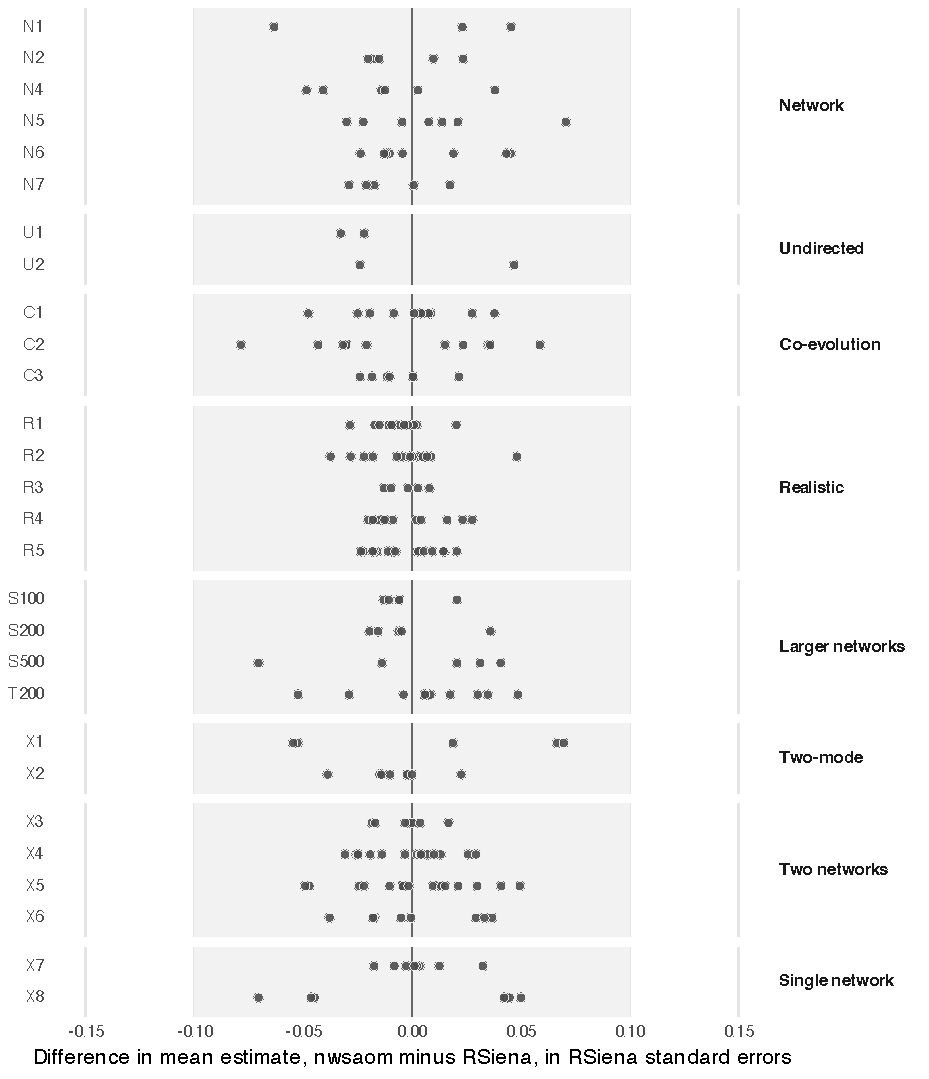
\includegraphics[width=\textwidth]{fig_bench_agree.pdf}
\caption{Difference between the mean estimates of \nwsaom{} and RSiena for every
parameter of every model, in RSiena standard errors; the band marks $\pm0.1$.}
\end{figure}

\section{Further models}\label{sec:benchextra}

The same comparison, with the same conventions (default settings of both programs, a fit counts as converged when RSiena's overall convergence ratio is below 0.25), for the later model families: eight models, X1 and X2 for two-mode networks, X3 to X6 for several networks (with and without a behavior, and with a non-directed network) and X7 and X8 for newer single-network effects. The data are the Glasgow friendship panel, a second randomly generated network and the smoking behavior (several networks), and simulated bipartite data (two-mode).

All eight models agree with RSiena: the largest difference of a mean estimate, rates included, is 0.07 RSiena standard errors.

Some effect sets were chosen so that RSiena converges: on the 40$\times$20 data \texttt{outactivity} together with \texttt{indegpopularity} and \texttt{cycle4} does not converge in RSiena, \texttt{antiiniso2} on the same data and the effects \texttt{Jin} and \texttt{Jout} together on the Glasgow data make \texttt{siena07} stop with ``thetaBound should be set higher'', and the \texttt{Jout} estimate in X8 is large (about 9.6, standard error about 4) in both programs. Some fits did not converge in one of the programs (RSiena: X1 two of eight seeds, X4 and X5 two each, X8 one; \nwsaom{}: X8 one); they are left out of the comparison and replaced by the next seed.

\section{Limits of this comparison}

\begin{itemize}
\item One data set (Glasgow and disconnected copies of it) for the one-mode models, and one specification per family for the later models; agreement may differ for other effects and for sparser or denser networks.
\item Both programs at default settings.
\item RSiena \benchrsiena{} (R \benchrver) was the reference version.
\end{itemize}

\appendix
\chapter{Effects reference}\label{app:effects}
All implemented effects, grouped as in RSiena's effects table. ``Network / context'' says which kind of dependent variable and which kind of interaction the row is for. The option column is what you type; \texttt{var}, \texttt{stem} and \texttt{matrix} stand for a variable, the stem of a changing covariate and a Stata matrix.
\subsection*{A. One-mode, non-directed and two-mode network: density and reciprocity}
\footnotesize
\begin{longtable}{@{}p{3.3cm}p{3.0cm}p{2.6cm}p{5.0cm}@{}}
\toprule
RSiena name & Network / context & Validated & nwsaom option\\
\midrule
\endhead
\opt{density} & one-mode network & siena07 & \opt{outdegree}\\
\opt{recip} & one-mode network & siena07 & \opt{reciprocity}\\
\opt{density} & two-mode network & siena07 & \opt{outdegree}\\
\opt{density} & non-directed network & siena07 & \opt{outdegree}\\
\bottomrule
\end{longtable}
\normalsize

\subsection*{B. Network structural effects: triadic and distance-two effects}
\footnotesize
\begin{longtable}{@{}p{3.3cm}p{3.0cm}p{2.6cm}p{5.0cm}@{}}
\toprule
RSiena name & Network / context & Validated & nwsaom option\\
\midrule
\endhead
\opt{transTrip} & one-mode network & siena07 & \opt{transtrip}\\
\opt{transTrip1} & one-mode network & siena07 & \opt{ownx(transtrip1)}\\
\opt{transTrip2} & one-mode network & siena07 & \opt{ownx(transtrip2)}\\
\opt{transMedTrip} & one-mode network & siena07 & \opt{transmedtrip}\\
\opt{transRecTrip} & one-mode network & siena07 & \opt{transrectrip}\\
\opt{transRecTrip2} & one-mode network & siena07 & \opt{ownx(transrectrip2)}\\
\opt{cycle3} & one-mode network & siena07 & \opt{cycle3}\\
\opt{transTies} & one-mode network & siena07 & \opt{transties}\\
\opt{between} & one-mode network & siena07 & \opt{between}\\
\opt{balance} & one-mode network & siena07 & \opt{balance}\\
\opt{nbrDist2} & one-mode network & siena07 & \opt{nbrdist2}\\
\opt{nbrDist2twice} & one-mode network & siena07 & \opt{dblnbrdist2}\\
\opt{denseTriads} & one-mode network & siena07 & \opt{ownx(densetriads:5)}\\
\opt{gwespFF} & one-mode network & siena07 & \opt{gwesp(\#)}\\
\opt{gwespBB} & one-mode network & siena07 & \opt{gwespbb(\#)}\\
\opt{gwespFB} & one-mode network & siena07 & \opt{gwespfb(\#)}\\
\opt{gwespBF} & one-mode network & siena07 & \opt{gwespbf(\#)}\\
\opt{gwespRR} & one-mode network & siena07 & \opt{gwesprr(\#)}\\
\opt{gwdspFF} & one-mode network & siena07 & \opt{gwdspff(\#)}\\
\opt{gwdspFB} & one-mode network & siena07 & \opt{gwdspfb(\#)}\\
\opt{sharedPop} & one-mode network & siena07 & \opt{cycle4 / sqrtcycle4}\\
\opt{cycle4} & one-mode network & siena07 & \opt{cycle4 / sqrtcycle4}\\
\opt{inStructEq} & one-mode network & siena07 & \opt{ownx(instructeq)}\\
\opt{Jin} & one-mode network & siena07 & \opt{ownx(jin)}\\
\opt{Jout} & one-mode network & siena07 & \opt{ownx(jout)}\\
\opt{transTrip.FR} & one-mode network & siena07 & \opt{ownx(transtripfr)}\\
\opt{transTrip.FE} & one-mode network & siena07 & \opt{ownx(transtripfe)}\\
\opt{transTrip.EE} & one-mode network & siena07 & \opt{ownx(transtripee)}\\
\opt{cycle4} & two-mode network & siena07 & \opt{cycle4}\\
\opt{gwdspFB} & two-mode network & siena07 & \opt{gwdspfb(0.69)}\\
\opt{transTriads} & non-directed network & siena07 & \opt{transtriads}\\
\opt{transTies} & non-directed network & siena07 & \opt{transties}\\
\opt{between} & non-directed network & siena07 & \opt{between}\\
\opt{balance} & non-directed network & siena07 & \opt{balance}\\
\opt{nbrDist2} & non-directed network & siena07 & \opt{nbrdist2}\\
\opt{nbrDist2twice} & non-directed network & siena07 & \opt{dblnbrdist2}\\
\opt{gwesp} & non-directed network & siena07 & \opt{gwesp(\#)}\\
\opt{cycle4} & non-directed network & siena07 & \opt{cycle4}\\
\opt{Jout} & non-directed network & siena07 & \opt{ownx(jout)}\\
\bottomrule
\end{longtable}
\normalsize

\subsection*{C. Network structural effects: degree effects (popularity, activity, assortativity, reciprocal degree)}
\footnotesize
\begin{longtable}{@{}p{3.3cm}p{3.0cm}p{2.6cm}p{5.0cm}@{}}
\toprule
RSiena name & Network / context & Validated & nwsaom option\\
\midrule
\endhead
\opt{inPop} & one-mode network & siena07 & \opt{inpop}\\
\opt{inPop.c} & one-mode network & siena07 & \opt{inpopc}\\
\opt{inPopSqrt} & one-mode network & siena07 & \opt{indegpopularity}\\
\opt{inPop\_dya} & one-mode network & siena07 & \opt{ownx(inpopdya)}\\
\opt{outPop} & one-mode network & siena07 & \opt{outpop}\\
\opt{outPop.c} & one-mode network & siena07 & \opt{outpopc}\\
\opt{outPopSqrt} & one-mode network & siena07 & \opt{outpopularity}\\
\opt{outPopMore} & one-mode network & siena07 & \opt{ownx(outpopmore:\#)}\\
\opt{outPopSqrtMore} & one-mode network & siena07 & \opt{ownx(outpopsqrtmore:\#)}\\
\opt{outPopThreshold} & one-mode network & siena07 & \opt{ownx(outpopthreshold:\#)}\\
\opt{reciPop} & one-mode network & siena07 & \opt{recipop}\\
\opt{reciPopSqrt} & one-mode network & siena07 & \opt{recipopsqrt}\\
\opt{inActSqrt} & one-mode network & siena07 & \opt{inactivity}\\
\opt{outAct} & one-mode network & siena07 & \opt{outactivity}\\
\opt{outAct.c} & one-mode network & siena07 & \opt{outactc}\\
\opt{outActSqrt} & one-mode network & siena07 & \opt{outactsqrt}\\
\opt{inAct} & one-mode network & siena07 & \opt{inact}\\
\opt{inAct.c} & one-mode network & siena07 & \opt{inactc}\\
\opt{reciAct} & one-mode network & siena07 & \opt{reciact / reciactsqrt}\\
\opt{avDeg} & one-mode network & siena07 & \opt{avdeg(c)}\\
\opt{outOutAss} & one-mode network & siena07 & \opt{ownx(outoutass)}\\
\opt{outInAss} & one-mode network & siena07 & \opt{ownx(outinass)}\\
\opt{inOutAss} & one-mode network & siena07 & \opt{ownx(inoutass)}\\
\opt{inInAss} & one-mode network & siena07 & \opt{ownx(ininass)}\\
\opt{outAct\_ego} & one-mode network & siena07 & \opt{ownx(outactego)}\\
\opt{outActMore\_ego} & one-mode network & siena07 & \opt{ownx(outactmoreego:\#)}\\
\opt{outActSqrtMore\_ego} & one-mode network & siena07 & \opt{ownx(outactsqrtmoreego:\#)}\\
\opt{outMore\_ego} & one-mode network & siena07 & \opt{ownx(outmoreego:\#)}\\
\opt{divOut\_ego} & one-mode network & siena07 & \opt{ownx(divoutego)}\\
\opt{inAct\_ego} & one-mode network & siena07 & \opt{ownx(inactego)}\\
\opt{divIn\_ego} & one-mode network & siena07 & \opt{ownx(divinego)}\\
\opt{reciAct\_ego} & one-mode network & siena07 & \opt{ownx(reciactego)}\\
\opt{inPop} & two-mode network & siena07 & \opt{inpop}\\
\opt{inPop.c} & two-mode network & siena07 & \opt{inpopc}\\
\opt{inPopSqrt} & two-mode network & siena07 & \opt{indegpopularity}\\
\opt{outAct} & two-mode network & siena07 & \opt{outactivity}\\
\opt{outAct.c} & two-mode network & siena07 & \opt{outactc}\\
\opt{outActSqrt} & two-mode network & siena07 & \opt{outactsqrt}\\
\opt{avDeg} & two-mode network & siena07 & \opt{avdeg(2)}\\
\opt{outInAss} & two-mode network & siena07 & \opt{ownx(outinass:2)}\\
\opt{outAct\_ego} & two-mode network & siena07 & \opt{ownx(outactego)}\\
\opt{divOut\_ego} & two-mode network & siena07 & \opt{ownx(divoutego:1)}\\
\opt{outActMore\_ego} & two-mode network & siena07 & \opt{ownx(outactmoreego:0)}\\
\opt{outActSqrtMore\_ego} & two-mode network & siena07 & \opt{ownx(outactsqrtmoreego:0)}\\
\opt{outMore\_ego} & two-mode network & siena07 & \opt{ownx(outmoreego:0)}\\
\opt{inPop} & non-directed network & siena07 & \opt{inpop}\\
\opt{inPop.c} & non-directed network & siena07 & \opt{inpopc}\\
\opt{inPopSqrt} & non-directed network & siena07 & \opt{indegpopularity}\\
\opt{inPop\_dya} & non-directed network & siena07 & \opt{ownx(inpopdya)}\\
\opt{outAct} & non-directed network & siena07 & \opt{outactivity}\\
\opt{outAct.c} & non-directed network & siena07 & \opt{outactc}\\
\opt{outActSqrt} & non-directed network & siena07 & \opt{outactsqrt}\\
\opt{degPlus} & non-directed network & siena07 & \opt{degplus}\\
\opt{degPlus.c} & non-directed network & siena07 & \opt{degplusc}\\
\opt{outInAss} & non-directed network & siena07 & \opt{ownx(outinass:2)}\\
\opt{divOut\_ego} & non-directed network & siena07 & \opt{ownx(divoutego:1)}\\
\opt{avDeg} & non-directed network & siena07 & \opt{avdeg(c)}\\
\bottomrule
\end{longtable}
\normalsize

\subsection*{D. Network structural effects: functions of the outdegree}
\footnotesize
\begin{longtable}{@{}p{3.3cm}p{3.0cm}p{2.6cm}p{5.0cm}@{}}
\toprule
RSiena name & Network / context & Validated & nwsaom option\\
\midrule
\endhead
\opt{outTrunc} & one-mode network & siena07 & \opt{outtrunc(\#)}\\
\opt{outTrunc2} & one-mode network & siena07 & \opt{outtrunc(\#), parameter value of RSiena outTrunc2}\\
\opt{outMore} & one-mode network & siena07 & \opt{outmore(\#)}\\
\opt{outMore2} & one-mode network & siena07 & \opt{outmore(\#), parameter value of RSiena outMore2}\\
\opt{outMore3} & one-mode network & siena07 & \opt{outmore(\#), parameter value of RSiena outMore3}\\
\opt{outThreshold} & one-mode network & siena07 & \opt{outthreshold(\#)}\\
\opt{outThreshold2} & one-mode network & siena07 & \opt{outthreshold(\#), parameter value of RSiena outThreshold2}\\
\opt{outInv} & one-mode network & siena07 & \opt{outinv(\#)}\\
\opt{outSqInv} & one-mode network & siena07 & \opt{outsqinv(\#)}\\
\opt{outTrunc} & two-mode network & siena07 & \opt{outtrunc(c)}\\
\opt{outTrunc2} & two-mode network & siena07 & \opt{outtrunc(5)}\\
\opt{outMore} & two-mode network & siena07 & \opt{outmore(c)}\\
\opt{outMore2} & two-mode network & siena07 & \opt{outmore(1)}\\
\opt{outMore3} & two-mode network & siena07 & \opt{outmore(1)}\\
\opt{outThreshold} & two-mode network & siena07 & \opt{outthreshold(c)}\\
\opt{outThreshold2} & two-mode network & siena07 & \opt{outthreshold(1)}\\
\opt{outInv} & two-mode network & siena07 & \opt{outinv(c)}\\
\opt{outSqInv} & two-mode network & siena07 & \opt{outsqinv(c)}\\
\opt{outTrunc} & non-directed network & siena07 & \opt{outtrunc(c)}\\
\opt{outTrunc2} & non-directed network & siena07 & \opt{outtrunc(5)}\\
\opt{outMore} & non-directed network & siena07 & \opt{outmore(c)}\\
\opt{outMore2} & non-directed network & siena07 & \opt{outmore(1)}\\
\opt{outMore3} & non-directed network & siena07 & \opt{outmore(1)}\\
\opt{outThreshold} & non-directed network & siena07 & \opt{outthreshold(c)}\\
\opt{outThreshold2} & non-directed network & siena07 & \opt{outthreshold(1)}\\
\opt{outInv} & non-directed network & siena07 & \opt{outinv(c)}\\
\opt{outSqInv} & non-directed network & siena07 & \opt{outsqinv(c)}\\
\bottomrule
\end{longtable}
\normalsize

\subsection*{E. Network structural effects: isolates and degree thresholds}
\footnotesize
\begin{longtable}{@{}p{3.3cm}p{3.0cm}p{2.6cm}p{5.0cm}@{}}
\toprule
RSiena name & Network / context & Validated & nwsaom option\\
\midrule
\endhead
\opt{outIso} & one-mode network & siena07 & \opt{outiso}\\
\opt{inIsDegree} & one-mode network & siena07 & \opt{ownx(inisdegree)}\\
\opt{isolateNet} & one-mode network & siena07 & \opt{isolatenet}\\
\opt{antiIso} & one-mode network & siena07 & \opt{antiiso}\\
\opt{antiInIso} & one-mode network & siena07 & \opt{antiiniso}\\
\opt{antiInIso2} & one-mode network & siena07 & \opt{antiiniso2}\\
\opt{in2Plus} & one-mode network & siena07 & \opt{antiiniso2}\\
\opt{in3Plus} & one-mode network & siena07 & \opt{inplus3}\\
\opt{isolatePop} & one-mode network & siena07 & \opt{isolatepop}\\
\opt{outIso} & two-mode network & siena07 & \opt{outiso}\\
\opt{antiInIso} & two-mode network & siena07 & \opt{antiiniso}\\
\opt{antiInIso2} & two-mode network & siena07 & \opt{antiiniso2}\\
\opt{in2Plus} & two-mode network & siena07 & \opt{antiiniso2}\\
\opt{in3Plus} & two-mode network & siena07 & \opt{inplus3}\\
\opt{outIso} & non-directed network & siena07 & \opt{outiso}\\
\opt{isolateNet} & non-directed network & siena07 & \opt{isolatenet}\\
\opt{antiInIso} & non-directed network & siena07 & \opt{antiiniso}\\
\opt{antiInIso2} & non-directed network & siena07 & \opt{antiiniso2}\\
\bottomrule
\end{longtable}
\normalsize

\subsection*{F. Network structural effects: compression, primary-setting and other}
\footnotesize
\begin{longtable}{@{}p{3.3cm}p{3.0cm}p{2.6cm}p{5.0cm}@{}}
\toprule
RSiena name & Network / context & Validated & nwsaom option\\
\midrule
\endhead
\opt{nonPCompress} & one-mode network & siena07 & \opt{ownx(nonpcompress)}\\
\opt{primCompress} & one-mode network & siena07 & \opt{ownx(primcompress)}\\
\opt{primary} & one-mode network & siena07 & \opt{ownx(primary)}\\
\opt{primDegAct} & one-mode network & siena07 & \opt{ownx(primdegact)}\\
\opt{primDegActLog} & one-mode network & siena07 & \opt{ownx(primdegactlog)}\\
\opt{primDegActSqrt} & one-mode network & siena07 & \opt{ownx(primdegactsqrt)}\\
\opt{primDegActInv} & one-mode network & siena07 & \opt{ownx(primdegactinv)}\\
\opt{primDegActDiff} & one-mode network & siena07 & \opt{ownx(primdegactdiff)}\\
\opt{primDegActDiffSqrt} & one-mode network & siena07 & \opt{ownx(primdegactdiffsqrt)}\\
\opt{unspInt} & one-mode network & siena07 & \opt{interact()}\\
\opt{unspInt} & two-mode network & siena07 & \opt{interact}\\
\opt{unspInt} & non-directed network & siena07 & \opt{symmetric + interact}\\
\bottomrule
\end{longtable}
\normalsize

\subsection*{G. Network effects of monadic covariates (constant covariate, coCovar)}
\footnotesize
\begin{longtable}{@{}p{3.3cm}p{3.0cm}p{2.6cm}p{5.0cm}@{}}
\toprule
RSiena name & Network / context & Validated & nwsaom option\\
\midrule
\endhead
\opt{altX} & one-mode network + constant covariate & siena07 & \opt{altx() / nodeicov()}\\
\opt{altSqX} & one-mode network + constant covariate & siena07 & \opt{altsqx()}\\
\opt{altLThresholdX} & one-mode network + constant covariate & siena07 & \opt{altlthresholdx()}\\
\opt{altRThresholdX} & one-mode network + constant covariate & siena07 & \opt{altrthresholdx()}\\
\opt{outXMore} & one-mode network + constant covariate & siena07 & \opt{netx(outxmore:var)}\\
\opt{egoX} & one-mode network + constant covariate & siena07 & \opt{egox() / nodeocov()}\\
\opt{egoSqX} & one-mode network + constant covariate & siena07 & \opt{egosqx()}\\
\opt{egoLThresholdX} & one-mode network + constant covariate & siena07 & \opt{egolthresholdx()}\\
\opt{egoRThresholdX} & one-mode network + constant covariate & siena07 & \opt{egorthresholdx()}\\
\opt{degAbsDiffX} & one-mode network + constant covariate & siena07 & \opt{degabsdiffx()}\\
\opt{degPosDiffX} & one-mode network + constant covariate & siena07 & \opt{degposdiffx()}\\
\opt{degNegDiffX} & one-mode network + constant covariate & siena07 & \opt{degnegdiffx()}\\
\opt{diffX} & one-mode network + constant covariate & siena07 & \opt{diffx()}\\
\opt{absDiffX} & one-mode network + constant covariate & siena07 & \opt{absdiffx()}\\
\opt{diffSqX} & one-mode network + constant covariate & siena07 & \opt{diffsqx()}\\
\opt{egoDiffX} & one-mode network + constant covariate & siena07 & \opt{egodiffx()}\\
\opt{egoPlusAltX} & one-mode network + constant covariate & siena07 & \opt{nodecov()}\\
\opt{altHigherEgoX} & one-mode network + constant covariate & siena07 & \opt{althigheregox()}\\
\opt{higher} & one-mode network + constant covariate & siena07 & \opt{higher()}\\
\opt{egoPlusAltSqX} & one-mode network + constant covariate & siena07 & \opt{egoplusaltsqx()}\\
\opt{simX} & one-mode network + constant covariate & siena07 & \opt{simx() / simcov()}\\
\opt{simRecipX} & one-mode network + constant covariate & siena07 & \opt{simrecipx()}\\
\opt{simXTransTrip} & one-mode network + constant covariate & siena07 & \opt{simxtranstrip()}\\
\opt{sameX} & one-mode network + constant covariate & siena07 & \opt{samex() / nodematch()}\\
\opt{unequalX} & one-mode network + constant covariate & siena07 & \opt{unequalx()}\\
\opt{sameXRecip} & one-mode network + constant covariate & siena07 & \opt{samexrecip()}\\
\opt{inPopX} & one-mode network + constant covariate & siena07 & \opt{inpopx()}\\
\opt{outPopX} & one-mode network + constant covariate & siena07 & \opt{outpopx()}\\
\opt{inActX} & one-mode network + constant covariate & siena07 & \opt{inactx()}\\
\opt{outActX} & one-mode network + constant covariate & siena07 & \opt{outactx()}\\
\opt{sameXInPop} & one-mode network + constant covariate & siena07 & \opt{samexinpop()}\\
\opt{diffXInPop} & one-mode network + constant covariate & siena07 & \opt{diffxinpop()}\\
\opt{sameXOutAct} & one-mode network + constant covariate & siena07 & \opt{samexoutact()}\\
\opt{diffXOutAct} & one-mode network + constant covariate & siena07 & \opt{diffxoutact()}\\
\opt{crossXOutAct} & one-mode network + constant covariate & siena07 & \opt{netx(crossxoutact:var)}\\
\opt{homXOutAct} & one-mode network + constant covariate & siena07 & \opt{homxoutact()}\\
\opt{homXOutAct2} & one-mode network + constant covariate & siena07 & \opt{netx(homxoutact2:var)}\\
\opt{altXOutAct} & one-mode network + constant covariate & siena07 & \opt{altxoutact()}\\
\opt{sameXReciAct} & one-mode network + constant covariate & siena07 & \opt{samexreciact()}\\
\opt{diffXReciAct} & one-mode network + constant covariate & siena07 & \opt{diffxreciact()}\\
\opt{transTripX} & one-mode network + constant covariate & siena07 & \opt{netx(transtripx:var)}\\
\opt{sameXTransTrip} & one-mode network + constant covariate & siena07 & \opt{samextranstrip()}\\
\opt{diffXTransTrip} & one-mode network + constant covariate & siena07 & \opt{diffxtranstrip()}\\
\opt{homXTransTrip} & one-mode network + constant covariate & siena07 & \opt{homxtranstrip()}\\
\opt{jumpXTransTrip} & one-mode network + constant covariate & siena07 & \opt{netx(jumpxtranstrip:var)}\\
\opt{homXTransRecTrip} & one-mode network + constant covariate & siena07 & \opt{netx(homxtransrectrip:var)}\\
\opt{sameXTransRecTrip} & one-mode network + constant covariate & siena07 & \opt{netx(samextransrectrip:var)}\\
\opt{diffXTransRecTrip} & one-mode network + constant covariate & siena07 & \opt{netx(diffxtransrectrip:var)}\\
\opt{sameXCycle4} & one-mode network + constant covariate & siena07 & \opt{netx(samexcycle4:var)}\\
\opt{sameInXCycle4} & one-mode network + constant covariate & siena07 & \opt{netx(sameinxcycle4:var)}\\
\opt{egoXaltX} & one-mode network + constant covariate & siena07 & \opt{egoxaltx()}\\
\opt{egoXaltXRecip} & one-mode network + constant covariate & siena07 & \opt{netx(egoxaltxrecip:var)}\\
\opt{IndTies} & one-mode network + constant covariate & siena07 & \opt{netx(indties:var)}\\
\opt{altDist2} & one-mode network + constant covariate & siena07 & \opt{netx(altdist2:var)}\\
\opt{totDist2} & one-mode network + constant covariate & siena07 & \opt{netx(totdist2:var)}\\
\opt{simDist2} & one-mode network + constant covariate & siena07 & \opt{netx(simdist2:var)}\\
\opt{simEgoDist2} & one-mode network + constant covariate & siena07 & \opt{netx(simegodist2:var)}\\
\opt{sameEgoDist2} & one-mode network + constant covariate & siena07 & \opt{netx(sameegodist2:var)}\\
\opt{altInDist2} & one-mode network + constant covariate & siena07 & \opt{netx(altindist2:var)}\\
\opt{totInDist2} & one-mode network + constant covariate & siena07 & \opt{netx(totindist2:var)}\\
\opt{simEgoInDist2} & one-mode network + constant covariate & siena07 & \opt{netx(simegoindist2:var)}\\
\opt{sameEgoInDist2} & one-mode network + constant covariate & siena07 & \opt{netx(sameegoindist2:var)}\\
\opt{egoX} & two-mode network + constant covariate & siena07 & \opt{nodeocov() / egox()}\\
\opt{egoSqX} & two-mode network + constant covariate & siena07 & \opt{egosqx(var)}\\
\opt{egoLThresholdX} & two-mode network + constant covariate & siena07 & \opt{egolthresholdx(varlist)}\\
\opt{egoRThresholdX} & two-mode network + constant covariate & siena07 & \opt{egorthresholdx(varlist)}\\
\opt{degAbsDiffX} & two-mode network + constant covariate & siena07 & \opt{degabsdiffx(varlist)}\\
\opt{degPosDiffX} & two-mode network + constant covariate & siena07 & \opt{degposdiffx(varlist)}\\
\opt{degNegDiffX} & two-mode network + constant covariate & siena07 & \opt{degnegdiffx(varlist)}\\
\opt{altInDist2} & two-mode network + constant covariate & siena07 & \opt{netx(altindist2:var)}\\
\opt{totInDist2} & two-mode network + constant covariate & siena07 & \opt{netx(totindist2:var)}\\
\opt{simEgoInDist2} & two-mode network + constant covariate & siena07 & \opt{netx(simegoindist2:var)}\\
\opt{sameEgoInDist2} & two-mode network + constant covariate & siena07 & \opt{netx(sameegoindist2:var)}\\
\opt{inPopX} & two-mode network + constant covariate & siena07 & \opt{inpopx(varlist)}\\
\opt{sameXInPop} & two-mode network + constant covariate & siena07 & \opt{samexinpop(varlist)}\\
\opt{diffXInPop} & two-mode network + constant covariate & siena07 & \opt{diffxinpop(varlist)}\\
\opt{crossXOutAct} & two-mode network + constant covariate & siena07 & \opt{netx(crossxoutact:var)}\\
\opt{sameXCycle4} & two-mode network + constant covariate & siena07 & \opt{netx(samexcycle4:var)}\\
\opt{altX} & two-mode network + constant covariate & siena07 & \opt{nodeicov() / altx()}\\
\opt{altSqX} & two-mode network + constant covariate & siena07 & \opt{altsqx(var)}\\
\opt{altLThresholdX} & two-mode network + constant covariate & siena07 & \opt{altlthresholdx(varlist)}\\
\opt{altRThresholdX} & two-mode network + constant covariate & siena07 & \opt{altrthresholdx(varlist)}\\
\opt{outActX} & two-mode network + constant covariate & siena07 & \opt{outactx(varlist)}\\
\opt{sameInXCycle4} & two-mode network + constant covariate & siena07 & \opt{netx(sameinxcycle4:var)}\\
\opt{homXOutAct} & two-mode network + constant covariate & siena07 & \opt{homxoutact(varlist)}\\
\opt{homXOutAct2} & two-mode network + constant covariate & siena07 & \opt{netx(homxoutact2:var) xparam(3)}\\
\opt{altXOutAct} & two-mode network + constant covariate & siena07 & \opt{altxoutact(varlist)}\\
\opt{altX} & non-directed network + constant covariate & siena07 & \opt{altx()}\\
\opt{altSqX} & non-directed network + constant covariate & siena07 & \opt{altsqx()}\\
\opt{altLThresholdX} & non-directed network + constant covariate & siena07 & \opt{altlthresholdx()}\\
\opt{altRThresholdX} & non-directed network + constant covariate & siena07 & \opt{altrthresholdx()}\\
\opt{outXMore} & non-directed network + constant covariate & siena07 & \opt{netx(outxmore:var)}\\
\opt{egoX} & non-directed network + constant covariate & siena07 & \opt{egox()}\\
\opt{egoSqX} & non-directed network + constant covariate & siena07 & \opt{egosqx()}\\
\opt{egoPlusAltX} & non-directed network + constant covariate & siena07 & \opt{nodecov()}\\
\opt{egoPlusAltSqX} & non-directed network + constant covariate & siena07 & \opt{egoplusaltsqx()}\\
\opt{egoLThresholdX} & non-directed network + constant covariate & siena07 & \opt{egolthresholdx()}\\
\opt{egoRThresholdX} & non-directed network + constant covariate & siena07 & \opt{egorthresholdx()}\\
\opt{degAbsDiffX} & non-directed network + constant covariate & siena07 & \opt{degabsdiffx()}\\
\opt{degPosDiffX} & non-directed network + constant covariate & siena07 & \opt{degposdiffx()}\\
\opt{degNegDiffX} & non-directed network + constant covariate & siena07 & \opt{degnegdiffx()}\\
\opt{diffX} & non-directed network + constant covariate & siena07 & \opt{diffx()}\\
\opt{absDiffX} & non-directed network + constant covariate & siena07 & \opt{absdiffx()}\\
\opt{diffSqX} & non-directed network + constant covariate & siena07 & \opt{diffsqx()}\\
\opt{egoDiffX} & non-directed network + constant covariate & siena07 & \opt{egodiffx()}\\
\opt{altHigherEgoX} & non-directed network + constant covariate & siena07 & \opt{althigheregox()}\\
\opt{higher} & non-directed network + constant covariate & siena07 & \opt{higher()}\\
\opt{simX} & non-directed network + constant covariate & siena07 & \opt{simx()}\\
\opt{inPopX} & non-directed network + constant covariate & siena07 & \opt{inpopx()}\\
\opt{outPopX} & non-directed network + constant covariate & siena07 & \opt{outpopx()}\\
\opt{inActX} & non-directed network + constant covariate & siena07 & \opt{inactx()}\\
\opt{outActX} & non-directed network + constant covariate & siena07 & \opt{outactx()}\\
\opt{sameX} & non-directed network + constant covariate & siena07 & \opt{samex()}\\
\opt{unequalX} & non-directed network + constant covariate & siena07 & \opt{unequalx()}\\
\opt{sameXInPop} & non-directed network + constant covariate & siena07 & \opt{samexinpop()}\\
\opt{diffXInPop} & non-directed network + constant covariate & siena07 & \opt{diffxinpop()}\\
\opt{sameXOutAct} & non-directed network + constant covariate & siena07 & \opt{samexoutact()}\\
\opt{diffXOutAct} & non-directed network + constant covariate & siena07 & \opt{diffxoutact()}\\
\opt{crossXOutAct} & non-directed network + constant covariate & siena07 & \opt{netx(crossxoutact:var)}\\
\opt{homXOutAct} & non-directed network + constant covariate & siena07 & \opt{homxoutact()}\\
\opt{homXOutAct2} & non-directed network + constant covariate & siena07 & \opt{netx(homxoutact2:var)}\\
\opt{altXOutAct} & non-directed network + constant covariate & siena07 & \opt{altxoutact()}\\
\opt{transTripX} & non-directed network + constant covariate & siena07 & \opt{netx(transtripx:var)}\\
\opt{sameXTransTrip} & non-directed network + constant covariate & siena07 & \opt{samextranstrip()}\\
\opt{diffXTransTrip} & non-directed network + constant covariate & siena07 & \opt{diffxtranstrip()}\\
\opt{homXTransTrip} & non-directed network + constant covariate & siena07 & \opt{homxtranstrip()}\\
\opt{jumpXTransTrip} & non-directed network + constant covariate & siena07 & \opt{netx(jumpxtranstrip:var)}\\
\opt{sameXCycle4} & non-directed network + constant covariate & siena07 & \opt{netx(samexcycle4:var)}\\
\opt{sameInXCycle4} & non-directed network + constant covariate & siena07 & \opt{netx(sameinxcycle4:var)}\\
\opt{egoXaltX} & non-directed network + constant covariate & siena07 & \opt{egoxaltx()}\\
\opt{IndTies} & non-directed network + constant covariate & siena07 & \opt{netx(indties:var)}\\
\opt{altDist2} & non-directed network + constant covariate & siena07 & \opt{netx(altdist2:var)}\\
\opt{totDist2} & non-directed network + constant covariate & siena07 & \opt{netx(totdist2:var)}\\
\opt{simEgoDist2} & non-directed network + constant covariate & siena07 & \opt{netx(simegodist2:var)}\\
\opt{sameEgoDist2} & non-directed network + constant covariate & siena07 & \opt{netx(sameegodist2:var)}\\
\opt{simDist2} & non-directed network + constant covariate & siena07 & \opt{netx(simdist2:var)}\\
\opt{altInDist2} & non-directed network + constant covariate & siena07 & \opt{netx(altindist2:var)}\\
\opt{totInDist2} & non-directed network + constant covariate & siena07 & \opt{netx(totindist2:var)}\\
\opt{simEgoInDist2} & non-directed network + constant covariate & siena07 & \opt{netx(simegoindist2:var)}\\
\bottomrule
\end{longtable}
\normalsize

\subsection*{H. Network effects of monadic covariates (changing covariate, varCovar)}
\footnotesize
\begin{longtable}{@{}p{3.3cm}p{3.0cm}p{2.6cm}p{5.0cm}@{}}
\toprule
RSiena name & Network / context & Validated & nwsaom option\\
\midrule
\endhead
\opt{altX} & one-mode network + changing covariate & siena07 & \opt{altx() with a tvcov stem}\\
\opt{altSqX} & one-mode network + changing covariate & siena07 & \opt{altsqx() with a tvcov stem}\\
\opt{altLThresholdX} & one-mode network + changing covariate & siena07 & \opt{altlthresholdx() with a tvcov stem}\\
\opt{altRThresholdX} & one-mode network + changing covariate & siena07 & \opt{altrthresholdx() with a tvcov stem}\\
\opt{outXMore} & one-mode network + changing covariate & siena07 & \opt{netx(outxmore:var)}\\
\opt{egoX} & one-mode network + changing covariate & siena07 & \opt{egox() with a tvcov stem}\\
\opt{egoSqX} & one-mode network + changing covariate & siena07 & \opt{egosqx() with a tvcov stem}\\
\opt{egoLThresholdX} & one-mode network + changing covariate & siena07 & \opt{egolthresholdx() with a tvcov stem}\\
\opt{egoRThresholdX} & one-mode network + changing covariate & siena07 & \opt{egorthresholdx() with a tvcov stem}\\
\opt{degAbsDiffX} & one-mode network + changing covariate & siena07 & \opt{degabsdiffx() with a tvcov stem}\\
\opt{degPosDiffX} & one-mode network + changing covariate & siena07 & \opt{degposdiffx() with a tvcov stem}\\
\opt{degNegDiffX} & one-mode network + changing covariate & siena07 & \opt{degnegdiffx() with a tvcov stem}\\
\opt{diffX} & one-mode network + changing covariate & siena07 & \opt{diffx() with a tvcov stem}\\
\opt{absDiffX} & one-mode network + changing covariate & siena07 & \opt{absdiffx() with a tvcov stem}\\
\opt{diffSqX} & one-mode network + changing covariate & siena07 & \opt{diffsqx() with a tvcov stem}\\
\opt{egoDiffX} & one-mode network + changing covariate & siena07 & \opt{egodiffx() with a tvcov stem}\\
\opt{egoPlusAltX} & one-mode network + changing covariate & siena07 & \opt{nodecov() with a tvcov stem}\\
\opt{altHigherEgoX} & one-mode network + changing covariate & siena07 & \opt{althigheregox() with a tvcov stem}\\
\opt{higher} & one-mode network + changing covariate & siena07 & \opt{higher() with a tvcov stem}\\
\opt{egoPlusAltSqX} & one-mode network + changing covariate & siena07 & \opt{egoplusaltsqx() with a tvcov stem}\\
\opt{simX} & one-mode network + changing covariate & siena07 & \opt{simx() with a tvcov stem}\\
\opt{simRecipX} & one-mode network + changing covariate & siena07 & \opt{netx(simrecipx:var) / netbeh(simrecipx)}\\
\opt{simXTransTrip} & one-mode network + changing covariate & siena07 & \opt{netx(simxtranstrip:var) / netbeh(simxtranstrip)}\\
\opt{sameX} & one-mode network + changing covariate & siena07 & \opt{samex() with a tvcov stem}\\
\opt{unequalX} & one-mode network + changing covariate & siena07 & \opt{unequalx() with a tvcov stem}\\
\opt{sameXRecip} & one-mode network + changing covariate & siena07 & \opt{samexrecip() with a tvcov stem}\\
\opt{inPopX} & one-mode network + changing covariate & siena07 & \opt{inpopx() with a tvcov stem}\\
\opt{outPopX} & one-mode network + changing covariate & siena07 & \opt{outpopx() with a tvcov stem}\\
\opt{inActX} & one-mode network + changing covariate & siena07 & \opt{inactx() with a tvcov stem}\\
\opt{outActX} & one-mode network + changing covariate & siena07 & \opt{outactx() with a tvcov stem}\\
\opt{sameXInPop} & one-mode network + changing covariate & siena07 & \opt{samexinpop() with a tvcov stem}\\
\opt{diffXInPop} & one-mode network + changing covariate & siena07 & \opt{diffxinpop() with a tvcov stem}\\
\opt{sameXOutAct} & one-mode network + changing covariate & siena07 & \opt{samexoutact() with a tvcov stem}\\
\opt{diffXOutAct} & one-mode network + changing covariate & siena07 & \opt{diffxoutact() with a tvcov stem}\\
\opt{crossXOutAct} & one-mode network + changing covariate & siena07 & \opt{netx(crossxoutact:var)}\\
\opt{homXOutAct} & one-mode network + changing covariate & siena07 & \opt{homxoutact() with a tvcov stem}\\
\opt{homXOutAct2} & one-mode network + changing covariate & siena07 & \opt{netx(homxoutact2:var)}\\
\opt{altXOutAct} & one-mode network + changing covariate & siena07 & \opt{altxoutact() with a tvcov stem}\\
\opt{sameXReciAct} & one-mode network + changing covariate & siena07 & \opt{samexreciact() with a tvcov stem}\\
\opt{diffXReciAct} & one-mode network + changing covariate & siena07 & \opt{diffxreciact() with a tvcov stem}\\
\opt{transTripX} & one-mode network + changing covariate & siena07 & \opt{netx(transtripx:var)}\\
\opt{sameXTransTrip} & one-mode network + changing covariate & siena07 & \opt{samextranstrip() with a tvcov stem}\\
\opt{diffXTransTrip} & one-mode network + changing covariate & siena07 & \opt{diffxtranstrip() with a tvcov stem}\\
\opt{homXTransTrip} & one-mode network + changing covariate & siena07 & \opt{homxtranstrip() with a tvcov stem}\\
\opt{jumpXTransTrip} & one-mode network + changing covariate & siena07 & \opt{netx(jumpxtranstrip:var)}\\
\opt{homXTransRecTrip} & one-mode network + changing covariate & siena07 & \opt{netx(homxtransrectrip:var)}\\
\opt{sameXTransRecTrip} & one-mode network + changing covariate & siena07 & \opt{netx(samextransrectrip:var)}\\
\opt{diffXTransRecTrip} & one-mode network + changing covariate & siena07 & \opt{netx(diffxtransrectrip:var)}\\
\opt{sameXCycle4} & one-mode network + changing covariate & siena07 & \opt{netx(samexcycle4:var)}\\
\opt{sameInXCycle4} & one-mode network + changing covariate & siena07 & \opt{netx(sameinxcycle4:var)}\\
\opt{egoXaltX} & one-mode network + changing covariate & siena07 & \opt{egoxaltx() with a tvcov stem}\\
\opt{egoXaltXRecip} & one-mode network + changing covariate & siena07 & \opt{netx(egoxaltxrecip:var)}\\
\opt{IndTies} & one-mode network + changing covariate & siena07 & \opt{netx(indties:var)}\\
\opt{altDist2} & one-mode network + changing covariate & siena07 & \opt{netx(altdist2:var)}\\
\opt{totDist2} & one-mode network + changing covariate & siena07 & \opt{netx(totdist2:var)}\\
\opt{simDist2} & one-mode network + changing covariate & siena07 & \opt{netx(simdist2:var)}\\
\opt{simEgoDist2} & one-mode network + changing covariate & siena07 & \opt{netx(simegodist2:var)}\\
\opt{sameEgoDist2} & one-mode network + changing covariate & siena07 & \opt{netx(sameegodist2:var)}\\
\opt{altInDist2} & one-mode network + changing covariate & siena07 & \opt{netx(altindist2:var)}\\
\opt{totInDist2} & one-mode network + changing covariate & siena07 & \opt{netx(totindist2:var)}\\
\opt{simEgoInDist2} & one-mode network + changing covariate & siena07 & \opt{netx(simegoindist2:var)}\\
\opt{sameEgoInDist2} & one-mode network + changing covariate & siena07 & \opt{netx(sameegoindist2:var)}\\
\opt{avGroupEgoX} & one-mode network + changing covariate & siena07 & \opt{netx(avgroupegox:var)}\\
\opt{totGroupEgoX} & one-mode network + changing covariate & siena07 & \opt{netx(totgroupegox:var)}\\
\opt{egoX} & two-mode network + changing covariate & siena07 & \opt{nodeocov(tvstem)}\\
\opt{egoSqX} & two-mode network + changing covariate & siena07 & \opt{egosqx(tvstem)}\\
\opt{egoLThresholdX} & two-mode network + changing covariate & siena07 & \opt{egolthresholdx(varlist)}\\
\opt{egoRThresholdX} & two-mode network + changing covariate & siena07 & \opt{egorthresholdx(varlist)}\\
\opt{degAbsDiffX} & two-mode network + changing covariate & siena07 & \opt{degabsdiffx(varlist)}\\
\opt{degPosDiffX} & two-mode network + changing covariate & siena07 & \opt{degposdiffx(varlist)}\\
\opt{degNegDiffX} & two-mode network + changing covariate & siena07 & \opt{degnegdiffx(varlist)}\\
\opt{altInDist2} & two-mode network + changing covariate & siena07 & \opt{netx(altindist2:tvstem)}\\
\opt{totInDist2} & two-mode network + changing covariate & siena07 & \opt{netx(totindist2:tvstem)}\\
\opt{simEgoInDist2} & two-mode network + changing covariate & siena07 & \opt{netx(simegoindist2:tvstem)}\\
\opt{sameEgoInDist2} & two-mode network + changing covariate & siena07 & \opt{netx(sameegoindist2:tvstem)}\\
\opt{inPopX} & two-mode network + changing covariate & siena07 & \opt{inpopx(varlist)}\\
\opt{sameXInPop} & two-mode network + changing covariate & siena07 & \opt{samexinpop(varlist)}\\
\opt{diffXInPop} & two-mode network + changing covariate & siena07 & \opt{diffxinpop(varlist)}\\
\opt{crossXOutAct} & two-mode network + changing covariate & siena07 & \opt{netx(crossxoutact:tvstem)}\\
\opt{sameXCycle4} & two-mode network + changing covariate & siena07 & \opt{netx(samexcycle4:tvstem)}\\
\opt{avGroupEgoX} & two-mode network + changing covariate & siena07 & \opt{netx(avgroupegox:tvstem)}\\
\opt{totGroupEgoX} & two-mode network + changing covariate & siena07 & \opt{netx(totgroupegox:tvstem)}\\
\opt{altX} & non-directed network + changing covariate & siena07 & \opt{altx()}\\
\opt{altSqX} & non-directed network + changing covariate & siena07 & \opt{altsqx()}\\
\opt{altLThresholdX} & non-directed network + changing covariate & siena07 & \opt{altlthresholdx()}\\
\opt{altRThresholdX} & non-directed network + changing covariate & siena07 & \opt{altrthresholdx()}\\
\opt{outXMore} & non-directed network + changing covariate & siena07 & \opt{netx(outxmore:var)}\\
\opt{egoX} & non-directed network + changing covariate & siena07 & \opt{egox()}\\
\opt{egoSqX} & non-directed network + changing covariate & siena07 & \opt{egosqx()}\\
\opt{egoPlusAltX} & non-directed network + changing covariate & siena07 & \opt{tvcov() + nodecov(stem)}\\
\opt{egoPlusAltSqX} & non-directed network + changing covariate & siena07 & \opt{egoplusaltsqx()}\\
\opt{egoLThresholdX} & non-directed network + changing covariate & siena07 & \opt{egolthresholdx()}\\
\opt{egoRThresholdX} & non-directed network + changing covariate & siena07 & \opt{egorthresholdx()}\\
\opt{degAbsDiffX} & non-directed network + changing covariate & siena07 & \opt{degabsdiffx()}\\
\opt{degPosDiffX} & non-directed network + changing covariate & siena07 & \opt{degposdiffx()}\\
\opt{degNegDiffX} & non-directed network + changing covariate & siena07 & \opt{degnegdiffx()}\\
\opt{diffX} & non-directed network + changing covariate & siena07 & \opt{diffx()}\\
\opt{absDiffX} & non-directed network + changing covariate & siena07 & \opt{absdiffx()}\\
\opt{diffSqX} & non-directed network + changing covariate & siena07 & \opt{diffsqx()}\\
\opt{egoDiffX} & non-directed network + changing covariate & siena07 & \opt{egodiffx()}\\
\opt{altHigherEgoX} & non-directed network + changing covariate & siena07 & \opt{althigheregox()}\\
\opt{higher} & non-directed network + changing covariate & siena07 & \opt{symmetric higher}\\
\opt{simX} & non-directed network + changing covariate & siena07 & \opt{simx()}\\
\opt{inPopX} & non-directed network + changing covariate & siena07 & \opt{inpopx()}\\
\opt{outPopX} & non-directed network + changing covariate & siena07 & \opt{outpopx()}\\
\opt{inActX} & non-directed network + changing covariate & siena07 & \opt{inactx()}\\
\opt{outActX} & non-directed network + changing covariate & siena07 & \opt{outactx()}\\
\opt{sameX} & non-directed network + changing covariate & siena07 & \opt{samex()}\\
\opt{unequalX} & non-directed network + changing covariate & siena07 & \opt{unequalx()}\\
\opt{sameXInPop} & non-directed network + changing covariate & siena07 & \opt{samexinpop()}\\
\opt{diffXInPop} & non-directed network + changing covariate & siena07 & \opt{diffxinpop()}\\
\opt{sameXOutAct} & non-directed network + changing covariate & siena07 & \opt{samexoutact()}\\
\opt{diffXOutAct} & non-directed network + changing covariate & siena07 & \opt{diffxoutact()}\\
\opt{crossXOutAct} & non-directed network + changing covariate & siena07 & \opt{netx(crossxoutact:var)}\\
\opt{homXOutAct} & non-directed network + changing covariate & siena07 & \opt{homxoutact()}\\
\opt{homXOutAct2} & non-directed network + changing covariate & siena07 & \opt{netx(homxoutact2:var)}\\
\opt{altXOutAct} & non-directed network + changing covariate & siena07 & \opt{altxoutact()}\\
\opt{transTripX} & non-directed network + changing covariate & siena07 & \opt{netx(transtripx:var)}\\
\opt{sameXTransTrip} & non-directed network + changing covariate & siena07 & \opt{samextranstrip()}\\
\opt{diffXTransTrip} & non-directed network + changing covariate & siena07 & \opt{diffxtranstrip()}\\
\opt{homXTransTrip} & non-directed network + changing covariate & siena07 & \opt{homxtranstrip()}\\
\opt{jumpXTransTrip} & non-directed network + changing covariate & siena07 & \opt{netx(jumpxtranstrip:var)}\\
\opt{sameXCycle4} & non-directed network + changing covariate & siena07 & \opt{netx(samexcycle4:var)}\\
\opt{sameInXCycle4} & non-directed network + changing covariate & siena07 & \opt{netx(sameinxcycle4:var)}\\
\opt{egoXaltX} & non-directed network + changing covariate & siena07 & \opt{egoxaltx()}\\
\opt{IndTies} & non-directed network + changing covariate & siena07 & \opt{netx(indties:var)}\\
\opt{altDist2} & non-directed network + changing covariate & siena07 & \opt{netx(altdist2:var)}\\
\opt{totDist2} & non-directed network + changing covariate & siena07 & \opt{netx(totdist2:var)}\\
\opt{simEgoDist2} & non-directed network + changing covariate & siena07 & \opt{netx(simegodist2:var)}\\
\opt{sameEgoDist2} & non-directed network + changing covariate & siena07 & \opt{netx(sameegodist2:var)}\\
\opt{simDist2} & non-directed network + changing covariate & siena07 & \opt{netx(simdist2:var)}\\
\opt{altInDist2} & non-directed network + changing covariate & siena07 & \opt{netx(altindist2:var)}\\
\opt{totInDist2} & non-directed network + changing covariate & siena07 & \opt{netx(totindist2:var)}\\
\opt{simEgoInDist2} & non-directed network + changing covariate & siena07 & \opt{netx(simegoindist2:var)}\\
\opt{avGroupEgoX} & non-directed network + changing covariate & siena07 & \opt{netx(avgroupegox:var)}\\
\opt{totGroupEgoX} & non-directed network + changing covariate & siena07 & \opt{netx(totgroupegox:var)}\\
\bottomrule
\end{longtable}
\normalsize

\subsection*{I. Network effects of two covariates (double covariate effects)}
\footnotesize
\begin{longtable}{@{}p{3.3cm}p{3.0cm}p{2.6cm}p{5.0cm}@{}}
\toprule
RSiena name & Network / context & Validated & nwsaom option\\
\midrule
\endhead
\opt{sameXV} & one-mode network + constant covariate + constant covariate & siena07 & \opt{netx(samexv:var1:var2)}\\
\opt{sameXVInPop} & one-mode network + constant covariate + constant covariate & siena07 & \opt{netx(samexvinpop:var1:var2)}\\
\opt{sameXVInPop2} & one-mode network + constant covariate + constant covariate & siena07 & \opt{netx(samexvinpop2:var1:var2)}\\
\bottomrule
\end{longtable}
\normalsize

\subsection*{J. Network effects of dyadic covariates (coDyadCovar, varDyadCovar)}
\footnotesize
\begin{longtable}{@{}p{3.3cm}p{3.0cm}p{2.6cm}p{5.0cm}@{}}
\toprule
RSiena name & Network / context & Validated & nwsaom option\\
\midrule
\endhead
\opt{X} & one-mode network + constant dyadic covariate & siena07 & \opt{dyadcov()}\\
\opt{XRecip} & one-mode network + constant dyadic covariate & siena07 & \opt{dyadcovrecip()}\\
\opt{WWX} & one-mode network + constant dyadic covariate & siena07 & \opt{dyadx(wwx:matrix)}\\
\opt{cyWWX} & one-mode network + constant dyadic covariate & siena07 & \opt{dyadx(cywwx:matrix)}\\
\opt{InWWX} & one-mode network + constant dyadic covariate & siena07 & \opt{dyadx(inwwx:matrix)}\\
\opt{OutWWX} & one-mode network + constant dyadic covariate & siena07 & \opt{dyadx(outwwx:matrix)}\\
\opt{WXX} & one-mode network + constant dyadic covariate & siena07 & \opt{dyadx(wxx:matrix)}\\
\opt{XWX} & one-mode network + constant dyadic covariate & siena07 & \opt{dyadx(xwx:matrix)}\\
\opt{XWX1} & one-mode network + constant dyadic covariate & siena07 & \opt{dyadx(xwx1:matrix)}\\
\opt{XWX2} & one-mode network + constant dyadic covariate & siena07 & \opt{dyadx(xwx2:matrix)}\\
\opt{XXW} & one-mode network + constant dyadic covariate & siena07 & \opt{dyadx(xxw:matrix)}\\
\opt{X} & one-mode network + changing dyadic covariate & siena07 & \opt{tvdyadcov(stem)}\\
\opt{XRecip} & one-mode network + changing dyadic covariate & siena07 & \opt{tvdyadcovrecip(stem)}\\
\opt{WWX} & one-mode network + changing dyadic covariate & siena07 & \opt{tvdyadx(wwx:stem)}\\
\opt{cyWWX} & one-mode network + changing dyadic covariate & siena07 & \opt{tvdyadx(cywwx:stem)}\\
\opt{InWWX} & one-mode network + changing dyadic covariate & siena07 & \opt{tvdyadx(inwwx:stem)}\\
\opt{OutWWX} & one-mode network + changing dyadic covariate & siena07 & \opt{tvdyadx(outwwx:stem)}\\
\opt{WXX} & one-mode network + changing dyadic covariate & siena07 & \opt{tvdyadx(wxx:stem)}\\
\opt{XWX} & one-mode network + changing dyadic covariate & siena07 & \opt{tvdyadx(xwx:stem)}\\
\opt{XWX1} & one-mode network + changing dyadic covariate & siena07 & \opt{tvdyadx(xwx1:stem)}\\
\opt{XWX2} & one-mode network + changing dyadic covariate & siena07 & \opt{tvdyadx(xwx2:stem)}\\
\opt{XXW} & one-mode network + changing dyadic covariate & siena07 & \opt{tvdyadx(xxw:stem)}\\
\opt{X} & two-mode network + constant dyadic covariate & siena07 & \opt{dyadcov}\\
\opt{X} & non-directed network + constant dyadic covariate & siena07 & \opt{dyadcov()}\\
\opt{XRecip} & non-directed network + constant dyadic covariate & siena07 & \opt{dyadcovrecip()}\\
\opt{WWX} & non-directed network + constant dyadic covariate & siena07 & \opt{dyadx(wwx:matrix)}\\
\opt{cyWWX} & non-directed network + constant dyadic covariate & siena07 & \opt{dyadx(cywwx:matrix)}\\
\opt{InWWX} & non-directed network + constant dyadic covariate & siena07 & \opt{dyadx(inwwx:matrix)}\\
\opt{OutWWX} & non-directed network + constant dyadic covariate & siena07 & \opt{dyadx(outwwx:matrix)}\\
\opt{WXX} & non-directed network + constant dyadic covariate & siena07 & \opt{dyadx(wxx:matrix)}\\
\opt{XWX} & non-directed network + constant dyadic covariate & siena07 & \opt{dyadx(xwx:matrix)}\\
\opt{XWX1} & non-directed network + constant dyadic covariate & siena07 & \opt{dyadx(xwx1:matrix)}\\
\opt{XWX2} & non-directed network + constant dyadic covariate & siena07 & \opt{dyadx(xwx2:matrix)}\\
\opt{XXW} & non-directed network + constant dyadic covariate & siena07 & \opt{dyadx(xxw:matrix)}\\
\opt{X} & non-directed network + changing dyadic covariate & siena07 & \opt{tvdyadcov(stem)}\\
\opt{XRecip} & non-directed network + changing dyadic covariate & siena07 & \opt{symmetric tvdyadcovrecip}\\
\opt{WWX} & non-directed network + changing dyadic covariate & siena07 & \opt{tvdyadx(wwx:stem)}\\
\opt{cyWWX} & non-directed network + changing dyadic covariate & siena07 & \opt{tvdyadx(cywwx:stem)}\\
\opt{InWWX} & non-directed network + changing dyadic covariate & siena07 & \opt{tvdyadx(inwwx:stem)}\\
\opt{OutWWX} & non-directed network + changing dyadic covariate & siena07 & \opt{tvdyadx(outwwx:stem)}\\
\opt{WXX} & non-directed network + changing dyadic covariate & siena07 & \opt{tvdyadx(wxx:stem)}\\
\opt{XWX} & non-directed network + changing dyadic covariate & siena07 & \opt{tvdyadx(xwx:stem)}\\
\opt{XWX1} & non-directed network + changing dyadic covariate & siena07 & \opt{tvdyadx(xwx1:stem)}\\
\opt{XWX2} & non-directed network + changing dyadic covariate & siena07 & \opt{tvdyadx(xwx2:stem)}\\
\opt{XXW} & non-directed network + changing dyadic covariate & siena07 & \opt{tvdyadx(xxw:stem)}\\
\bottomrule
\end{longtable}
\normalsize

\subsection*{K. Network effects of a dependent behavior variable (behavior as covariate: selection)}
\footnotesize
\begin{longtable}{@{}p{3.3cm}p{3.0cm}p{2.6cm}p{5.0cm}@{}}
\toprule
RSiena name & Network / context & Validated & nwsaom option\\
\midrule
\endhead
\opt{altX} & one-mode network + a behavior variable & siena07 & \opt{behaltx}\\
\opt{altSqX} & one-mode network + a behavior variable & siena07 & \opt{netbeh(altsqx)}\\
\opt{altLThresholdX} & one-mode network + a behavior variable & siena07 & \opt{netbeh(altlthresholdx)}\\
\opt{altRThresholdX} & one-mode network + a behavior variable & siena07 & \opt{netbeh(altrthresholdx)}\\
\opt{outXMore} & one-mode network + a behavior variable & siena07 & \opt{netbeh(outxmore)}\\
\opt{egoX} & one-mode network + a behavior variable & siena07 & \opt{behegox}\\
\opt{egoSqX} & one-mode network + a behavior variable & siena07 & \opt{netbeh(egosqx)}\\
\opt{egoLThresholdX} & one-mode network + a behavior variable & siena07 & \opt{netbeh(egolthresholdx)}\\
\opt{egoRThresholdX} & one-mode network + a behavior variable & siena07 & \opt{netbeh(egorthresholdx)}\\
\opt{degAbsDiffX} & one-mode network + a behavior variable & siena07 & \opt{netbeh(degabsdiffx)}\\
\opt{degPosDiffX} & one-mode network + a behavior variable & siena07 & \opt{netbeh(degposdiffx)}\\
\opt{degNegDiffX} & one-mode network + a behavior variable & siena07 & \opt{netbeh(degnegdiffx)}\\
\opt{diffX} & one-mode network + a behavior variable & siena07 & \opt{netbeh(diffx)}\\
\opt{absDiffX} & one-mode network + a behavior variable & siena07 & \opt{netbeh(absdiffx)}\\
\opt{diffSqX} & one-mode network + a behavior variable & siena07 & \opt{netbeh(diffsqx)}\\
\opt{egoDiffX} & one-mode network + a behavior variable & siena07 & \opt{netbeh(egodiffx)}\\
\opt{egoPlusAltX} & one-mode network + a behavior variable & siena07 & \opt{behegoplusalt}\\
\opt{altHigherEgoX} & one-mode network + a behavior variable & siena07 & \opt{netbeh(althigheregox)}\\
\opt{higher} & one-mode network + a behavior variable & siena07 & \opt{netbeh(higher)}\\
\opt{egoPlusAltSqX} & one-mode network + a behavior variable & siena07 & \opt{netbeh(egoplusaltsqx)}\\
\opt{simX} & one-mode network + a behavior variable & siena07 & \opt{behsim}\\
\opt{simRecipX} & one-mode network + a behavior variable & siena07 & \opt{netx(simrecipx:var) / netbeh(simrecipx)}\\
\opt{simXTransTrip} & one-mode network + a behavior variable & siena07 & \opt{netx(simxtranstrip:var) / netbeh(simxtranstrip)}\\
\opt{sameX} & one-mode network + a behavior variable & siena07 & \opt{netbeh(samex)}\\
\opt{unequalX} & one-mode network + a behavior variable & siena07 & \opt{netbeh(unequalx)}\\
\opt{sameXRecip} & one-mode network + a behavior variable & siena07 & \opt{netbeh(samexrecip)}\\
\opt{inPopX} & one-mode network + a behavior variable & siena07 & \opt{netbeh(inpopx)}\\
\opt{outPopX} & one-mode network + a behavior variable & siena07 & \opt{netbeh(outpopx)}\\
\opt{inActX} & one-mode network + a behavior variable & siena07 & \opt{netbeh(inactx)}\\
\opt{outActX} & one-mode network + a behavior variable & siena07 & \opt{netbeh(outactx)}\\
\opt{sameXInPop} & one-mode network + a behavior variable & siena07 & \opt{netbeh(samexinpop)}\\
\opt{diffXInPop} & one-mode network + a behavior variable & siena07 & \opt{netbeh(diffxinpop)}\\
\opt{sameXOutAct} & one-mode network + a behavior variable & siena07 & \opt{netbeh(samexoutact)}\\
\opt{diffXOutAct} & one-mode network + a behavior variable & siena07 & \opt{netbeh(diffxoutact)}\\
\opt{crossXOutAct} & one-mode network + a behavior variable & siena07 & \opt{netbeh(crossxoutact)}\\
\opt{homXOutAct} & one-mode network + a behavior variable & siena07 & \opt{netbeh(homxoutact)}\\
\opt{altXOutAct} & one-mode network + a behavior variable & siena07 & \opt{netbeh(altxoutact)}\\
\opt{sameXReciAct} & one-mode network + a behavior variable & siena07 & \opt{netbeh(samexreciact)}\\
\opt{diffXReciAct} & one-mode network + a behavior variable & siena07 & \opt{netbeh(diffxreciact)}\\
\opt{transTripX} & one-mode network + a behavior variable & siena07 & \opt{netbeh(transtripx)}\\
\opt{sameXTransTrip} & one-mode network + a behavior variable & siena07 & \opt{netbeh(samextranstrip)}\\
\opt{diffXTransTrip} & one-mode network + a behavior variable & siena07 & \opt{netbeh(diffxtranstrip)}\\
\opt{homXTransTrip} & one-mode network + a behavior variable & siena07 & \opt{netbeh(homxtranstrip)}\\
\opt{jumpXTransTrip} & one-mode network + a behavior variable & siena07 & \opt{netbeh(jumpxtranstrip)}\\
\opt{homXTransRecTrip} & one-mode network + a behavior variable & siena07 & \opt{netbeh(homxtransrectrip)}\\
\opt{sameXTransRecTrip} & one-mode network + a behavior variable & siena07 & \opt{netbeh(samextransrectrip)}\\
\opt{diffXTransRecTrip} & one-mode network + a behavior variable & siena07 & \opt{netbeh(diffxtransrectrip)}\\
\opt{sameXCycle4} & one-mode network + a behavior variable & siena07 & \opt{netbeh(samexcycle4)}\\
\opt{sameInXCycle4} & one-mode network + a behavior variable & siena07 & \opt{netbeh(sameinxcycle4)}\\
\opt{egoXaltX} & one-mode network + a behavior variable & siena07 & \opt{netbeh(egoxaltx)}\\
\opt{egoXaltXRecip} & one-mode network + a behavior variable & siena07 & \opt{netbeh(egoxaltxrecip)}\\
\opt{IndTies} & one-mode network + a behavior variable & siena07 & \opt{netbeh(indties)}\\
\opt{altDist2} & one-mode network + a behavior variable & siena07 & \opt{netbeh(altdist2)}\\
\opt{totDist2} & one-mode network + a behavior variable & siena07 & \opt{netbeh(totdist2)}\\
\opt{simDist2} & one-mode network + a behavior variable & siena07 & \opt{netbeh(simdist2)}\\
\opt{simEgoDist2} & one-mode network + a behavior variable & siena07 & \opt{netbeh(simegodist2)}\\
\opt{sameEgoDist2} & one-mode network + a behavior variable & siena07 & \opt{netbeh(sameegodist2)}\\
\opt{altInDist2} & one-mode network + a behavior variable & siena07 & \opt{netbeh(altindist2)}\\
\opt{totInDist2} & one-mode network + a behavior variable & siena07 & \opt{netbeh(totindist2)}\\
\opt{simEgoInDist2} & one-mode network + a behavior variable & siena07 & \opt{netbeh(simegoindist2)}\\
\opt{sameEgoInDist2} & one-mode network + a behavior variable & siena07 & \opt{netbeh(sameegoindist2)}\\
\opt{avGroupEgoX} & one-mode network + a behavior variable & siena07 & \opt{netbeh(avgroupegox)}\\
\opt{totGroupEgoX} & one-mode network + a behavior variable & siena07 & \opt{netbeh(totgroupegox)}\\
\opt{egoX} & two-mode network + a behavior variable & siena07 & \opt{behavior() + behegox}\\
\opt{egoSqX} & two-mode network + a behavior variable & siena07 & \opt{behavior() + netbeh(egosqx)}\\
\opt{egoLThresholdX} & two-mode network + a behavior variable & siena07 & \opt{egolthresholdx(varlist)}\\
\opt{egoRThresholdX} & two-mode network + a behavior variable & siena07 & \opt{egorthresholdx(varlist)}\\
\opt{degAbsDiffX} & two-mode network + a behavior variable & siena07 & \opt{degabsdiffx(varlist)}\\
\opt{degPosDiffX} & two-mode network + a behavior variable & siena07 & \opt{degposdiffx(varlist)}\\
\opt{degNegDiffX} & two-mode network + a behavior variable & siena07 & \opt{degnegdiffx(varlist)}\\
\opt{altInDist2} & two-mode network + a behavior variable & siena07 & \opt{behavior() + netbeh(altindist2)}\\
\opt{totInDist2} & two-mode network + a behavior variable & siena07 & \opt{behavior() + netbeh(totindist2)}\\
\opt{simEgoInDist2} & two-mode network + a behavior variable & siena07 & \opt{behavior() + netbeh(simegoindist2)}\\
\opt{sameEgoInDist2} & two-mode network + a behavior variable & siena07 & \opt{behavior() + netbeh(sameegoindist2)}\\
\opt{inPopX} & two-mode network + a behavior variable & siena07 & \opt{inpopx(varlist)}\\
\opt{sameXInPop} & two-mode network + a behavior variable & siena07 & \opt{samexinpop(varlist)}\\
\opt{diffXInPop} & two-mode network + a behavior variable & siena07 & \opt{diffxinpop(varlist)}\\
\opt{crossXOutAct} & two-mode network + a behavior variable & siena07 & \opt{behavior}\\
\opt{sameXCycle4} & two-mode network + a behavior variable & siena07 & \opt{behavior() + netbeh(samexcycle4)}\\
\opt{avGroupEgoX} & two-mode network + a behavior variable & siena07 & \opt{netbeh}\\
\opt{totGroupEgoX} & two-mode network + a behavior variable & siena07 & \opt{netbeh}\\
\opt{altX} & non-directed network + a behavior variable & siena07 & \opt{behaltx}\\
\opt{altSqX} & non-directed network + a behavior variable & siena07 & \opt{netbeh(altsqx)}\\
\opt{altLThresholdX} & non-directed network + a behavior variable & siena07 & \opt{netbeh(altlthresholdx)}\\
\opt{altRThresholdX} & non-directed network + a behavior variable & siena07 & \opt{netbeh(altrthresholdx)}\\
\opt{outXMore} & non-directed network + a behavior variable & siena07 & \opt{netbeh(outxmore)}\\
\opt{egoX} & non-directed network + a behavior variable & siena07 & \opt{behegox}\\
\opt{egoSqX} & non-directed network + a behavior variable & siena07 & \opt{netbeh(egosqx)}\\
\opt{egoPlusAltX} & non-directed network + a behavior variable & siena07 & \opt{behegoplusalt}\\
\opt{egoPlusAltSqX} & non-directed network + a behavior variable & siena07 & \opt{netbeh(egoplusaltsqx)}\\
\opt{egoLThresholdX} & non-directed network + a behavior variable & siena07 & \opt{netbeh(egolthresholdx)}\\
\opt{egoRThresholdX} & non-directed network + a behavior variable & siena07 & \opt{netbeh(egorthresholdx)}\\
\opt{degAbsDiffX} & non-directed network + a behavior variable & siena07 & \opt{symmetric + behavior}\\
\opt{degPosDiffX} & non-directed network + a behavior variable & siena07 & \opt{netbeh}\\
\opt{degNegDiffX} & non-directed network + a behavior variable & siena07 & \opt{netbeh(degnegdiffx)}\\
\opt{diffX} & non-directed network + a behavior variable & siena07 & \opt{netbeh(diffx)}\\
\opt{absDiffX} & non-directed network + a behavior variable & siena07 & \opt{netbeh(absdiffx)}\\
\opt{diffSqX} & non-directed network + a behavior variable & siena07 & \opt{netbeh(diffsqx)}\\
\opt{egoDiffX} & non-directed network + a behavior variable & siena07 & \opt{netbeh(egodiffx)}\\
\opt{altHigherEgoX} & non-directed network + a behavior variable & siena07 & \opt{netbeh(althigheregox)}\\
\opt{higher} & non-directed network + a behavior variable & siena07 & \opt{netbeh}\\
\opt{simX} & non-directed network + a behavior variable & siena07 & \opt{behsim}\\
\opt{inPopX} & non-directed network + a behavior variable & siena07 & \opt{netbeh(inpopx)}\\
\opt{outPopX} & non-directed network + a behavior variable & siena07 & \opt{netbeh(outpopx)}\\
\opt{inActX} & non-directed network + a behavior variable & siena07 & \opt{netbeh(inactx)}\\
\opt{outActX} & non-directed network + a behavior variable & siena07 & \opt{netbeh(outactx)}\\
\opt{sameX} & non-directed network + a behavior variable & siena07 & \opt{netbeh(samex)}\\
\opt{unequalX} & non-directed network + a behavior variable & siena07 & \opt{netbeh(unequalx)}\\
\opt{sameXInPop} & non-directed network + a behavior variable & siena07 & \opt{netbeh(samexinpop)}\\
\opt{diffXInPop} & non-directed network + a behavior variable & siena07 & \opt{netbeh(diffxinpop)}\\
\opt{sameXOutAct} & non-directed network + a behavior variable & siena07 & \opt{netbeh(samexoutact)}\\
\opt{diffXOutAct} & non-directed network + a behavior variable & siena07 & \opt{netbeh(diffxoutact)}\\
\opt{crossXOutAct} & non-directed network + a behavior variable & siena07 & \opt{netbeh(crossxoutact)}\\
\opt{homXOutAct} & non-directed network + a behavior variable & siena07 & \opt{netbeh(homxoutact)}\\
\opt{altXOutAct} & non-directed network + a behavior variable & siena07 & \opt{netbeh(altxoutact)}\\
\opt{transTripX} & non-directed network + a behavior variable & siena07 & \opt{netbeh(transtripx)}\\
\opt{sameXTransTrip} & non-directed network + a behavior variable & siena07 & \opt{netbeh(samextranstrip)}\\
\opt{diffXTransTrip} & non-directed network + a behavior variable & siena07 & \opt{netbeh(diffxtranstrip)}\\
\opt{homXTransTrip} & non-directed network + a behavior variable & siena07 & \opt{netbeh(homxtranstrip)}\\
\opt{jumpXTransTrip} & non-directed network + a behavior variable & siena07 & \opt{netbeh(jumpxtranstrip)}\\
\opt{sameXCycle4} & non-directed network + a behavior variable & siena07 & \opt{netbeh(samexcycle4)}\\
\opt{sameInXCycle4} & non-directed network + a behavior variable & siena07 & \opt{netbeh(sameinxcycle4)}\\
\opt{egoXaltX} & non-directed network + a behavior variable & siena07 & \opt{netbeh(egoxaltx)}\\
\opt{IndTies} & non-directed network + a behavior variable & siena07 & \opt{netbeh(indties)}\\
\opt{altDist2} & non-directed network + a behavior variable & siena07 & \opt{netbeh(altdist2)}\\
\opt{totDist2} & non-directed network + a behavior variable & siena07 & \opt{netbeh(totdist2)}\\
\opt{simEgoDist2} & non-directed network + a behavior variable & siena07 & \opt{netbeh(simegodist2)}\\
\opt{sameEgoDist2} & non-directed network + a behavior variable & siena07 & \opt{netbeh(sameegodist2)}\\
\opt{simDist2} & non-directed network + a behavior variable & siena07 & \opt{netbeh(simdist2)}\\
\opt{altInDist2} & non-directed network + a behavior variable & siena07 & \opt{netbeh(altindist2)}\\
\opt{totInDist2} & non-directed network + a behavior variable & siena07 & \opt{netbeh(totindist2)}\\
\opt{simEgoInDist2} & non-directed network + a behavior variable & siena07 & \opt{netbeh(simegoindist2)}\\
\opt{avGroupEgoX} & non-directed network + a behavior variable & siena07 & \opt{netbeh(avgroupegox)}\\
\opt{totGroupEgoX} & non-directed network + a behavior variable & siena07 & \opt{netbeh(totgroupegox)}\\
\bottomrule
\end{longtable}
\normalsize

\subsection*{L. Cross-network effects (several dependent networks)}
\footnotesize
\begin{longtable}{@{}p{3.3cm}p{3.0cm}p{2.6cm}p{5.0cm}@{}}
\toprule
RSiena name & Network / context & Validated & nwsaom option\\
\midrule
\endhead
\opt{from.w.ind} & one-mode network + another network + another network & siena07 & \opt{cross1}\\
\opt{crprod} & one-mode network + another network & siena07 & \opt{nwsaom multinet, cross1(crprod)}\\
\opt{crprodRecip} & one-mode network + another network & siena07 & \opt{nwsaom multinet, cross1(crprodrecip)}\\
\opt{crprodMutual} & one-mode network + another network & siena07 & \opt{nwsaom multinet, cross1(crprodmutual)}\\
\opt{inPopIntn} & one-mode network + another network & siena07 & \opt{nwsaom multinet, cross1(inpopintn)}\\
\opt{inActIntn} & one-mode network + another network & siena07 & \opt{nwsaom multinet, cross1(inactintn)}\\
\opt{crprodInActIntn} & one-mode network + another network & siena07 & \opt{nwsaom multinet, cross1(crprodinactintn)}\\
\opt{outPopIntn} & one-mode network + another network & siena07 & \opt{nwsaom multinet, cross1(outpopintn)}\\
\opt{outActIntn} & one-mode network + another network & siena07 & \opt{nwsaom multinet, cross1(outactintn)}\\
\opt{divOutEgoIntn} & one-mode network + another network & siena07 & \opt{nwsaom multinet, cross1(divoutegointn)}\\
\opt{divInEgoIntn} & one-mode network + another network & siena07 & \opt{nwsaom multinet, cross1(divinegointn)}\\
\opt{divOutAltIntn} & one-mode network + another network & siena07 & \opt{nwsaom multinet, cross1(divoutaltintn)}\\
\opt{divInAltIntn} & one-mode network + another network & siena07 & \opt{nwsaom multinet, cross1(divinaltintn)}\\
\opt{outOutActIntn} & one-mode network + another network & siena07 & \opt{nwsaom multinet, cross1(outoutactintn)}\\
\opt{outOutAvIntn} & one-mode network + another network & siena07 & \opt{nwsaom multinet, cross1(outoutavintn)}\\
\opt{dist2OutInActIntn} & one-mode network + another network & siena07 & \opt{nwsaom multinet, cross1(dist2outinactintn)}\\
\opt{outOutDist2ActIntn} & one-mode network + another network & siena07 & \opt{nwsaom multinet, cross1(outoutdist2actintn)}\\
\opt{avAlt.2M.tot} & one-mode network + another network & siena07 & \opt{nwsaom multinet, cross1(avalt2mtot)}\\
\opt{avDegIntn} & one-mode network + another network & siena07 & \opt{nwsaom multinet, cross1(avdegintn)}\\
\opt{absOutDiffIntn} & one-mode network + another network & siena07 & \opt{nwsaom multinet, cross1(absoutdiffintn)}\\
\opt{both} & one-mode network + another network & siena07 & \opt{nwsaom multinet, cross1(both)}\\
\opt{doubleOutAct} & one-mode network + another network & siena07 & \opt{nwsaom multinet, cross1(doubleoutact)}\\
\opt{doubleInPop} & one-mode network + another network & siena07 & \opt{nwsaom multinet, cross1(doubleinpop)}\\
\opt{betweenPop} & one-mode network + another network & siena07 & \opt{cross1}\\
\opt{from} & one-mode network + another network & siena07 & \opt{nwsaom multinet, cross1(from)}\\
\opt{fromMutual} & one-mode network + another network & siena07 & \opt{nwsaom multinet, cross1(frommutual)}\\
\opt{fromAny} & one-mode network + another network & siena07 & \opt{nwsaom multinet, cross1(fromany)}\\
\opt{to} & one-mode network + another network & siena07 & \opt{nwsaom multinet, cross1(to)}\\
\opt{toBack} & one-mode network + another network & siena07 & \opt{nwsaom multinet, cross1(toback)}\\
\opt{toRecip} & one-mode network + another network & siena07 & \opt{nwsaom multinet, cross1(torecip)}\\
\opt{toAny} & one-mode network + another network & siena07 & \opt{cross1}\\
\opt{cl.XWX} & one-mode network + another network & siena07 & \opt{nwsaom multinet, cross1(clxwx)}\\
\opt{cl.XWX1} & one-mode network + another network & siena07 & \opt{nwsaom multinet, cross1(clxwx1)}\\
\opt{cl.XWX2} & one-mode network + another network & siena07 & \opt{nwsaom multinet, cross1(clxwx2)}\\
\opt{WWX.EE} & one-mode network + another network & siena07 & \opt{nwsaom multinet, cross1(wwxee)}\\
\opt{WWX.FR} & one-mode network + another network & siena07 & \opt{nwsaom multinet, cross1(wwxfr)}\\
\opt{WXX.FE} & one-mode network + another network & siena07 & \opt{nwsaom multinet, cross1(wxxfe)}\\
\opt{WXX.ER} & one-mode network + another network & siena07 & \opt{nwsaom multinet, cross1(wxxer)}\\
\opt{XWX.ER} & one-mode network + another network & siena07 & \opt{nwsaom multinet, cross1(xwxer)}\\
\opt{XWX.FE} & one-mode network + another network & siena07 & \opt{nwsaom multinet, cross1(xwxfe)}\\
\opt{closure} & one-mode network + another network & siena07 & \opt{nwsaom multinet, cross1(closure)}\\
\opt{cyClosure} & one-mode network + another network & siena07 & \opt{nwsaom multinet, cross1(cyclosure)}\\
\opt{sharedIn} & one-mode network + another network & siena07 & \opt{nwsaom multinet, cross1(sharedin)}\\
\opt{mixedInXW} & one-mode network + another network & siena07 & \opt{nwsaom multinet, cross1(mixedinxw)}\\
\opt{sharedTo} & one-mode network + another network & siena07 & \opt{nwsaom multinet, cross1(sharedto)}\\
\opt{avAlt.2M.tie} & one-mode network + another network & siena07 & \opt{nwsaom multinet, cross1(avalt2mtie)}\\
\opt{inPopOutW} & one-mode network + another network & siena07 & \opt{nwsaom multinet, cross1(inpopoutw)}\\
\opt{nDist2ActIntn} & one-mode network + another network & siena07 & \opt{nwsaom multinet, cross1(ndist2actintn)}\\
\opt{JinMix} & one-mode network + another network & siena07 & \opt{nwsaom multinet, cross1(jinmix)}\\
\opt{JoutMix} & one-mode network + another network & siena07 & \opt{nwsaom multinet, cross1(joutmix)}\\
\opt{gwespFFMix} & one-mode network + another network & siena07 & \opt{nwsaom multinet, cross1(gwespffmix)}\\
\opt{gwespBBMix} & one-mode network + another network & siena07 & \opt{nwsaom multinet, cross1(gwespbbmix)}\\
\opt{gwespBFMix} & one-mode network + another network & siena07 & \opt{nwsaom multinet, cross1(gwespbfmix)}\\
\opt{gwespFBMix} & one-mode network + another network & siena07 & \opt{nwsaom multinet, cross1(gwespfbmix)}\\
\opt{gwespRRMix} & one-mode network + another network & siena07 & \opt{nwsaom multinet, cross1(gwesprrmix)}\\
\opt{gwespMix} & one-mode network + another network & siena07 & \opt{nwsaom multinet cross1(gwespfbmix)}\\
\opt{inActIntn} & two-mode network + another network & siena07 & \opt{cross1}\\
\opt{outActIntn} & two-mode network + another network & siena07 & \opt{cross1}\\
\opt{divOutEgoIntn} & two-mode network + another network & siena07 & \opt{cross1}\\
\opt{divInEgoIntn} & two-mode network + another network & siena07 & \opt{cross1}\\
\opt{divInAltIntn} & two-mode network + another network & siena07 & \opt{cross1}\\
\opt{avDegIntn} & two-mode network + another network & siena07 & \opt{cross1}\\
\opt{outOutActIntn} & two-mode network + another network & siena07 & \opt{cross1}\\
\opt{outOutAvIntn} & two-mode network + another network & siena07 & \opt{cross1}\\
\opt{dist2OutInActIntn} & two-mode network + another network & siena07 & \opt{cross1}\\
\opt{outOutDist2ActIntn} & two-mode network + another network & siena07 & \opt{cross1}\\
\opt{avAlt.2M.tot} & two-mode network + another network & siena07 & \opt{cross1}\\
\opt{to} & two-mode network + another network & siena07 & \opt{cross1}\\
\opt{toBack} & two-mode network + another network & siena07 & \opt{cross1}\\
\opt{toRecip} & two-mode network + another network & siena07 & \opt{cross1}\\
\opt{sharedTo} & two-mode network + another network & siena07 & \opt{cross1}\\
\opt{avAlt.2M.tie} & two-mode network + another network & siena07 & \opt{cross1}\\
\opt{inPopOutW} & two-mode network + another network & siena07 & \opt{cross1}\\
\opt{nDist2ActIntn} & two-mode network + another network & siena07 & \opt{cross1}\\
\opt{toAny} & two-mode network + another network & siena07 & \opt{cross1}\\
\opt{JoutMix} & two-mode network + another network & siena07 & \opt{cross1}\\
\opt{gwespFBMix} & two-mode network + another network & siena07 & \opt{cross1}\\
\opt{from.w.ind} & non-directed network + another network + another network & siena07 & \opt{cross1}\\
\opt{outPopIntn} & non-directed network + another network & siena07 & \opt{nwsaom multinet sym1 cross1(outpopintn)}\\
\opt{outActIntn} & non-directed network + another network & siena07 & \opt{nwsaom multinet sym1 cross1(outactintn)}\\
\opt{divOutEgoIntn} & non-directed network + another network & siena07 & \opt{nwsaom multinet sym1 cross1(divoutegointn)}\\
\opt{divInEgoIntn} & non-directed network + another network & siena07 & \opt{nwsaom multinet sym1 cross1(divinegointn)}\\
\opt{avDegIntn} & non-directed network + another network & siena07 & \opt{nwsaom multinet sym1 cross1(avdegintn)}\\
\opt{from} & non-directed network + another network & siena07 & \opt{nwsaom multinet sym1 cross1(from)}\\
\opt{fromAny} & non-directed network + another network & siena07 & \opt{nwsaom multinet sym1 cross1(fromany)}\\
\opt{to} & non-directed network + another network & siena07 & \opt{nwsaom multinet sym1 cross1(to)}\\
\opt{toAny} & non-directed network + another network & siena07 & \opt{cross1}\\
\opt{cl.XWX} & non-directed network + another network & siena07 & \opt{nwsaom multinet sym1 cross1(clxwx)}\\
\opt{closure} & non-directed network + another network & siena07 & \opt{nwsaom multinet sym1 cross1(closure)}\\
\opt{mixedInXW} & non-directed network + another network & siena07 & \opt{nwsaom multinet sym1 cross1(mixedinxw)}\\
\opt{JoutMix} & non-directed network + another network & siena07 & \opt{nwsaom multinet sym1 cross1(joutmix)}\\
\opt{gwespMix} & non-directed network + another network & siena07 & \opt{cross1}\\
\opt{crprod} & non-directed network + another network & siena07 & \opt{nwsaom multinet sym1 cross1(crprod)}\\
\opt{outOutActIntn} & non-directed network + another network & siena07 & \opt{cross1}\\
\opt{outOutAvIntn} & non-directed network + another network & siena07 & \opt{cross1}\\
\opt{dist2OutInActIntn} & non-directed network + another network & siena07 & \opt{nwsaom multinet sym1 cross1(dist2outinactintn)}\\
\opt{outOutDist2ActIntn} & non-directed network + another network & siena07 & \opt{nwsaom multinet sym1 cross1(outoutdist2actintn)}\\
\opt{outOutDist2AvIntn} & non-directed network + another network & siena07 & \opt{NOT IMPLEMENTED}\\
\opt{both} & non-directed network + another network & siena07 & \opt{cross1}\\
\opt{absOutDiffIntn} & non-directed network + another network & siena07 & \opt{nwsaom multinet sym1 cross1(absoutdiffintn)}\\
\opt{doubleOutAct} & non-directed network + another network & siena07 & \opt{nwsaom multinet sym1 cross1(doubleoutact)}\\
\opt{sharedTo} & non-directed network + another network & siena07 & \opt{nwsaom multinet sym1 cross1(sharedto)}\\
\opt{avAlt.2M.tie} & non-directed network + another network & siena07 & \opt{cross1}\\
\opt{inPopOutW} & non-directed network + another network & siena07 & \opt{nwsaom multinet sym1 cross1(inpopoutw)}\\
\opt{nDist2ActIntn} & non-directed network + another network & siena07 & \opt{nwsaom multinet sym1 cross1(ndist2actintn)}\\
\bottomrule
\end{longtable}
\normalsize

\subsection*{M. Cross-network effects combined with a covariate, a behavior or a dyadic covariate}
\footnotesize
\begin{longtable}{@{}p{3.3cm}p{3.0cm}p{2.6cm}p{5.0cm}@{}}
\toprule
RSiena name & Network / context & Validated & nwsaom option\\
\midrule
\endhead
\opt{sameWWClosure} & one-mode network + another network + constant covariate & siena07 & \opt{nwsaom multinet cross1(samewwclosure:var)}\\
\opt{diffWWClosure} & one-mode network + another network + constant covariate & siena07 & \opt{nwsaom multinet cross1(diffwwclosure:var)}\\
\opt{jumpWWClosure} & one-mode network + another network + constant covariate & siena07 & \opt{nwsaom multinet cross1(jumpwwclosure:var)}\\
\opt{jumpFrom} & one-mode network + another network + constant covariate & siena07 & \opt{nwsaom multinet cross1(jumpfrom:var)}\\
\opt{jumpSharedIn} & one-mode network + another network + constant covariate & siena07 & \opt{nwsaom multinet cross1(jumpsharedin:var)}\\
\opt{sameWXClosure} & one-mode network + another network + constant covariate & siena07 & \opt{nwsaom multinet cross1(samewxclosure:var)}\\
\opt{diffWXClosure} & one-mode network + another network + constant covariate & siena07 & \opt{nwsaom multinet cross1(diffwxclosure:var)}\\
\opt{jumpWXClosure} & one-mode network + another network + constant covariate & siena07 & \opt{nwsaom multinet cross1(jumpwxclosure:var)}\\
\opt{homWXClosure} & one-mode network + another network + constant covariate & siena07 & \opt{nwsaom multinet cross1(homwxclosure:var)}\\
\opt{sameXWClosure} & one-mode network + another network + constant covariate & siena07 & \opt{nwsaom multinet cross1(samexwclosure:var)}\\
\opt{diffXWClosure} & one-mode network + another network + constant covariate & siena07 & \opt{nwsaom multinet cross1(diffxwclosure:var)}\\
\opt{homCovNetNet} & one-mode network + another network + constant covariate & siena07 & \opt{nwsaom multinet cross1(homcovnetnet:var)}\\
\opt{contrastCovNetNet} & one-mode network + another network + constant covariate & siena07 & \opt{nwsaom multinet cross1(contrastcovnetnet:var)}\\
\opt{allDifCovNetNet} & one-mode network + another network + constant covariate & siena07 & \opt{nwsaom multinet cross1(alldifcovnetnet:var)}\\
\opt{homCovNetNetIn} & one-mode network + another network + constant covariate & siena07 & \opt{nwsaom multinet cross1(homcovnetnetin:var)}\\
\opt{contrastCovNetNetIn} & one-mode network + another network + constant covariate & siena07 & \opt{nwsaom multinet cross1(contrastcovnetnetin:var)}\\
\opt{allDifCovNetNetIn} & one-mode network + another network + constant covariate & siena07 & \opt{nwsaom multinet cross1(alldifcovnetnetin:var)}\\
\opt{simEgoDist2W} & one-mode network + another network + constant covariate & siena07 & \opt{nwsaom multinet cross1(simegodist2w:var)}\\
\opt{altInDist2W} & one-mode network + another network + constant covariate & siena07 & \opt{nwsaom multinet cross1(altindist2w:var)}\\
\opt{totInDist2W} & one-mode network + another network + constant covariate & siena07 & \opt{nwsaom multinet cross1(totindist2w:var)}\\
\opt{inActIntnX} & one-mode network + another network + constant covariate & siena07 & \opt{nwsaom multinet cross1(inactintnx:var)}\\
\opt{sameXInActIntn} & one-mode network + another network + constant covariate & siena07 & \opt{nwsaom multinet cross1(samexinactintn:var)}\\
\opt{covNetNet} & one-mode network + another network + constant covariate & siena07 & \opt{nwsaom multinet cross1(covnetnet:var)}\\
\opt{covNetNetIn} & one-mode network + another network + constant covariate & siena07 & \opt{nwsaom multinet cross1(covnetnetin:var)}\\
\opt{inPopIntnX} & one-mode network + another network + constant covariate & siena07 & \opt{nwsaom multinet cross1(inpopintnx:var)}\\
\opt{sameXInPopIntn} & one-mode network + another network + constant covariate & siena07 & \opt{nwsaom multinet cross1(samexinpopintn:var)}\\
\opt{simEgoInDist2W} & one-mode network + another network + constant covariate & siena07 & \opt{nwsaom multinet cross1(simegoindist2w:var)}\\
\opt{outPopIntnX} & one-mode network + another network + constant covariate & siena07 & \opt{nwsaom multinet cross1(outpopintnx:var)}\\
\opt{outActIntnX} & one-mode network + another network + constant covariate & siena07 & \opt{nwsaom multinet cross1(outactintnx:var)}\\
\opt{sameXOutPopIntn} & one-mode network + another network + constant covariate & siena07 & \opt{nwsaom multinet cross1(samexoutpopintn:var)}\\
\opt{sameXOutActIntn} & one-mode network + another network + constant covariate & siena07 & \opt{nwsaom multinet cross1(samexoutactintn:var)}\\
\opt{altDist2W} & one-mode network + another network + constant covariate & siena07 & \opt{nwsaom multinet cross1(altdist2w:var)}\\
\opt{totDist2W} & one-mode network + another network + constant covariate & siena07 & \opt{nwsaom multinet cross1(totdist2w:var)}\\
\opt{simDist2W} & one-mode network + another network + constant covariate & siena07 & \opt{nwsaom multinet cross1(simdist2w:var)}\\
\opt{sameWWClosure} & one-mode network + another network + a behavior variable & siena07 & \opt{cross1(samewwclosure:behavior)}\\
\opt{diffWWClosure} & one-mode network + another network + a behavior variable & siena07 & \opt{cross1(diffwwclosure:behavior)}\\
\opt{jumpWWClosure} & one-mode network + another network + a behavior variable & siena07 & \opt{cross1(jumpwwclosure:behavior)}\\
\opt{jumpFrom} & one-mode network + another network + a behavior variable & siena07 & \opt{cross1(jumpfrom:behavior)}\\
\opt{jumpSharedIn} & one-mode network + another network + a behavior variable & siena07 & \opt{cross1(jumpsharedin:behavior)}\\
\opt{sameWXClosure} & one-mode network + another network + a behavior variable & siena07 & \opt{cross1(samewxclosure:behavior)}\\
\opt{diffWXClosure} & one-mode network + another network + a behavior variable & siena07 & \opt{cross1(diffwxclosure:behavior)}\\
\opt{jumpWXClosure} & one-mode network + another network + a behavior variable & siena07 & \opt{cross1(jumpwxclosure:behavior)}\\
\opt{homWXClosure} & one-mode network + another network + a behavior variable & siena07 & \opt{cross1(homwxclosure:behavior)}\\
\opt{sameXWClosure} & one-mode network + another network + a behavior variable & siena07 & \opt{cross1(samexwclosure:behavior)}\\
\opt{diffXWClosure} & one-mode network + another network + a behavior variable & siena07 & \opt{cross1(diffxwclosure:behavior)}\\
\opt{homCovNetNet} & one-mode network + another network + a behavior variable & siena07 & \opt{cross1(homcovnetnet:behavior)}\\
\opt{contrastCovNetNet} & one-mode network + another network + a behavior variable & siena07 & \opt{cross1(contrastcovnetnet:behavior)}\\
\opt{allDifCovNetNet} & one-mode network + another network + a behavior variable & siena07 & \opt{cross1(alldifcovnetnet:behavior)}\\
\opt{homCovNetNetIn} & one-mode network + another network + a behavior variable & siena07 & \opt{cross1(homcovnetnetin:behavior)}\\
\opt{contrastCovNetNetIn} & one-mode network + another network + a behavior variable & siena07 & \opt{cross1(contrastcovnetnetin:behavior)}\\
\opt{allDifCovNetNetIn} & one-mode network + another network + a behavior variable & siena07 & \opt{cross1(alldifcovnetnetin:behavior)}\\
\opt{simEgoDist2W} & one-mode network + another network + a behavior variable & siena07 & \opt{cross1(simegodist2w:behavior)}\\
\opt{altInDist2W} & one-mode network + another network + a behavior variable & siena07 & \opt{cross1(altindist2w:behavior)}\\
\opt{totInDist2W} & one-mode network + another network + a behavior variable & siena07 & \opt{cross1(totindist2w:behavior)}\\
\opt{inActIntnX} & one-mode network + another network + a behavior variable & siena07 & \opt{cross1(inactintnx:behavior)}\\
\opt{sameXInActIntn} & one-mode network + another network + a behavior variable & siena07 & \opt{cross1(samexinactintn:behavior)}\\
\opt{covNetNet} & one-mode network + another network + a behavior variable & siena07 & \opt{cross1(covnetnet:behavior)}\\
\opt{covNetNetIn} & one-mode network + another network + a behavior variable & siena07 & \opt{cross1(covnetnetin:behavior)}\\
\opt{inPopIntnX} & one-mode network + another network + a behavior variable & siena07 & \opt{cross1(inpopintnx:behavior)}\\
\opt{sameXInPopIntn} & one-mode network + another network + a behavior variable & siena07 & \opt{cross1(samexinpopintn:behavior)}\\
\opt{simEgoInDist2W} & one-mode network + another network + a behavior variable & siena07 & \opt{cross1(simegoindist2w:behavior)}\\
\opt{outPopIntnX} & one-mode network + another network + a behavior variable & siena07 & \opt{cross1(outpopintnx:behavior)}\\
\opt{outActIntnX} & one-mode network + another network + a behavior variable & siena07 & \opt{cross1(outactintnx:behavior)}\\
\opt{sameXOutPopIntn} & one-mode network + another network + a behavior variable & siena07 & \opt{cross1(samexoutpopintn:behavior)}\\
\opt{sameXOutActIntn} & one-mode network + another network + a behavior variable & siena07 & \opt{cross1(samexoutactintn:behavior)}\\
\opt{altDist2W} & one-mode network + another network + a behavior variable & siena07 & \opt{cross1(altdist2w:behavior)}\\
\opt{totDist2W} & one-mode network + another network + a behavior variable & siena07 & \opt{cross1(totdist2w:behavior)}\\
\opt{simDist2W} & one-mode network + another network + a behavior variable & siena07 & \opt{cross1(simdist2w:behavior)}\\
\opt{sameWXClosure} & two-mode network + another network + constant covariate & siena07 & \opt{cross1}\\
\opt{sameWXClosure} & two-mode network + another network + changing covariate & target only & \opt{cross1(samewxclosure:var) with tvcov()}\\
\opt{sharedToU} & two-mode network + another network + constant dyadic covari… & siena07 & \opt{cross1}\\
\opt{avAltU.2M.tie} & two-mode network + another network + constant dyadic covari… & siena07 & \opt{cross1}\\
\opt{toU} & one-mode network + another network + constant dyadic covari… & siena07 & \opt{cross1}\\
\bottomrule
\end{longtable}
\normalsize

\subsection*{P. Behavior: shape effects}
\footnotesize
\begin{longtable}{@{}p{3.3cm}p{3.0cm}p{2.6cm}p{5.0cm}@{}}
\toprule
RSiena name & Network / context & Validated & nwsaom option\\
\midrule
\endhead
\opt{linear} & behavior & siena07 & \opt{linear}\\
\opt{quad} & behavior & siena07 & \opt{quadratic}\\
\opt{quad\_cc} & behavior & siena07 & \opt{behshape(quad\_cc)}\\
\opt{quad\_nc} & behavior & siena07 & \opt{behshape(quad\_nc)}\\
\opt{constant} & behavior & siena07 & \opt{beheff1}\\
\opt{threshold} & behavior & siena07 & \opt{behshape(threshold:\#)}\\
\opt{threshold2} & behavior & siena07 & \opt{behshape(threshold:\#)}\\
\opt{threshold3} & behavior & siena07 & \opt{behshape(threshold:\#)}\\
\opt{threshold4} & behavior & siena07 & \opt{behshape(threshold:\#)}\\
\opt{simAllNear} & behavior & siena07 & \opt{behshape(simallnear:\#)}\\
\opt{simAllFar} & behavior & siena07 & \opt{behshape(simallfar:\#)}\\
\opt{avGroup} & behavior & siena07 & \opt{behshape(avgroup:\#)}\\
\opt{totGroup} & behavior & siena07 & \opt{behshape(totgroup:\#)}\\
\opt{behUnspInt} & behavior & siena07 & \opt{behint}\\
\bottomrule
\end{longtable}
\normalsize

\subsection*{Q. Behavior: effects of the network (influence, degree and exposure effects)}
\footnotesize
\begin{longtable}{@{}p{3.3cm}p{3.0cm}p{2.6cm}p{5.0cm}@{}}
\toprule
RSiena name & Network / context & Validated & nwsaom option\\
\midrule
\endhead
\opt{avSim} & behavior + another network & siena07 & \opt{avsim}\\
\opt{avAttHigher} & behavior + another network & siena07 & \opt{beheff(avatthigher)}\\
\opt{avAttLower} & behavior + another network & siena07 & \opt{beheff(avattlower)}\\
\opt{totSim} & behavior + another network & siena07 & \opt{beheff(totsim)}\\
\opt{totAttHigher} & behavior + another network & siena07 & \opt{beheff(totatthigher)}\\
\opt{totAttLower} & behavior + another network & siena07 & \opt{beheff(totattlower)}\\
\opt{avInSim} & behavior + another network & siena07 & \opt{beheff(avinsim)}\\
\opt{totInSim} & behavior + another network & siena07 & \opt{beheff(totinsim)}\\
\opt{indegAvGroup} & behavior + another network & siena07 & \opt{behnet2(indegavgroup:\#)}\\
\opt{indegTotGroup} & behavior + another network & siena07 & \opt{behnet2(indegtotgroup:\#)}\\
\opt{indeg} & behavior + another network & siena07 & \opt{beheff(indeg)}\\
\opt{outdeg} & behavior + another network & siena07 & \opt{beheff(outdeg)}\\
\opt{isolate} & behavior + another network & siena07 & \opt{beheff(isolate)}\\
\opt{outIsolate} & behavior + another network & siena07 & \opt{beheff(outisolate)}\\
\opt{avSimRecip} & behavior + another network & siena07 & \opt{beheff(avsimrecip)}\\
\opt{totSimRecip} & behavior + another network & siena07 & \opt{beheff(totsimrecip)}\\
\opt{avSimPopAlt} & behavior + another network & siena07 & \opt{beheff(avsimpopalt)}\\
\opt{totSimPopAlt} & behavior + another network & siena07 & \opt{beheff(totsimpopalt)}\\
\opt{avInSimPopAlt} & behavior + another network & siena07 & \opt{beheff(avinsimpopalt)}\\
\opt{totInSimPopAlt} & behavior + another network & siena07 & \opt{beheff(totinsimpopalt)}\\
\opt{popAlt} & behavior + another network & siena07 & \opt{beheff(popalt)}\\
\opt{totPopAlt} & behavior + another network & siena07 & \opt{beheff(totpopalt)}\\
\opt{avSimRecPop} & behavior + another network & siena07 & \opt{beheff(avsimrecpop)}\\
\opt{totSimRecPop} & behavior + another network & siena07 & \opt{beheff(totsimrecpop)}\\
\opt{avSimVarAlt} & behavior + another network & siena07 & \opt{behnet2(avsimvaralt)}\\
\opt{avAlt} & behavior + another network & siena07 & \opt{avalt}\\
\opt{avAlt\_cc} & behavior + another network & siena07 & \opt{behnet2(avaltcc)}\\
\opt{totAlt} & behavior + another network & siena07 & \opt{beheff(totalt)}\\
\opt{totAlt\_cc} & behavior + another network & siena07 & \opt{behnet2(totaltcc)}\\
\opt{avRecAlt} & behavior + another network & siena07 & \opt{beheff(avrecalt)}\\
\opt{totRecAlt} & behavior + another network & siena07 & \opt{beheff(totrecalt)}\\
\opt{avAltPop} & behavior + another network & siena07 & \opt{beheff(avaltpop)}\\
\opt{totAltPop} & behavior + another network & siena07 & \opt{beheff(totaltpop)}\\
\opt{avInAlt} & behavior + another network & siena07 & \opt{beheff(avinalt)}\\
\opt{totInAlt} & behavior + another network & siena07 & \opt{beheff(totinalt)}\\
\opt{avAltDist2} & behavior + another network & siena07 & \opt{beheff(avaltdist2)}\\
\opt{totAltDist2} & behavior + another network & siena07 & \opt{beheff(totaltdist2)}\\
\opt{avTAltDist2} & behavior + another network & siena07 & \opt{beheff(avtaltdist2)}\\
\opt{totAAltDist2} & behavior + another network & siena07 & \opt{beheff(totaaltdist2)}\\
\opt{avInAltDist2} & behavior + another network & siena07 & \opt{beheff(avinaltdist2)}\\
\opt{totInAltDist2} & behavior + another network & siena07 & \opt{beheff(totinaltdist2)}\\
\opt{avTInAltDist2} & behavior + another network & siena07 & \opt{beheff(avtinaltdist2)}\\
\opt{avInAltDist2\_nc} & behavior + another network & siena07 & \opt{behnet2(avinaltdist2nc)}\\
\opt{totInAltDist2\_nc} & behavior + another network & siena07 & \opt{behnet2(totinaltdist2nc)}\\
\opt{avTInAltDist2\_nc} & behavior + another network & siena07 & \opt{behnet2(avtinaltdist2nc)}\\
\opt{totAInAltDist2\_nc} & behavior + another network & siena07 & \opt{behnet2(totainaltdist2nc)}\\
\opt{avInSimDist2} & behavior + another network & siena07 & \opt{behnet2(avinsimdist2)}\\
\opt{totInSimDist2} & behavior + another network & siena07 & \opt{behnet2(totinsimdist2)}\\
\opt{totGwdspFFAlt} & behavior + another network & siena07 & \opt{behnet2(totgwdspffalt:\#)}\\
\opt{totGwdspFBAlt} & behavior + another network & siena07 & \opt{behnet2(totgwdspfbalt:\#)}\\
\opt{totGwdspFFAlt\_nc} & behavior + another network & siena07 & \opt{behnet2(totgwdspffaltnc:\#)}\\
\opt{totGwdspFBAlt\_nc} & behavior + another network & siena07 & \opt{behnet2(totgwdspfbaltnc:\#)}\\
\opt{maxAlt} & behavior + another network & siena07 & \opt{beheff(maxalt)}\\
\opt{minAlt} & behavior + another network & siena07 & \opt{beheff(minalt)}\\
\opt{totAInAltDist2} & behavior + another network & siena07 & \opt{beheff(totainaltdist2)}\\
\opt{varAlt} & behavior + another network & siena07 & \opt{behnet2(varalt)}\\
\opt{behDenseTriads} & behavior + another network & siena07 & \opt{behnet2(behdensetriads)}\\
\opt{simDenseTriads} & behavior + another network & siena07 & \opt{behnet2(simdensetriads)}\\
\opt{recipDeg} & behavior + another network & siena07 & \opt{beheff(recipdeg)}\\
\opt{avSimPopEgo} & behavior + another network & siena07 & \opt{beheff(avsimpopego)}\\
\bottomrule
\end{longtable}
\normalsize

\subsection*{R. Behavior: effects of two networks, and of a network with a dyadic covariate}
\footnotesize
\begin{longtable}{@{}p{3.3cm}p{3.0cm}p{2.6cm}p{5.0cm}@{}}
\toprule
RSiena name & Network / context & Validated & nwsaom option\\
\midrule
\endhead
\opt{avAltW} & behavior + another network + constant dyadic covariate & siena07 & \opt{behw(avaltw:matrix)}\\
\opt{avInAltW} & behavior + another network + constant dyadic covariate & siena07 & \opt{behw(avinaltw:matrix)}\\
\opt{totAltW} & behavior + another network + constant dyadic covariate & siena07 & \opt{behw(totaltw:matrix)}\\
\opt{totInAltW} & behavior + another network + constant dyadic covariate & siena07 & \opt{behw(totinaltw:matrix)}\\
\opt{avSimW} & behavior + another network + constant dyadic covariate & siena07 & \opt{behw(avsimw:matrix)}\\
\opt{totSimW} & behavior + another network + constant dyadic covariate & siena07 & \opt{behw(totsimw:matrix)}\\
\opt{avWAlt} & behavior + another network + constant dyadic covariate & siena07 & \opt{behw(avwalt:matrix)}\\
\opt{avWInAlt} & behavior + another network + constant dyadic covariate & siena07 & \opt{behw(avwinalt:matrix)}\\
\opt{totWAlt} & behavior + another network + constant dyadic covariate & siena07 & \opt{behw(totwalt:matrix)}\\
\opt{totWInAlt} & behavior + another network + constant dyadic covariate & siena07 & \opt{behw(totwinalt:matrix)}\\
\opt{avAltW} & behavior + another network + changing dyadic covariate & siena07 & \opt{tvbehw(avaltw:stem)}\\
\opt{avInAltW} & behavior + another network + changing dyadic covariate & siena07 & \opt{tvbehw(avinaltw:stem)}\\
\opt{totAltW} & behavior + another network + changing dyadic covariate & siena07 & \opt{tvbehw(totaltw:stem)}\\
\opt{totInAltW} & behavior + another network + changing dyadic covariate & siena07 & \opt{tvbehw(totinaltw:stem)}\\
\opt{avSimW} & behavior + another network + changing dyadic covariate & siena07 & \opt{tvbehw(avsimw:stem)}\\
\opt{totSimW} & behavior + another network + changing dyadic covariate & siena07 & \opt{tvbehw(totsimw:stem)}\\
\opt{avWAlt} & behavior + another network + changing dyadic covariate & siena07 & \opt{tvbehw(avwalt:stem)}\\
\opt{avWInAlt} & behavior + another network + changing dyadic covariate & siena07 & \opt{tvbehw(avwinalt:stem)}\\
\opt{totWAlt} & behavior + another network + changing dyadic covariate & siena07 & \opt{tvbehw(totwalt:stem)}\\
\opt{totWInAlt} & behavior + another network + changing dyadic covariate & siena07 & \opt{tvbehw(totwinalt:stem)}\\
\opt{FFDeg} & behavior + another network + another network & siena07 & \opt{beheff12}\\
\opt{BBDeg} & behavior + another network + another network & siena07 & \opt{beheff12}\\
\opt{FBDeg} & behavior + another network + another network & siena07 & \opt{beheff12}\\
\opt{FRDeg} & behavior + another network + another network & siena07 & \opt{beheff12}\\
\opt{BRDeg} & behavior + another network + another network & siena07 & \opt{beheff12}\\
\opt{indegMixedPop} & behavior + another network + another network & siena07 & \opt{beheff12}\\
\opt{outdegMixedPop} & behavior + another network + another network & siena07 & \opt{beheff12}\\
\opt{BFDeg} & behavior (non-directed network) + another network + another… & siena07 & \opt{beheff12}\\
\bottomrule
\end{longtable}
\normalsize

\subsection*{S. Behavior: effects of covariates and of other behaviors}
\footnotesize
\begin{longtable}{@{}p{3.3cm}p{3.0cm}p{2.6cm}p{5.0cm}@{}}
\toprule
RSiena name & Network / context & Validated & nwsaom option\\
\midrule
\endhead
\opt{avGroupEgoX} & behavior + a behavior variable & siena07 & \opt{this row is the network effect avGroupEgoX with the dependen}\\
\opt{totGroupEgoX} & behavior + a behavior variable & siena07 & \opt{eff2}\\
\opt{effFrom} & behavior + constant covariate & siena07 & \opt{behfrom()}\\
\opt{totSimAltX} & behavior + constant covariate + another network & siena07 & \opt{behx(totsimaltx:var)}\\
\opt{avSimAltX} & behavior + constant covariate + another network & siena07 & \opt{behx(avsimaltx:var)}\\
\opt{avAltAltX} & behavior + constant covariate + another network & siena07 & \opt{behx(avaltaltx:var)}\\
\opt{avXAlt} & behavior + constant covariate + another network & siena07 & \opt{behavxalt()}\\
\opt{totXAlt} & behavior + constant covariate + another network & siena07 & \opt{behtotxalt()}\\
\opt{minXAlt} & behavior + constant covariate + another network & siena07 & \opt{behx(minxalt:var)}\\
\opt{maxXAlt} & behavior + constant covariate + another network & siena07 & \opt{behx(maxxalt:var)}\\
\opt{avXInAlt} & behavior + constant covariate + another network & siena07 & \opt{behx(avxinalt:var)}\\
\opt{totXInAlt} & behavior + constant covariate + another network & siena07 & \opt{behx(totxinalt:var)}\\
\opt{avXRecAlt} & behavior + constant covariate + another network & siena07 & \opt{behx(avxrecalt:var)}\\
\opt{totXRecAlt} & behavior + constant covariate + another network & siena07 & \opt{behx(totxrecalt:var)}\\
\opt{avSameXRecAlt} & behavior + constant covariate + another network & siena07 & \opt{behx(avsamexrecalt:var)}\\
\opt{totSameXRecAlt} & behavior + constant covariate + another network & siena07 & \opt{behx(totsamexrecalt:var)}\\
\opt{avSameXAlt} & behavior + constant covariate + another network & siena07 & \opt{behavsamexalt()}\\
\opt{totSameXAlt} & behavior + constant covariate + another network & siena07 & \opt{behtotsamexalt()}\\
\opt{avSameXInAlt} & behavior + constant covariate + another network & siena07 & \opt{behx(avsamexinalt:var)}\\
\opt{totSameXInAlt} & behavior + constant covariate + another network & siena07 & \opt{behx(totsamexinalt:var)}\\
\opt{avAltSameX} & behavior + constant covariate + another network & siena07 & \opt{behx(avaltsamex:var)}\\
\opt{totAltSameX} & behavior + constant covariate + another network & siena07 & \opt{behx(totaltsamex:var)}\\
\opt{avRecAltSameX} & behavior + constant covariate + another network & siena07 & \opt{behx(avrecaltsamex:var)}\\
\opt{totRecAltSameX} & behavior + constant covariate + another network & siena07 & \opt{behx(totrecaltsamex:var)}\\
\opt{avXAltDist2} & behavior + constant covariate + another network & siena07 & \opt{behx(avxaltdist2:var)}\\
\opt{totXAltDist2} & behavior + constant covariate + another network & siena07 & \opt{behx(totxaltdist2:var)}\\
\opt{avTXAltDist2} & behavior + constant covariate + another network & siena07 & \opt{behx(avtxaltdist2:var)}\\
\opt{totAXAltDist2} & behavior + constant covariate + another network & siena07 & \opt{behx(totaxaltdist2:var)}\\
\opt{avXInAltDist2} & behavior + constant covariate + another network & siena07 & \opt{behx(avxinaltdist2:var)}\\
\opt{totXInAltDist2} & behavior + constant covariate + another network & siena07 & \opt{behx(totxinaltdist2:var)}\\
\opt{avTXInAltDist2} & behavior + constant covariate + another network & siena07 & \opt{behx(avtxinaltdist2:var)}\\
\opt{totAXInAltDist2} & behavior + constant covariate + another network & siena07 & \opt{behx(totaxinaltdist2:var)}\\
\opt{degAbsContrX} & behavior + constant covariate + another network & siena07 & \opt{behx(degabscontrx:var)}\\
\opt{degPosContrX} & behavior + constant covariate + another network & siena07 & \opt{behx(degposcontrx:var)}\\
\opt{degNegContrX} & behavior + constant covariate + another network & siena07 & \opt{behx(degnegcontrx:var)}\\
\opt{avSimEgoX} & behavior + constant covariate + another network & siena07 & \opt{behx(avsimegox:var)}\\
\opt{totSimEgoX} & behavior + constant covariate + another network & siena07 & \opt{behx(totsimegox:var)}\\
\opt{avAltEgoX} & behavior + constant covariate + another network & siena07 & \opt{behx(avaltegox:var)}\\
\opt{totAltEgoX} & behavior + constant covariate + another network & siena07 & \opt{behx(totaltegox:var)}\\
\opt{effFrom} & behavior + changing covariate & siena07 & \opt{behfrom(stem)}\\
\opt{totSimAltX} & behavior + changing covariate + another network & siena07 & \opt{behx(totsimaltx:var)}\\
\opt{avSimAltX} & behavior + changing covariate + another network & siena07 & \opt{behx(avsimaltx:var)}\\
\opt{avAltAltX} & behavior + changing covariate + another network & siena07 & \opt{behx(avaltaltx:var)}\\
\opt{avXAlt} & behavior + changing covariate + another network & siena07 & \opt{behavxalt(stem)}\\
\opt{totXAlt} & behavior + changing covariate + another network & siena07 & \opt{behtotxalt(stem)}\\
\opt{minXAlt} & behavior + changing covariate + another network & siena07 & \opt{behx(minxalt:var)}\\
\opt{maxXAlt} & behavior + changing covariate + another network & siena07 & \opt{behx(maxxalt:var)}\\
\opt{avXInAlt} & behavior + changing covariate + another network & siena07 & \opt{behx(avxinalt:var)}\\
\opt{totXInAlt} & behavior + changing covariate + another network & siena07 & \opt{behx(totxinalt:var)}\\
\opt{avXRecAlt} & behavior + changing covariate + another network & siena07 & \opt{behx(avxrecalt:var)}\\
\opt{totXRecAlt} & behavior + changing covariate + another network & siena07 & \opt{behx(totxrecalt:var)}\\
\opt{avSameXRecAlt} & behavior + changing covariate + another network & siena07 & \opt{behx(avsamexrecalt:var)}\\
\opt{totSameXRecAlt} & behavior + changing covariate + another network & siena07 & \opt{behx(totsamexrecalt:var)}\\
\opt{avSameXAlt} & behavior + changing covariate + another network & siena07 & \opt{behavsamexalt(stem)}\\
\opt{totSameXAlt} & behavior + changing covariate + another network & siena07 & \opt{behtotsamexalt(stem)}\\
\opt{avSameXInAlt} & behavior + changing covariate + another network & siena07 & \opt{behx(avsamexinalt:var)}\\
\opt{totSameXInAlt} & behavior + changing covariate + another network & siena07 & \opt{behx(totsamexinalt:var)}\\
\opt{avAltSameX} & behavior + changing covariate + another network & siena07 & \opt{behx(avaltsamex:var)}\\
\opt{totAltSameX} & behavior + changing covariate + another network & siena07 & \opt{behx(totaltsamex:var)}\\
\opt{avRecAltSameX} & behavior + changing covariate + another network & siena07 & \opt{behx(avrecaltsamex:var)}\\
\opt{totRecAltSameX} & behavior + changing covariate + another network & siena07 & \opt{behx(totrecaltsamex:var)}\\
\opt{avXAltDist2} & behavior + changing covariate + another network & siena07 & \opt{behx(avxaltdist2:var)}\\
\opt{totXAltDist2} & behavior + changing covariate + another network & siena07 & \opt{behx(totxaltdist2:var)}\\
\opt{avTXAltDist2} & behavior + changing covariate + another network & siena07 & \opt{behx(avtxaltdist2:var)}\\
\opt{totAXAltDist2} & behavior + changing covariate + another network & siena07 & \opt{behx(totaxaltdist2:var)}\\
\opt{avXInAltDist2} & behavior + changing covariate + another network & siena07 & \opt{behx(avxinaltdist2:var)}\\
\opt{totXInAltDist2} & behavior + changing covariate + another network & siena07 & \opt{behx(totxinaltdist2:var)}\\
\opt{avTXInAltDist2} & behavior + changing covariate + another network & siena07 & \opt{behx(avtxinaltdist2:var)}\\
\opt{totAXInAltDist2} & behavior + changing covariate + another network & siena07 & \opt{behx(totaxinaltdist2:var)}\\
\opt{degAbsContrX} & behavior + changing covariate + another network & siena07 & \opt{behx(degabscontrx:var)}\\
\opt{degPosContrX} & behavior + changing covariate + another network & siena07 & \opt{behx(degposcontrx:var)}\\
\opt{degNegContrX} & behavior + changing covariate + another network & siena07 & \opt{behx(degnegcontrx:var)}\\
\opt{avSimEgoX} & behavior + changing covariate + another network & siena07 & \opt{behx(avsimegox:var)}\\
\opt{totSimEgoX} & behavior + changing covariate + another network & siena07 & \opt{behx(totsimegox:var)}\\
\opt{avAltEgoX} & behavior + changing covariate + another network & siena07 & \opt{behx(avaltegox:var)}\\
\opt{totAltEgoX} & behavior + changing covariate + another network & siena07 & \opt{behx(totaltegox:var)}\\
\opt{effFrom} & behavior + a behavior variable & siena07 & \opt{behfrom(beh2)}\\
\opt{totSimAltX} & behavior + a behavior variable + another network & siena07 & \opt{behx(totsimaltx:beh2)}\\
\opt{avSimAltX} & behavior + a behavior variable + another network & siena07 & \opt{behx(avsimaltx:beh2)}\\
\opt{avAltAltX} & behavior + a behavior variable + another network & siena07 & \opt{behx(avaltaltx:beh2)}\\
\opt{avXAlt} & behavior + a behavior variable + another network & siena07 & \opt{behavxalt(beh2)}\\
\opt{totXAlt} & behavior + a behavior variable + another network & siena07 & \opt{behtotxalt(beh2)}\\
\opt{minXAlt} & behavior + a behavior variable + another network & siena07 & \opt{behx(minxalt:beh2)}\\
\opt{maxXAlt} & behavior + a behavior variable + another network & siena07 & \opt{behx(maxxalt:beh2)}\\
\opt{avXInAlt} & behavior + a behavior variable + another network & siena07 & \opt{behx(avxinalt:beh2)}\\
\opt{totXInAlt} & behavior + a behavior variable + another network & siena07 & \opt{behx(totxinalt:beh2)}\\
\opt{avXRecAlt} & behavior + a behavior variable + another network & siena07 & \opt{behx(avxrecalt:beh2)}\\
\opt{totXRecAlt} & behavior + a behavior variable + another network & siena07 & \opt{behx(totxrecalt:beh2)}\\
\opt{avSameXRecAlt} & behavior + a behavior variable + another network & siena07 & \opt{behx(avsamexrecalt:beh2)}\\
\opt{totSameXRecAlt} & behavior + a behavior variable + another network & siena07 & \opt{behx(totsamexrecalt:beh2)}\\
\opt{avSameXAlt} & behavior + a behavior variable + another network & siena07 & \opt{behavsamexalt(beh2)}\\
\opt{totSameXAlt} & behavior + a behavior variable + another network & siena07 & \opt{behtotsamexalt(beh2)}\\
\opt{avSameXInAlt} & behavior + a behavior variable + another network & siena07 & \opt{behx(avsamexinalt:beh2)}\\
\opt{totSameXInAlt} & behavior + a behavior variable + another network & siena07 & \opt{behx(totsamexinalt:beh2)}\\
\opt{avAltSameX} & behavior + a behavior variable + another network & siena07 & \opt{behx(avaltsamex:beh2)}\\
\opt{totAltSameX} & behavior + a behavior variable + another network & siena07 & \opt{behx(totaltsamex:beh2)}\\
\opt{avRecAltSameX} & behavior + a behavior variable + another network & siena07 & \opt{behx(avrecaltsamex:beh2)}\\
\opt{totRecAltSameX} & behavior + a behavior variable + another network & siena07 & \opt{behx(totrecaltsamex:beh2)}\\
\opt{avXAltDist2} & behavior + a behavior variable + another network & siena07 & \opt{behx(avxaltdist2:beh2)}\\
\opt{totXAltDist2} & behavior + a behavior variable + another network & siena07 & \opt{behx(totxaltdist2:beh2)}\\
\opt{avTXAltDist2} & behavior + a behavior variable + another network & siena07 & \opt{behx(avtxaltdist2:beh2)}\\
\opt{totAXAltDist2} & behavior + a behavior variable + another network & siena07 & \opt{behx(totaxaltdist2:beh2)}\\
\opt{avXInAltDist2} & behavior + a behavior variable + another network & siena07 & \opt{behx(avxinaltdist2:beh2)}\\
\opt{totXInAltDist2} & behavior + a behavior variable + another network & siena07 & \opt{behx(totxinaltdist2:beh2)}\\
\opt{avTXInAltDist2} & behavior + a behavior variable + another network & siena07 & \opt{behx(avtxinaltdist2:beh2)}\\
\opt{totAXInAltDist2} & behavior + a behavior variable + another network & siena07 & \opt{behx(totaxinaltdist2:beh2)}\\
\opt{degAbsContrX} & behavior + a behavior variable + another network & siena07 & \opt{behx(degabscontrx:beh2)}\\
\opt{degPosContrX} & behavior + a behavior variable + another network & siena07 & \opt{behx(degposcontrx:beh2)}\\
\opt{degNegContrX} & behavior + a behavior variable + another network & siena07 & \opt{behx(degnegcontrx:beh2)}\\
\opt{avSimEgoX} & behavior + a behavior variable + another network & siena07 & \opt{behx(avsimegox:beh2)}\\
\opt{totSimEgoX} & behavior + a behavior variable + another network & siena07 & \opt{behx(totsimegox:beh2)}\\
\opt{avAltEgoX} & behavior + a behavior variable + another network & siena07 & \opt{behx(avaltegox:beh2)}\\
\opt{totAltEgoX} & behavior + a behavior variable + another network & siena07 & \opt{behx(totaltegox:beh2)}\\
\bottomrule
\end{longtable}
\normalsize

\subsection*{T. Rate effects (network and behavior)}
\footnotesize
\begin{longtable}{@{}p{3.3cm}p{3.0cm}p{2.6cm}p{5.0cm}@{}}
\toprule
RSiena name & Network / context & Validated & nwsaom option\\
\midrule
\endhead
\opt{Rate} & rate (one-mode network) & siena07 & \opt{automatic rate}\\
\opt{outRate} & rate (one-mode network) & siena07 & \opt{outrate}\\
\opt{inRate} & rate (one-mode network) & siena07 & \opt{inrate}\\
\opt{recipRate} & rate (one-mode network) & siena07 & \opt{reciprate}\\
\opt{outRateInv} & rate (one-mode network) & siena07 & \opt{outrateinv}\\
\opt{outRateLog} & rate (one-mode network) & siena07 & \opt{outratelog}\\
\opt{inRateInv} & rate (one-mode network) & siena07 & \opt{inrateinv}\\
\opt{inRateLog} & rate (one-mode network) & siena07 & \opt{inratelog}\\
\opt{recipRateInv} & rate (one-mode network) & siena07 & \opt{reciprateinv}\\
\opt{recipRateLog} & rate (one-mode network) & siena07 & \opt{recipratelog}\\
\opt{RateX} & rate (one-mode network) + constant covariate & siena07 & \opt{ratecov()}\\
\opt{RateX} & rate (one-mode network) + changing covariate & siena07 & \opt{tvcov}\\
\opt{RateX} & rate (one-mode network) + a behavior variable & siena07 & \opt{ratecov}\\
\opt{Rate} & rate (behavior) & siena07 & \opt{automatic rate}\\
\opt{outRate} & rate (behavior) + another network & siena07 & \opt{behrate}\\
\opt{inRate} & rate (behavior) + another network & siena07 & \opt{behrate}\\
\opt{recipRate} & rate (behavior) + another network & siena07 & \opt{behrate}\\
\opt{avExposure} & rate (behavior) + another network & siena07 & \opt{behrate}\\
\opt{susceptAvIn} & rate (behavior) + another network & siena07 & \opt{behrate}\\
\opt{totExposure} & rate (behavior) + another network & siena07 & \opt{behrate}\\
\opt{infectIn} & rate (behavior) + another network & siena07 & \opt{behrate}\\
\opt{infectOut} & rate (behavior) + another network & siena07 & \opt{behrate}\\
\opt{avTinExposureDist2} & rate (behavior) + another network & siena07 & \opt{behrate}\\
\opt{totInExposureDist2} & rate (behavior) + another network & siena07 & \opt{behrate}\\
\opt{totAInExposureDist2} & rate (behavior) + another network & siena07 & \opt{behrate}\\
\opt{anyInExposureDist2} & rate (behavior) + another network & siena07 & \opt{behrate}\\
\opt{RateX} & rate (behavior) + constant covariate & siena07 & \opt{behratecov}\\
\opt{susceptAvCovar} & rate (behavior) + another network + constant covariate & siena07 & \opt{behrate}\\
\opt{infectCovar} & rate (behavior) + another network + constant covariate & siena07 & \opt{behrate}\\
\opt{RateX} & rate (behavior) + a behavior variable & siena07 & \opt{behratecov}\\
\opt{RateX} & rate (behavior) + changing covariate & siena07 & \opt{tvcov}\\
\opt{susceptAvCovar} & rate (behavior) + another network + changing covariate & siena07 & \opt{tvcov}\\
\opt{infectCovar} & rate (behavior) + another network + changing covariate & siena07 & \opt{tvcov}\\
\opt{Rate} & rate (two-mode network) & siena07 & \opt{automatic rate}\\
\opt{outRate} & rate (two-mode network) & siena07 & \opt{outrate}\\
\opt{outRateInv} & rate (two-mode network) & siena07 & \opt{outrateinv}\\
\opt{outRateLog} & rate (two-mode network) & siena07 & \opt{outratelog}\\
\opt{RateX} & rate (two-mode network) + constant covariate & siena07 & \opt{ratecov}\\
\opt{RateX} & rate (two-mode network) + changing covariate & siena07 & \opt{tvcov}\\
\opt{RateX} & rate (two-mode network) + a behavior variable & siena07 & \opt{ratecov}\\
\opt{Rate} & rate (non-directed network) & siena07 & \opt{automatic rate}\\
\opt{outRate} & rate (non-directed network) & siena07 & \opt{outrate}\\
\opt{outRateInv} & rate (non-directed network) & siena07 & \opt{outrateinv}\\
\opt{outRateLog} & rate (non-directed network) & siena07 & \opt{outratelog}\\
\opt{RateX} & rate (non-directed network) + constant covariate & siena07 & \opt{ratecov()}\\
\opt{RateX} & rate (non-directed network) + changing covariate & siena07 & \opt{tvcov}\\
\opt{RateX} & rate (non-directed network) + a behavior variable & siena07 & \opt{ratecov}\\
\opt{infectDeg} & rate (behavior (non-directed network)) + another network & siena07 & \opt{behrate}\\
\bottomrule
\end{longtable}
\normalsize

\subsection*{V. Placeholder rows and GMoM statistics}
\footnotesize
\begin{longtable}{@{}p{3.3cm}p{3.0cm}p{2.6cm}p{5.0cm}@{}}
\toprule
RSiena name & Network / context & Validated & nwsaom option\\
\midrule
\endhead
\opt{avXAlt} & non-directed network + ?yyyyyy + ?zzzzzz & siena07 & \opt{behavxalt(var)}\\
\opt{totXAlt} & non-directed network + ?yyyyyy + ?zzzzzz & siena07 & \opt{behtotxalt(var)}\\
\opt{avSameXAlt} & non-directed network + ?yyyyyy + ?zzzzzz & siena07 & \opt{behavsamexalt(var)}\\
\opt{totSameXAlt} & non-directed network + ?yyyyyy + ?zzzzzz & siena07 & \opt{behtotsamexalt(var)}\\
\bottomrule
\end{longtable}
\normalsize



\chapter{RSiena definitions reproduced on purpose}\label{app:quirks}

\nwsaom{} is built to give the same numbers as RSiena. Where RSiena's
definition of an effect has a feature that a reader might not expect, for example
where a tie enters a statistic twice or a covariate is read at the index of another
node, the definition is reproduced on purpose, because a different definition
would give statistics and estimates that no longer
match \texttt{siena07}. This appendix lists the cases that matter to a user who
compares output of the two programs or reads the effect definitions closely.
Each was found by comparing the observed statistics (the targets) with those of
\texttt{siena07}, and each is validated that way.

\section*{Conventions that change the numbers}

\begin{itemize}
\item \textbf{Centring.} Constant actor covariates are centred by their mean
  (RSiena's \texttt{coCovar}), changing covariates by their overall mean over
  all waves. The degree-weighted and distance-two covariate families depend on
  this: with the raw covariate their statistics are off by the mean.
\item \textbf{Similarity.} The similarity covariate is
  $(x-\bar x)/\text{range}$ with the similarity mean as the centring constant.
  In the similarity effects of a behavior, equal alters join the \emph{higher}
  popularity count.
\item \textbf{Behavior variance.} The variance used for behavior effects is the
  pooled population variance of waves $1,\dots,W-1$, and the behavior mean is
  taken over all waves.
\item \textbf{Start network.} Statistics of behavior effects that involve the
  network use the network at the start of the period.
\item \textbf{Scaling of \texttt{gwdspfb}.} The decay used by the effect is
  $0.01$ times RSiena's parameter, so RSiena's 69 corresponds to a decay
  of 0.69.
\end{itemize}

\section*{Single effects}

\begin{itemize}
\item \textbf{\opt{reciact} (root version).} When an actor with no mutual tie
  withdraws a tie, RSiena evaluates the square-root table at $-1$, which reads
  the memory just before the table and yields about 0. \nwsaom{} takes the value
  to be 0.
\item \textbf{\texttt{allDifCovNetNetIn} and \texttt{contrastCovNetNetIn}} are
  the same function in RSiena and give the same statistic.
\item \textbf{Covariate stars.} \opt{DifferentCovariateOutStar} tests the tie
  from the alter to $k$, whereas \opt{SameCovariateOutStar} tests the tie from
  $k$ to the alter. Both are reproduced as they are.
\item \textbf{Average versions of the same-covariate effects} divide by the number
  of actors with the ego's covariate value, not by the number of alters.
\item \textbf{\opt{avdeg} in a two-mode network} divides by the number of
  \emph{actors}, not by the number of nodes.
\end{itemize}

\section*{Two-mode networks}

\begin{itemize}
\item \texttt{crossXOutAct} reads the actor covariate at the index of the
  \emph{event}, as RSiena does.
\item \texttt{avGroupEgoX} averages over the first $m$ actors and divides by
  $m$.
\item \texttt{homXOutAct2} has the default parameter 3 in a bipartite network.
\item \texttt{outInAss}/\texttt{outOutAss} and their relatives use the square
  roots that RSiena uses as the two-mode default (parameter 2).
\item In \texttt{nwsaom multinet}, \texttt{divInAltIntn}, \texttt{JoutMix} and
  \texttt{gwespFBMix} of a two-mode dependent network, and
  \texttt{outOutActIntn}/\texttt{outOutAvIntn} of a one-mode network that depends on a
  two-mode one, index the other network by the node number of the \emph{event}. \nwsaom{}
  copies this and refuses these effects when the events outnumber the actors.
\item \opt{netbeh(totgroupegox)}, \texttt{netbeh(avgroupegox)} and
  \opt{netbeh(crossxoutact)} in a two-mode network use the behavior of the actors for
  the events as well (the events mirror the actors' behavior), which needs at least as many actors
  as events.
\end{itemize}

\section*{Other effects}

\begin{itemize}
\item \textbf{\texttt{toU}.} In RSiena 1.6.12 and later \texttt{toU} counts, for the ego $i$
  and the alter $j$, the actors $q$ with a tie $i\to q$ in the \emph{other} network and a
  tie $q\to j$ in the \emph{own} network, each weighted by the dyadic covariate value $D(i,q)$.
  \texttt{sharedToU} and \texttt{avAltU} are read in the same way.
\item \textbf{\opt{higher} in a non-directed network} equals the density statistic.
  The effect is not identified; RSiena returns a standard error of NA and \nwsaom{} stops with
  an error message.
\item \textbf{The shape effect \texttt{constant}} of a behavior is confounded with the
  behavior rate (RSiena gives a standard error of NA), so a fit that includes it stops.
\item \textbf{The five double-degree behavior effects} (\texttt{FFDeg}, \texttt{BBDeg},
  \texttt{FBDeg}, \texttt{FRDeg}, \texttt{BRDeg}) together are not identified, in RSiena as well.
\item \textbf{\texttt{netbeh(indties)}} differs from \texttt{siena07} and is refused in
  \texttt{nwsaom multinet}.
\item \textbf{Internal parameters.} In the current RSiena \texttt{outPop.c}, \texttt{outPopSqrt},
  \texttt{inAct.c}, \texttt{inActSqrt}, \texttt{outPopMore} and relatives have the internal
  parameter 1 by default; \nwsaom{} follows.
\end{itemize}

\section*{Where \nwsaom{} deliberately differs}

\begin{itemize}
\item \textbf{\texttt{outPopSqrt} in older RSiena versions.} In RSiena 1.6.1 to 1.6.12 the
  default parameter~0 of \texttt{outPopSqrt} made the statistic use unrooted start-of-period
  outdegrees while the ministep still used the square root, and models with it did not converge.
  RSiena 1.6.13 changed the default to parameter~1. \nwsaom{} implements the documented effect, which
  equals the current RSiena default (the benchmark in Chapter~\ref{ch:benchmark} ran with a RSiena
  version in which this is the default).
\item \textbf{Refusal where RSiena gives no usable result.} Some combinations are not reproduced
  because RSiena gives no usable result for them: \texttt{sameXOutAct} and
  \texttt{diffXOutAct} in a two-mode network abort \texttt{siena07}; \texttt{inPop\_ego}
  in a two-mode network throws an exception in RSiena and \texttt{homXOutAct2} with a behavior is not implemented there;
  the non-directed \texttt{higher} effect is collinear with density. \nwsaom{}
  refuses these with an error message instead (Section~\ref{sec:cannoteval}).
\end{itemize}


\chapter{Effects with a Mata fallback}\label{app:mata}

\nwsaom{} simulates the model in a compiled plugin. The first effects were also written in Mata, and for them the program keeps working when no plugin is available for the platform (or the plugin is too old). The Mata simulator is, however, far too slow for the long simulations that estimation needs: a short two-wave fit that takes well under a second with the plugin takes about 30 seconds in Mata, and the larger models of this manual would take hours. For this reason the effects that were added later exist only in the plugin; writing a second, slower version of each of them would add no capability that a user could actually use. If you ask for such an effect and the plugin cannot be used, \nwsaom{} stops with a message that says so. After a fit, \texttt{e(engine)} tells which simulator ran.

\section{Effects that run in Mata as well}

\begin{description}
\item[Network effects, structural] \opt{outdegree}, \opt{reciprocity}, \opt{transtrip}, \opt{transmedtrip}, \opt{transties}, \opt{transrectrip}, \opt{cycle3}, \opt{cycle4}, \opt{balance}, \opt{between}, \opt{indegpopularity}, \opt{outpopularity}, \opt{outactivity}, \opt{inactivity}, \opt{outactsqrt}, \opt{inpop}, \opt{outpop}, \opt{inact}, \opt{isolatepop}, the shared-partner family \opt{gwesp}, \opt{gwespfb}, \opt{gwespbf}, \opt{gwespbb}, \opt{gwesprr}, \opt{gwdspff}, \opt{gwdspfb}, \opt{nbrdist2}, \opt{dblnbrdist2}, \opt{sqrtcycle4}, the degree-shape effects \opt{outtrunc()}, \opt{outmore()}, \opt{outthreshold()}, \opt{outinv()}, \opt{outsqinv()}, the reciprocal-degree effects \opt{recipop}, \opt{recipopsqrt}, \opt{reciact}, \opt{reciactsqrt}, the assortativity effects \opt{outoutass}, \opt{ininass}, \opt{inoutass}, \opt{outinass}, and the isolate effects \opt{antiiso}, \opt{antiiniso}, \opt{antiiniso2}, \opt{outiso}, \opt{inplus3}, \opt{isolatenet}.
\item[Network effects of covariates] \opt{nodematch()} (\texttt{samex}), \opt{nodecov()}, \opt{nodeicov()}, \opt{nodeocov()} (\texttt{altx}, \texttt{egox}), \opt{simcov()} (\texttt{simx}), \opt{egoxaltx}, \opt{samexrecip}, \opt{simrecipx}, \opt{higher}, \opt{absdiffx}, dyadic covariates \opt{dyadcov()}, \opt{dyadcovrecip()}, and interactions \opt{interact()}.
\item[Endowment and creation] \opt{endow()} and \opt{creation()} of the main network effects.
\item[Behavior effects] \opt{linear}, \opt{quadratic}, \opt{avalt}, \opt{avsim} (with their endowment and creation versions), the first set of \opt{beheff()} tokens (degree and alter effects of the network on the behavior, \opt{totalt}, \opt{maxalt}, \opt{minalt} and the similarity family), and \opt{behsim}, \opt{behegox}, \opt{behaltx}, \opt{behegoplusalt} for the network effects of the behavior itself.
\item[Models and data options] \opt{ratecov()}, \opt{tvcov()}, \opt{present()}, \opt{missnet()}, \opt{missbeh()}, \opt{structural()}, several behaviors in \opt{behavior()}, \opt{waves()}, \opt{unconditional}, and \texttt{estat gof}.
\end{description}

\section{Effects that need the plugin}

The following need the plugin, and \nwsaom{} stops with an error if it cannot be used:
\begin{itemize}
\item the covariate-by-triad, popularity and activity effects \opt{samextranstrip()}, \opt{diffxtranstrip()}, \opt{simxtranstrip()}, \opt{homxtranstrip()}, \opt{samexoutact()}, \opt{diffxoutact()}, \opt{samexreciact()}, \opt{diffxreciact()}, \opt{homxoutact()}, \opt{altxoutact()}, \opt{inpopx()}, \opt{outpopx()}, \opt{inactx()}, \opt{outactx()}, \opt{samexinpop()}, \opt{diffxinpop()};
\item the centred and combined degree effects \opt{inpopc}, \opt{outpopc}, \opt{outactc}, \opt{inactc}, \opt{degplus}, \opt{degplusc}, \opt{avdeg()}, \opt{transtriads};
\item the threshold and contrast effects of covariates \opt{egoplusaltsqx()}, \opt{altsqx()}, \opt{diffsqx()}, \opt{egodiffx()}, \opt{althigheregox()}, \opt{unequalx()}, \opt{egolthresholdx()}, \opt{egorthresholdx()}, \opt{altlthresholdx()}, \opt{altrthresholdx()}, \opt{degabsdiffx()}, \opt{degposdiffx()}, \opt{degnegdiffx()}, \opt{covthreshold()};
\item the structural rate effects \opt{outrate}, \opt{inrate}, \opt{reciprate} and their inverse and logarithmic versions;
\item the option families \opt{netx()}, \opt{ownx()}, \opt{dyadx()}, \opt{tvdyadcov()}, \opt{tvdyadcovrecip()}, \opt{tvdyadx()}, \opt{netbeh()}, \opt{behx()}, \opt{behw()}, \opt{tvbehw()}, \opt{behnet2()}, \opt{behshape()}, \opt{behfrom()}, \opt{behavxalt()}, \opt{behavsamexalt()}, \opt{behtotxalt()}, \opt{behtotsamexalt()} and the later \opt{beheff()} tokens;
\item co-evolution of a non-directed network with a behavior, two-mode networks, and \texttt{nwsaom multinet};
\item \opt{estat importance}, \opt{estat simulate} and \opt{nwsaom simulate} use the plugin for the models they simulate or evaluate that need it.
\end{itemize}
The help file marks the options of the second group with \emph{native plugin only}. The list above describes the situation when the manual was written; a new version of \nwsaom{} adds new effects to the second group only.

\bibliographystyle{plain}
\begin{thebibliography}{9}
\bibitem{snijders2010} Snijders, T.A.B., van de Bunt, G.G., Steglich, C.E.G. (2010). Introduction to stochastic actor-based models for network dynamics. \emph{Social Networks} 32, 44--60.
\bibitem{ripley} Ripley, R.M., Snijders, T.A.B., B\'{o}da, Z., V\"{o}r\"{o}s, A., Preciado, P. RSiena: Simulation Investigation for Empirical Network Analysis. R package and manual.
\bibitem{snijders1996} Snijders, T.A.B. (1996). Stochastic actor-oriented models for network change. \emph{Journal of Mathematical Sociology} 21, 149--172.
\bibitem{snijders2001} Snijders, T.A.B. (2001). The statistical evaluation of social network dynamics. \emph{Sociological Methodology} 31, 361--395.
\bibitem{multisiena} Snijders, T.A.B., Koskinen, J.H., Ripley, R.M. multiSiena 1.2.40: multilevel and Bayesian extensions of RSiena. R package and manual.
\bibitem{koskinen2007} Koskinen, J.H., Snijders, T.A.B. (2007). Bayesian inference for dynamic social network data. \emph{Journal of Statistical Planning and Inference} 137, 3930--3938.
\bibitem{steglich2010} Steglich, C.E.G., Snijders, T.A.B., Pearson, M. (2010). Dynamic networks and behavior: separating selection from influence. \emph{Sociological Methodology} 40, 329--393.
\bibitem{lospinoso2019} Lospinoso, J., Snijders, T.A.B. (2019). Goodness of fit for stochastic actor-oriented models. \emph{Methodology} 15.
\bibitem{grundbook} Grund, T.U. (2027). \emph{Network Analysis with Stata: Concepts, Methods, and Applications}. College Station, TX: Stata Press (forthcoming).
\end{thebibliography}
\end{document}
